\documentclass[a4paper,11pt,fancyhdr,hyperref,openright]{ctexbook}
\usepackage[top=2.1cm,bottom=2.1cm]{geometry}

\setmainfont[Mapping=tex-text]{Times New Roman}
\setsansfont[Mapping=tex-text]{Tahoma}
\setmonofont{Courier New}

\bibliographystyle{plain}

\usepackage[labelfont=bf,labelsep=quad]{caption}
\renewcommand\thetable{\arabic{chapter}-\arabic{table}}
\usepackage{longtable,tabularx,booktabs}
\usepackage{multirow}

\usepackage{listings}
\usepackage{xcolor}
\definecolor{mygreen}{rgb}{0,0.6,0}
\definecolor{mygray}{rgb}{0.5,0.5,0.5}
\definecolor{mymauve}{rgb}{0.58,0,0.82}

\lstset{ %
  backgroundcolor=\color{white},   % choose the background color; you must add \usepackage{color} or \usepackage{xcolor}
  basicstyle=\ttfamily\small,      % the size of the fonts that are used for the code
  breakatwhitespace=false,         % sets if automatic breaks should only happen at whitespace
  breaklines=true,                 % sets automatic line breaking
  commentstyle=\color{mygreen},    % comment style
  deletekeywords={...},            % if you want to delete keywords from the given language
  escapeinside={\%*}{*)},          % if you want to add LaTeX within your code
  extendedchars=true,              % lets you use non-ASCII characters; for 8-bits encodings only, does not work with UTF-8
  frame=lines,                     % adds a frame around the code
  keepspaces=true,                 % keeps spaces in text, useful for keeping indentation of code (possibly needs columns=flexible)
  keywordstyle=\color{blue},       % keyword style
  language=bash,                   % the language of the code
  morekeywords={*,...},            % if you want to add more keywords to the set
  numbers=left,                    % where to put the line-numbers; possible values are (none, left, right)
  numbersep=5pt,                   % how far the line-numbers are from the code
  numberstyle=\tiny\color{mygray}, % the style that is used for the line-numbers
  rulecolor=\color{black},         % if not set, the frame-color may be changed on line-breaks within not-black text (e.g. comments (green here))
  showspaces=false,                % show spaces everywhere adding particular underscores; it overrides 'showstringspaces'
  showstringspaces=false,          % underline spaces within strings only
  showtabs=false,                  % show tabs within strings adding particular underscores
  stepnumber=1,                    % the step between two line-numbers. If it's 1, each line will be numbered
  stringstyle=\color{mymauve},     % string literal style
  tabsize=2,                       % sets default tabsize to 2 spaces 
  captionpos=t,                    % 标题的位置在何处,b表示在底部,t表示在顶部
  title=\lstname                   % show the filename of files included with \lstinputlisting; also try caption instead of title
}

\usepackage{tikz}

\usepackage{enumitem}
\usepackage{graphicx,subfig}
\usepackage{verbatim}
\usepackage{fancyvrb}

%\hypersetup{hidelinks}
\usepackage{makeidx}
%\usepackage[toc]{multitoc}
%\usepackage{ifthen}

\usepackage{lipsum}
\usepackage[firstpage=true]{background}
\backgroundsetup{
scale=1,
angle=0,
opacity=.9,  %% adjust from 0 to 1
contents={
\includegraphics[width=\paperwidth,height=\paperheight]{img/bg.jpg}}
}

%图形浮动参数设置
\renewcommand{\textfraction}{0.15}
\renewcommand{\topfraction}{0.85}
\renewcommand{\bottomfraction}{0.65}
\renewcommand{\floatpagefraction}{0.60}
\setlength{\floatsep}{10pt plus 3pt minus 2pt}

\printindex

\begin{document}

%% 我的封面在这里
\begin{titlepage}
\begin{center}
\begin{figure}
\end{figure}
\textsc{\Huge \sf Gnu/Linux 运维实战}\\[1.5cm]
{\Large Emacs \& \LaTeX}\\[0.5cm]

% Title
%\hrulefill \\[0.4cm]
\textsc{\LARGE \bfseries 天道酬勤\quad{}编著}\\[0.4cm]
%\hrulefill \\[1cm]

\vfill

{\large \today}

\end{center}
\end{titlepage}

\pagenumbering{roman}
\tableofcontents
\pagenumbering{arabic}
\listoffigures
\listoftables

% 第一部分
\part{Gnu/Linux基础知识篇}
\label{part1}

\chapter{关于本书}
\label{part1:chap1}

GNU/Linux是GNU\index{GNU}计划的支持者与开发者,特别是其创立者Richard
Stallman\footnote{理查德·马修·斯托曼,美国自由软件运动的精神领袖、GNU计
  划以及自由软件基金会的创立者。作为一个著名的黑客,他的主要成就包
  括Emacs及后来的GNU Emacs\index{Emacs},GNU C编译器及GDB调试器。他所写
  作的GNU通用公共许可证是世上最广为采用的自由软件许可证,为copyleft观念
  开拓出一条崭新的道路。\\ \indent1990年代中期,斯托曼作为一个政治运动
  者,为自由软件辩护,对抗软件专利及版权法的扩张。他对程式设计方面的投
  入都放在GNU Emacs上。他从演讲中获得的收入,已足够维持自己的生活。\\他
  最大的影响是为自由软件运动竖立道德、政治及法律框架。他被许多人誉为当
  今自由软件的斗士、伟大的理想主义者。}对于一个以Linux闻名的类Unix操作
系统的称呼。

由林纳斯·托瓦兹及其他人士开发的Linux\index{Linux}并不是一个完整的操作系
统,而仅仅是一个类Unix内核。事实上,Linux一开始是以完
成Minix\index{Minix}内核的功能为目标,Linus想做一个”比Minix更好
的Minix“。而GNU计划始于1984年,终极目标是完成一套基于自由软件的完整作业
操作系统。到1991年Linux的第一个版本公开发行时,GNU计划已经完成除了操作
系统内核之外的大部分软件,其中包括了一个壳程序(shell),C语言程序库以
及一个C语言编译器。林纳斯·托瓦兹及其他早期Linux开发人员加入了这些工具,
而完成了Linux操作系统。但是尽管Linux是在GNU通用公共许可证下发行,它却不
是GNU计划的一部分。

正是由于Linux使用了许多GNU程序,Richard Stallman认为应该将该操作系统称
为“GNU/Linux”比较恰当。\cite{baike}

\section{Gnu计划}
\label{part1:chap1:sec:gnuPlan}

GNU计划\index{GNU计划},有译为“革奴计划”,是由理查德·斯托曼在1983年9
月27日公开发起的,它的目标是创建一套完全自由的操作系统。理查德·斯托曼最
早是在net.unix-wizards新闻组上公布该消息,并附带一份《GNU宣言》等解释为
何发起该计划的文章,其中一个理由就是要“重现当年软件界合作互助的团结精
神”。

UNIX是一种广泛使用的商业操作系统的名称。由于GNU将要实现UNIX系统的接口标
准,因此GNU计划可以分别开发不同的操作系统。GNU计划采用了部分当时已经可
自由使用的软件,例如\TeX\index{\TeX}排版系统和X Window视窗系统等。不过
GNU计划也开发了大批其他的自由软件,这些软件也被移植到其他操作系统平台上,
例如Microsoft Windows、BSD家族、Solaris及MacOS。

为保证GNU软件可以自由地“使用、复制、修改和发布”,所有GNU软件都包含一
份在禁止其他人添加任何限制的情况下,授权所有权利给任何人的协议条款,
GNU通用公共许可证(GNU General Public License,GPL)。这个就是被称为
‘公共版权’的概念。GNU也针对不同场合,提供GNU宽通用公共许可证(与GNU自
  由文档许可证这两种协议条款)\cite{Kline}。

\begin{figure}[!htbp]
  \centering
  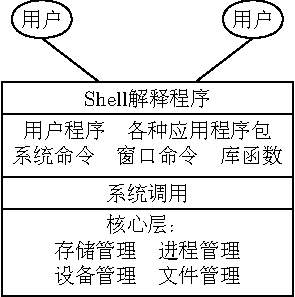
\includegraphics{graph/unix-0.pdf}
  \caption{Unix/Linux结构图(测试图形)}
  \label{fig:UnixTopo}
\end{figure}

\subsection{图片欣赏}
\label{subsec:picView}

下面给出几张美图看看。它们分别是Gnu的logo,内核Linux的logo,还有我最喜
欢的理查德的照片,最后一张是我在网上找到的,自己稍作了处理,嘻嘻……!

\begin{figure}[!htbp]
  \centering
  \subfloat[Gnu Logo]{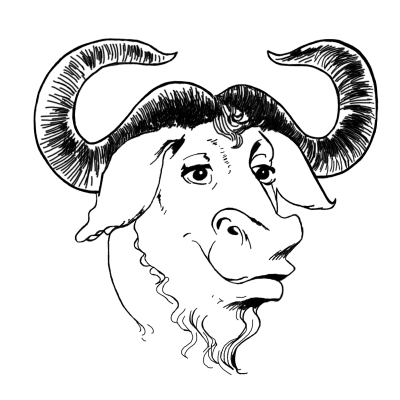
\includegraphics[width=.36\textwidth]{img/gnulogo.png}}
  \subfloat[Linux Logo]{
\includegraphics[width=.34\textwidth]{img/linuxlogo.png}}\hspace{30pt}
  \subfloat[Richard]{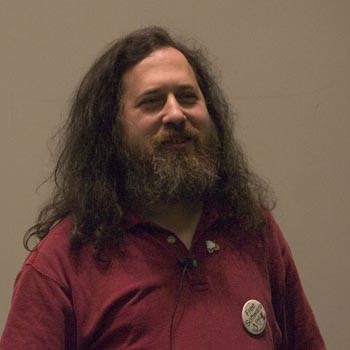
\includegraphics[width=.3328\textwidth]{img/stallman.jpg}}\vspace{10pt}
  \subfloat[网友恶搞]{
\includegraphics[width=.36\textwidth]{img/lw.png}}
  \caption{美图欣赏}
  \label{fig:meituxinshang}
\end{figure}

\section{本书使用的操作系统及环境}
\label{sec:thisOS}

本书的所有操作是在作者笔记本上的虚拟机上演示,虚拟机操作系统
为CentOS7u6 64位,使用三台虚拟机,每台虚拟机两块网卡,一块是NAT\footnote{或者使用桥接的模式也行}模式的网卡,
主要为了虚拟机可以上网;另一块网卡是Internal模式,用来虚拟机之间通信。

\begin{table}[htbp]
  \centering
    \caption{本书所使用的机器一览}
    \label{tab:allMachines}
    \begin{tabular}{llr}
      \toprule
      主机名     & IP地址 & 说明 \\
      \midrule
      node01.lavenliu.cn  & 192.168.56.101 &  主DNS \\
      node02.lavenliu.cn  & 192.168.56.102 &  辅DNS \\
      node03.lavenliu.cn  & 192.168.56.103 &  客户端 \\
      \bottomrule
    \end{tabular}
\end{table}

\subsection{系统环境设置}
\label{sec:osSetup}

\begin{itemize}
  \item 主机名设置,使用 FQDN 形式的域名;
  \item NTP对时,确保每个节点的时间是一致的;
  \item SSH免密码登陆设置;
\end{itemize}

具体操作如下:

\begin{verbatim}
[root@node01 ~]# hostnamectl set-hostname node01.lavenliu.cn
[root@node02 ~]# hostnamectl set-hostname node02.lavenliu.cn
[root@node03 ~]# hostnamectl set-hostname node03.lavenliu.cn
# 以下是通用设置
\end{verbatim}

% 第二部分
\chapter{常用命令使用}
\label{sec:BasicCommand}

\section{命令行下的快捷键}
\label{shortcut}

经常在命令行下工作的小伙伴们,可能用的最多的就是两个上下方向键,主要用来调出
历史命令;使用左右箭头使光标向后或向前移动以修改上次使用过的命令。其实
这样做效率并不是很高,有了快捷键可以让我们的效率提高数倍,而且看起来还
更专业、更加Awesome、更加Geek。掌握了这些快捷键,我们可以做到手不离主键
盘区域,完全可以忽略掉键盘上的四个可爱的箭头。当我们熟练之后,会越发喜
欢这种方式。

\subsection{常用快捷键介绍}

下面介绍一些作者在命令行下经常使用的快捷键,这些快捷键在Emacs下面是有同
样的效果的,不信?你可以试试看。其实,Emacs是Gnu/Linux系统下的命令行编
辑器,通过/etc/profile或/etc/bashrc等文件都可以找到相关的设置。

\begin{enumerate}[itemsep=0pt,parsep=0pt]
	\item Ctrl+A\index{Ctrl+A}快捷键
  \begin{quote}
    这里的A可以理解为Head。当我们按下此组合键时,光标就从当前位置移到了
    命令行的起始位置。别只顾着看,动手试试!
  \end{quote}

\item Ctrl+B\index{Ctrl+B}快捷键
  \begin{quote}
    这里的B可以理解为Backward,向后的意思。有时在命令行上,我们把某个命
    令的参数或路径写错了,一般的做法是,使用左箭头,使光标移动到指定的
    位置,然后修改。其实我们完全可以使用Ctrl+B的方式以达到同样的效果。
    别只顾着看,动手试试!
  \end{quote}

\item Ctrl+C\index{Ctrl+C}快捷键
  \begin{quote}
    这个组合键是用来终止当前正在运行的前台进程。在UNIX环境高级编程一书
    上看到了一个用来终止当前运行进程的组合键,是Ctrl+\textbackslash
    \cite{unixenvironment}。别只顾着看,动手试试!
  \end{quote}

\item Ctrl+D\index{Ctrl+D}快捷键
  \begin{quote}
    这个组合键的用途也很广,我主要用此组合键来退出某个程序,如Python、
    MySQL等等。在命令行下意思就不同啦,此时的D可以理解为Delete。按下此
    组合键,会删除当前光标处的字符。别只顾着看,动手试试!
  \end{quote}

\item Ctrl+E\index{Ctrl+E}快捷键
  \begin{quote}
    这里的E可以理解为End。当在命令行按下此组合键时,我们的可爱的光标就
    乖乖地跑到了当前命令行的最后。\marginpar{这是边注一个}
  \end{quote}

\item Ctrl+F\index{Ctrl+F}快捷键
  \begin{quote}
    这里的F可以理解为Forward,向前的意思,等同于按下右箭头。别只顾着看,
    动手试试!
  \end{quote}

\item Ctrl+H\index{Ctrl+H}快捷键
  \begin{quote}
    此组合键相当于键盘上的Backspace键。按下此组合键,它会从当前光标处开
    始向后删除字符。别只顾着看,动手试试!
  \end{quote}

\item Ctrl+J\index{Ctrl+J}快捷键
  \begin{quote}
    此组合键相当于键盘的回车键。按下此组合键,相当于按了一次回车键。在
    Windows的命令行下,Ctrl+M好像是等同于回车键。别只顾看着,动手试试!
  \end{quote}

\item Ctrl+K\index{Ctrl+K}快捷键
  \begin{quote}
    这里的K可以理解为Kill。按下此组合键,会删除从当前光标到本命令行的结
    束的位置的所有字符。别只顾着看,动手试试!
  \end{quote}

\item Ctrl+L\index{Ctrl+L}快捷键
  \begin{quote}
    这里的L可以理解为Clear。按下此组合键相当于执行了clear这条命令,清除
    当前屏幕上的内容。别只顾着看,动手试试!
  \end{quote}

\item Ctrl+N\index{Ctrl+N}快捷键
  \begin{quote}
    这里的N可以理解为Next。这个组合键的作用是用来调出下一条历史命令,与
    之对应的快捷键Ctrl+P是调出上一条历史命令。代替了向下的箭头。别只顾
    着看,动手试试!
  \end{quote}

\item Ctrl+P\index{Ctrl+P}快捷键
  \begin{quote}
    这里的N可以理解为Previous。这个组合键的作用是用来调出上一条历史命令,
    与之对应的快捷键Ctrl+N是调出下一条历史命令。代替了向上的箭头。别只
    顾着看,动手试试!
  \end{quote}

\item Ctrl+R\index{Ctrl+R}快捷键
  \begin{quote}
    这个组合键是用来搜索之前的历史命令。这里的R可以理解为Reverse,反向
    的意思。在Emacs里为向后搜索,与之对应的是Ctrl+S快捷键是向前搜索。不
    过Ctrl+S在命令行里却不是这个作用,而是用来锁屏的。别只顾着看,动手
    试试!
  \end{quote}

\item Ctrl+S\index{Ctrl+S}快捷键
  \begin{quote}
    这个组合键在Emacs里为向后搜索,与之对应的是Ctrl+S快捷键是向前搜索。不
    过Ctrl+S在命令行里却不是这个作用,而是用来锁屏的。别只顾着看,动手
    试试!锁了之后怎么解锁呢?可以是试试Ctrl+Q组合键。
  \end{quote}

\item Ctrl+T\index{Ctrl+T}快捷键
  \begin{quote}
    此组合键是交换两个相邻字符的位置。交换的是当前光标处字符及其当前光
    标前面的字符。比如我们不小心把clear命令写成了clera,此时我们也不用
    把ra两个字符删掉,然后再写上正确的。此时使我们的光标位于字符a上,让
    后按下此组合键,是不是神奇的事情发生了?当然,如果光标在行尾,按下
    此组合键,它会交换光标前的两个连续的字符。在Emacs下面,使用Ctrl+X与
    Ctrl+T两个组合键\footnote{先按下Ctrl+X,然后松开X,继续
      按着Ctrl键,然后再按下T键,即可完成两个组合键的操作。别嫌麻烦,习
      惯就好了。},可以交换当前光标行与上一行的位置。别只顾着看,动手试
    试!
  \end{quote}

\item Ctrl+W\index{Ctrl+W}快捷键
  \begin{quote}
    此组合键在Emacs中的作用是剪切选中区域的文本。在命令行上使用该组合键
    则是往后删除一个字符组合。也就是说,删除光标左边的一个字母组合或单
    词。比如,我们在此命令行上使用了命令如下,“service network
    restart”,让我们的光标位于字符串的restart的后面,按下该组合键,看看
    有何效果?是不是变成“service network”了?确实是这样,如果我们使用
    Backspace键的话,则需要使用7次的按键才能达到一个Ctrl+W的组合键的效
    果。嗯,别只顾着看,动手试试?
  \end{quote}

\item Alt+.\index{Alt+.}快捷键
  \begin{quote}
    此组合键是调出上一条命令的最后一个参数。如上一条命是“service
    network restart”,则“restart”就是最后一个参数。如果我们接下来要敲的
    命令需要用到上一条命令的最后一个参数,则可使用此快捷键,而不需要手
    工输入“restart”了,而且不会出错,节省敲击键盘的次数。如果我们接下来
    想重启httpd服务,则只需要输入“service httpd ”,然后按下“Alt+.”即可
    补全上一条命令的“restart”。在有些终端上,按“Alt+.”组合键可能会没有
    效果,这时可以使用“ESC+.”组合键代替。在Emacs中,ESC键与Alt键是等价
    的。可以动手试试该组合键的效果。
  \end{quote}

\end{enumerate}


\section{使用man page获得帮助}
\label{sec:getHelp}

当我们遇到不会用的系统命令时,该怎么办呢?或许你第一个想到的
是百度或谷歌,这样想很正常,可以节省很多时间。如果每次遇到不会的命令,
都去找网络,个人觉得这不是一件好的事情,不利于我们自身的提高。
在开源界遇到了问题,有一句口号是:“有问题,找男人\footnote{并不是真男人,而是man page}”。

如果不依靠互联网,该怎么解决呢?那就是依赖系统自带的man page\index{man
  page}了。通过它我们可以获取绝大部分的系统帮助信息。



\section{echo与终端颜色}
\label{sec:echoCmd}

echo\index{echo}会将输入的字符串送往标准输出。输出的字符串间以空白字符隔开, 并在最
后加上换行号。

参数:

\begin{enumerate}[itemsep=0pt,parsep=0pt]
\item \-n 不要在最后自动换行 
\item \-e 若字符串中出现以下字符,则特别加以处理,而不会将它当成一般文字输出: 
\begin{verbatim}
\a 发出警告声; 
\b ***前一个字符; 
\c 最后不加上换行符号; 
\f 换行但光标仍旧停留在原来的位置; 
\n 换行且光标移至行首; 
\r 光标移至行首,但不换行; 
\t 插入tab; 
\v 与\f相同; 
\\ 插入\字符; 
\nnn 插入nnn(八进制)所代表的ASCII字符; 
–help 显示帮助 
–version 显示版本信息
\end{verbatim}
\end{enumerate}

\subsection{终端颜色}

echo字体颜色和背景颜色 

-e enable interpretation of the backslash-escaped characters listed below 

字背景颜色范围:40-47

\begin{table}[!htbp]
  \centering
  \begin{tabular}{llll}
    \toprule
    R & G & B & Color \\
    \midrule
    0 & 0 & 0 & Black \\
    0 & 0 & 1 & Blue \\
    0 & 1 & 0 & Green \\
    0 & 1 & 1 & Cyan \\
    1 & 0 & 0 & Red \\
    1 & 0 & 1 & Magenta \\
    1 & 1 & 0 & Yellow \\
    1 & 1 & 1 & White \\
    \bottomrule
  \end{tabular}
  \caption{颜色表\cite{computersystem}}
  \label{tab:colorTable}
\end{table}

\begin{verbatim}
40:黑 
41:深红 
42:绿 
43:*** 
44:蓝色 
45:紫色 
46:深绿 
47:白色
\end{verbatim}

字颜色:30-37

ANSI控制码的说明:

\begin{verbatim}
\e[0m 关闭所有属性 
\e[1m 设置高亮度 
\e[4m 下划线 
\e[5m 闪烁 
\e[7m 反显 
\e[8m 消隐 
\e[30m — \e[37m 设置前景色 
\e[40m — \e[47m 设置背景色 
\e[nA 光标上移n行 
\e[nB 光标下移n行 
\e[nC 光标右移n行 
\e[nD 光标左移n行 
\e[y;xH设置光标位置 
\e[2J 清屏 
\e[K 清除从光标到行尾的内容 
\e[s 保存光标位置 
\e[u 恢复光标位置 
\e[?25l 隐藏光标 
\e[?25h 显示光标
\end{verbatim}

下面看一个例子:
\begin{verbatim}
for i in `seq 0 7` ; do echo -e "\033[30;4${i}m      \033[0m"; \ 
done
\end{verbatim}

输出结果为:
\begin{figure}[hbtp]
  \centering
  
\includegraphics[width=.15\textwidth]{img/color.png}
  \caption{终端颜色效果}
  \label{fig:TermColor}
\end{figure}


\section{date命令的使用}
\label{sec:dateCmd}

\index{date}

\small{
\begin{verbatim}
# 设日期
date -s 20091112                     

# 设时间
date -s 18:30:50                     

# 7天前日期
date -d "7 days ago" +%Y%m%d         

# 5分钟前时间
date -d "5 minute ago" +%H:%M        

# 一个月前
date -d "1 month ago" +%Y%m%d        

# 日期格式转换
date +%Y-%m-%d -d '20110902'         

# 日期和时间
date +%Y-%m-%d_%X                    

# 纳秒
date +%N                             

# 换算成秒计算(1970年至今的秒数)
date -d "2012-08-13 14:00:23" +%s    

# 将时间戳换算成日期
date -d "@1363867952" +%Y-%m-%d-%T   

# 将时间戳换算成日期
date -d "1970-01-01 UTC 1363867952 seconds" +%Y-%m-%d-%T  

# 格式化系统启动时间(多少秒前)
date -d "`awk -F. '{print $1}' /proc/uptime` second ago" +"%Y-%m-%d %H:%M:%S"    
\end{verbatim}
}
\normalsize

\section{yum命令的使用}
\label{sec:yumCmd}
\index{yum}
安装好系统时,在/etc/yum.repos.d目录下回有一个rhel-debuginfo.repo的文件,
我们这里以redhat系统为例进行讲解。不管这个配置文件的名字如何,但文件的
扩展名须为.repo,如redhat.repo也是可以的。我们需要做一些准备工作。

准备系统镜像文件并挂载到本地:

\small{
\begin{verbatim}
[root@iLiuc ~]# ls 
rhel-server-5.5-i386-dvd.iso

[root@iLiuc ~]# mount -o loop rhel-server-5.5-i386-dvd.iso /media
\end{verbatim}
}
\normalsize

复制镜像里的文件到本地目录:

\begin{verbatim}
[root@iLiuc ~]# mkdir /iso
[root@iLiuc ~]# cp -r /media/* /iso
\end{verbatim}

修改这个配置文件:

\begin{verbatim}
[root@iLiuc ~]# cat /etc/yum.repos.d/rhel-debuginfo.repo
[rhel-debuginfo]
name=Red Hat Enterprise Linux $releasever - $basearch - Debug
baseurl=file:///iso/Server
enabled=1
gpgcheck=0
\end{verbatim}

几点说明:

\begin{quote}
    1. [rhel-debuginfo] 中括号里的内容可以随意写 \\
    2. name 这一行可有可无 \\
    3. baseurl 这行要指定我们的资源在哪里 \\
    4. file:// 说明我们使用什么协议,也可以是ftp://等 \\
    5. /iso/Server 指明我们的源在 /iso/Server 目录下
\end{quote}

配置好之后,如何使用呢?直接看操作吧:

\begin{enumerate}[itemsep=0pt,parsep=0pt]
\item 列出我们有哪些yum仓库
  \small{
\begin{verbatim}
[root@iLiuc ~]# yum repolist
\end{verbatim}
  }
  \normalsize

\item 列出仓库里的包
\begin{verbatim}
[root@iLiuc ~]# yum list
Deployment_Guide-en-US.noarch    5.2-11               installed     
GConf2.i386                      2.14.0-9.el5         installed     
ImageMagick.i386                 6.2.8.0-4.el5_1.1    installed     
MAKEDEV.i386                     3.23-1.2             installed     
NetworkManager.i386              1:0.7.0-10.el5       installed     
NetworkManager-glib.i386         1:0.7.0-10.el5       installed     
NetworkManager-gnome.i386        1:0.7.0-10.el5       installed     
ORBit2.i386                      2.14.3-5.el5         installed    
....
yum-utils.noarch                 1.1.16-13.el5        rhel-debuginfo
yum-verify.noarch                1.16-13.el5          rhel-debuginfo
yum-versionlock.noarch           1.1.16-13.el5        rhel-debuginfo
zisofs-tools.i386                1.0.6-3.2.2          rhel-debuginfo
zsh.i386                         4.2.6-3.el5          rhel-debuginfo
zsh-html.i386                    4.2.6-3.el5          rhel-debuginfo
\end{verbatim}
\end{enumerate}

一些说明:
\begin{quote}
    1. 第一列是我们的软件包名 \\
    2. 第二列是对应软件包的版本号 \\
    3. 第三列 \\
    + installed表明该软件包已安装 \\
    + rhel-debuginfo表明包未安装 
\end{quote}

几个常用的yum命令:
\begin{table}[!htbp]
  \centering
    \caption{yum常用命令选项}
    \begin{tabular}{ll}
      \toprule
      命令           & 说明 \\
      \midrule
      repolist       & 列出我们有哪些yum仓库 \\
      list           & 列出仓库里有哪些软件包 \\
      install        & 安装软件包的命令 \\
      groupinstall   & 安装软件包组 \\
      erase          & 移除一个或多个软件包 \\
      whatprovides   & 查询一个命令属于哪个安装包 \\
      \bottomrule
    \end{tabular}
\end{table}

\subsection{一些实例}
\label{sec:yumExamples}

% \section{zypper命令的使用}
\label{sec:zypperCmd}

\subsection{zypper本地源的配置}
\label{subsec:zypperLocalrepo}

SUSE的zypper本地源配置起来跟yum的配置很相似,它们的配置文件有很多相似之
处。不过,个人觉得zypper这个工具稍微强大些。在SUSE下,可以通过一条
zypper的命令,即可完成zypper源的配置。

为什么会有本节内容呢?主要是2014年9月26日,Bash爆出了一个漏洞,传闻比
“心脏出血”漏洞还要猛,不知道是不是真的。以下是网上给出的验证方法,测试
环境在我的RHEL6 64bit的虚拟机上,

\small{
\begin{verbatim}
[root@master ~]# env x='() { :;}; echo vulnerable' bash -c "echo this is a test"
vulnerable
this is a test
\end{verbatim}
}
\normalsize

同样,在我的SUSE 11sp2 64bit上运行也是同样的输出,输出内容略。以下几个
包是SUSE的OEM厂商给出的Bash最新的升级包。

\begin{verbatim}
funny:~ # unzip CVE-2014-6271.zip 
Archive:  CVE-2014-6271.zip
   creating: CVE-2014-6271/
  inflating: CVE-2014-6271/bash 9740.htm  
  inflating: CVE-2014-6271/bash-3.2-147.20.1.x86_64.rpm  
  inflating: CVE-2014-6271/bash-doc-3.2-147.20.1.x86_64.rpm  
  inflating: CVE-2014-6271/libreadline5-32bit-5.2-147.20.1.x86_64.rpm  
  inflating: CVE-2014-6271/libreadline5-5.2-147.20.1.x86_64.rpm  
  inflating: CVE-2014-6271/license_agreement.txt  
  inflating: CVE-2014-6271/readline-doc-5.2-147.20.1.x86_64.rpm
\end{verbatim}

接下来的操作是把这些包放到一个目录里,然后把该目录做成系统的一个更新源。
比如,把解压后的目录放到/opt目录下,然后使用zypper ar添加该zypper源。

\small{
\begin{verbatim}
funny:~ # mv CVE-2014-6271 /opt/update
funny:~ # zypper ar file:///opt/update update
Adding repository 'update' [done]
Repository 'update' successfully added
Enabled: Yes
Autorefresh: No
GPG check: Yes
URI: file:/opt/update
\end{verbatim}
}
\normalsize

接下来,使用zypper lr验证下,

\small{
\begin{verbatim}
funny:~ # zypper lr
# | Alias  | Name   | Enabled | Refresh
--+--------+--------+---------+--------
1 | local  | local  | Yes     | Yes    
2 | update | update | Yes     | No
\end{verbatim}
}
\normalsize

说明我们已成功添加update的源。另外,执行”zypper ar URI alias“后,会在
/etc/zypp/repo.d/目录下生成alias.repo配置文件。接下来,我们试试zypper
update命令,看是不是可以真的可以升级?

\small{
\begin{verbatim}
funny:~ # zypper update
Building repository 'update' cache [done]
Loading repository data...
Reading installed packages...

The following packages are going to be upgraded:
  bash bash-doc libreadline5 readline-doc 

The following packages are not supported by their vendor:
  bash bash-doc libreadline5 readline-doc 

4 packages to upgrade.
Overall download size: 923.0 KiB. ...
Continue? [y/n/?] (y): y
Retrieving package libreadline5-5.2-147.20.1.x86_64 (1/4), ...
Retrieving package bash-3.2-147.20.1.x86_64 (2/4), ...
Retrieving package readline-doc-5.2-147.20.1.x86_64 (3/4), ...
Retrieving package bash-doc-3.2-147.20.1.x86_64 (4/4), ...
Retrieving package libreadline5-5.2-147.20.1.x86_64 (1/4), ...
Installing: libreadline5-5.2-147.20.1 [done]
Retrieving package bash-3.2-147.20.1.x86_64 (2/4), ...
Installing: bash-3.2-147.20.1 [done]
Retrieving package readline-doc-5.2-147.20.1.x86_64 (3/4), ...
Installing: readline-doc-5.2-147.20.1 [done]
Retrieving package bash-doc-3.2-147.20.1.x86_64 (4/4), ...
Installing: bash-doc-3.2-147.20.1 [done]
\end{verbatim}
}
\normalsize

以上说明可以进行升级的。接下来,我们使用zypper ps命令,可以查看有哪些终
端还在使用之前没有升级过的bash,

\small{
\begin{verbatim}
funny:/etc/zypp/repos.d # zypper ps
The following running processes use deleted files:

PID   | PPID  | UID | Login | Command | Files                    
------+-------+-----+-------+---------+--------------------------
2663  | 2542  | 0   | root  | bash    | /lib64/libreadline.so.5.2
      |       |     |       |         | /bin/bash (deleted)      
22426 | 22423 | 0   | root  | bash    | /lib64/libreadline.so.5.2
      |       |     |       |         | /bin/bash (deleted)      

You may wish to restart these processes.
\end{verbatim}
}
\normalsize

说明还有bash升级前的两个进程还在运行,我们可以退出这两个终端,再次登入
系统,再次使用zypper ps命令来查看,就会看到”No processes using deleted
files found.“的提示。

\subsection{zypper命令选项介绍}
\label{subsec:zypperCmdopt}

zypper\index{zypper}是SuSE\index{SUSE}系列下面的包管理工具,如同
\ref{sec:yumCmd}节的yum工具。

zypper的几个重要选项:

\begin{table}[!htbp]
  \centering
    \caption{zypper安装源操作选项}
    \begin{tabular}{ll}
      \toprule
      选项           & 说明 \\
      \midrule
      repos, lr      & 列出库 \\
      addrepo, ar    & 添加库 \\
      renamerepo, nr & 重命名指定的安装源 \\
      modifyrepo, mr & 修改指定的安装源 \\
      refresh, ref   & 刷新所有安装源 \\
      clean          & 清除本地缓存 \\
      \bottomrule
    \end{tabular}
\end{table}

举例说明,

列出当前有哪些库,

\begin{verbatim}
# zypper lr
# | Alias       | Name        | Enabled | Refresh
--+-------------+-------------+---------+--------
1 | 6271        | 6271        | Yes     | No     
2 | 7169        | 7169        | Yes     | No     
3 | SUSE11SP2   | SUSE11SP2   | Yes     | No     
4 | cve20150235 | cve20150235 | Yes     | No
\end{verbatim}

添加本地库,

\begin{verbatim}
# zypper ar file:///opt/patch/ mypatch
Adding repository 'mypatch' [done]
Repository 'mypatch' successfully added
Enabled: Yes
Autorefresh: No
GPG check: Yes
URI: file:/opt/patch/

# zypper lr
# | Alias       | Name        | Enabled | Refresh
--+-------------+-------------+---------+--------
1 | 6271        | 6271        | Yes     | No     
2 | 7169        | 7169        | Yes     | No     
3 | SUSE11SP2   | SUSE11SP2   | Yes     | No     
4 | cve20150235 | cve20150235 | Yes     | No
5 | mypatch     | mypatch     | Yes     | No
\end{verbatim}

zypper的查询选项:

\begin{table}[!htbp]
  \centering
    \caption{zypper工具查选选项}
    \begin{tabular}{ll}
      \toprule
      选项              & 说明 \\
      \midrule
      search, se        & 安装软件包 \\
      info, if          & 查看软件包信息 \\
      packages, pa      & 列出所有可用的软件包 \\
      patterns, pt      & 列出所有可用的模式 \\
      products, pd      & 列出所有可用的产品 \\
      what-provides, wp & 列出能够提供指定功能的软件包 \\
      \bottomrule
    \end{tabular}
\end{table}

举例说明,

\begin{verbatim}
# zypper se snmp
Building repository 'mypatch' cache [done]
Loading repository data...
Reading installed packages...

S | Name                | Summary                         | Type      
--+---------------------+---------------------------------+-----------
i | libsnmp15           | Shared Libraries from net-snmp  | package   
  | libsnmp15-32bit     | Shared Libraries from net-snmp  | package   
i | net-snmp            | SNMP Daemon                     | package   
  | net-snmp            | SNMP Daemon                     | srcpackage
  | perl-Net-SNMP       | Net::SNMP Perl Module           | package   
  | perl-Net-SNMP       | Net::SNMP Perl Module           | srcpackage
i | perl-SNMP           | Perl-SNMP                       | package   
  | php5-snmp           | PHP5 Extension Module           | package   
  | php53-snmp          | PHP5 Extension Module           | package   
  | rsyslog-module-snmp | SNMP support module for rsyslog | package   
i | snmp-mibs           | MIB files from net-snmp         | package
#
# zypper if net-snmp
Loading repository data...
Reading installed packages...


Information for package net-snmp:

Repository: SUSE-Linux-Enterprise-Server-11-SP2 11.2.2-1.234
Name: net-snmp
Version: 5.4.2.1-8.12.6.1
Arch: x86_64
Vendor: SUSE LINUX Products GmbH, Nuernberg, Germany
Support Level: Level 3
Installed: Yes
Status: up-to-date
Installed Size: 1.0 MiB
Summary: SNMP Daemon
Description: 
This package was originally based on the CMU 2.1.2.1 snmp verbatim.It has been greatly modified, restructured, enhanced, and fixed.It hardly looks the same as anything that CMU has ever released.It was renamed from cmu-snmp to ucd-snmp in 1995 and later renamedfrom ucd-snmp to net-snmp in November 2000.
#
\end{verbatim}

zypper软件管理:

\begin{table}[!htbp]
  \centering
    \caption{zypper软件管理选项}
    \begin{tabular}{ll}
      \toprule
      选项               & 说明 \\
      \midrule
      install, in        & 安装软件包 \\
      remove, rm         & 删除软件包 \\
      verify, ve         & 检验软件包依赖关系的完整性 \\
      update, up         & 更新已安装的软件包到新的版本 \\
      dist-upgrade, dup  & 整个系统的升级 \\
      source-install, si & 安装源代码软件包和它们的编译依赖 \\
      \bottomrule
    \end{tabular}
\end{table}

举例说明,

\begin{verbatim}
# zypper rm net-snmp
Loading repository data...
Reading installed packages...
Resolving package dependencies...

The following packages are going to be REMOVED:
  net-snmp perl-SNMP 

2 packages to remove.
After the operation, 1.6 MiB will be freed.
Continue? [y/n/?] (y): y
Removing perl-SNMP-5.4.2.1-8.12.6.1 [done]
Removing net-snmp-5.4.2.1-8.12.6.1 [done]
#
# zypper in -y net-snmp
Loading repository data...
Reading installed packages...
Resolving package dependencies...

The following NEW packages are going to be installed:
  net-snmp perl-SNMP 

2 new packages to install.
Overall download size: 543.0 KiB. After the operation, additional 1.6 MiB will be used.
Continue? [y/n/?] (y): y
Retrieving package perl-SNMP-5.4.2.1-8.12.6.1.x86_64 (1/2), 176.0 KiB (609.0 KiB unpacked)
Retrieving package net-snmp-5.4.2.1-8.12.6.1.x86_64 (2/2), 367.0 KiB (1.0 MiB unpacked)
Installing: perl-SNMP-5.4.2.1-8.12.6.1 [done]
Installing: net-snmp-5.4.2.1-8.12.6.1 [done]
Additional rpm output:
Updating etc/sysconfig/net-snmp...
\end{verbatim}



\section{parted命令的使用}
\label{sec:PartedCmd}

Gnu/Linux系统的分区工具通常可以使用fdisk与parted。我们用的比较多的工具
就是fdisk了,这里不介绍它的使用了。这里简单的介绍如何使用parted工具,对
于分区表通常有MBR分区表和GPT分区表对于磁盘大小小于2T的磁盘,我们可以使
用fdisk和parted命令工具进行分区对于MBR分区表的特点(通常使用fdisk命令进
行分区)所支持的最大磁盘大小:2T最多支持4个主分区或者是3个主分区加上一
个扩展分区对于GPT分区表的特点(使用parted命令进行分区)支持最大
卷:18EB(1EB=1024TB)最多支持128个分区。

对于parted命令工具分区的介绍

最后,fdisk与parted有些差异。fdisk分区完毕后,需要使用“w”命令才能保存
之前所做的一些操作;而parted则是实时的,每一步操作不需要保存,即时生
效。


\section{mount命令的使用}
\label{sec:mountCmd}

如何挂载iso镜像文件呢?我们可以使用一下mount\index{mount}命令:

\small{
\begin{verbatim}
[root@iLiuc ~]# mount -o loop rhel-server-5.5-i386-dvd.iso /mnt
# 意思是把当前目录下的rhel-server-5.5-i386-dvd.iso挂载到/mnt目录下
\end{verbatim}
}
\normalsize


\section{grep命令的使用}
\label{sec:grepCmd}

grep\index{grep}(global regular expression pattern的缩写)。其实可以把它
理解为过滤关键字用的一个程序。具体怎么用,还是看一个实例吧,然后结束本
节内容。

\subsection{常用选项}

\begin{table}[!htbp]
  \centering
  \caption{grep常用选项}
  \begin{tabular}{l|l}
    \hline
    -A NUM  & 打印出紧随匹配的行之后的下文NUM行 \\
    \hline
    -B NUM  & 打印出匹配的行之前的上文NUM行 \\
    \hline
    -C NUM  & 打印出匹配的行的上下文前后各NUM行 \\
    \hline
    -b      & 在输出的每行前面同时打印出当前行在输入文件中的字节偏移量 \\
    \hline
    -c      & 显示匹配的行数 \\
    \hline
    -f file & 从文件file中获取模式,每行一个 \\
    \hline
    -H      & 为每个匹配的文件打印文件名 \\
    \hline
    -I      & 不搜索二进制文件 \\
    \hline
    -i      & 忽略大小写 \\
    \hline
    -l      & 只显示有匹配的文件的文件名 \\
    \hline
    -L      & 只显示未匹配的文件的文件名 \\
    \hline
    -n      & 输出行号 \\
    \hline
    -o      & 只显示匹配字段 \\
    \hline
    -q      & quiet静默模式 \\
    \hline
    -v      & 只显示不匹配的行 \\
    \hline
  \end{tabular}
\end{table}

\subsection{一些实例}

去掉文件里的注释行和空白行
\begin{verbatim}
# cat filename | grep -v ^$ | grep -v ^# | sudo tee squid.conf
\end{verbatim}

这里我们使用grep命令及cut命令一起把eth0上的IP给取出来,看操作:

\begin{verbatim}
  [root@iLiuc ~]# ifconfig eth0
  eth0 Link encap:Ethernet  HWaddr 5A:B6:4E:85:55:44  
  inet addr:192.168.18.18  Bcast:192.168.18.255  Mask:255.255.255.0
  inet6 addr: fe80::58b6:4eff:fe85:5544/64 Scope:Link
  UP BROADCAST RUNNING MULuTICAST  MTU:1500  Metric:1
  RX packets:11655331 errors:0 dropped:0 overruns:0 frame:0
  TX packets:1074797 errors:0 dropped:0 overruns:0 carrier:0
  collisions:0 txqueuelen:1000 
  RX bytes:4001012028 (3.7 GiB)  TX bytes:628740073 (599.6 MiB)
  Interrupt:185

  # 使用grep命令,匹配关键字,缩小范围
  [root@iLiuc ~]# ifconfig eth0 |grep "inet addr"
  inet addr:192.168.18.18  Bcast:192.168.18.255  Mask:255.255.255.0

  # 使用cut命令,把范围再次缩小些
  [root@iLiuc ~]# ifconfig eth0 |grep "inet addr" | cut -d: -f2
  192.168.18.18  Bcast

  # 是不是快出来了,再使用cut一次,IP地址就出来了
  [root@iLiuc ~]# 自己写出来吧,我已经写得很多了!
\end{verbatim}


\section{crontab命令的使用}
\label{sec:crontabCmd}

假想这样一个场景:每天的凌晨两点,领导都会要求你你重启服务器(当然,这
有点变态)。这时,你该怎么办?你是不是每天凌晨两点都要从温暖的被窝里爬
出来,然后远程连接服务器,然后重启服务器,然后重新钻进被窝,然后失眠
了...。每天都如此,我想你一定会奔溃的。

crontab\index{crontab}命令可以解救你!crontab几个字段的说明:

\small{
\begin{verbatim}
  field          allowed values
  -----          --------------
  minute         0-59
  hour           0-23
  day of month   1-31
  month          1-12 (or names, see below)
  day of week    0-7 (0 or 7 is Sun, or use names)
\end{verbatim}
}
\normalsize

\small{
\begin{verbatim}
  # 查看当前用户的crontab
  [root@iLiuc ~]# crontab -l
  */2 * * * * /usr/lib/clear-server/cleargard/cleargard.sh
  上面语句的意思是,每2分钟去执行/usr/lib/clear-server/cleargard目录下的
  cleargard.sh脚本,只要系统一直运行,它就会循环往复的执行。

  # 编辑crontab
  [root@iLiuc ~]# crontab -e
\end{verbatim}
}
\normalsize


\section{find命令的使用}

find\index{find}命令很强大,强大到可以写很多东西。这里就介绍如何简单的
使用。直接看例子吧:

\small{
\begin{verbatim}
# linux文件无创建时间
# Access 使用时间  
# Modify 内容修改时间  
# Change 状态改变时间(权限、属主)
# 时间默认以24小时为单位,当前时间到向前24小时为0天,向前48-72小时为2天
# -and 且 匹配两个条件 参数可以确定时间范围 -mtime +2 -and -mtime -4
# -or 或 匹配任意一个条件

# 按文件名查找
find /etc -name http        

# 查找某一类型文件
find . -type f               

# 按照文件权限查找
find / -perm                 

# 按照文件属主查找
find / -user                 

# 按照文件所属的组来查找文件
find / -group                

# 文件使用时间在N天以内
find / -atime -n             

# 文件使用时间在N天以前
find / -atime +n             

# 文件内容改变时间在N天以内
find / -mtime -n             

# 文件内容改变时间在N天以前
find / -mtime +n             

# 文件状态改变时间在N天前
find / -ctime +n             

# 文件状态改变时间在N天内
find / -ctime -n             

# 查找文件长度大于1M字节的文件
find / -size +1000000c -print 

# 按名字查找文件传递给-exec后命令
find /etc -name "passwd*" -exec grep "root" {} \; 

# 查找文件名,不取路径
find . -name 't*' -exec basename {} \;  

# 批量改名(查找err替换为ERR {}文件
find . -type f -name "err*" -exec  rename err ERR {} \; 

# 查找任意一个关键字
find 路径 -name *name1* -or -name *name2* 
\end{verbatim}
}
\normalsize




\section{top命令的使用}
\label{sec:topCmd}

top\index{top}命令可动态显示服务器的进程信息,用户可以通过按键来刷新当
前状态。别的不多说,给个例子看看:

\begin{verbatim}
Tasks: 202 total,   2 running, 199 sleeping,   0 stopped,   1 zombie
Cpu(s):  7.9%us,  1.9%sy,  0.0%ni, 89.5%id,  0.7%wa,  0.0%hi,  0.0%si,  0.0%st
Mem:   6003152k total,  1909420k used,  4093732k free,    73688k buffers
Swap:  6180860k total,        0k used,  6180860k free,   893544k cached

  PID USER      PR  NI  VIRT  RES  SHR S %CPU %MEM    TIME+  COMMAND                                                   
 3852 richard   20   0 1329m 127m  31m S   22  2.2   2:11.41 vlc                                                                 
 2891 richard    9 -11  418m 6988 4660 S    6  0.1   0:37.86 pulseaudio 
 2880 richard   20   0 1669m  90m  35m S    5  1.6   1:35.32 gnome-shell
 2452 root      20   0  303m  74m  61m S    4  1.3   1:23.90 Xorg
 3051 richard   20   0  872m 200m  52m S    1  3.4   1:32.25 firefox
   10 root      20   0     0    0    0 S    0  0.0   0:00.57 rcuos/2
   77 root      20   0     0    0    0 R    0  0.0   0:01.30 kworker/3:1
  909 root     -51   0     0    0    0 S    0  0.0   0:10.11 irq/48-iwlwifi
 3025 richard   20   0  581m  19m  11m S    0  0.3   0:01.72 gnome-terminal
 3942 richard   20   0 99.6m  15m 5028 S    0  0.3   0:02.35 python
 4025 richard   20   0 17460 1408  980 R    0  0.0   0:00.04 top
    1 root      20   0 24740 2620 1352 S    0  0.0   0:00.88 init
    2 root      20   0     0    0    0 S    0  0.0   0:00.00 kthreadd
    3 root      20   0     0    0    0 S    0  0.0   0:00.08 ksoftirqd/0
    5 root       0 -20     0    0    0 S    0  0.0   0:00.00 kworker/0:0H                                                                            
    6 root      20   0     0    0    0 S    0  0.0   0:01.68 kworker/u16:0
    7 root      20   0     0    0    0 S    0  0.0   0:01.60 rcu_sched
    8 root      20   0     0    0    0 S    0  0.0   0:01.24 rcuos/0
    9 root      20   0     0    0    0 S    0  0.0   0:00.45 rcuos/1
   11 root      20   0     0    0    0 S    0  0.0   0:00.28 rcuos/3
   12 root      20   0     0    0    0 S    0  0.0   0:00.00 rcuos/4
   13 root      20   0     0    0    0 S    0  0.0   0:00.00 rcuos/5
   14 root      20   0     0    0    0 S    0  0.0   0:00.00 rcuos/6
   15 root      20   0     0    0    0 S    0  0.0   0:00.00 rcuos/7
   16 root      20   0     0    0    0 S    0  0.0   0:00.00 rcu_bh
\end{verbatim}

\section{free命令的使用}
\label{sec:freeCmd}

\subsection{常用选项}
\label{subsec:freeOptions}

free 命令是查看系统内存的使用情况的。下面介绍几个常用的选项,

\begin{table}[htbp]
  \centering
    \caption{free常用选项}
    \label{tab:freeSomeOpts}
    \begin{tabular}{cl}
      \toprule
      选项     & 说明 \\
      \midrule
      -m        & 以 MB 为单位显示当前系统的内存使用情况 \\
      -g        & 以 GB 为单位显示当前系统的内存使用情况 \\
      \bottomrule
    \end{tabular}
\end{table}

\subsection{一些实例}
\label{subsec:freeInstances}



\section{xargs命令的使用}
\label{sec:xargsCmd}
\index{xargs}

\section{tr命令的使用}
\label{sec:trCmd}
\index{tr}

\section{tar命令的使用}
\label{sec:tarCmd}

tar\index{tar}命令是一个打包与解包的一个工具,功能很强大。下面介绍一些常用选项及使
用示例。

通用选项:

\begin{table}[htbp]
  \centering
    \caption{tar通用选项}
    \label{tab:tarGeneralOpt}
    \begin{tabular}{cl}
      \toprule
      选项     & 说明 \\
      \midrule
      j        & 使用bzip2的压缩方式 \\
      t        & 列出压缩包里有哪些文件,并不解压 \\
      z        & 使用gzip的压缩方式 \\
      f        & 指定输出的结果文件。该选项是必选的,不管是压缩还是解压缩 \\
      p        & 保留文件的所有权限 \\
      v        & 压缩或解压缩时,查看其打包过程 \\
      \bottomrule
    \end{tabular}
\end{table}

压缩时用的选项:

\begin{table}[!htbp]
  \centering
    \caption{tar压缩选项}
    \label{tab:tarCompressOpt}
    \begin{tabular}{cl}
      \toprule
      选项     & 说明 \\
      \midrule
      c        & 打包时用的选项,选项c与x不能同时出现 \\
      \bottomrule
    \end{tabular}
\end{table}

解压缩用的选项:

\begin{table}[htbp]
  \centering
    \caption{tar解压缩选项}
    \label{tab:tarUncompressOpt}
    \begin{tabular}{cl}
      \toprule
      选项     & 说明 \\
      \midrule
      x        & 解包时用的选项,选项c与x不能同时出现 \\
      \bottomrule
    \end{tabular}
\end{table}

举例说明:

\small{
\begin{verbatim}
  [root@iLiuc ~]# ls
  360fy        CLEAR-VOD-INSTALLPACKGE.V.2.0.8.tar
  这里有两个文件,第一个为目录,第二个为压缩包

  1. 创建tar包,不压缩
  [root@iLiuc ~]# tar -cvf 360fy.tar 360fy
  360fy/
  360fy/clearVodMS_360fy.tar.gz
  360fy/vod_yuezizhongxin.tar.gz
  360fy/clear_360fy.sql
  上面的例子我们使用-v选项,使我们可以看到过程。其中360fy.tar是我们创建的tar包,是针对
  360fy这个目录的,后面可以是一个或多个文件。

  2. 创建tar包,以gzip方式压缩
  [root@iLiuc ~]# tar -czvf 360fy.tar.gz 360fy

  3. 创建tar包,以bzip2的方式压缩
  [root@iLiuc ~]# tar -cjvf 360fy.tar.bz2 360fy

  4. 查看压缩包的内容,并不解压缩
  [root@iLiuc ~]# tar -tf 360fy.tar
  360fy/
  360fy/clearVodMS_360fy.tar.gz
  360fy/vod_yuezizhongxin.tar.gz
  360fy/clear_360fy.sql

  5. 解压缩
  不管是tar包,还是以gzip或bz2压缩的方式,我们使用一下这条命令都是通用的
  [root@iLiuc ~]# tar -xf 360fy.tar
  [root@iLiuc ~]# tar -xf 360fy.tar.gz
  [root@iLiuc ~]# tar -xf 360fy.tar.bz2
  这里我们没有加-v选项,可以加上-v选项以看到解压过程
\end{verbatim}
}
\normalsize


\section{read命令的使用}
\label{sec:readCmd}
\index{read}

\subsection{常用选项}

\subsection{一些实例}

\section{cut命令的使用}
\label{sec:cutCmd}

cut\index{cut}命令有的时候很有用,比如要获得指定的以某个分隔符分割的列
时,它就可以做到。其实还有比它更强大的工具,如sed及awk等,这里并不介绍
它们,后续章节有介绍。这里就不提及了,跳过它们吧。下面直接看例子吧:

\subsection{常用选项}
\label{subsec:cutOptions}

下面介绍几个常用的cut命令的选项,

\begin{table}[htbp]
  \centering
    \caption{cut常用选项}
    \label{tab:cutSomeOpts}
    \begin{tabular}{cl}
      \toprule
      选项     & 说明 \\
      \midrule
      -c        & 按照字符进行分割 \\
      -d        & 指定分割字段的分隔符,默认是tab \\
      -f        & 指定要显示的列 \\
      \bottomrule
    \end{tabular}
\end{table}

\subsection{一些实例}
\label{subsec:cutInstances}

接下来演示cut命令的一些常用示例,比如我们要查看/etc/passwd文件中用户名,由于用户名是位于/etc/passwd文件中的每一行的第一个以冒号为分割的字段,因此,可以使用cut命令轻松实现取出用户名的需求,

\begin{verbatim}
# cut -d: -f1 /etc/passwd

-d 指定区分列的定界,默认是tab
-f 指定要显示的列
-c 按字符来切割,如
# cut -c1-6 file (取文件第一行的前6个字符)

实验:取IP地址
# ifconfig wlan0 | grep 'inet addr' | cut -d: -f2 | cut -d' ' -f1
# hostname -i[I]

# 显示系统中总内存量
# free |tr -s ' ' |sed '/^Mem/!d' |cut -d" " -f2
\end{verbatim}


\begin{verbatim}
[root@iLiuc ~]# cat test.txt
chuanchuan:goodboy
chuanchuan goodboy

# 以冒号为分割,显示第一列
[root@iLiuc ~]# cut -d: -f1 test.txt
chuanchuan
chuanchuan goodboy

# 以冒号为分割,显示第二列
[root@iLiuc ~]# cut -d: -f2 test.txt
goodboy
chuanchuan goodboy

# 以空格为分割,显示第一列
[root@iLiuc ~]# cut -d" " -f1 test.txt
chuanchuan:goodboy
chuanchuan
\end{verbatim}

我想,知道这么多,应该就可以了。


\section{sort命令的使用}
\label{sec:sortCmd}
\index{sort}

\subsection{常用选项}
\label{subsec:sortOptions}

下面介绍几个常用的cut命令的选项,

\begin{table}[htbp]
  \centering
    \caption{sort常用选项}
    \label{tab:sortSomeOpts}
    \begin{tabular}{cl}
      \toprule
      选项     & 说明 \\
      \midrule
      -c        & 按照字符进行分割 \\
      -d        & 指定分割字段的分隔符,默认是tab \\
      -f        & 指定要显示的列 \\
      \bottomrule
    \end{tabular}
\end{table}

\subsection{一些实例}
\label{subsec:sortInstances}

\section{lsof命令的使用}
\label{sec:lsofCmd}
\index{lsof}

lsof\index{lsof}是“list open files”的缩写,是一个列出当前系统打开文件的
工具。在linux环境下,任何事物都以文件的形式存在,通过文件不仅仅可以访问
常规数据,还可以访问网络连接和硬件。所以如传输控制协议 (TCP) 和用户数据
报协议(UDP) 套接字等,系统在后台都为该应用程序分配了一个文件描述符,无
论这个文件的本质如何,该文件描述符为应用程序与基础操作系统之间的交互提
供了通用接口。因为应用程序打开文件的描述符列表提供了大量关于这个应用程
序本身的信息,因此通过lsof工具能够查看这个列表对系统监测以及排错将是很
有帮助的。

lsof不加任何选项,默认输出所有活动进程打开的文件。

\begin{verbatim}
show all connections with -i

# lsof -i
COMMAND  PID USER   FD   TYPE DEVICE SIZE NODE NAME
dhcpcd  6061 root   4u   IPv4   4510       UDP *:bootpc
sshd    7703 root   3u   IPv6   6499       TCP *:ssh (LISTEN)
sshd    7892 root   3u   IPv6   6757       TCP 10.10.1.5:ssh->192.168.1.5:49901 (ESTABLISHED)

# Get only IPv6 traffic with -i 6
# lsof -i 6

# show only tcp connections (works the same for udp)
# lsof -iTCP

# show networking related to a given port using -i :port
# lsof -i :22

# show connections to a specific host using @host
# lsof -i@172.16.25.18

# show connections based on the host and the port using @host:port
# lsof -i@172.16.25.18:22

# Find listening ports
# find ports that are awaiting connections
# lsof -i -sTCP:LISTEN

# User Information

# We can also get information on various users and what they're doing
# on the system, including their activity on the network, their
# interactions with files, etc.

# show what a given user has open using -u
# lsof -u postfix

# show what all users are doing except a certain user using -u ^user
# lsof -u ^postfix

# Kill everything a given user is doing
# kill -9 `lsof -t -u postfix`
\end{verbatim}

\subsection{恢复删除的文件}

有一次做研发的一位同事,因为系统根目录空间不足,想释放磁盘空间,结果使
用find命令找到了单个文件大于1GB的文件,发现/var/log/messages和
/var/log/warn文件每个都是1.3GB。他的系统根目录空间只有50GB的容量,结果
把/var/log/messages日志文件及/var/log/warn日志文给删除了。删除之后,却
没有达到的目的,磁盘使用空间依然是100\%。

殊不知,当进程打开了某个文件时,只要该进程保持打开该文件,即使将其删除,
它依然存在于磁盘中。这意味着,进程并不知道文件已经被删除,它仍然可以向
打开该文件时提供给它的文件描述符进行读取和写入。除了该进程之外,这个文
件是不可见的,因为已经删除了其相应的目录条目。

拿/var/log/messages文件为例,看看如何在故意删除后如何找回来。我们先看一
下/var/log/messages文件是什么进程打开的。

\begin{verbatim}
[root@iLiuc ~]# lsof /var/log/messages 
COMMAND    PID USER   FD   TYPE DEVICE SIZE/OFF    NODE NAME
syslog-ng 1493 root   10w   REG    8,2 57599903 3080573 /var/log/messages
\end{verbatim}

该命令的输出表明,/var/log/messages文件由syslog-ng进程打开,当前的进程
号为1493,用户身份是root,打开的文件描述符为10且该文件处于只写模式,对
应的TYPE(类型)为REG(常规)文件、磁盘位置、文件大小、索引节点。下面一
一验证:

\begin{verbatim}
[root@iLiuc ~]# stat /var/log/messages 
  File: `/var/log/messages'
  Size: 57603503  	Blocks: 112632     IO Block: 4096   regular file
Device: 802h/2050d	Inode: 3080573     Links: 1
Access: (0640/-rw-r-----)  Uid: (    0/    root)   Gid: (    0/    root)
Access: 2015-03-12 15:33:28.000000000 +0800
Modify: 2015-03-12 16:02:01.000000000 +0800
Change: 2015-03-12 16:02:01.000000000 +0800
 Birth: -
\end{verbatim}

现在,我们可以删除该文件以模拟误删除,

\begin{verbatim}
[root@iLiuc ~]# rm -f /var/log/messages
[root@iLiuc ~]# lsof -n |grep '(deleted)'
syslog-ng 1493  root 10w  REG  8,2 57605375   3080573 /var/log/messages (deleted)
\end{verbatim}

文件已被删除,看怎么恢复吧!从上面的输出信息可以看出之前打开该文件的进
程号及文件描述符,有了这两个信息就足够了。接下来,我们去cat一下/proc目
录中相应的目录中的文件描述符,

\begin{verbatim}
[root@iLiuc ~]# cat /proc/1493/fd/10 |head
Oct  9 03:55:32 linux syslog-ng[5747]: syslog-ng starting up; version='2.0.9'
Oct  9 03:55:32 linux syslog-ng[5747]: syslog-ng starting up; version='2.0.9'
Oct  9 03:55:32 linux syslog-ng[5747]: syslog-ng starting up; version='2.0.9'
Oct  9 03:55:32 linux syslog-ng[5747]: syslog-ng starting up; version='2.0.9'
Oct  9 03:55:32 linux syslog-ng[5747]: syslog-ng starting up; version='2.0.9'
Oct  9 03:55:32 linux syslog-ng[5747]: syslog-ng starting up; version='2.0.9'
Oct  9 03:55:32 linux syslog-ng[5747]: syslog-ng starting up; version='2.0.9'
Oct  9 03:55:32 linux syslog-ng[5747]: syslog-ng starting up; version='2.0.9'
Oct  9 03:55:32 linux syslog-ng[5747]: syslog-ng starting up; version='2.0.9'
Oct  9 03:55:32 linux syslog-ng[5747]: syslog-ng starting up; version='2.0.9'
\end{verbatim}

通过文件描述符查看了相应的数据,那么就可以使用I/O重定向将其复制到文件中,
如cat /proc/1493/fd/10 > /tmp/messages。此时,可以中止该守护进程(这将
  删除 FD,从而删除相应的文件),将这个临时文件复制到所需的位置,然后重
新启动该守护进程。

\begin{verbatim}
[root@iLiuc ~]# cat /proc/1493/fd/10 > /tmp/messages
[root@iLiuc ~]# /etc/init.d/syslog stop
[root@iLiuc ~]# cp /tmp/messages /var/log/messages
[root@iLiuc ~]# /etc/init.d/syslog start
[root@iLiuc ~]# wc -l /var/log/messages 
452113 /var/log/messages

[root@iLiuc ~]# lsof /var/log/messages 
COMMAND    PID USER   FD   TYPE DEVICE SIZE/OFF    NODE NAME
syslog-ng 3819 root    4w   REG    8,2 57608271 3080449 /var/log/messages
\end{verbatim}

我们可以看到,已删除的/var/log/messages文件已回来了!对于许多应用程序,
尤其是日志文件和数据库,这种恢复删除文件的方法非常有用。


\section{netstat命令的使用}
\label{sec:netstatCmd}
\index{netstat}

\section{tcpdump命令的使用}
\label{sec:tcpdumpCmd}

tcpdump\index{tcpdump}是一款基于命令行的工具,可以通过不同的命令行选项
来改变其状态、捕获数据的数量及捕获数据的方法。tcpdump提供的丰富选项可以
使你很容易的改变程序的运行方式。

下面列举一部分比较常用的选项,

\begin{table}[!htbp]
  \centering
  \caption{tcpdump常用选项}
  \label{tab:tcpdumpOptions}
  \begin{tabular}{ll}
    \toprule
    选项     & 说明 \\
    \midrule
    i     & 指定侦听的网络接口 \\
    v     & 指定详细模式输出详细的报文信息 \\
    vv    & 指定非常详细的模式输出及非常详细的报文信息 \\
    vvv   & 指定更加详细的模式输出及更详细的报文信息 \\
    x     & 规定tcpdump以16进制数格式显示数据包 \\
    X     & 规定tcpdump以hex及ASCII格式显示输出 \\
    XX    & 同上,并显示以太网头部信息 \\
    n     & 在捕获过程中不需要向DNS查询IP地址(显示IP地址及端口号) \\
    F     & 从指定的文件中读取表达式 \\
    D     & 显示tcpdump可以侦听的网络接口列表 \\
    c     & 指定捕获多少数据包,然后停止捕获 \\
    w     & 把捕获到的信息写到一个文件中 \\
    s     & 设置捕获数据包的长度为length \\
    \bottomrule
  \end{tabular}
\end{table}

第一种是关于类型的关键字,主要包括host, net, port,例如host
210.27.38.1,指明210.27.38.1是一台主机,net 202.0.0.0指明202.0.0.0是一个
网络地址,port 23指明端口是23。如果没有指定类型,缺省的类型是host。

\small{
\begin{verbatim}
# 想要截获所有210.27.38.1的主机收到的和发出的所有的数据包:
# tcpdump host 210.27.38.1

# 对本机的udp 123端口进行监视,123为ntp的服务端口
# tcpdump udp port 123

# 如果想要获取主机210.27.38.1接收或发出的telnet包,使用如下命令:
# tcpdump tcp port 23 host 210.27.38.1

# 想要获取主机210.27.38.1和主机210.27.38.2或210.27.38.3的通信,使用命令:
# 在命令行中使用括号时,一定要转义
# tcpdump host 210.27.38.1 and \(210.27.38.2 or 210.27.38.3\)

# 如果想要获取主机210.27.38.1除了和主机210.27.38.2之外所有主机通信的ip包,则:
# tcpdump ip host 210.27.38.1 and ! 210.27.38.2

# tcpdump icmp
# tcpdump port 3306
# tcpdump src port 1025
# tcpdump dst port 389
# tcpdump src port 1025 and tcp
# tcpdump udp and src port 53
\end{verbatim}
}
\normalsize


\section{traceroute命令的使用}
\label{sec:tracerouteCmd}

\section{wget命令的使用}
\label{sec:wgetCmd}

通常用来在命令行下面下载文件用的一个命令。
一个比较有用的选项就是 "-c",使用该选项可以做到在下载时如果网络中断,
加上该选项就可以继续下载了,而不是从头开始下载。


\section{screen命令的使用}
\label{sec:screenCmd}

运维人员经常需要SSH到远程登录Unix/Linux服务器,经常执行一些需要很长时间
才能完成的任务,比如作者最近在测试PCIe SSD卡的稳定性、InfiniBand网卡的
带宽、系统备份等等。通常,我们会为每一个任务打开一个远程终端,在执行任
务期间,必须等待命令执行完毕,表明该任务正常结束。在此期间,不能关闭终
端或断开链接,否则这个任务一起被终止。

\subsection{screen常用参数}

\subsection{使用screen}

\begin{enumerate}
\item 创建一个新窗口
\item 查看已创建的窗口
\item 会话分离与恢复
\end{enumerate}


\section{iptables的使用}
\label{sec_iptables}


\begin{verbatim}
1.1)设定INPUT为ACCEPT 
    # iptables -P INPUT ACCEPT

1.2)设定OUTPUT为ACCEPT
    # iptables -P OUTPUT ACCEPT

1.3)设定FORWARD为ACCEPT
    # iptables -P FORWARD ACCEPT


2)定制源地址访问策略

2.1)接收来自192.168.0.3的IP访问
    # iptables -A INPUT -i eth0 -s 192.168.0.3 -j ACCPET

2.2)拒绝来自192.168.0.0/24网段的访问
    # iptables -A INPUT -i eth0 -s 192.168.0.0/24 -j DROP
 

3)目标地址192.168.0.3的访问给予记录,并查看/var/log/message
    # iptables -A INPUT -s 192.168.0.3 -j LOG


4)定制端口访问策略

4.1)拒绝任何地址访问本机的111端口
    # iptables -A INPUT -i eth0 -p tcp --dport 111 -j DROP

4.2)拒绝192.168.0.0/24网段的1024-65534的源端口访问SSH
    # iptables -A INPUT -i eth0 -p tcp -s 192.168.0.0/24 \
      --sport 1024:65534 --dport ssh -j DROP

5)定制CLIENT端的防火墙访问状态

5.1)清除所有已经存在的规则;
    # iptables -F

5.2)设定预设策略,除了INPUT设为DROP,其他为ACCEPT;
    # iptables -P INPUT DROP
    # iptables -P OUTPUT ACCEPT
    # iptables -P FORWARD ACCEPT

5.3)开放本机的lo可以自由访问;
    # iptables -A INPUT -i lo -j ACCEPT

5.4)设定有相关的封包状态可以进入本机;
    # iptables -A INPUT -i eth0 -m state \
      --state RELATED,ESTABLISHED -j ACCEPT
    # iptables -A INPUT -m state --state INVALID -j DROP


6)定制防火墙的MAC地址访问策略

6.1)清除所以已经存的规则
# iptables -F
# iptables -X
# iptables -Z

6.2)将INPUT设为DROP
# iptables -P INPUT DROP

6.3)将目标计算机的MAC设为ACCEPT
# iptables -A INPUT -m mac --mac-source \
  00-C0-9F-79-E1-8A -j ACCEPT

7)设定ICMP包,状态为8的被DROP掉
  # iptables -A INPUT -i eth0 -p icmp \
    --icmp-type 8 -j DROP

8)定制防火墙的NAT访问策略

8.1)清除所有策略
# iptables -F

8.2)重置ip_forward为1
# cat "1" > /proc/sys/net/ipv4/ip_forward

8.3)通过MASQUERADE设定来源于192.168.6.0网段的IP通过192.168.6.217转发出去
# iptables -t nat -A POSTROUTING -s 192.168.6.0 -o \
  192.168.6.217 -j MASQUERADE

8.4)通过iptables观察转发的数据包
# iptables -L -nv


9)定制防火墙的NAT访问策略

9.1)清除所有NAT策略
# iptables -F -t nat

9.2)重置ip_forward为1
# echo "1" > /proc/sys/net/ipv4/ip_forward

9.3)通过SNAT设定来源于192.168.6.0网段通过eth1转发出去
# iptables -t nat -A POSTROUTING -o eth1 \
  -j SNAT --to-souce 192.168.6.217

9.4)用iptables观察转发的数据包
# iptables -L -nv

10)端口转发访问策略

10.1)清除所有NAT策略
# iptables -F -t nat

10.2)通过DNAT设定为所有访问192.168.6.217的22端口,都访问到192.168.6.191的22端口
# iptables -t nat -A PREROUTING -d 192.168.6.217 \
  -p tcp --dport 22 -j DNAT --to-destination 192.168.6.191:22

10.3)设定所有到192.168.6.191的22端口的数据包都通过FORWARD转发
# iptables -A FORWARD -p tcp -d 192.168.6.191 --dport 22 -j ACCEPT

10.4)设定回应数据包,即通过NAT的POSTROUTING设定,使通讯正常
# iptables -t nat -I POSTROUTING -p tcp --dport 22 -j MASQUERADE

============================================================
# iptables -A INPUT -m state --state NEW -p tcp --dport 25 -j ACCEPT
# iptables -A INPUT -m state --state NEW -j DROP

修改目标地址在路由之前
# iptables -t nat -A PREROUTING -d 2.2.2.2 -p tcp \
  --dport 80 -j DNAT --to-destination 192.168.1.1:80

修改源地址在路由之后
# iptables -t nat -A POSTROUTING -s 192.168.1.0/24 \
  -o eth1 -j SNAT --to-source 1.1.1.1
\end{verbatim}

\subsection{内网机器通过iptables访问互联网}
\label{sec:InternalMachineInternet}

内网客户机通过一台Gnu/Linux服务器访问互联网。服务器的eth0网卡可以访问互
联网,服务器的eth1网卡与内网客户机相连。客户机通过该服务器访问互联网。

实验环境,

\begin{table}[!htbp]
  \centering
  \caption{iptables实验环境}
  \label{tab:iptables_test}
  \begin{tabular}{llll}
    \toprule
    角色 & IP & 网卡 & 网关 \\
    \midrule
    服务端 & 10.11.1.71/24 & eth0 & 10.11.1.1 \\
           & 192.168.56.109 & eth1 & 192.168.56.1 \\
    客户端 & 192.168.56.101 & eth0 & 192.168.56.109 \\
    \bottomrule
  \end{tabular}
\end{table}

实验环境已具备,接下来配置网关服务器。只需要简单的几步就可完成内网客户
机的上网需求。首先,开启服务器的内核转发功能,使其具备路由功能,设置如
下,

\begin{verbatim}
# echo 1 > /proc/sys/net/ipv4/ip_forward
\end{verbatim}

或则,

\begin{verbatim}
# sysctl -w net.ipv4.ip_forward=1
# sysctl -p
\end{verbatim}

设置完毕,可以在内网客户机上测试与服务器的连通性,

\begin{verbatim}
[root@client ~]# ping -c 2 192.168.56.109
PING 192.168.56.109 (192.168.56.109) 56(84) bytes of data.
64 bytes from 192.168.56.109: icmp_seq=1 ttl=64 time=5.76 ms
64 bytes from 192.168.56.109: icmp_seq=2 ttl=64 time=0.303 ms

--- 192.168.56.109 ping statistics ---
2 packets transmitted, 2 received, 0% packet loss, time 1002ms
rtt min/avg/max/mdev = 0.303/3.034/5.765/2.731 ms

[root@client ~]# ping -c 2 10.11.1.71
PING 10.11.1.71 (10.11.1.71) 56(84) bytes of data.
64 bytes from 10.11.1.71: icmp_seq=1 ttl=64 time=0.331 ms
64 bytes from 10.11.1.71: icmp_seq=2 ttl=64 time=0.331 ms

--- 10.11.1.71 ping statistics ---
2 packets transmitted, 2 received, 0% packet loss, time 999ms
rtt min/avg/max/mdev = 0.331/0.331/0.331/0.000 ms
\end{verbatim}


其次,配置NAT规则。由上一步骤的配置后,我们可以ping通服务器的各个网卡
的IP地址,但是内网主机还是无法访问互联网。内网机器需要通过地址转换后,
才能访问互联网。接下来配置NAT规则,

\begin{verbatim}
[root@server ~]# iptables -t nat -A POSTROUTING -s 192.168.56.0/24 \
> -o eth0 -j SNAT --to-source 10.11.1.71
[root@server ~]# iptables -A FORWARD -i eth1 -j ACCEPT
\end{verbatim}

\subsection{iptables之端口转发}
\label{sec:iptables_port_forward}

当我们的Web服务器在局域网内部,而且没有可在Internet上使用的真实IP地址,
那就可以使用DNAT让防火墙把所有到它自己HTTP端口的包转发给局域网内部真正
的Web服务器。目的地址可以是一个范围,这样的话,DNAT会为每一个流随机分配
一个地址。

注意,DNAT只能用在nat表的PREROUTING和OUTPUT链中,或者是被两条链调用的链
里。DNAT的选项为\verb|--to-destinatiion|,一个例子为,

\begin{verbatim}
# iptables -t nat -A PREROUTING -p tcp -d 116.236.245.210 \ 
--dport 22 -j DNAT --to-destinatiion 10.10.7.153-10.10.7.158
\end{verbatim}

解释:指定要写入IP头的地址,这也是包要被转发到的地方。上面的例子就是把
所有发往地址116.236.245.210的包都转发到一段局域网使用的私有地址中,
即10.10.7.153到10.10.7.158。如前所述,在这种情况下,每个连接都会被随机
分配到一个要转发到的地址,但同一个连接流总是使用同一个地址。我们可以只
指定一个IP地址作为参数,这样所有的包都被转发到同一台机器。我们还可以在
地址后指定一个或一个范围的端口。如:\verb|--to-destinatiion 10.10.7.158:80|或\verb|--to-destinatiion 10.10.7.158:80-100|。要注意,
只有先用\verb|--protocol|指定了TCP或UDP协议,才能使用端口。

下面来一个具体的例子,大致理解一下它是如何工作的。比如,我们想通
过Internet发布我们的网站,但是HTTP服务器在我们的内网里,而且我们对外只
有一个公有IP地址,就是防火墙那个对外的IP,即INET\_IP。防火墙还有一个内
网的IP,即LAN\_IP,HTTP的IP是HTTP\_IP(这也是内网地址)。为了完成我们设
想,要做的第一件事就是把下面的这个简单的规则加入到nat表中的PREROUTING链
中:

\begin{verbatim}
# iptables -t nat -A PREROUTING --dst INET_IP \ 
-p tcp --dport 80 -j DNAT --to-destinatiion HTTP_IP
\end{verbatim}

有了这条规则,所有从Internet来的并防火墙的80端口的数据包都会被转发到内
网的HTTP服务器上。下面是数据包

\begin{figure}[hbtp]
  \centering
  \caption{kvm桥接方式的网络拓扑}
  \label{fig:kvm_bridge_network}
  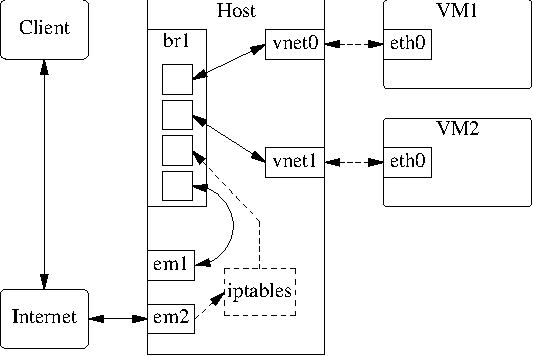
\includegraphics{graph/kvm_network.pdf}
\end{figure}


\section{qperf命令的使用}
\label{sec:qperfCmd}

我们在做网络服务器的时候,通常会很关心网络的带宽和延迟。因为我们的很多
协议都是request-response协议,延迟决定了最大的QPS,而带宽决定了最大的负
荷。 通常我们知道自己的网卡是什么型号,交换机什么型号,主机之间的物理距
离是多少,理论上是知道带宽和延迟是多少的。但是现实的情况是,真正的带宽
和延迟情况会有很多变数的,比如说网卡驱动,交换机跳数,丢包率,协议栈配
置,就实际速度而言,都很大的影响了数值的估算。 所以我们需要找到工具来实
际测量下。

SUSE11sp2发行版里面自带,方便安装,专业有效,能够针对TCP和RDMA进行带宽
和延迟的详细测试。

\begin{verbatim}
# zypper install -y qperf
\end{verbatim}

由于我们需要测试Infiniband的传输速率,在安装之前请先确认安装
了InfiniBand的相关包,比如librdmacm,libibverbs等。另外,也可以选择使用
源码包编译和安装qperf,但是需要注意,在安装之前也需要将infiniband相关的
包先安装上,否则RDMA的相关测试也将无法进行。

\begin{verbatim}
# zypper install -y librdmacm libibverbs
\end{verbatim}

\subsection{参数说明及示例}

qperf分为服务器端和客户端。客户端通过发送请求并获得响应来获得服务器端和
客户端之间的网络带宽以及延迟等信息。

\begin{tabular}{lp{20em}}
  \toprule
  参数名       & 参数说明 \\
  \midrule
  <server\_ip>	& 指定服务器的地址 \\
  time            & 指定网络测试时间。默认单位为秒,单位可以通过后缀为m,h,d指定为分钟,小时,天 \\
  conf	        & 测试输出中显示本地和远端服务器和操作系统配置 \\
  use\_bits\_per\_sec & 使用b(bit)而不是B(byte)来显示网络速度 \\
  precision 2	& 设置显示小数点后几位。这里设置为显示小数点后两位 \\
  verbose\_more	& 显示更详细的配置和状态信息 \\
  loop msg\_size:1:1025k:*2 	& loop表示对指定的指标值进行轮询。这里设置为对msg\_size轮询1,2,4,8…1024k,获得对应的测试结果,下次测试的指标值是上次测试指标值的*2倍 \\
  tcp\_bw	& 对tcp的带宽进行测试 \\
  tcp\_lat	& 对tcp的延迟进行测试 \\
  udp\_bw	& 对udp的带宽进行测试 \\
  udp\_lat	& 对udp的延迟进行测试 \\
  sdp\_bw	& 对sdp的延迟进行测试 \\
  sdp\_lat	& 对sdp的延迟进行测试 \\
\bottomrule
\end{tabular}

\section{iperf命令的使用}
\label{sec:iperfCmd}

iperf工具我们主要

首先到官网获取iperf工具,并把该工具放到合适的位置。
\begin{verbatim}
# wget https://iperf.fr/download/iperf_2.0.2/iperf_2.0.2-4_amd64
# chmod +x iperf_2.0.2-4_amd64
# mv iperf_2.0.2-4_amd64 /usr/bin/iperf
\end{verbatim}

\subsection{参数说明及示例}

\begin{tabular}{lp{25em}}
  \toprule
  参数名       & 参数说明 \\
  \midrule
  --server	& 以服务端模式运行 \\
  --udp	        & 指定测试UDP,默认为TCP带宽测试 \\
  --client <host>	& 以客户端模式运行,并连接<host> \\
  --bandwidth	& 指定测试中所使用的带宽,单位为[KM],默认为1Mbit/sec \\
  --time	        & 指定测试时间,单位为秒 \\
  --interval	& 指定多少时间间隔来报告测试结果,时间单位为秒 \\
  --format [kmKM]	& 指定报告的输出格式,单位分别为Kbits,Mbits,Kbytes,Mbytes \\
\bottomrule
\end{tabular}

\begin{enumerate}[itemsep=0pt,parsep=0pt]
\item 以太网UDP丢包率测试

\begin{verbatim}
A0304010:~ # iperf --server --udp 
A0305010:~ # iperf --udp --client 172.16.25.39 --interval 1 \
             --time 120 --bandwidth 900M
\end{verbatim}

\item InfiniBand网络UDP丢包率测试

\begin{verbatim}
# iperf --server --udp 
# iperf --udp --client 11.11.11.39 --interval 1 \
             --time 120 --bandwidth 1024M
\end{verbatim}

\item 如果不指定--udp选项,默认就是测试TCP带宽

\begin{verbatim}
A0304010:~ # iperf --server 
A0305010:~ # iperf --client 172.16.25.39  -f M
\end{verbatim}
\end{enumerate}

\section{vmstat命令的使用}
\label{sec:vmstatCmd}

Linux下vmstat输出释疑:

\begin{verbatim}
Vmstat
procs -----------memory---------- ---swap-- -----io---- --system-- ----cpu----
r b   swpd free buff cache          si so      bi bo      in cs    us sy id wa
0 0   100152 2436 97200 289740       0 1       34 45       99 33    0 0 99 0
\end{verbatim}

\begin{quote}
procs
r 列表示运行和等待cpu时间片的进程数,如果长期大于cpu个数,说明cpu不足,需要增加cpu。

b 列表示在等待资源的进程数,比如正在等待I/O、或者内存交换等。

memory
swpd 切换到内存交换区的内存数量(k表示)。如果swpd的值不为0,或者比较大,比如超过了100m,
     只要si、so的值长期为0,系统性能还是正常

free 当前的空闲页面列表中内存数量(k表示)

buff 作为buffer cache的内存数量,一般对块设备的读写才需要缓冲。

cache: 作为page cache的内存数量,一般作为文件系统的cache,如果cache较大,说明用到cache的
       文件较多,如果此时IO中bi比较小,说明文件系统效率比较好。

swap
si 由内存进入内存交换区数量。

so 由内存交换区进入内存数量。


IO
bi 从块设备读入数据的总量(读磁盘)(每秒kb)。

bo 块设备写入数据的总量(写磁盘)(每秒kb)


system 显示采集间隔内发生的中断数

in 列表示在某一时间间隔中观测到的每秒设备中断数。

cs 列表示每秒产生的上下文切换次数,如当cs比磁盘I/O和网络信息包速率高得多,都应进行进一步调查。



cpu 表示cpu的使用状态

us 列显示了用户方式下所花费 CPU 时间的百分比。us的值比较高时,说明用户进程消耗的cpu时间多,
   但是如果长期大于50\%,需要考虑优化用户的程序。

sy 列显示了内核进程所花费的cpu时间的百分比。这里us + sy的参考值为80\%,如果us+sy 大于
   80\%说明可能存在CPU不足。

wa 列显示了IO等待所占用的CPU时间的百分比。这里wa的参考值为30\%,如果wa超过30\%,说明IO等待严重,
   这可能是磁盘大量随机访问造成的,也可能磁盘或者磁盘访问控制器的带宽瓶颈造成的(主要是块操作)。

id 列显示了cpu处在空闲状态的时间百分比
\end{quote}


\section{iostat命令的使用}
\label{sec:iostatCmd}

\section{sar命令的使用}
\label{sec:sarCmd}

sar 命令行的常用格式:
\begin{verbatim}
sar [options] [-A] [-o file] t [n]
\end{verbatim}

在命令行中,n 和t 两个参数组合起来定义采样间隔和次数,t为采样间隔,是必
须有的参数,n为采样次数,是可选的,默认值是1,-o file表示将命令结果以二
进制格式存放在文件中,file 在此处不是关键字,是文件名。options 为命令行
选项,sar命令的选项很多,下面只列出常用选项:

\begin{table}[!htbp]
  \centering
  \begin{tabular}{ll}
    \toprule
    选项     & 说明 \\
    \midrule
    -A  & 所有报告的总和 \\
    -u  & CPU利用率 \\
    -v  & 进程、I节点、文件和锁表状态 \\
    -d  & 硬盘使用报告 \\
    -r  & 没有使用的内存页面和硬盘块 \\
    -g  & 串口I/O的情况(centos 5 中无此选项) \\
    -b  & 缓冲区使用情况 \\
    -a  & 文件读写情况 \\
    -c  & 系统调用情况 \\
    -R  & 进程的活动情况 \\
    -y  & 终端设备活动情况 \\
    -w  & 系统交换活动 \\
    \bottomrule
  \end{tabular}
  \caption{sar常用选项}
  \label{tab:sarOptions}
\end{table}

例一:使用命令行 sar -u t n

例如,每60秒采样一次,连续采样5次,观察CPU 的使用情况,并将采样结果以二
进制形式存入当前目录下的文件lavenliu中,需键入如下命令:

\begin{verbatim}
# sar -u -o lavenliu 60 5
SCO_SV   scosysv 3.2v5.0.5 i80386   10/01/2001
14:43:50   %usr   %sys  %wio    %idle(-u)
14:44:50   0     1    4      94
14:45:50   0     2    4      93
14:46:50   0     2    2      96
14:47:50   0     2    5      93
14:48:50   0     2    2      96
Average    0     2    4      94
\end{verbatim}

在显示内容包括:

\begin{verbatim}
%usr:CPU处在用户模式下的时间百分比。
%sys:CPU处在系统模式下的时间百分比。
%wio:CPU等待输入输出完成时间的百分比。
%idle:CPU空闲时间百分比。
\end{verbatim}

在所有的显示中,我们应主要注意\%wio和\%idle,\%wio的值过高,表示硬盘存
在I/O瓶颈,\%idle值高,表示CPU较空闲,如果\%idle值高但系统响应慢时,有
可能是CPU等待分配内存,此时应加大内存容量。\%idle值如果持续低于10,那么
系统的CPU处理能力相对较低,表明系统中最需要解决的资源是CPU。

如果要查看二进制文件lavenliu中的内容,则需键入如下sar命令:

\begin{verbatim}
# sar -u -f lavenliu
\end{verbatim}

可见,sar命令即可以实时采样,又可以对以往的采样结果进行查询。

例二:使用命行sar -v t n

例如,每30秒采样一次,连续采样5次,观察核心表的状态,需键入如下命令:

\begin{verbatim}
# sar -v 30 5
SCO_SV scosysv 3.2v5.0.5 i80386 10/01/2001
10:33:23 proc-sz ov inod-sz ov file-sz ov lock-sz   (-v)
10:33:53  305/ 321  0 1337/2764  0 1561/1706 0 40/ 128
10:34:23  308/ 321  0 1340/2764  0 1587/1706 0 37/ 128
10:34:53 305/ 321  0 1332/2764  0 1565/1706 0 36/ 128
10:35:23 308/ 321  0 1338/2764  0 1592/1706 0 37/ 128
10:35:53 308/ 321  0 1335/2764  0 1591/1706 0 37/ 128
\end{verbatim}

显示内容包括:

\begin{quote}
proc-sz:目前核心中正在使用或分配的进程表的表项数,由核心参数MAX-PROC控制。
inod-sz:目前核心中正在使用或分配的i节点表的表项数,由核心参数MAX-INODE控制
file-sz:目前核心中正在使用或分配的文件表的表项数,由核心参数MAX-FILE控制。
ov:     溢出出现的次数。
Lock-sz:目前核心中正在使用或分配的记录加锁的表项数,由核心参数MAX-FLCKRE控制。
\end{quote}

显示格式为: 实际使用表项/可以使用的表项数

显示内容表示,核心使用完全正常,三个表没有出现溢出现象,核心参数不需调
整,如果出现溢出时,要调整相应的核心参数,将对应的表项数加大。

例三:使用命行sar -d t n

例如,每30秒采样一次,连续采样5次,报告设备使用情况,需键入如下命令:
\begin{verbatim}
# sar -d 30 5
SCO_SV scosysv 3.2v5.0.5 i80386 10/01/2001
11:06:43 device %busy   avque   r+w/s  blks/s  avwait avserv (-d)
11:07:13 wd-0   1.47   2.75   4.67   14.73   5.50 3.14
11:07:43 wd-0   0.43   18.77   3.07   8.66   25.11 1.41
11:08:13 wd-0   0.77   2.78   2.77   7.26   4.94 2.77
11:08:43 wd-0   1.10   11.18   4.10   11.26   27.32 2.68
11:09:13 wd-0   1.97   21.78   5.86   34.06   69.66 3.35
Average wd-0   1.15   12.11   4.09   15.19   31.12 2.80
\end{verbatim}

显示内容包括:
\begin{verbatim}
device: sar命令正在监视的块设备的名字。
%busy: 设备忙时,传送请求所占时间的百分比。
avque: 队列站满时,未完成请求数量的平均值。
r+w/s: 每秒传送到设备或从设备传出的数据量。
blks/s: 每秒传送的块数,每块512字节。
avwait: 队列占满时传送请求等待队列空闲的平均时间。
avserv: 完成传送请求所需平均时间(毫秒)。
\end{verbatim}

在显示的内容中,wd-0是硬盘的名字,\%busy的值比较小,说明用于处理传送请求
的有效时间太少,文件系统效率不高,一般来讲,\%busy值高些,avque值低些,
文件系统的效率比较高,如果\%busy和avque值相对比较高,说明硬盘传输速度太
慢,需调整。

例四:使用命行sar -b t n

例如,每30秒采样一次,连续采样5次,报告缓冲区的使用情况,需键入如下命令:
\begin{verbatim}
# sar -b 30 5
SCO_SV scosysv 3.2v5.0.5 i80386 10/01/2001
14:54:59 bread/s lread/s %rcache bwrit/s lwrit/s %wcache pread/s pwrit/s (-b)
14:55:29 0  147  100  5  21  78   0   0
14:55:59 0  186  100  5  25  79   0   0
14:56:29 4  232   98  8  58  86   0   0
14:56:59 0  125  100  5  23  76   0   0
14:57:29 0   89  100  4  12  66   0   0
Average  1  156   99  5  28  80   0   0
\end{verbatim}

显示内容包括:
\begin{verbatim}
bread/s: 每秒从硬盘读入系统缓冲区buffer的物理块数。
lread/s: 平均每秒从系统buffer读出的逻辑块数。
%rcache: 在buffer cache中进行逻辑读的百分比。
bwrit/s: 平均每秒从系统buffer向磁盘所写的物理块数。
lwrit/s: 平均每秒写到系统buffer逻辑块数。
%wcache: 在buffer cache中进行逻辑读的百分比。
pread/s: 平均每秒请求物理读的次数。
pwrit/s: 平均每秒请求物理写的次数。
\end{verbatim}

在显示的内容中,最重要的是\%cache和\%wcache两列,它们的值体现着buffer的
使用效率,\%rcache的值小于90或者\%wcache的值低于65,应适当增加系
统buffer的数量,buffer数量由核心参数NBUF控制,使\%rcache达到90左
右,\%wcache达到80左右。但buffer参数值的多少影响I/O效率,增加buffer,应
在较大内存的情况下,否则系统效率反而得不到提高。

例五:使用命行sar -g t n
例如,每30秒采样一次,连续采样5次,报告串口I/O的操作情况,需键入如下命令:
\begin{verbatim}
# sar -g 30 5
SCO_SV scosysv 3.2v5.0.5 i80386  11/22/2001
17:07:03  ovsiohw/s  ovsiodma/s  ovclist/s (-g)
17:07:33   0.00   0.00   0.00
17:08:03   0.00   0.00   0.00
17:08:33   0.00   0.00   0.00
17:09:03   0.00   0.00   0.00
17:09:33   0.00   0.00   0.00
Average    0.00   0.00   0.00
\end{verbatim}

显示内容包括:
\begin{verbatim}
ovsiohw/s:每秒在串口I/O硬件出现的溢出。
ovsiodma/s:每秒在串口I/O的直接输入输出通道高速缓存出现的溢出。
ovclist/s :每秒字符队列出现的溢出。
\end{verbatim}

在显示的内容中,每一列的值都是零,表明在采样时间内,系统中没有发生串口
I/O溢出现象。

sar命令的用法很多,有时判断一个问题,需要几个sar命令结合起来使用,比如,
怀疑CPU存在瓶颈,可用sar -u 和sar -q来看,怀疑I/O存在瓶颈,可用sar -b、
sar -u和sar-d来看。

\section{ip命令的使用}
\label{sec:ipCmd}

\subsection{显示IP信息}



% 第三部分
\chapter{vim编辑器}
\label{sec:vimUsage}

当我们基本熟悉了操作系统的使用,是不是还少了什么件事?恭喜你猜对了,那
就是在系统里面编辑一些东西,我们总该留点什么东西吧,你说是不是呢?

传说中,蔚蓝的星球上流传着两大神器,一个是vi\footnote{vim是vi的升级版,
  一般认为vi\index{vi编辑器}既vim\index{vim编辑器},vim既vi。也可理解为
  vi为vim的一个别名。},一个是emacs。据说Vim是编辑器之神,而Emacs是神的
编辑器。追求独步天下的高手和低手们争着一睹它们的风采,可看到它们朴素单
薄的界面后,不禁心下怀疑:这就是神器吗?至有人生了轻视之心。

本文就向你展示如何使用vim,掌握它最基本的使用即可。作者刚开始使用vim的
时候,总是不由自主地想动动旁边的鼠标,大概用了两个晚上的时间才熟练的掌
握。Emacs可以根据自己兴趣看一看,作者使用了一年多的时间,也没觉得自己比
那些使用vim的家伙强\footnote{这里作者并不想卷入编辑器之战,不想得罪任何
  一方阵营,两种编辑器我都会使用,上班时用vi,不上班时用Emacs;如果真的
  得罪了某方阵营,请原谅我的无知。},我的vi用的比Emacs要熟练。嘿嘿!

\section{vim的几种模式}
\label{sec:vimMode}

vim有两种模式,一个为输入模式,一个为命令模式。在系统提示字
符(如\$、\#)下敲入vim filename,如果没有filename这个文件则会创建,若有则
打开。vim可以自动帮你载入所要编辑的文件或是开启一个新文件(如果该文件不
存在或缺少文件名)。进入vim后屏幕左方会出现波浪符号,凡是列首有该符号就
代表此列目前是空的。

如上所述,vim存在两种模式:指令模式和输入模式。在指令模式下输入的按键将
做为指令来处理:如输入i,vim即认为是在当前位置插入字符。而在输入模式
下,vim则把输入的按键当作插入的字符来处理。指令模式切换到输入模式只需键
入相应的输入命令即可(如a,A),而要从输入模式切换到指令模式,则需在输
入模式下键入ESC键,如果不晓得现在是处于什么模式,可以多按几次ESC,系统
如发出哔哔声就表示已处于指令模式下了。

\subsection{输入模式}

如何进入输入模式?下面列出几个进入插入模式的指令:

\begin{table}[htbp]
  \centering
    \caption{vim进入插入模式指令}
    \label{tab:vimInsertMode}
    \begin{tabular}{cl}
      \toprule
      指令  & 说明 \\
      \midrule
      i     & 在光标所在处进入插入模式 \\
      I     & 在当前行的行首进入插入模式 \\
      a     & 在光标的后面进入插入模式 \\
      A     & 在当前行的行尾进行插入模式 \\
      o     & 在光标所在行的下面新开一行 \\
      O     & 在光标所在行的上面新开一行 \\
      s     & 删除光标所在字符并进入插入模式 \\
      S     & 删除光标所在行并进入输入模式 \\
      \bottomrule
    \end{tabular}
\end{table}

大家注意到了没有,大写与小写分别控制反向与正向。如何退出呢?在插入模式
下,需要按下键盘的ESC键,进入命令模式,再从命令模式下,输入”:wq“即可
退出。wq的意思是保存并退出,如果不想保存,只需输入”:q“即可。如果修改
后,发现改错了文件,并不想保存了,在命令模式下输入”:q!“即可,加
上”!“作用是强制退出不保存,其实也可以强制保存并退出的,该怎么输入?想
想看。

\subsection{命令模式}

在刚打开vim编辑器时,这时所处的模式是命令模式;从输入模式返回到命令模式,
只需要按下键盘上的ESC键即可返回到命令模式。下面介绍几组很实用的指令,主
要涉及删除、复制及粘贴的指令,还有几个控制光标移动的指令。

光标方向控制:

\begin{table}[htbp]
  \centering
    \caption{vim方向控制键}
    \label{tab:vimDirection}
    \begin{tabular}{cl}
      \toprule
      指令  & 说明 \\
      \midrule
      h  & 光标向前移动 \\
      j  & 光标向下移动 \\
      k  & 光标向上移动 \\
      l  & 光标想后移动 \\
      G  & 按下shift与G组合,则跳到文件末尾 \\
      gg & 连续按两次G,跳到文件的首行 \\
      \bottomrule
    \end{tabular}
\end{table}

撤销指令:

\begin{table}[htbp]
  \begin{center}
    \caption{vim撤销指令按键}
    \label{tab:vimUndoKey}
    \begin{tabular}{cl}
      \hline
      指令  & 说明 \\
      \hline
      u    & 按一次,撤销上一次的操作,按两次呢?哈哈 \\
      \hline
      :e!  & 直接回到了刚打开时的状态 \\
      \hline
    \end{tabular}
  \end{center}
\end{table}

删除指令:

\begin{table}[htbp]
  \begin{center}
    \caption{vim删除指令按键}
    \label{tab:vimDeleteKey}
    \begin{tabular}{cl}
      \hline
      指令  & 说明 \\
      \hline
      dd    & 删除当前光标所在行 \\
      \hline
      ndd   & 删除当前光标所在行及以下行共n行,其中n为数字 \\
      \hline
    \end{tabular}
  \end{center}
\end{table}

\subsection{vim的其他一些指令}

\section{vim的一些小技巧}

\begin{verbatim}
# 打开文件定位到指定行
vim +24 file       

# 打开多个文件	
vim file1 file2    

# 垂直分屏
vim -O file1 file2 

# 水平分屏
vim -o file1 file2 

# 上下分割打开新文件
sp filename       

# 左右分割打开新文件 
vsp filename      


# 多个文件间操作  大写W  
# 操作: 
#   关闭当前窗口c  
#   屏幕高度一样=  
#   增加高度+  
#   移动光标所在屏 右l 左h 上k 下j 中h  下一个w  
Ctrl+W [操作] 

# 编辑下一个文件
:n            

# 编辑下二个文件     
:2n           

# 编辑前一个文件
:N            

# 回到首文件
:rew               

# 打开行号
:set nu            

# 取消行号
:set nonu          

# 跳转到200
200G               

# 取消高亮
:nohl              

# 设置自动缩进
:set autoindent    

# 查看文本格式
:set ff            

# 改为unix格式
:set binary        

# 向前翻页
ctrl+ U            

# 向后翻页
ctrl+ D            

# 全部替换	
% s/字符1/字符2/g   

# 文档加密
X                  
\end{verbatim}

\section{vim复制粘贴及剪切板}

复制粘贴指令:

\begin{table}[!h]
  \begin{center}
    \begin{tabular}{cl}
      \hline
      指令  & 说明 \\
      \hline
      yy    & 复制当前光标所在行 \\
      \hline
      nyy   & 复制当前行及以下行共n行,n为数字 \\
      \hline
      p     & 将复制的内容粘贴到当前光标的下面一行,可以与数字一起使用,如np \\
      \hline
      P     & 将复制的内容粘贴到当前光标的上面一行,可以与数字一起使用,如nP \\
      \hline
    \end{tabular}
  \end{center}
\end{table}

vim有12个粘贴板,分别是0、1、2、...、9、a、“、+;
用:reg命令可以查看各个粘贴板里的内容。效果如图所示:

\begin{figure}[htbp]
  \begin{center}
    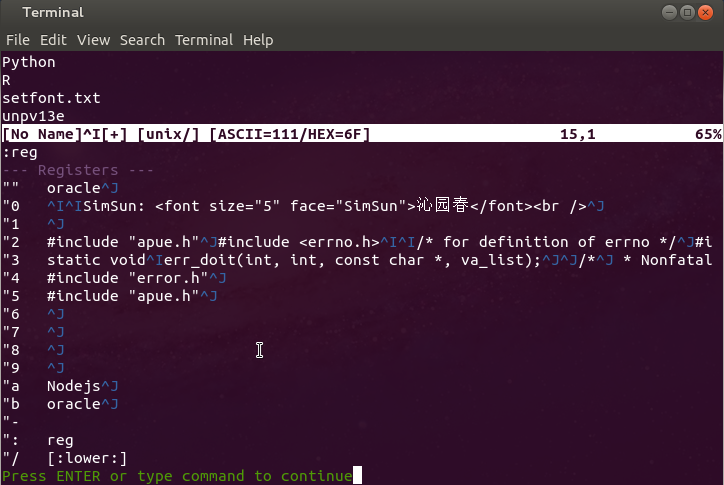
\includegraphics[width=.75\textwidth]{img/vimregister.png}
  \end{center}
  \caption{vim粘贴板一览}
  \label{fig:vimClipBoard}
\end{figure}

在vim中简单用y只是复制到"(双引号)粘贴板里,同样用p粘贴的内容也是这个
粘贴板里的内容;要将vim的内容复制到某个粘贴板,需要退出编辑模式,进入
正常模式后,选择要将复制的内容,然后按"Ny(注意带引号)完成复制,其中N为
粘贴板号(注意是按一下双引号后按粘贴板号再按y),比如要把内容复制到粘贴
板a,选中内容后按"ay就可以了。

有两点需要说明一下:"号粘贴板(临时粘贴板)比较特殊,直接按y就复制到这个
粘贴板中了,直接按p就粘贴这个粘贴板中的内容;+号粘贴板是系统粘贴板,
用"+y将内容复制到该粘贴板后可以使用Ctrl+V将其粘贴到其他文
档(如firefox、gedit)中,同理,要把在其他地方用Ctrl+C或右键复制的内容复
制到vim中,需要在正常模式下按"+p;

\section{vim配置文件}

我相信,每个有想法的家伙肯定不会满足默认的配置,他们总喜欢捣鼓。这个时
候我们就可以定制自己的编辑器了,以满足我们日常编辑的需求。Emacs的定制配
置更是令人蛋疼,诸多选项、诸多值……。作者曾经也是为此事而蛋疼不已,只是
学会了在Emacs里配置\LaTeX\index{\LaTeX}的一些配置项,其它神马的,作者是
一窍不通。

令人蛋疼的事就不多说,我比较喜欢简洁的配置。本人也不会开发,一些简单的
配置就能满足日常需要了,再说这个东东用的也不多。其它高大上的配置东东对
我来说也是浮云。下面是我常用的vim的配置文件\footnote{我的配置文件基本上
  是随身携带或者上传到云盘,然后把配置文件放到公司服务器上自己的家目录},
配置如下:

\begin{verbatim}
[root@iLiuc ~]# cat ~/.vimrc
set nocompatible
filetype indent on
filetype plugin on
set tabstop=4
set shiftwidth=4
set autoindent
set cindent
set smartindent
set hlsearch
syntax enable
set dict=/usr/share/dict/words

if has('statusline')
    set laststatus=2

    " Broken down into easily includeable segments
    set statusline=%<%f\            " Filename
    set statusline+=%w%h%m%r        " Options
    set statusline+=\ [%{&ff}/%Y]   " filetype

    " ASCII/Hexadecimal value of under current cursor
    set statusline+=\ [ASCII=\%03.3b/HEX=\%02.2B]

    " Right aligned file nav info
    set statusline+=%=%-14.(%l,%c%V%)\ %p%%
endif
\end{verbatim}

效果如下:

\begin{figure}[htbp]
  \centering
  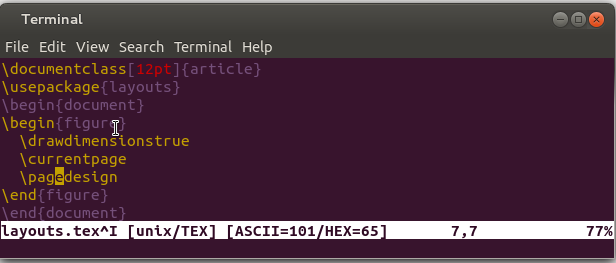
\includegraphics[width=.75\textwidth]{img/vimrc.png}
  \caption{vim配置文件效果}
  \label{fig:vimConf}
\end{figure}

就先写这么多吧,如果我要再写下去,就不止这么多。
呵呵!只不过是两年没用认真的使用了。呵呵!vim的使用就介绍这么多,我想仅
仅学会这些就能让初学者的效率有很大的提高,但还不够高,这里并没有介绍正
则表达式等。


% 第四部分
\chapter{Bash脚本}
\label{sec:shellScript}
\index{bash}

无聊地重复一件事确实惹人厌!当然了,数次重复一些命令是不是也是很不爽的
一件事呢?如果是请跟随我往下看。当我们熟悉了操作系统后,以期望有更好的
提高,那就是写脚本了。

\section{正则表达式}

Regular expression\index{Regular Expression} (abbreviated regex or
regexp) is a sequence of characters that forms a search pattern,
mainly for use in pattern matching with strings, or string matching,
i.e. "find and replace"\-like operations.

正则表达式就是由一系列特殊字符组成的字符串, 其中每个特殊字符都被称为元
字符, 这些元字符并不表示为它们字面上的含义, 而会被解释为一些特定的含义.
具个例子, 比如引用符号, 可能就是表示某人的演讲内容, 同上, 也可能表示为
我们下面将要讲到的符号的元-含义. 正则表达式其实是由普通字符和元字符共同
组成的集合, 这个集合用来匹配(或指定)模式.

一个正则表达式会包含下列一项或多项:

\begin{enumerate}[itemsep=0pt,parsep=0pt]
\item 一个字符集. 这里所指的字符集只包含普通字符, 这些字符只表示它们的
  字面含义. 正则表达式的最简单形式就是只包含字符集, 而不包含元字符.
\item 锚. 锚指定了正则表达式所要匹配的文本在文本行中所处的位置. 比如,
  \^, 和\$就是锚.
\item 修饰符. 它们扩大或缩小(修改)了正则表达式匹配文本的范围. 修饰符包
  含星号, 括号, 和反斜杠.
\end{enumerate}

\subsection{正则表达式语法}

\subsection{一些实例}


\section{awk}
\label{sec:awk}

如果要格式化报文或从一个大的文本文件中抽取数据包,那么awk可以完成这些任
务。它在文本浏览和数据的熟练使用上性能优异。与其它大多数Unix/Linux命令
不同的是,从名字上看,我们一眼看不出awk\index{awk}的功能:它既不是具有独立意义的英
文单词,也不是几个相关单词的缩写。事实上,awk是三个人名的缩写,他们是:
Aho、(Peter) Weinberg和(Brain)Kernighan。正是这三个家伙创造了awk,一个
优秀的样式扫描与处理工具。本章只介绍Gnu的awk版本gawk,其他awk版本不做介
绍。

awk的工作流程:
\begin{figure}[!htbp]
  \centering
  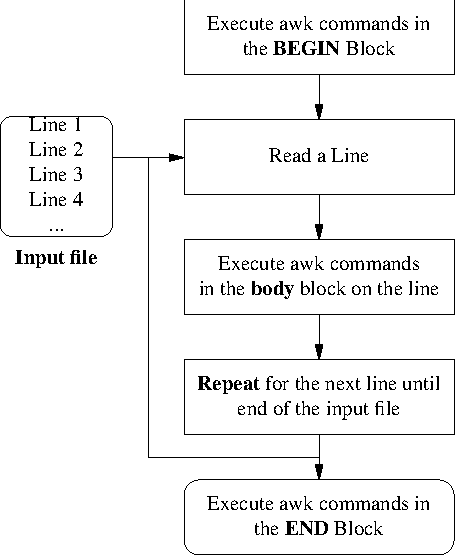
\includegraphics[width=.5\textwidth]{graph/awk_workflow.pdf}
  \caption{awk工作流程}
  \label{fig:awk_workflow}
\end{figure}

\subsection{初步使用}
\label{subsec:FirstAwk}

假如我们有文件employee.txt,内容如下:

\begin{verbatim}
Beth	4.00	0
Dan	3.75	0
Kathy	4.00	10
Mark	5.00	20
Mary	6.50	22
Susie	6.25	18
\end{verbatim}

第一列表示员工姓名,第二列表示每小时加班所得的人民币,第三列为加班多少
小时。我们现在就来打印出那些加班大于0个小时的员工及其加班费,在命令行只
需执行这样一行命令即可:

\begin{verbatim}
# awk '$3 > 0 { print $1, $2 * $3 }' employee.txt
\end{verbatim}

我们会得到这样的输出:

\begin{verbatim}
Kathy 40
Mark 100
Mary 143
Susie 112.5
\end{verbatim}

上面的命令告诉系统运行awk,使用单引号里的程序,并从employee.txt文件里获
得自己的数据。单引号里的部分完全就是awk程序。它包含了单个的
pattern-action(模式-动作)语句。动作\$3 >  0,匹配输入的每一行的第三列
或域,如果该列大于0,然后就执行下面的动作

\begin{verbatim}
{ print $1, $2 * $3 }
\end{verbatim}

对于每匹配到的行,就会打印第一个域并同时计算第二个域与第三个域的乘积。

如果我们想看看哪个家伙这个月没有加班,可以使用下面的命令:

\begin{verbatim}
# awk '$3 == 0 { print $1 }' employee.txt
\end{verbatim}

这里的模式,\$3 == 0,将会匹配每一输入行的第三个域,如果等于0,就会执行
下面的动作

\begin{verbatim}
{ print $1 }
\end{verbatim}

打印第一个域。

\subsection{awk程序结构}

awk的基本操作是对输入的行做逐一扫描,搜索这些行中匹配到的任意模式,然后
执行相应的动作。然后下一行被读进来并从头开始匹配到行末,直到输入文件的
所有行被读进来。就\$3 > 0来说,当满足时,说明该条件为真。

在上面的例子中,只有一个模式和动作,可以称为单pattern-action语句;对于
每一行,匹配到第三个字段等于0时,第一个字段将会被打印。

另外,模式和动作并不总是成对出现的,就是说,在pattern-action语句中,可
能只有模式或者只有动作。如果一个pattern没有相应的action,例如,

\begin{verbatim}
$3 == 0
\end{verbatim}

然后,每一被匹配的行都将会被打印,

\begin{verbatim}
Beth    4.00    0
Dan     3.75    0
\end{verbatim}

如果一个action没有pattern时,例如,

\begin{verbatim}
{ print $1 }
\end{verbatim}

此时,将会打印每一行的第一个域。由上可知,patterns和actions都是可选的。
actions使用大括号括起来以与patterns区分。

\subsection{BEGIN与END}

特殊的BEGIN模式在第一个输入文件的第一行被匹配,而END则是在最后一个文件的最后被处理后匹配。
下面的程序将会打印一个头部:

\begin{verbatim}
BEGIN { print "NAME     RATE    HOURS"; print "" }
      { print }
\end{verbatim}

我们将会得到这样的输出:

\begin{verbatim}
NAME     RATE   HOURS

Beth     4.00   0
Dan      3.75   0
Kathy    4.00   10
Mark     5.00   20
Mary     6.50   22
Susie    6.25   18
\end{verbatim}

我们可以在一行同时输入多条语句,这些语句之间需要用分号分开。注意
到,\textit{print ""}意思是打印一个空行,它与print不一样,仅仅一
个print语句将打印整行。

\subsection{域和记录}
\label{subsec:FieldRecordAwk}

awk执行时,其浏览域标记为\$1,\$2,...\$n。这种方法称为域标识。使用这些
域标识将更容易对域进一步处理。

\subsection{内置变量}

awk有一些内置的变量,变量如下:

\begin{table}[hbtp]
  \begin{center}
    \begin{tabular}{ll}
      \hline
      变量     & 说明 \\
      \hline
      ARGC        & 命令行中参数的个数 \\
      \hline
      ARGV        & 包含命令行参数的数组 \\
      \hline
      CONVFMT     & 用于数字的字符串转换格式(默认格式为\%.6g) \\
      \hline
      ENVIRON     & 环境变量的关联数组 \\
      \hline
      FILENAME    & 当前文件名 \\
      \hline
      NR          & 当前记录的个数(当前的行号) \\
      \hline
      FNR         &  当前记录的个数(仅为当前文件,而非全部输入文件) \\
      \hline
      FS          & 字段分割符(默认为空格) \\
      \hline
      NF          & 当前记录中的字段个数 \\
      \hline 
      OFMT        & 数字的输出格式(默认格式为\%.6g) \\
      \hline
      OFS         & 输出字符的分割符(默认为空格) \\
      \hline
      ORS         & 输出记录分割符(默认为换行) \\
      \hline
    \end{tabular}
  \end{center}
\end{table}

\subsection{One-liners awk程序}

这一节介绍几个很有用的、短小精悍的awk程序。

\begin{enumerate}
\item 打印输入文件的总行数
\item 打印指定的行
\item 打印输入行的最后一个字段
\item 打印最后一行的最后一个字段
\item 打印每一输入行并擦除第二个字段
\end{enumerate}

\subsection{条件和循环}

这一节包含了一些基本的编程结构。它覆盖了awk程序设计语言中的所有控制结构。
在awk中,这些条件和循环的语法用起来比较简单。实际上,awk中的条件和循环
结构的语法借鉴C语言。因此,通过学习awk,我们也同样在学习C语言。

\subsection{if-else语句}

awk提供一个\textit{if-else}语句,这些语句只能用在actions中。下面的这个
程序使用的还是\ref{sec:FirstAwk}节的例子。在这个例子中,我们会计算那些
每小时加班费大于6块的家伙,他们的总加班费及平均加班费。

\begin{verbatim}
# cat progfile
$2 > 6 { n = n + 1; pay = pay + $2 * $3 }
END    { if (n > 0)
            print n, "employees, total pay is", pay,
                     "average pay is", pay / n
         else
            print "no employees are paid more than Y6/hour"
}

# awk -f progfile employee.txt
\end{verbatim}

我们将会得到下面的输出结果:

\begin{verbatim}
  2 employees, total pay is 255.5 average pay is 127.75
\end{verbatim}

\subsection{while循环}
\label{subsec:WhileLoop}

while语句有一个condition和一个body。当condition为真时,body中的语句将被重复执行。我们使用下面的
程序计算这样的一个公式$ value = amount(1+rate)^{years} $

\begin{verbatim}
  # cat interest1 
  # interest1 - compute compound interest
  #   formula: value = amount(1+rate)^years
  #   input: amount rate years
  #   output: compounded value at the end of each year
  
  {  i = 1
    while (i <= $3) {
      printf("\t%.2f\n", $1 * (1 + $2) ^ i)
      i = i + 1
    }
  }
\end{verbatim}

如何执行该程序?看操作,

\begin{verbatim}
  # awk -f interest1 <- 回车
  1000 .06 5 <- 输入三组数字后,回车
  1060.00
  1123.60
  1191.02
  1262.48
  1338.23
\end{verbatim}

\subsection{for循环}
\label{subsec:ForLoop}

我们使用for语句改写第\ref{subsec:WhileLoop}节的while程序。如下:

\begin{verbatim}
  # cat interest2
  # interest2 - compute compound interest
  #   formula: value = amount(1+rate)^years
  #   input: amount rate years
  #   output: compounded value at the end of each year
  
  {  for (i = 1; i <= $3; i = i + 1)
    printf("\t%.2f\n", $1 * (1 + $2) ^ i)
  }
\end{verbatim}

\subsection{do循环}

\subsection{影响流控制的语句}

\subsection{数组}

数组是可以用来存储一组数据的变量。通常这些数据之间具有某种关系。数组中
的每一个元素通过它们在数组中的下标来访问。每个下标用方括号括起来。下面
的语句表示为数组中的一个元素赋值。

\begin{verbatim}
  array[subscript] = value
\end{verbatim}

在awk中不必指明数组的大小,只需要为数组指定标示符。向数组元素赋值比较容
易。例如,下面的例子中为数组hr的一个元素指定了一个字符串“laven”。

\begin{verbatim}
  hr[1] = "laven"
\end{verbatim}

这个数组元素的下标是“1”,下面的语句将打印字符串“laven”。

\begin{verbatim}
  print hr[1]
\end{verbatim}

当然,我们可以用循环向数组中写入或取出元素。例如,如果数组hr有10个元素,
可以使用下面的循环来打印每个元素:

\begin{verbatim}
  hr_count = 10
  for (x = 1; x <= hr_count; ++x)
  print hr[x]
\end{verbatim}

我们来看一个例子,依然使用第\ref{sec:FirstAwk}节中的输入文件,让employee.txt文件反序输出,

\begin{verbatim}
# cat reverse
# reverse - print input in reverse order by line
{ line[NR] = $0 } # remember each input line
END  { i = NR          # print lines in reverse order
  while (i > 0) {
    print line[i]
    i = i - 1
  }
}
  
# awk -f reverse employee.txt
Susie    6.25   18
Mary     6.50   22
Mark     5.00   20
Kathy    4.00   10
Dan      3.75   0
Beth     4.00   0
\end{verbatim}

\subsection{表达式}

\begin{verbatim}
# cat awk_file 
gold     1    1986  USA                 American Eagle
gold     1    1908  Austria-Hungary     Franz Josef 100 Korona
silver  10    1981  USA                 ingot
gold     1    1984  Switzerland         ingot
gold     1    1979  RSA                 Krugerrand
gold     0.5  1981  RSA                 Krugerrand
gold     0.1  1986  PRC                 Panda
silver   1    1986  USA                 Liberty dollar
gold     0.25 1986  USA                 Liberty 5-dollar piece
silver   0.5  1986  USA                 Liberty 50-cent piece
silver   1    1987  USA                 Constitution dollar
gold     0.25 1987  USA                 Constitution 5-dollar piece
gold     1    1988  Canada              Maple Leaf
\end{verbatim}

\begin{verbatim}
# This is an awk program that summarizes a coin collection.
#
/gold/    { num_gold++; wt_gold += $2 }    # Get weight of gold.
/silver/  { num_silver++; wt_silver += $2 }# Get weight of silver.
END { val_gold = 485 * wt_gold;            # Compute value of gold.
    val_silver = 16 * wt_silver;         # Compute value of silver.
    total = val_gold + val_silver;
    print "Summary data for coin collection:";  # Print results.
    printf ("\n");
    printf ("   Gold pieces:                 %2d\n", num_gold);
    printf ("   Weight of gold pieces:       %5.2f\n", wt_gold);
    printf ("   Value of gold pieces:        %7.2f\n",val_gold);
    printf ("\n");
    printf ("   Silver pieces:               %2d\n", num_silver);
    printf ("   Weight of silver pieces:     %5.2f\n", wt_silver);
    printf ("   Value of silver pieces:      %7.2f\n",val_silver);
    printf ("\n");
    printf ("   Total number of pieces:      %2d\n", NR);
    printf ("   Value of collection:         %7.2f\n", total);
}
\end{verbatim}

\begin{verbatim}
[root@unionpay bash]# awk -f myawk awk_file 
Summary data for coin collection:

   Gold pieces:                    9
   Weight of gold pieces:          6.10
   Value of gold pieces:        2958.50

   Silver pieces:                  4
   Weight of silver pieces:       12.50
   Value of silver pieces:       200.00

   Total number of pieces:        13
   Value of collection:         3158.50
\end{verbatim}

\subsection{函数}

\subsection{总结}


\section{sed}
\label{sec:sed}

Sed\index{sed}是一个超级流式编辑器。
picture a stream flowing through a pipe. Okay, you can't see a stream
if it's inside a pipe. That's what I get for attempting a flowing
analogy. You want literature, read James Joyce.

Anyhow, sed is a marvelous utility. Unfortunately, most people never
learn its real power. The language is very simple, but the
documentation is terrible. The Solaris on-line manual pages for sed
are five pages long, and two of those pages describe the 34 different
errors you can get. A program that spends as much space documenting
the errors than it does documenting the language has a serious
learning curve.

Do not fret! It is not your fault you don't understand sed. I will
cover sed completely. But I will describe the features in the order
that I learned them. I didn't learn everything at once. You don't need
to either.

sed的工作流程:
\begin{figure}[!htbp]
  \centering
  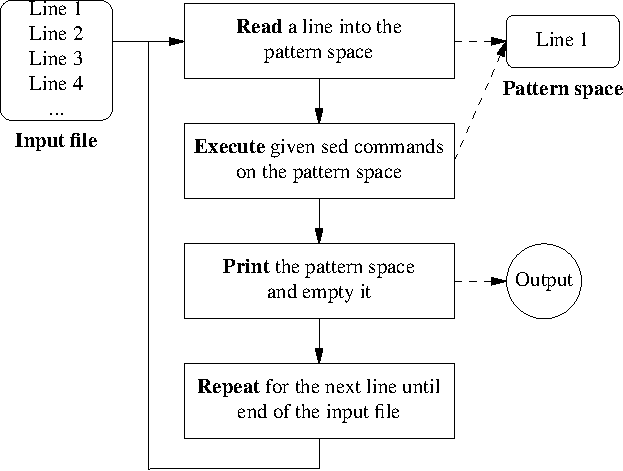
\includegraphics[width=.65\textwidth]{graph/sed_workflow.pdf}
    \caption{sed工作流程}
  \label{fig:sed_workflow}
\end{figure}

命令列表:

\begin{tabular}{lp{25em}}
\toprule
命令       & 说明 \\
\midrule
a          & 在当前行后面追加文本 \\
b label    & 分支到脚本中带有标号的地方,如果标号不存在就分支到脚本的末尾 \\
c          & 用新的文本改变或者替代本行的文本 \\
d          & 从模板块(Pattern space)位置删除行 \\
D          & 删除模板块的第一行 \\
i          & 在当前行上面插入文本 \\
h          & 拷贝模板块的内容到内存中的缓冲区 \\
H          & 追加模板块的内容到内存中的缓冲区 \\
g          & 获得内存缓冲区的内容,并替代当前模板块中的文本 \\
G          & 获得内存缓冲区的内容,并追加到当前模板块文本的后面 \\
l          & 列表不能打印字符的清单 \\
n          & 读取下一个输入行,用下一个命令处理新的行而不是用第一个命令 \\
N          & 追加下一个输入行到模板块后面并在二者之间嵌入一个新的行,改变当前行的号码 \\
p          & 打印模板块的行 \\
P          & 打印模板块的第一行 \\
q          & 退出 sed \\
r file     & 从file中读行 \\
t label    & if分支,从最后一行开始,条件一旦被满足或者T命令或者t命令, 将导致分支到带有标号的命令处,或者到脚本的末尾 \\
T label    & 错误分支,从最后一行开始,一旦发生错误或者T命令或者t命令, 将导致分支到带有标号的命令处,或者到脚本的末尾 \\
w file     & 写并追模板块到file末尾 \\
W file     & 写并追模板块的第一行到file末尾 \\
!          & 表示后面的命令对所有没有被选定的行发生作用 \\
s/re/string/ & 用string替换正则表达式re \\
=          & 打印当前行号码 \\
注释command & 把注释扩展到下一个换行符以前替换标记 \\
g           & 行内全面替换 \\
p           & 打印行 \\
w           & 把行写入一个文件 \\
x           & 互换模板块中的文本和缓冲区中的文本 \\
y           & 把一个字符翻译为另外的字符(但是不能用于正则表达式) \\
\bottomrule
\end{tabular}

一些选项:

\begin{tabular}{l|lp{20em}}
\hline
-e command             & 允许多点编辑 \\
\hline
--expression=command   & 同上 \\
\hline
-h,--help              & 打印命令行选项摘要,并显示 bug 列表的地址 \\
\hline
-n,--quiet,--silent    & 取消默认输出 \\
\hline
-f,                    & 引导 sed 脚本文件名 \\
\hline
--filr=script-file     & 同上 \\
\hline
-V,--version           & 打印版本和版权信息\\
\hline
\end{tabular}

\subsection{匹配}
\label{sec:sedPattern}

\subsection{变量定义}
\label{subsec:sedVariableDef}

\subsection{特殊变量}
\label{subsec:sedSpecialVariable}

\subsection{数组}
\label{subsec:sedArray}

\subsection{删除}
\label{subsec:sedDelete}

删除(d)编辑命令采用一个地址,如果行匹配这个地址就删除模式空间的内容。
删除命令(d)还是一个可以改变脚本中的控制流的命令。这是因为一旦执行这个
命令,那么在“空的”模式空间中就不会再有命令执行。删除命令(d)会导致读取
新输入行,而编辑脚本则从头开始新的一轮。重要的是,如果某行匹配这个地址,
那么就删除整个行,而不只是删除行中匹配的部分。

\subsection{替换}
 
Sed有众多命令,但经常被用到的就是最基本的替换命令“s”了, 替换命令有四部
分组成,如下表所示:

\begin{table}[h]
\centering
\begin{tabular}{l|l}
\hline
s	     & 所使用的命令是替换命令 \\
\hline
/../../	 & 所使用的分隔符,可以自行改变,不过三个符号要一致 \\
\hline
old	     & 这是将要被替换的字符串或正则表达式 \\
\hline
new	     & 这是替换后的字符串 \\
\hline
\end{tabular}
\end{table}

sed s/day/night/ <old >new

eg: sed 's/local/host/[g]' /etc/hosts
 
Or another way (for Unix beginners), 

sed s/day/night/ old >new
 
我们也可以如下这样写,

\small{
\begin{verbatim}
echo day | sed s/day/night/ 
\end{verbatim}
}
\normalsize

将会输出“night”。

我们在这里并没有使用引号把这些参数给引用起来,也能得出想要的结果,因为
这个例子是不需要它们的,嘿嘿!然而,在使用过程中出现了原字符,这时候引
号是必须要的。如果我们不确定何时要使用引号,那么,最好的习惯就是“每用
必带”引号即可,不用纠结那么多。

sed 's/day/night/' <old >new

I must emphasize that the sed editor changes exactly what you tell it
to. So if you executed
 
\begin{verbatim}
eg: # echo Sunday | sed 's/day/night/'
output: Sunnight
\end{verbatim}
 
This would output the word "Sunnight" bacause sed found the string
"day" in the input.
 
The search pattern is on the left hand side and the replacement string
is on the right hand side.
 
We've covered quoting and regular expressions. That's 90\% of the
effort needed to learn the substitute command. To put it another way,
you already know how to handle 90\% of the most frequent uses of
sed. There are a ... few fine points that an future sed expert should
know about. (You just finished section 1. There's only 63 more
sections to cover. :-) Oh. And you may want to bookmark this page,
.... just in case you don't finish.

\subsection{追加、插入和更改}
\label{subsec:appendInsertChange}

追加(a)、更改(c)、插入(i)编辑命令提供了类似于vi交互式编辑器的编辑功能。

追加命令(a)将文本放置在当前行之后。更改命令(c)用所指定的文本取代模
式空间的内容。插入命令(i)将所提供的文本放置在模式空间的当前行之前。这
些命令中的每一个都要求后面跟一个反斜杠用于转义第一个行尾。如要输入多行
文本,每个连续的行都必须用反斜杠结束,最后一行除外。而且,如果文本包含
一个字面含义的反斜杠,要再添加一个反斜杠来转义它。

\subsection{模式空间和保留空间}
\label{subsec:patternSpace}

\subsection{流控制}
\label{subsec:flowControl}

\subsection{地址范围}
\label{subsec:addrSpace}

\subsection{调用外部变量}
\label{subsec:callExternalVariable}

\subsection{总结}
\label{subsec:summary}



\section{语法介绍}

\subsection{变量定义}

\subsection{特殊变量}

在脚本里有以下几个特殊的变量,如下

\begin{table}[htbp]
  \centering
  \caption{特殊变量的含义}
  \label{tab:specialVariables}
  \begin{tabular}{cl}
    \toprule
    变量  & 说明 \\
    \midrule
    \$0   & 代表该脚本的名字 \\
    \$n   & 代表该程序的第n\footnote{如果参数超过10个,则使用\$n就不合适了,需要使用\$\{n\}的形式。}个参数值,n=1..9 \\
    \$*   & 代表该脚本的所有参数 \\
    \$\#  & 代表该脚本的参数个数 \\
    \$\$  & 代表该脚本的PID \\
    \$!   & 代表上一个指令的PID \\
    \$?   & 代表上一个指令的返回值 \\
    \bottomrule
  \end{tabular}
\end{table}

\subsection{变量赋值和替换}

\subsection{本地变量与全局变量}

\subsection{引用变量}

\subsection{数组}

Bash只支持一维数组,但参数个数没有限制。

数组赋值:

\begin{verbatim}
1. array=(var1 var2 var3 ... varN)
2. array=([0]=var1 [1]=var2 [2]=var3 ... [n]=varN)
3. array[0]=var1
   array[1]=var2
   array[2]=var3
   ...
   array[N]=varN
\end{verbatim}

\begin{verbatim}
  declare -

  MYARRAY=([0]=tom [1]=laven [2]=liu [5]=jim)
  
  数组的元素的长度:
  ${#MYARRAY} 指的是数组MYARRAY的第0个元素的长度,与
  ${#MYARRAY[0]} 等价
  ${#MYARRAY[n]} 是第n+1个元素,

  数组的元素个数:
  ${#MYARRAY[*]}
  ${#MYARRAY[@]}
\end{verbatim}
  一个例子,随机生成10个整型元素的的数组,并找出该数组中的最大值。
  \begin{lstlisting}
  #!/bin/bash
  #
  for i in {0..9}
  do
  ARRAY[$i]=$RANDOM
  echo -n "${ARRAY[$i]} "
  sleep 1
  done

  echo

  declare -i MAX=${ARRAY[0]}
  INDEX=$[${#ARRAY[*]-1}]
  for i in `seq 1 $INDEX`
  do
      if [ $MAX -lt ${ARRAY[$i]} ] ; then
          MAX=${ARRAY[$i]}
      fi
  done

  echo ${MAX}
  \end{lstlisting}

\subsection{特殊字符}

\section{基本流程}

Bash与其他编程语言一样,也有自己的程序处理逻辑。接下来的这个章节主要介
绍Bash的脚本几种基本流程。

\subsection{if结构}

先看一下bash的man page是如何定义if结构的,

\begin{figure}[!htbp]
  \centering
  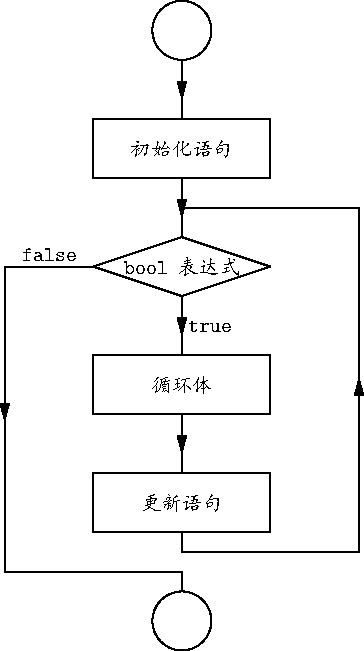
\includegraphics{graph/for.pdf}
    \caption{for工作流程}
  \label{fig:for_workflow}
\end{figure}

\begin{verbatim}
if list; then 
    list; 
[ elif list; then list; ] 
... 
[ else list; ] 
fi
\end{verbatim}

当\emph{if list}执行成功并且返回状态是0时,相应的\emph{then list}就会被
执行;否则,\emph{elif list}执行,且返回状态为0时,相应的\emph{then
  list}就会被执行;之后命令执行结束。如果前面的\emph{if list}及
\emph{elif list}都不能成功执行,那么将执行最后一个\emph{else list}语句。
返回状态就是上一条命令执行成功与否,执行成功就返回0,不成功返回非0。不
成功的原因有很多,成功返回就一个。

一个示例:

\lstinputlisting[aboveskip=5pt,belowskip=5pt,language=bash]{src/shell01.sh}

\subsection{for结构}

\begin{figure}[!htbp]
  \centering
  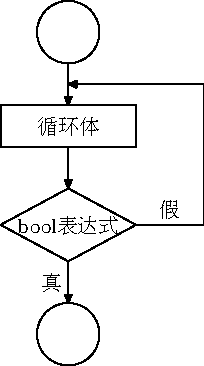
\includegraphics{graph/do-1.pdf}
    \caption{do工作流程}
  \label{fig:do_workflow}
\end{figure}

\begin{lstlisting}
#!/bin/sh

# numberlines - A simple alternative to cat -n, etc.

for filename
do
    linecount="1"
    while read line
    do
        echo "${linecount}: $line"
        linecount="$(($linecount + 1))"
    done < $filename
done
exit 0
\end{lstlisting}

\subsection{while结构}

\begin{figure}[!htbp]
  \centering
  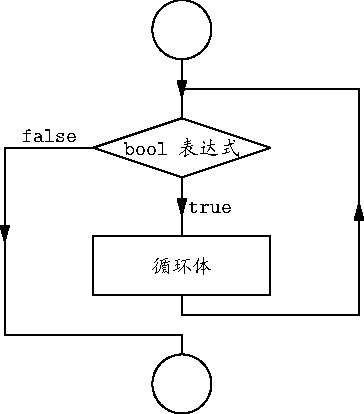
\includegraphics{graph/while.pdf}
    \caption{while工作流程}
  \label{fig:while_workflow}
\end{figure}

\lstinputlisting[aboveskip=5pt,belowskip=5pt,language=bash]{src/shell03.sh}

我们可以将while循环和专用命令“:”结合使用来定义。由于循环固有的一个特性,
当条件永远不被满足时,就会产生一个无限循环。定义一个while无限循环可以使
用如下三种命令:

\begin{enumerate}
\item true命令 \- 不做任何事情,表示成功,总是返回退出状态码0
\item false命令 \- 不做任何事情,表示失败,总是返回退出状态码1
\item :命令 \- 无作用,此命令也不做任何事情,总是返回退出状态码0
\end{enumerate}

\section{操作字符串}

\section{函数}

当我们的脚本大到一定程度时,使用函数则可以简化脚本,使程序结构更为清晰。

\section{信号捕捉}

\begin{verbatim}
trap可以捕捉信号,根据捕捉到的信号,执行响应的操作。
语法:
trap 'action' SIGNAL
\end{verbatim}

\section{开机脚本启动顺序}

\section{一个实例}

\lstinputlisting[aboveskip=5pt,belowskip=5pt,language=bash]{src/shell04.sh}

下面是该脚本的输出结果:

\begin{lstlisting}[numbers=none,aboveskip=5pt,belowskip=5pt]
System Report for richard on Tue Sep 23 21:34:22 CST 2014

Hostname: richard NIS Domain: (none)
Processor: 
Running at 4585.16
4585.16
4585.16
4585.16 bogomips with 3072 KB
3072 KB
3072 KB
3072 KB cache

OS Type: Linux Kernel:3.13.0-35-generic
Kernel Compile #62-Ubuntu on
Uptime: .08 days
Memory: 6003456 kB Free:   : 100
Swap: 6180860 kB Free:   : 100

Load Avderage:0.63 0.69 0.61 
Process Count:  total 1 running sleeping 0 stopped 0 zombie
\end{lstlisting}

\part{数据库篇}
\chapter{MySQL数据库基本知识}

MySQL\index{MySQL}是一个关系型数据库管理系统,由瑞典MySQL AB公司开发,
目前属于Oracle公司。MySQL是一个命途多舛的产品,2008年2月26日被Sun完全收
购,2009年4月20日Oracle并购了Sun公司。业界一片哗然,一时众说纷纭,褒贬
不一。在此过程中衍生出了两个版本的数据库,一个是Percona
Server及MariaDB,这些版本的衍生,是考虑到Oracle将其闭源的潜在可能。

关系型数据库将数据保存在不同的表中,而不是将所有数据放在一个大仓库内,
这样就增加了速度并提高了灵活性。MySQL所使用的SQL语言是用于访问数据库的
最常用标准化语言。MySQL软件采用了双授权策略,它分为
社区版和商业版,由于其体积小、速度快、总体拥有成本低,尤其是开放源码这
一特点,一般中小型网站的开发都选择MySQL作为其网站的数据库。由于其社区版的性
能卓越,搭配PHP和Apache可组成良好的开发环境。

\section{存储设备配置}

\subsection{构建文件系统}

使用xfs文件系统来提供MySQL数据的存储。使用xfs的话,需要添加管理配置工具
包,如下:

\begin{verbatim}
A0305010:~ # zypper -y install xfsdump xfsprogs   
A0305010:~ # modprobe -v xfs 
insmod /lib/modules/3.0.13-0.27-default/kernel/fs/xfs/xfs.ko
\end{verbatim}

使用mkfs.xfs创建文件系统如下:

\begin{verbatim}
A0305010:~ # fdisk /dev/sdb
Command (m for help): n
Command action
   e   extended
   p   primary partition (1-4)
p
Partition number (1-4, default 1): 
Using default value 1
First sector (2048-121634815, default 2048): 
Using default value 2048
Last sector, +sectors or +size{K,M,G} (2048-121634815, default 121634815): 
Using default value 121634815

Command (m for help): w
The partition table has been altered!

Calling ioctl() to re-read partition table.
Syncing disks.
A0305010:~ # partprobe /dev/sdb
A0305010:~ # mkfs.xfs -f -i size=512,attr=2 -l lazy-count=1 \
> -d su=64k,sw=10 -L /data1 /dev/sdb1
\end{verbatim}

注:这里的sdb是我们使用的一个样例。不同SSD厂商的设备在系统里被识别的标
识不一定是/dev/sdb,根据实际情况选择合适的标示符(如,Fusion-io的设备在
本次测试中被识别为/dev/fioa;LSI的设备在本次测试中被识别
为/dev/sdb;Intel的设备在本次测试中被识别为/dev/nvme0n1;宝存的设备在本
次测试中被识别为/def/dfa)。

\subsection{挂载文件系统}

\begin{verbatim}
A0305010:~ # mkdir /data1
A0305010:~ # cd /data1
A0305010:~ # mkdir mysqldata1 mysqldata2 mysqldata3 mysqldata4
A0305010:~ # mount -t xfs -o defaults,rw,noatime,nodiratime,\
> noikeep,nobarrier,allocsize=8M,attr2,largeio,\
> inode64,swalloc /dev/sdb1  /data1
\end{verbatim}

在/etc/fstab中添加自动挂载参数如下:
\begin{verbatim}
/dev/sdb1  /data1 xfs defaults,rw,noatime,nodiratime,noikeep,nobarrier,allocsize=8M,attr2,largeio,inode64,swalloc  0  0
A0305010:~ # mount -a
\end{verbatim}

\section{安装MySQL}
\subsection{创建MySQL用户}

我们需要添加专门的MySQL用户,并设置它的uid及gid为601。

\small{
\begin{verbatim}
[root@iLiuc ~]# groupadd -g 601 mysql
[root@iLiuc ~]# useradd -c "mysql software owner" -g mysql \
> -u 601 -m -d /home/mysql mysql
\end{verbatim}
}
\normalsize

\subsection{安装MySQL}

采用二进制方案安装,步骤如下:
\begin{enumerate}[itemsep=0pt,parsep=0pt]
\item 首先获取与生产环境数据库相同的二进制安装文件
\begin{verbatim}
A0305010:~ # mkdir /home/mysql/program
A0305010:~ # cd /home/mysql/program
A0305010:~ # ls
p16901968_55_Linux-x86-64.zip
\end{verbatim}
\item 解压
\begin{verbatim}
A0305010:~ # unzip p16901968_55_Linux-x86-64.zip
A0305010:~ # ls
README.txt
keepalived-1.2.7-8.1.x86_64.rpm
mysql-advanced-5.5.32-linux2.6-x86_64.tar.gz
mysql-advanced-5.5.32-linux2.6-x86_64.tar.gz.asc
mysql-advanced-5.5.32-linux2.6-x86_64.tar.gz.md5
p16901968_55_Linux-x86-64.zip
A0305010:~ # tar -xf mysql-advanced-5.5.32-linux2.6-x86_64.tar.gz
\end{verbatim}
\item 创建数据目录
\begin{verbatim}
A0305010:~ # mkdir /home/mysql/data
A0305010:~ # cd /home/mysql/data
A0305010:~ # mkdir conf innodb_log innodb_ts log mydata \
> relaylog slowlog sock tmpdir undo binlog
\end{verbatim}
\item 初始化MySQL元数据
\begin{verbatim}
A0305010:~ # cd /home/mysql/program/mysql-advanced-5.5.32-linux2.6-x86_64
A0305010:~ # ./scripts/mysql_install_db \
> --defaults-file=/home/mysql/conf/my1.cnf \
> --user=mysql \
> --skip-name-resolve
\end{verbatim}
\item 链接到/usr/local/mysql
\begin{verbatim}
A0305010:~ # ln -s /home/mysql/program/mysql-advanced-5.5.32-linux2.6-x86_64 \
> /usr/local/mysql
A0305010:~ # ln -s /data1/mysqldata1 /home/mysql/data/mysqldata1
A0305010:~ # ln -s /data1/mysqldata2 /home/mysql/data/mysqldata2
A0305010:~ # ln -s /data1/mysqldata3 /home/mysql/data/mysqldata3
A0305010:~ # ln -s /data1/mysqldata4 /home/mysql/data/mysqldata4
\end{verbatim}
\end{enumerate}

\small{
\begin{verbatim}
[root@iLiuc ~]# groupadd -g 601 mysql
[root@iLiuc ~]# useradd -c "mysql software owner" -g mysql \
> -u 601 -m -d /home/mysql mysql
\end{verbatim}
}
\normalsize

\section{操作系统配置}
\subsection{进程文件数配置}

由于MySQL采用多线程形式,每个进程打开的文件数要求比较高。所以我们需要增
加ulimit进程文件数的限制。在/etc/rc.local中添加:

\begin{verbatim}
A0305010:~ # /etc/init.d/sshd stop
A0305010:~ # ulimit -HSn 65535
\end{verbatim}

把上述配置写到配置文件/etc/security/limits.conf,找到“\# End of file”,
在其上添加3行

\begin{verbatim}
A0305010:~ # vi /etc/security/limits.conf
* hard memlock unlimited
* soft memlock unlimited
*		-	nofile		65535
A0305010:~ # /etc/init.d/sshd start
\end{verbatim}

\subsection{sysctl配置}

修改sysctl,添加swapness并设置TIME\_WAIT的相关参数。避免内存被交换并且减
少TIME\_WAIT状态时间。

\begin{verbatim}
A0305010:~ # echo "vm.swappiness = 0" >>/etc/sysctl.conf
A0305010:~ # echo "net.ipv4.tcp_tw_reuse=1" >>/etc/sysctl.conf
A0305010:~ # echo "net.ipv4.tcp_tw_recycle=1" >>/etc/sysctl.conf
A0305010:~ # echo "net.ipv4.tcp_fin_timeout = 30" >>/etc/sysctl.conf
A0305010:~ # sysctl -p
\end{verbatim}

\subsection{cgroup配置}

我们只对cpu和内存做限制,所以只需要挂载两个子系统。另外,我们在本服务器
上计划启动4个实例,这四个实例分别属于四个组,mysql\_g1, mysql\_g2,
mysql\_g3, mysql\_g4。目前我们限制它们都在4个超线程并且每个实例的内存不
超过24G。如下:

\begin{verbatim}
A0305010:~ # zypper install -y libcgroup1
A0305010:~ # cat /etc/cgconfig.conf
mount {
    cpuset  = /cgroup/cpuset;
    memory  = /cgroup/memory;
}
group mysql_g1 {
    cpuset {
        cpuset.cpus = 17-20;
        cpuset.mems = 0;
    }
    memory {
        memory.limit_in_bytes=25769803776;
        memory.swappiness=0;
    }
}
group mysql_g2 {
    cpuset {
        cpuset.cpus = 12-16;
        cpuset.mems = 0;
    }
    memory {
        memory.limit_in_bytes=25769803776;
        memory.swappiness=0;
    }
}
group mysql_g3 {
    cpuset {
        cpuset.cpus = 5-8;
        cpuset.mems = 0;
    }
    memory {
        memory.limit_in_bytes=25769803776;
        memory.swappiness=0;
        }
}
group mysql_g4 {
    cpuset {
        cpuset.cpus = 1-4;
        cpuset.mems = 0;
    }
    memory {
        memory.limit_in_bytes=25769803776;
        memory.swappiness=0;
    }
}

A0305010:~ # /etc/init.d/cgconfig start
\end{verbatim}

\subsection{cgrule配置}

我们设置使用mysqld\_safe1启动的命令为mysql\_g1组,这样就可以限制它的CPU和
内存使用。其他的四个实例同样进行设置如下:

\begin{verbatim}
A0305010:~ # cat /etc/cgrules.conf
*:/usr/local/mysql/bin/mysqld_safe1    *    mysql_g1
*:/usr/local/mysql/bin/mysqld_safe2    *    mysql_g2
*:/usr/local/mysql/bin/mysqld_safe3    *    mysql_g3
*:/usr/local/mysql/bin/mysqld_safe4    *    mysql_g4

A0305010:~ # /etc/init.d/cgred start
\end{verbatim}

\section{MySQL配置}
\subsection{程序文件和目录配置}
\subsection{多实例配置}

\begin{enumerate}[itemsep=0pt,parsep=0pt]
\item my.cnf文件配置

  我们在/home/mysql/conf下保存着my1.cnf,my2.cnf,my3.cnf,my4.cnf。针对
  每一个数据库实例都有一个对应的配置文件。各个配置文件中都保存的是每个实
  例独立的配置。通过“实例切换配置”来切换到各个不同的实例。

\item 实例切换配置

  我们在/home/mysql/bin下存放有四个文件my1,my2,my3,my4。用于切换到各
  个实例的配置环境中。并且我们在profile中添加了对应的别名:

\begin{verbatim}
alias my1=". /home/mysql/bin/my1"
alias my2=". /home/mysql/bin/my2"
alias my3=". /home/mysql/bin/my3"
alias my4=". /home/mysql/bin/my4"
\end{verbatim}

  如,my1文件内容如下:

\begin{verbatim}
#!/bin/sh
#****************************************************************#
# ScriptName: my1
#             switch to mysql instance 1 environment
# Author:
# Create Date: 2013-03-27
# Modify Author:
# Modify Date: 2013-03-27
# Function:
#***************************************************************#
#set -x

#### variable should change every instance
export INSTANCE_NO=1

#### variable should change every instance
export MYSQL_PORT=$(expr 3305 + $INSTANCE_NO)
export MYSQL_PROGRAM=/usr/local/mysql
export DATA_DIR=/home/mysql/data/mysqldata$INSTANCE_NO/
export MYSQL_CONF=/home/mysql/conf/my$INSTANCE_NO.cnf
export PS1="\n\e[1;37m[\e[m\e[1;36mMySQL$INSTANCE_NO\e[m \$(date \"+%Y-%m-%d %H:%M:%S\") \e[1;31m\u@\e[m\e[1;31m\h\e[m \e[4m\$(pwd)\e[m\e[1;37m]\e[m\e[1;36m\e[m\n\$"
alias stopmysql="$MYSQL_PROGRAM/bin/mysqladmin --defaults-file=$MYSQL_CONF -uroot -p111111 -hlocalhost -P$MYSQL_PORT shutdown"
alias my="$MYSQL_PROGRAM/bin/mysql --defaults-file=$MYSQL_CONF -uroot -p111111 -hlocalhost -P$MYSQL_PORT test --prompt='[$(whoami)@$(hostname):$(pwd) \\v_Instance$INSTANCE_NO \\u@\\h:\\d \\R:\\m:\\s] >'"

#### variable should not change every version
export PATH=$MYSQL_PROGRAM/bin/:$PATH
export LD_LIBRARY_PATH=$MYSQL_PROGRAM/lib/
export PROMPT_COMMAND='echo -ne "\033]0;${USER}@${HOSTNAME%%.*}"; echo -ne "\007"'

startmysql()
{
	cd $MYSQL_PROGRAM/
	$MYSQL_PROGRAM/bin/mysqld_safe$INSTANCE_NO --defaults-file=${MYSQL_CONF} & cd -
}

alias cdd="cd $DATA_DIR"
alias cdb="cd $MYSQL_PROGRAM"
alias cdm="cd /home/mysql/"
alias cdqm="cd $QGUARD_BASEDIR"
alias vi="vim"
alias vie="vim $DATA_DIR/log/error.log"
alias cate="cat $DATA_DIR/log/error.log"
alias psm="ps -ef|grep $MYSQL_PROGRAM/bin/mysqld |grep -v grep"
alias ll='ls -l -G'
alias rm='rm -i'
alias cp='cp -i'
alias mv='mv -i'
\end{verbatim}

\end{enumerate}

直接输入命令my1就可以切换到mysql实例1的环境下。此时可以直接输入my1命令
登录第一个实例的mysql环境,输入stopmysql就可以停掉MySQL数据库,输
入startmysql就可以启动MySQL数据库。

另外,还做了一些简单方便的命令,以便管理:

\begin{quote}
  cdd用于切换到实例的数据目录
  cdm用于切换到MySQL根目录
  cdb用于切换到MySQL的程序文件目录
  psm用于输出MySQL数据库的进程和cgroup信息等
\end{quote}

\section{数据库日常管理}
\subsection{实例切换}
\subsection{MySQL启动}
\subsection{MySQL关闭}

\section{如何进入MySQL数据库}

进入MySQL数据库很简单,首先确保mysqld进程已经启动。如果没有启动,请参照
前面的命令启动之。只需要在命令行输入命令mysql回车即可,因为我们的IPTV系
统里的mysql的root账户是没有密码的。

\small{
\begin{verbatim}
[root@iLiuc ~]# mysql
mysql> show databases;      <- 查看我们有哪些库
+-------------------------+
| Database                |
+-------------------------+
| information_schema      | 
| clear_360fy             | <- 稍后我们将导出这个库 
| clear_iptv2x            | 
| clear_iptv_Skyworth     | 
| clear_qingpu_school     | 
| clear_vod_mingzhu       | 
| clear_vod_new           | 
| clear_vod_yiyuan        | 
| clear_xianhuashan       | 
| cleardb_str             | 
| happyview               | 
+-------------------------+

mysql> use clear_360fy;     <- 选择要使用的库
Database changed            <- 提示数据库已改变

mysql> show tables;         <- 查看clear_360fy库中有哪些表
+--------------------------+
| Tables_in_clear_360fy    |
+--------------------------+
| config                   | 
| directory                | 
| drinks_info_t            | 
| favorites                | 
| hotel_category           | 
| hotel_info               | 
| language                 | 
| livechannel              | 
| log                      | 
  ...         
| massage                  | 
| program                  | 
| user_group_matrix        | 
| users                    | 
| weather                  | 
| wel_message              | 
+--------------------------+
mysql> exit                 <- 退出数据库
[root@iLiuc ~]# 
\end{verbatim}
}
\normalsize

\section{如何建库建表}

当我们的数据很少时,把这些信息可以手工的记录在纸片上或其他介质上,管理
起来也是很方便的。现如今是信息的时代,我们总不能把数据还是记录在纸上或
龟壳上吧,管理起来非把人给累死。把数据存在易于管理的数据库系统中是明智
之举。

\section{简单sql语句的使用}

有了上面的介绍是不是想动手操练一番。首先确保你的系统中应该安装有mysql数
据软件;其次,要确保mysqld服务已经在运行;最后,要有数据库的用户名及密
码。这里我们使用Clear的用户名及密码为123456为演示环境。

\subsection{create语句的使用}

create可以创建库和表,首先我们以一个具体的例子来演示该命令如何使用。接
下来我们要创建这样一个库,库名为cc(clear company),表的名字为hr(human
resource)

\begin{table}[h]
  \centering
  \begin{tabular}{lrlr}
    \toprule
    id   & name    & deptname       & salary \\
    \midrule
    1    & james   & development    & 1000 \\
    2    & wade    & engineer       & 800 \\
    3    & bosh    & finance        & 600 \\
    4    & richard & sale           & 600 \\
    5    & laven   & it             & 1010 \\
    \bottomrule
  \end{tabular}
\end{table}

\small{
\begin{verbatim}
[root@iLiuc ~]# mysql
mysql> create database if not exists cc;

mysql> use cc;
mysql> create table hr (
       id int not null primary key,
       name char(10) not null,
       deptname char(15) not null,
       salary float(5,2) not null);

mysql> desc hr;
+----------+------------+------+-----+---------+-------+
| Field    | Type       | Null | Key | Default | Extra |
+----------+------------+------+-----+---------+-------+
| id       | int(11)    | NO   | PRI | NULL    |       | 
| name     | char(10)   | NO   |     | NULL    |       | 
| deptname | char(15)   | NO   |     | NULL    |       | 
| salary   | float(5,2) | NO   |     | NULL    |       | 
+----------+------------+------+-----+---------+-------+
\end{verbatim}
}
\normalsize

上面的具体含义,我就不详细讲解了,自己去Google上Baidu一下吧。上面只是把
一个框架给搭建了起来,里面并没有任何数据,我们可以查看一下:

\begin{verbatim}
mysql> select * from hr;
Empty set (0.02 sec) <- 你将会看到这样的提示
\end{verbatim}

\subsection{insert语句的使用}

insert就是往表里面添加数据的,废话不多说,直接看例子:

\small{
\begin{verbatim}
mysql> insert into hr values
       (1, "james", "development", 1000),
       (2, "wade", "engineer", 800),
       (3, "bosh", "finance", 600),
       (4, "richard", "sale", 600),
       (5, "laven", "it", 1010);

mysql> select * from hr;
+----+---------+-------------+--------+
| id | name    | deptname    | salary |
+----+---------+-------------+--------+
|  1 | james   | development | 999.99 | 
|  2 | wade    | engineer    | 800.00 | 
|  3 | bosh    | finance     | 600.00 | 
|  4 | richard | sale        | 600.00 | 
|  5 | laven   | it          | 999.99 | 
+----+---------+-------------+--------+
\end{verbatim}
}
\normalsize

\subsection{select语句的使用}

select应该是数据库中使用最多的命令了,接下来赶紧介绍如何写select语句。

\small{
\begin{verbatim}
[root@iLiuc ~]# mysql -uroot -p123456
mysql> use clear_360fy;
mysql> select * from maincontrol;
...
\end{verbatim}
}
\normalsize

*是通配符,表示所有。上面的语句意思是查看maincontrol表的所有字段。
如果只查看某个字段或某几个字段,该怎么办呢?各字段之间用逗号分开即
可。每个表有哪些字段呢?使用desc查看即可。下面看演示:

\small{
\begin{verbatim}
mysql> desc maincontrol;

mysql> select * from hr;
+----+---------+-------------+--------+
| id | name    | deptname    | salary |
+----+---------+-------------+--------+
|  1 | james   | development | 999.99 | 
|  2 | wade    | engineer    | 800.00 | 
|  3 | bosh    | finance     | 600.00 | 
|  4 | richard | sale        | 600.00 | 
|  5 | laven   | it          | 999.99 | 
+----+---------+-------------+--------+
\end{verbatim}
}
\normalsize

\subsection{update语句的使用}

当有更新的操作时,update命令就派上用场了。当我们忘记信息发布或IPTV后台
的密码时,也是可用用到update语句的,接下来我们看看如何使用。

\small{
\begin{verbatim}
[root@iLiuc ~]# mysql
mysql> use clear_360fy;
mysql> show tables; <- 找到users
mysql> desc users; <- 查看users有哪些字段
+-------------------+
| Field             | 其他列我省略了
+-------------------+
| ID                |
| NAME              | <- 这是用户名
| PASSWORD          | <- 这是密码
| EMAIL             |
| TYPE              |
| 此处省略若干行...
| IDCARD            |
| ADDRESS           |
| TEL               |
+-------------------+

mysql> select name, password from users;
+-------------+----------------------------------+
| name        | password                         |
+-------------+----------------------------------+
| master      | eb0a191797624dd3a48fa681d3061212 | 
| NULL        | aaabf0d39951f3e6c3e8a7911df524c2 | 
| NULL        | 4124bc0a9335c27f086f24ba207a4912 | 
| newmanager  | 81dc9bdb52d04dc20036dbd8313ed055 | 
| firstmanger | 202cb962ac59075b964b07152d234b70 | 
| 123         | 202cb962ac59075b964b07152d234b70 | 
+-------------+----------------------------------+
\end{verbatim}
}
\normalsize

这时,我们看到了后台用户及其密码。密码是使用md5方式加密的,不安全。我们
可以在数据库里查看某个字符串的md5值,如:

\small{
\begin{verbatim}
mysql> select md5("123456");
+----------------------------------+
| md5("123456")                    |
+----------------------------------+
| e10adc3949ba59abbe56e057f20f883e | 
+----------------------------------+
\end{verbatim}
}
\normalsize

发现没有,123456的md5值跟上面master用户密码的md5值一样,那说明
maser用户的密码为123456。即使我们不知道master用户的密码,我们
照样可以在数据库里更新它的密码。这里我们把它的密码改为“654321”,
看操作:

\small{
\begin{verbatim}
mysql> select md5("654321");
+----------------------------------+
| md5("654321")                    |
+----------------------------------+
| c33367701511b4f6020ec61ded352059 | 
+----------------------------------+
\end{verbatim}
}
\normalsize

用鼠标左键选择“c33367701511b4f6020ec61ded352059”,别把双引号也给选上了。
之后按下鼠标中键即可实现粘贴功能

\small{
\begin{verbatim}
mysql> update users set password="c33367701511b4f6020ec61ded352059" 
     > where name="master";
\end{verbatim}
}
\normalsize

或者一步到位:

\small{
\begin{verbatim}
mysql> update users set password=(select md5("654321")) where name="master";
\end{verbatim}
}
\normalsize

再次查询,验证是不是已经改变,这时可以使用新的密码登陆后台了。

\small{
\begin{verbatim}
mysql> select name, password from users where name="master";
+-------------+----------------------------------+
| name        | password                         |
+-------------+----------------------------------+
| master      | c33367701511b4f6020ec61ded352059 | 
+-------------+----------------------------------+
\end{verbatim}
}
\normalsize

\section{数据库文件的备份}

做完一个项目后的第一件事,就是做好现场的备份,包括前台、后台及数据库。
首先,这是一个很好的习惯。如果不这样,万一出现问题,又要重新部署,岂不
是x都碎了。

\subsection{数据库文件的导出}
\label{sec:exportData}

数据库文件的导出,我们这里使用mysqldump命令。别的不多说,直接介绍该命令
如何使用

\begin{verbatim}
[root@iLiuc ~]# mysqldump -u root -p password db_name > db_name.sql
\end{verbatim}

上面这是标准的数据库备份命令,root为数据的用户名,password为root用户的
密码,需要导出的数据库名字为db\_name,然后把数据保存到当前目录下
的db\_name.sql文件。在我们的IPTV系统里,mysql的root账户是没有密码的,如
果我们要备份clear\_360fy的库文件,则输入一下命令即可:

\small{
\begin{verbatim}
[root@iLiuc ~]# mysqldump clear_360fy > /home/clear_360fy.sql
这条命令意思是把clear_360fy的库dump到/home目录下的clear_360fy.sql文件
\end{verbatim}
}
\normalsize

\subsection{数据库文件的导入}
\label{sec:importData}

数据库文件导入的前提是准备要导入的sql文件,这里我们准备好
clear\_360fy.sql文件,然后创建相应的库,再然后把sql文件导入到刚创建的库
中,这里只介绍一种方法,仅供参考。

\small{
\begin{verbatim}
[root@iLiuc ~]# mysqladmin create clear_360fy 
[root@iLiuc ~]# mysql clear_360fy < /home/clear_360fy.sql
\end{verbatim}
}
\normalsize

这条命令意思是先创建clear\_360fy库,然后把/home目录下的clear\_360fy.sql
文件导入到该库中

\section{常用命令总结}

\begin{enumerate}[itemsep=0pt,parsep=0pt]
\item 刷新
\begin{verbatim}
flush privileges;
\end{verbatim}
\item 显示所有数据库
\begin{verbatim}
show databases;
\end{verbatim}
\item 打开数据库
\begin{verbatim}
use dbname;
\end{verbatim}
\item 显示当前数据中所有的表
\begin{verbatim}
show tables;
\end{verbatim}
\item 查看表结构
\begin{verbatim}
desc tables;
\end{verbatim}
\item 删除数据库
\begin{verbatim}
drop database dbname;
\end{verbatim}
\item 删除表
\begin{verbatim}
drop table tbname;
\end{verbatim}
\item 创建数据库
\begin{verbatim}
create database dbname;
\end{verbatim}
\item 查询
\item 查看用户权限
\end{enumerate}

\small{
\begin{verbatim}
# 查询
select 列名称 from 表名称;    

# 查看用户权限
show grants for repl;         

# 查看mysql进程
show processlist;             

# 查看所有用户
select user();                

# 查看主从状态
show slave status\G;          

# 查看所有参数变量
show variables; 

# 查看表的引擎状态
show table status             

# 表存在就删除
drop table if exists user                       

# 表不存在就创建
create table if not exists user                 

# 查询用户权限 先use mysql
select host, user, password from user;          

# 创建表
create table ka(ka_id varchar(6),qianshu int);  

# 查看系统的字符集和排序方式的设定
show variables like 'character_set_%';          

# 查看超时(wait_timeout)
show variables like '%timeout%';                

# 删除空用户
delete from user where user='';                 

# 删除用户
delete from user where user='sss' and host='localhost' ;    

# 改变现有的表使用的存储引擎
alter table mytable engine = MyISAM ;                       

# 查询表引擎
show table status from  库名  where Name='表名';            

# 创建表指定存储引擎的类型(MyISAM或INNODB)
CREATE TABLE innodb (id int, title char(20)) ENGINE = INNODB                     

# 创建主从复制用户
grant replication slave on *.* to '用户'@'%' identified by '密码';               

# 添加索引
ALTER TABLE player ADD INDEX weekcredit_faction_index (weekcredit, faction);     

# 插入字段
alter table name add column accountid(列名)  int(11) NOT NULL(字段不为空);       

# 更新数据
update host set monitor_state='Y',hostname='username' where ip='192.168.1.1';     

# 清除二进制文件
purge binary logs to 'mysql-bin.000051';
\end{verbatim}
}
\normalsize

\subsection{忘记MySQL密码}
\label{sec:ForgotMysqlPass}

如果MySQL正在运行,首先停掉服务,然后终止进程;在安全模式下进入mysql数
据库去修改密码,最后重启mysqld服务。具体操作为:

\begin{verbatim}
# service mysqld stop
# killall -TERM mysqld
# mysqld_safe --skip-grant-tables &
# mysql
mysql> use mysql;
mysql> update user set password('new_pass') where user="root";
mysql> exit
# service mysqld restart
\end{verbatim}

\chapter{MySQL复制}

主服务器/从服务器设置增加了健壮性。主服务器出现问题时,可以切换到从服务
器。

通过在主服务器和从服务器之间切分处理客户查询的负荷,可以得到更好的客户
响应时间。SELECT查询可以发送到从服务器以降低主服务器的查询处理负荷。但
修改数据的语句仍然应发送到主服务器,以便主服务器和从服务器保持同步。

MySQL提供了数据库的同步功能,这对实现数据库的冗灾、备份、恢复、负载均衡
等都是有极大帮助的。

\section{复制如何工作}

MySQL复制数据,总的来说,有三个步骤:

\begin{enumerate}[itemsep=0pt,parsep=0pt]
\item 在主库上把数据更改记录到二进制日志(Binary Log)中(这些记录被称为
  二进制日志事件)。
\item 备库将主库上的日志复制到自己的中继日志(Relay Log)中。
\item 备库读取中继日志中的事件,将其重放到备库数据之上。
\end{enumerate}

复制如何工作:
\begin{figure}[!h]
\centering
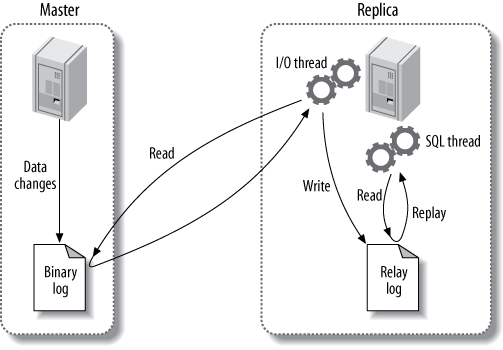
\includegraphics{img/mysql_replication_works}
\caption{MySQL复制的工作原理}
\label{fig:mysqlReplicationWorks}
\end{figure}

第一步是在主库上记录二进制日志。在每次准备提交事务完成数据更新前,主库
将数据更新的事件记录到二进制日志中。MySQL会按事务提交的顺序而非每条语句
的执行顺序来记录二进制日志。在记录二进制日志后,主库会告诉存储引擎可以
提交事务了。

下一步,备库将主库的二进制日志复制到其本地的中继日志中。首先,备库会启
动一个工作线程,称为I/O线程,I/O线程跟主库建立一个普通的客户端连接,然
后在主库上启动一个特殊的二进制转储(binlog dump)线程(该线程没有对应
的SQL命令),这个二进制转储线程会读取主库上二进制日志中的事件。它不会对
事件进行轮询。如果该线程追赶上了主库,它将进入睡眠状态,直到主库发送信
号量通知其有新的事件产生时才会被唤醒,备库I/O线程会将接收到的事件记录到
中继日志中。

备库的SQL线程执行最后一步,该线程从中继日志中读取事件并在备库执行,从而
实现备库数据的更新。当SQL线程追赶上I/O线程时,中继日志通常已经在系统缓
存中了,所以中继日志的开销很低。SQL线程执行的事件也可以通过配置选项来决
定是否写入其自己的二进制日志中。

这种复制架构实现了获取事件的重放事件的解耦,允许这两个过程异步进行。也
就是说I/O线程能够独立于SQL线程之外工作。但这种架构也限制了复制的过程,
其中最重要的一点是在主库上并发运行的查询在备库上只能串化执行,因为只有
一个SQL线程来重放中继日志的事件。

\section{MySQL复制原理}

MySQL支持单向、双向复制、异步复制,复制过程中一个服务器充当主服务器,而
一个或多个其他服务器充当从服务器。主服务器将更新写入一个二进制日志文件
中,并创建一个索引文件以跟踪日志循环。这些日志文件可以将记录发送到从服
务器以让从服务器保持与主服务器的数据一致。当一个从服务器连接主服务器时,
日志文件会通知主服务器,从服务器在上次成功更新的位置处开始进入更新操作。
更新完成后从服务器开始进入等待状态,等待主服务器后续的更新。

\section{MySQL同步细节}

MySQL同步功能由3个线程(Master上1个binlog dump,Slave上2个,分别是SQL进
程和IO进程)来实现。执行“START SLAVE”语句后,Slave就创建

\section{MySQL半同步配置}

\begin{enumerate}[itemsep=0pt,parsep=0pt]
\item 检查是否支持动态加载

登录MySQL并查询have\_dynamic\_loading变量
\begin{verbatim}
mysql_master> show variables like  'have_dynamic_loading';
mysql_slave> show variables like  'have_dynamic_loading';
+----------------------+-------+
| Variable_name        | Value |
+----------------------+-------+
| have_dynamic_loading | YES   |
+----------------------+-------+
1 row in set (0.00 sec)
\end{verbatim}
\item 确认lib/plugin目录下有半同步插件so

  确认主库MySQL程序目录下有lib/plugin/semisync\_master.so文件,确认备
  库MySQL程序目录下有lib/plugin/semisync\_slave.so文件

\begin{verbatim}
ls /usr/local/mysql/lib/plugin
adt_null.so           auth.so               auth_test_plugin.so    
daemon_example.ini    libdaemon_example.so  qa_auth_client.so     
qa_auth_server.so     semisync_slave.so     audit_log.so          
auth_socket.so        authentication_pam.so debug               
mypluglib.so          qa_auth_interface.so  semisync_master.so
thread_pool.so
\end{verbatim}

\item 主库动态加载半同步插件

登录MySQL并加载主库半同步插件,并设置主库半同步有效
\begin{verbatim}
mysql_master> INSTALL PLUGIN rpl_semi_sync_master SONAME 'semisync_master.so';
mysql_master> set global rpl_semi_sync_master_enabled=on
mysql_master> set global rpl_semi_sync_master_timeout=1000
\end{verbatim}
\item 备库动态加载半同步插件
\begin{verbatim}
mysql_slave> INSTALL PLUGIN rpl_semi_sync_slave SONAME 'semisync_slave.so';
mysql_slave> set global rpl_semi_sync_slave_enabled=on; 
\end{verbatim}
\item 主库MySQL配置文件修改

为了保证主库MySQL再次重启服务器后自动打开半同步,需要增加主库MySQL配置如下:
\begin{verbatim}
rpl_semi_sync_master_enabled=1
rpl_semi_sync_master_timeout=1000
\end{verbatim}
\item 备库MySQL配置文件修改

为了保证备库MySQL再次重启服务器后自动打开半同步,需要增加备库MySQL配置如下:
\begin{verbatim}
rpl_semi_sync_slave_enabled=1
\end{verbatim}
\item 备库MySQL重新连接

为了保证主备库是以半同步方式复制的,建议备库上重启复制:
\begin{verbatim}
root@slave >stop slave ; start slave;
\end{verbatim}
\end{enumerate}

\chapter{MySQL+KeepAlived}

\section{KeepAlived介绍}
Keepalived is a routing software written in C. The main goal of this
project is to provide simple and robust facilities for loadbalancing
and high-availability to Linux system and Linux based
infrastructures. Loadbalancing framework relies on well-known and
widely used Linux Virtual Server (IPVS) kernel module providing Layer4
loadbalancing. Keepalived implements a set of checkers to dynamically
and adaptively maintain and manage loadbalanced server pool according
their health. On the other hand high-availability is achieved by VRRP
protocol. VRRP is a fundamental brick for router failover. In
addition, Keepalived implements a set of hooks to the VRRP finite
state machine providing low-level and high-speed protocol
interactions. Keepalived frameworks can be used independently or all
together to provide resilient infrastructures.

使用MySQL双master+keepalived是一种非常好的解决方案,在MySQL-HA环境
中,MySQL互为主从关系,这样就保证了两台MySQL数据的一致性,然后
用KeepAlived实现虚拟IP,通过KeepAlived自带的服务监控功能来实现MySQL故障
时自动切换。

\begin{verbatim}
环境:
mysql_01: 
hostname A0304010 172.16.25.39

mysql_02:
hostname A0305010 172.16.25.40

各个主机授权:
mysql_01> grant replication slave on *.* to 'repl01'@'%' identified by 'replpass';
mysql_01> flush privileges;

mysql_02> grant replication slave on *.* to 'repl02'@'%' identified by 'replpass';
mysql_02> flush privileges;

查看各主机的日志文件及日志位置:
mysql_01> show master status\G
*************************** 1. row ***************************
            File: mysql-bin.000076
        Position: 346
    Binlog_Do_DB: 
Binlog_Ignore_DB: 
1 row in set (0.00 sec)

mysql_02> show master status\G
*************************** 1. row ***************************
            File: mysql-bin.000076
        Position: 346
    Binlog_Do_DB: 
Binlog_Ignore_DB: 
1 row in set (0.00 sec)

各主机change master to:
mysql_01> change master to
    -> master_host='172.16.25.40',
    -> master_user='repl02',
    -> master_password='replpass',
    -> master_port=3313,
    -> master_log_file='mysql-bin.000076',
    -> master_log_pos=346;
Query OK, 0 rows affected (0.35 sec)

mysql_01> start slave;
mysql_01> show slave status\G
*************************** 1. row ***************************
               Slave_IO_State: Waiting for master to send event
                  Master_Host: 172.16.25.40
                  Master_User: repl02
                  Master_Port: 3313
                Connect_Retry: 60
              Master_Log_File: mysql-bin.000076
          Read_Master_Log_Pos: 346
               Relay_Log_File: mysql-relay-bin.000002
                Relay_Log_Pos: 253
        Relay_Master_Log_File: mysql-bin.000076
             Slave_IO_Running: Yes
            Slave_SQL_Running: Yes
              Replicate_Do_DB: 
          Replicate_Ignore_DB: 
           Replicate_Do_Table: 
       Replicate_Ignore_Table: 
      Replicate_Wild_Do_Table: 
  Replicate_Wild_Ignore_Table: 
                   Last_Errno: 0
                   Last_Error: 
                 Skip_Counter: 0
          Exec_Master_Log_Pos: 346
              Relay_Log_Space: 409
              Until_Condition: None
               Until_Log_File: 
                Until_Log_Pos: 0
           Master_SSL_Allowed: No
           Master_SSL_CA_File: 
           Master_SSL_CA_Path: 
              Master_SSL_Cert: 
            Master_SSL_Cipher: 
               Master_SSL_Key: 
        Seconds_Behind_Master: 0
Master_SSL_Verify_Server_Cert: No
                Last_IO_Errno: 0
                Last_IO_Error: 
               Last_SQL_Errno: 0
               Last_SQL_Error: 
  Replicate_Ignore_Server_Ids: 
             Master_Server_Id: 4008
1 row in set (0.00 sec)

mysql_02> change master to 
master_host='172.16.25.39', 
master_useser='repl01', 
master_password='replpass', 
master_port=3313, 
master_log_file='mysql-bin.000076', 
master_log_pos=346;
Query OK, 0 rows affected (0.20 sec)

mysql_02> start slave;
mysql_02> show slave status\G
*************************** 1. row ***************************
               Slave_IO_State: Waiting for master to send event
                  Master_Host: 172.16.25.39
                  Master_User: repl01
                  Master_Port: 3313
                Connect_Retry: 60
              Master_Log_File: mysql-bin.000076
          Read_Master_Log_Pos: 346
               Relay_Log_File: mysql-relay-bin.000002
                Relay_Log_Pos: 253
        Relay_Master_Log_File: mysql-bin.000076
             Slave_IO_Running: Yes
            Slave_SQL_Running: Yes
              Replicate_Do_DB: 
          Replicate_Ignore_DB: 
           Replicate_Do_Table: 
       Replicate_Ignore_Table: 
      Replicate_Wild_Do_Table: 
  Replicate_Wild_Ignore_Table: 
                   Last_Errno: 0
                   Last_Error: 
                 Skip_Counter: 0
          Exec_Master_Log_Pos: 346
              Relay_Log_Space: 409
              Until_Condition: None
               Until_Log_File: 
                Until_Log_Pos: 0
           Master_SSL_Allowed: No
           Master_SSL_CA_File: 
           Master_SSL_CA_Path: 
              Master_SSL_Cert: 
            Master_SSL_Cipher: 
               Master_SSL_Key: 
        Seconds_Behind_Master: 0
Master_SSL_Verify_Server_Cert: No
                Last_IO_Errno: 0
                Last_IO_Error: 
               Last_SQL_Errno: 0
               Last_SQL_Error: 
  Replicate_Ignore_Server_Ids: 
             Master_Server_Id: 3908
1 row in set (0.00 sec)

\end{verbatim}
\section{测试同步}

\begin{verbatim}
mysql_01> show databases;
+--------------------+
| Database           |
+--------------------+
| information_schema |
| mysql              |
| performance_schema |
| sbtest             |
| test               |
+--------------------+
5 rows in set (0.00 sec)

mysql_02> show databases;
+--------------------+
| Database           |
+--------------------+
| information_schema |
| mysql              |
| performance_schema |
| sbtest             |
| test               |
+--------------------+
5 rows in set (0.00 sec)

mysql_01> create database doublec;
mysql_02> show databases;
+--------------------+
| Database           |
+--------------------+
| information_schema |
| liucc              |
| mysql              |
| performance_schema |
| sbtest             |
| test               |
+--------------------+
6 rows in set (0.00 sec)

mysql_02> drop database doublec;
mysql_01> show databases;
+--------------------+
| Database           |
+--------------------+
| information_schema |
| mysql              |
| performance_schema |
| sbtest             |
| test               |
+--------------------+
5 rows in set (0.00 sec)
\end{verbatim}

\section{安装配置KeepAlived}
\begin{verbatim}
安装配置keepalived:
A0304010:
rpm -qa |grep keepalived
keepalived-1.2.7-8.1

cat /etc/keepalived/keepalived.conf
! Configuration File for keepalived

global_defs {
   router_id LVS_DEVEL
}

vrrp_instance MySQL_Loadblancing {
    state BACKUP
    interface vlan0
    virtual_router_id 7
    priority 250
    advert_int 1
    nopreempt
    authentication {
        auth_type PASS
        auth_pass 1111
    }
    virtual_ipaddress {
        172.16.25.7
    }
}

virtual_server 172.16.25.7 3313 {
    delay_loop 6
    lb_algo wrr
    lb_kind DR
    protocol TCP
    persistence_timeout 50

    real_server 172.16.25.39 3313 {
        weight 3
        notify_down /home/mysql/bin/kill_keepalived.sh
        TCP_CHECK {
            connect_timeout 3
            nb_get_retry 3
            delay_before_retry 3
            connect_port 3306
        }
    }
}  

cat /home/mysql/bin/kill_keepalived.sh
#!/bin/bash
pkill keepalived


A0305010:
rpm -qa |grep keepalived
keepalived-1.2.7-8.1

cat /etc/keepalived/keepalived.conf
! Configuration File for keepalived

global_defs {
   router_id LVS_DEVEL
}

vrrp_instance MySQL_Loadblancing {
    state BACKUP
    interface vlan0
    virtual_router_id 7
    priority 200
    advert_int 1
    authentication {
        auth_type PASS
        auth_pass 1111
    }
    virtual_ipaddress {
        172.16.25.7
    }
}

virtual_server 172.16.25.7 3313 {
    delay_loop 6
    lb_algo wrr
    lb_kind DR
    protocol TCP
    persistence_timeout 50

    real_server 172.16.25.40 3313 {
        weight 3
        notify_down /home/mysql/bin/kill_keepalived.sh
        TCP_CHECK {
            connect_timeout 3
            nb_get_retry 3
            delay_before_retry 3
            connect_port 3313
        }
    }
}  

cat /home/mysql/bin/kill_keepalived.sh 
#!/bin/bash
pkill keepalived

\end{verbatim}

\section{启动KeepAlived}

\begin{verbatim}
启动keepalived服务,验证VIP:
A0304010:
/etc/init.d/keepalivd start
ip a
......
8: vlan0@bond0: <BROADCAST,MULTICAST,UP,LOWER_UP> mtu 1500 qdisc noqueue state UP 
    link/ether 6c:92:bf:0a:73:e3 brd ff:ff:ff:ff:ff:ff
    inet 172.16.25.39/24 brd 172.16.25.255 scope global vlan0
    inet 172.16.25.7/32 scope global vlan0
    inet6 fe80::6e92:bfff:fe0a:73e3/64 scope link 
       valid_lft forever preferred_lft forever
......

A0304010:
mysql_01> select host, user from mysql.user;
+-----------+--------+
| host      | user   |
+-----------+--------+
| %         | repl   |
| %         | repl01 |
| %         | sbtest |
| localhost | root   |
+-----------+--------+
4 rows in set (0.00 sec)


A0305010:
/etc/init.d/keepalived start
ip a
......
8: vlan0@bond0: <BROADCAST,MULTICAST,UP,LOWER_UP> mtu 1500 qdisc noqueue state UP 
    link/ether 6c:92:bf:0a:53:07 brd ff:ff:ff:ff:ff:ff
    inet 172.16.25.40/24 brd 172.16.25.255 scope global vlan0
    inet6 fe80::6e92:bfff:fe0a:5307/64 scope link 
       valid_lft forever preferred_lft forever
......

在其他机器上,测试VIP的连通性:
A0304006:
ping 172.16.25.7
PING 172.16.25.7 (172.16.25.7) 56(84) bytes of data.
64 bytes from 172.16.25.7: icmp_seq=1 ttl=64 time=0.174 ms
64 bytes from 172.16.25.7: icmp_seq=2 ttl=64 time=0.143 ms
64 bytes from 172.16.25.7: icmp_seq=3 ttl=64 time=0.151 ms
64 bytes from 172.16.25.7: icmp_seq=4 ttl=64 time=0.168 ms
64 bytes from 172.16.25.7: icmp_seq=5 ttl=64 time=0.174 ms
^C
--- 172.16.25.7 ping statistics ---
5 packets transmitted, 5 received, 0% packet loss, time 3998ms
rtt min/avg/max/mdev = 0.143/0.162/0.174/0.012 ms

在其他机器上登陆VIP,进行验证:
A0304002:~ # mysql -h172.16.25.39 -usbtest -P3313 -p
Enter password: 
Welcome to the MySQL monitor.  Commands end with ; or \g.
Your MySQL connection id is 217
Server version: 5.5.32-enterprise-commercial-advanced-log MySQL Enterprise Server - Advanced Edition (Commercial)

Type 'help;' or '\h' for help. Type '\c' to clear the current input statement.

mysql>mysql> use sbtest;
Database changed
mysql> show tables;
+------------------+
| Tables_in_sbtest |
+------------------+
| sbtest1          | 
| sbtest10         | 
| sbtest11         | 
| sbtest12         | 
| sbtest13         | 
| sbtest14         | 
| sbtest15         | 
| sbtest16         | 
| sbtest17         | 
| sbtest18         | 
| sbtest19         | 
| sbtest2          | 
| sbtest20         | 
| sbtest21         | 
| sbtest22         | 
| sbtest23         | 
| sbtest24         | 
| sbtest3          | 
| sbtest4          | 
| sbtest5          | 
| sbtest6          | 
| sbtest7          | 
| sbtest8          | 
| sbtest9          | 
+------------------+
24 rows in set (0.00 sec)


root@A0304010 /data1]
$netstat -antup |grep 3313
tcp        0      0 0.0.0.0:3313            0.0.0.0:*               LISTEN      10896/mysqld        
tcp        0      0 172.16.25.39:45087      172.16.25.40:3313       ESTABLISHED 10896/mysqld        
tcp        0      0 172.16.25.39:3313       172.16.25.40:42982      ESTABLISHED 10896/mysqld        
tcp        0      0 172.16.25.39:3313       172.16.25.32:32845      ESTABLISHED 10896/mysqld        


MySQL8 2014-12-26 12:20:14 root@A0305010 /data1]
$netstat -antup |grep 3313
tcp        0      0 0.0.0.0:3313            0.0.0.0:*               LISTEN      25423/mysqld        
tcp        0      0 172.16.25.40:3313       172.16.25.39:45087      ESTABLISHED 25423/mysqld        
tcp        0      0 172.16.25.40:42982      172.16.25.39:3313       ESTABLISHED 25423/mysqld   

停掉25.39的MySQL:     
[MySQL8 2014-12-26 12:48:32 root@A0304010 /data1]
$netstat -antup |grep 3313
tcp        0      0 172.16.25.39:45087      172.16.25.40:3313       FIN_WAIT2   -                   
tcp        0      0 172.16.25.39:3313       172.16.25.40:42982      TIME_WAIT   -                   
tcp        0      0 172.16.25.39:3313       172.16.25.32:32845      FIN_WAIT2   -     

              
/etc/init.d/keepalived status
Checking for Keepalived daemon                                   unused


故障切换:
172.16.25.36为客户端,连接VIP来进行查询,
首先,停掉25.39的MySQL服务,验证25.39上的keepalived是不是被停掉了。
ip a
......
8: vlan0@bond0: <BROADCAST,MULTICAST,UP,LOWER_UP> mtu 1500 qdisc noqueue state UP 
    link/ether 6c:92:bf:0a:73:e3 brd ff:ff:ff:ff:ff:ff
    inet 172.16.25.39/24 brd 172.16.25.255 scope global vlan0
    inet 172.16.25.7/32 scope global vlan0
    inet6 fe80::6e92:bfff:fe0a:73e3/64 scope link 
       valid_lft forever preferred_lft forever
......

然后,查看25.36客户端的连接情况。
A0304002:~ # mysql -h172.16.25.7 -usbtest -P3313 -p
Enter password: xxxxxx
Welcome to the MySQL monitor.  Commands end with ; or \g.
Your MySQL connection id is 83
Server version: 5.5.32-enterprise-commercial-advanced-log MySQL Enterprise Server - Advanced Edition (Commercial)

Type 'help;' or '\h' for help. Type '\c' to clear the current input statement.

mysql> show databases;
+--------------------+
| Database           |
+--------------------+
| information_schema | 
| sbtest             | 
| test               | 
+--------------------+
3 rows in set (0.00 sec)

mysql> use sbtest;
mysql> show tables;
+------------------+
| Tables_in_sbtest |
+------------------+
| sbtest1          | 
| sbtest10         | 
| sbtest11         | 
| sbtest12         | 
| sbtest13         | 
| sbtest14         | 
| sbtest15         | 
| sbtest16         | 
| sbtest17         | 
| sbtest18         | 
| sbtest19         | 
| sbtest2          | 
| sbtest20         | 
| sbtest21         | 
| sbtest22         | 
| sbtest23         | 
| sbtest24         | 
| sbtest3          | 
| sbtest4          | 
| sbtest5          | 
| sbtest6          | 
| sbtest7          | 
| sbtest8          | 
| sbtest9          | 
+------------------+
24 rows in set (0.00 sec)

mysql> show tables;
ERROR 1053 (08S01): Server shutdown in progress

mysql> show tables;
No connection. Trying to reconnect...
ERROR 2003 (HY000): Can't connect to MySQL server on '172.16.25.7' (113)
ERROR: 
Can't connect to the server

mysql> show tables;
ERROR 2013 (HY000): Lost connection to MySQL server during query
mysql> show tables;
ERROR 2006 (HY000): MySQL server has gone away
No connection. Trying to reconnect...
Connection id:    22
Current database: sbtest

+------------------+
| Tables_in_sbtest |
+------------------+
| sbtest1          | 
| sbtest10         | 
| sbtest11         | 
| sbtest12         | 
| sbtest13         | 
| sbtest14         | 
| sbtest15         | 
| sbtest16         | 
| sbtest17         | 
| sbtest18         | 
| sbtest19         | 
| sbtest2          | 
| sbtest20         | 
| sbtest21         | 
| sbtest22         | 
| sbtest23         | 
| sbtest24         | 
| sbtest3          | 
| sbtest4          | 
| sbtest5          | 
| sbtest6          | 
| sbtest7          | 
| sbtest8          | 
| sbtest9          | 
+------------------+
24 rows in set (0.02 sec)


最后,查看25.40的keepalived状态及连接情况。
ip a
......
8: vlan0@bond0: <BROADCAST,MULTICAST,UP,LOWER_UP> mtu 1500 qdisc noqueue state UP 
    link/ether 6c:92:bf:0a:53:07 brd ff:ff:ff:ff:ff:ff
    inet 172.16.25.40/24 brd 172.16.25.255 scope global vlan0
    inet 172.16.25.7/32 scope global vlan0
    inet6 fe80::6e92:bfff:fe0a:5307/64 scope link 
......


$netstat -antup |grep 3313
tcp        0      0 0.0.0.0:3313            0.0.0.0:*               LISTEN      28723/mysqld        
tcp        0      0 172.16.25.7:3313        172.16.25.32:43533      ESTABLISHED 28723/mysqld        

A0304010:
A0304010:~ # grep -v "^#" /home/mysql/conf/my8.cnf
[client]
loose_default-character-set = utf8
port=3313
socket=/home/mysql/data/mysqldata8/sock/mysql.sock
user=admin

[mysqld]
large-pages
read_only=off
memlock
default-storage-engine = INNODB
character-set-server=utf8
collation = utf8_bin

user=mysql
port=3313
socket=/home/mysql/data/mysqldata8/sock/mysql.sock
pid-file=/home/mysql/data/mysqldata8/sock/mysql.pid
datadir=/home/mysql/data/mysqldata8/mydata
tmpdir=/home/mysql/data/mysqldata8/tmpdir

skip-name-resolve
skip_external_locking

lower_case_table_names=1
event_scheduler=0
back_log=512
default-time-zone='+8:00'

max_connections = 3000
max_connect_errors=99999
max_allowed_packet = 64M
max_heap_table_size = 8M
max_length_for_sort_data = 16k

wait_timeout=172800
interactive_timeout=172800 

net_buffer_length = 8K
read_buffer_size = 2M
read_rnd_buffer_size = 2M
sort_buffer_size = 2M
join_buffer_size = 4M
binlog_cache_size = 2M
 
table_open_cache = 2048
table_definition_cache = 2048
thread_cache_size = 512
tmp_table_size = 8M

query_cache_size=0
query_cache_type=OFF


log-error=/home/mysql/data/mysqldata8/log/error.log
long_query_time = 1
slow_query_log
slow_query_log_file=/home/mysql/data/mysqldata8/slowlog/slow-query.log
log_warnings
log_slow_slave_statements


server-id=03908
log-bin=/home/mysql/data/mysqldata8/binlog/mysql-bin
binlog-format=ROW
max_binlog_size = 512M
expire_logs_days=15
sync_binlog=1
auto_increment_increment=2
auto_increment_offset=2

relay-log=/home/mysql/data/mysqldata8/relaylog/mysql-relay-bin
slave-skip-errors=1022,1032,1062
report-port=3313
log_bin_trust_function_creators=1
log_slave_updates=1


key_buffer_size = 8M
bulk_insert_buffer_size = 8M
myisam_sort_buffer_size = 64M
myisam_max_sort_file_size = 10G
myisam_repair_threads = 1
myisam_recover

innodb_data_home_dir = /home/mysql/data/mysqldata8/innodb_ts
innodb_data_file_path = ibdata1:2048M:autoextend
innodb_file_per_table
innodb_file_format = barracuda
innodb_file_format_max = barracuda
innodb_file_format_check = ON
innodb_strict_mode = 1
innodb_flush_method = O_DIRECT
innodb_autoinc_lock_mode=2

innodb_additional_mem_pool_size = 8M
innodb_buffer_pool_size = 1G
innodb_max_dirty_pages_pct = 75
innodb_adaptive_flushing = ON
innodb_change_buffering = inserts
innodb_old_blocks_time = 1000

innodb_log_group_home_dir = /home/mysql/data/mysqldata8/innodb_log
innodb_log_buffer_size = 64M
innodb_log_file_size = 2000M
innodb_log_files_in_group = 2
innodb_flush_log_at_trx_commit = 1
innodb_support_xa = ON

innodb_thread_concurrency = 32
innodb_lock_wait_timeout = 120
innodb_rollback_on_timeout = 1
transaction_isolation = READ-COMMITTED

innodb_read_io_threads = 4
innodb_write_io_threads = 12
innodb_io_capacity = 40000
innodb_use_native_aio = 1

innodb_purge_threads = 1

[mysqldump]
quick
max_allowed_packet = 2G
default-character-set = utf8

[mysql]
no-auto-rehash
show-warnings
prompt="5.1 \\u@\\h : \\d \\r:\\m:\\s> "
default-character-set = utf8

[myisamchk]
key_buffer = 512M
sort_buffer_size = 512M
read_buffer = 8M
write_buffer = 8M

[mysqlhotcopy]
interactive-timeout

[mysqld_safe]
user=mysql
open-files-limit = 8192

--------------------------------------------------------

A0305010:
$grep -v "^#" /home/mysql/conf/my8.cnf 
[client]
loose_default-character-set = utf8
port=3313
socket=/home/mysql/data/mysqldata8/sock/mysql.sock
user=admin

[mysqld]
large-pages
read_only=off
memlock
default-storage-engine = INNODB
character-set-server=utf8
collation = utf8_bin

user=mysql
port=3313
socket=/home/mysql/data/mysqldata8/sock/mysql.sock
pid-file=/home/mysql/data/mysqldata8/sock/mysql.pid
datadir=/home/mysql/data/mysqldata8/mydata
tmpdir=/home/mysql/data/mysqldata8/tmpdir

skip-name-resolve
skip_external_locking

lower_case_table_names=1
event_scheduler=0
back_log=512
default-time-zone='+8:00'

max_connections = 3000
max_connect_errors=99999
max_allowed_packet = 64M
max_heap_table_size = 8M
max_length_for_sort_data = 16k

wait_timeout=172800
interactive_timeout=172800 

net_buffer_length = 8K
read_buffer_size = 2M
read_rnd_buffer_size = 2M
sort_buffer_size = 2M
join_buffer_size = 4M
binlog_cache_size = 2M
 
table_open_cache = 2048
table_definition_cache = 2048
thread_cache_size = 512
tmp_table_size = 8M

query_cache_size=0
query_cache_type=OFF

log-error=/home/mysql/data/mysqldata8/log/error.log
long_query_time = 1
slow_query_log
slow_query_log_file=/home/mysql/data/mysqldata8/slowlog/slow-query.log
log_warnings
log_slow_slave_statements

server-id=04008
log-bin=/home/mysql/data/mysqldata8/binlog/mysql-bin
binlog-format=ROW
max_binlog_size = 512M
expire_logs_days=15
sync_binlog=1
auto_increment_increment=2
auto_increment_offset=2

relay-log=/home/mysql/data/mysqldata8/relaylog/mysql-relay-bin
slave-skip-errors=1022,1032,1062
report-port=3313
log_bin_trust_function_creators=1
log_slave_updates=1

key_buffer_size = 8M
bulk_insert_buffer_size = 8M
myisam_sort_buffer_size = 64M
myisam_max_sort_file_size = 10G
myisam_repair_threads = 1
myisam_recover

innodb_data_home_dir = /home/mysql/data/mysqldata8/innodb_ts
innodb_data_file_path = ibdata1:2048M:autoextend
innodb_file_per_table
innodb_file_format = barracuda
innodb_file_format_max = barracuda
innodb_file_format_check = ON
innodb_strict_mode = 1
innodb_flush_method = O_DIRECT
innodb_autoinc_lock_mode=2

innodb_additional_mem_pool_size = 8M
innodb_buffer_pool_size = 8M
innodb_max_dirty_pages_pct = 75
innodb_adaptive_flushing = ON
innodb_change_buffering = inserts
innodb_old_blocks_time = 1000

innodb_log_group_home_dir = /home/mysql/data/mysqldata8/innodb_log
innodb_log_buffer_size = 64M
innodb_log_file_size = 2000M
innodb_log_files_in_group = 2
innodb_flush_log_at_trx_commit = 1
innodb_support_xa = ON

innodb_thread_concurrency = 32
innodb_lock_wait_timeout = 120
innodb_rollback_on_timeout = 1
transaction_isolation = READ-COMMITTED

innodb_read_io_threads = 4
innodb_write_io_threads = 12
innodb_io_capacity = 40000
innodb_use_native_aio = 1

innodb_purge_threads = 1

[mysqldump]
quick
max_allowed_packet = 2G
default-character-set = utf8

[mysql]
no-auto-rehash
show-warnings
prompt="5.5 \\u@\\h : \\d \\r:\\m:\\s> "
default-character-set = utf8

[myisamchk]
key_buffer = 512M
sort_buffer_size = 512M
read_buffer = 8M
write_buffer = 8M

[mysqlhotcopy]
interactive-timeout

[mysqld_safe]
user=mysql
open-files-limit = 8192
\end{verbatim}

\chapter{MySQL+LVS}

\chapter{MHA}
\label{chap:mha}

本文介绍如何一步步搭建MHA高可用环境,

\section{实验环境说明}
\label{sec:MHAEnvSpecific}

使用的MySQL版本为5.5.32企业版,MHA版本为0.56版本,三台服务器。

\subsection{SSH无密码通信设置}
\label{sec:SSHSetup}

在所有机器上执行,设置SSH无密码通信:

\begin{verbatim}
# ssh-keygen -t rsa
# ssh-copy-id -i /root/.ssh/id_rsa.pub root@10.10.7.16
# ssh-copy-id -i /root/.ssh/id_rsa.pub root@10.10.7.17
# ssh-copy-id -i /root/.ssh/id_rsa.pub root@10.10.7.201
\end{verbatim}

\section{安装MySQL}
\label{InstallMySQL}

使用二进制的方式安装MySQL,

\section{安装及配置MHA}
\label{sec:InstallMHANode}

安装方式有两种,可以使用源代码编译安装或者使用RPM包进行安装。使用RPM包
安装简单些,本次安装使用RPM包方式进行安装。安装包可以到这
里https://code.google.com/p/mysql-master-ha/downloads/list下载。

\subsection{安装node节点}
\label{sec:InstallNode}

在所有机器上执行,安装mha的node节点,安装依赖包:

\begin{verbatim}
# yum install -y perl-DBD-MySQL
# rpm -ivh mha4mysql-node-0.56-0.el6.noarch.rpm
\end{verbatim}

\subsection{安装manager节点}
\label{sec:InstallManager}

在Slave机器上执行,安装mha的manager节点,

\begin{verbatim}
# yum install -y perl-Config-Tiny
# yum install -y perl-DBD-MySQL
# yum install -y perl-MIME-Lite
# yum install -y perl-Params-Validate
# yum install -y perl-Time-HiRes
# rpm -ivh perl-Mail-Sender-0.8.16-3.el6.noarch.rpm
# rpm -ivh perl-Mail-Sendmail-0.79-12.el6.noarch.rpm
# rpm -ivh perl-Log-Dispatch-2.27-1.el6.noarch.rpm
# rpm -ivh perl-Parallel-ForkManager-0.7.9-1.el6.noarch.rpm
# rpm -ivh mha4mysql-manager-0.56-0.el6.noarch.rpm
\end{verbatim}




\part{基本服务篇}

本章介绍几种常见的服务。这里不注重概念的介绍,概念只做简短的描述,主要
介绍如何实施及实现这些服务。

\chapter{DHCP}

随着网络规模的不断扩大和网络复杂度的提高,计算机的数量经常超过可分配
的IP地址数量。同时随着便携机及无线网络的广泛使用,计算机的位置也经常变
化,相应的IP地址也必须经常更新,从而导致网络配置越来越复
杂。DHCP(Dynamic Host Configuration Protocol,动态主机配置协议)就是为
满足这些需求而发展起来的。

DHCP提供安全、可靠且简单的TCP/IP网络设置,避免了TCP/IP网络中地址的冲突,
同时也降低了管理IP地址设置的工作强度。使用DHCP主要的好处有以下几点:

\begin{enumerate}[itemsep=0pt,parsep=0pt]
\item 减少管理员的工作量
\item 减小输入错误的可能
\item 避免IP冲突
\item 当罗更改IP地址段时,不需要重新配置每台计算机的IP
\item 计算机移动不必重新配置TCP/IP信息
\item 提高了IP地址的利用率
\end{enumerate}

当一台DHCP客户端启动时,该客户端将在网络中请求IP地址,当DHCP服务器收到
申请IP地址请求后,它将从可用的地址中选择一个提供给DHCP客户端。

客户端除了可以从DHCP服务器得到IP地址信息外,还可以得到子网掩码、默认网
关、DNS服务器等其他TCP/IP信息。一般这些信息并非永久使用,而是有一个使用
的期限,这个期限被称为租约。所以DHCP服务器与客户端之间的通信分为两类,
即租约产生及租约更新。

DHCP的作用是为局域网中的每台计算机自动分配TCP/IP信息,包括IP地址、子网
掩码、网关以及DNS服务器等。其优点是终端无须配置,且网络维护方便。

动态主机配置协议(DHCP)\index{DHCP},

\begin{enumerate}[itemsep=0pt,parsep=0pt]
\item 服务端端口67/UDP
\item 客户端端口68/UDP
\item 客户端发送DHCPDISCOVER在网络中寻求地址分配
\item 服务端回应DHCPDISCOVER请求
\item 客户端发送DHCPREQUEST
\item 服务端发送DHCPACK
\item 客户端得到地址
\end{enumerate}

主配 cp /usr/share/doc/dhcp-<version>/dhcpd.conf.sample /etc/dhcpd.conf
包含以下7项 服务器即可搭建

\small{
\begin{verbatim}
1. ddns-update-style
2. subnet
3. option
4. range dynamic-bootp
5. default-lease-time
6. max-lease-time
7. host
\end{verbatim}
}
\normalsize

\small{
\begin{verbatim}
ddns-update-style interim;
ignore client-updates;
default-lease-time 600;
max-lease-time 7200;

subnet 192.168.0.0 netmask 255.255.255.0 {
    next-server 192.168.0.128;
    filename="pxelinux.0";
    option routers 192.168.0.128;
    option subnet-mask 255.255.255.0;
    option nis-domain "lavenliu.com";
    option domain-name "lavenliu.com";
    option ntp-servers 192.168.0.254;
    range dynamic-bootp 192.168.0.100 192.168.0.130;
    host stu1 {
      next-server lavenliu.com;
      hardware Ethernet 12:34:56:78:AB:CD;
      fixed-address 192.168.0.2;
    }
}
\end{verbatim}
}
\normalsize

%%% Local Variables:
%%% mode: latex
%%% TeX-master: t
%%% End:


\chapter{DNS}
\label{chap:dns}

在TCP/IP网络中,IP地址是网络节点的标识。但是,IP地址是点分十进制数字,
难以记忆。联想到在现实生活中,名字比身份证号码更容易被人记住,那么是否
可以拿名字来标识某个网络节点呢?答案是肯定的。DNS(Domain Name System,
域名系统)是一种用于TCP/IP应用程序的分布式数据库,提供域名与IP地址之间
的转换。

\section{测试环境}
\label{sec:dnsTestEnv}

以下测试是在CentOS6U5 64位系统上进行测试。系统均关闭iptables及selinux,
如果要开启iptables,请设置允许开放本机的53端口。

\begin{table}[htbp]
  \centering
    \caption{DNS演示环境机器一览}
    \label{tab:dnsMachines}
    \begin{tabular}{llr}
      \toprule
      主机名     & IP地址 & 说明 \\
      \midrule
      master01.lavenliu.com  & 192.168.20.134 &  主DNS \\
      minion01.lavenliu.com  & 192.168.20.135 &  辅DNS \\
      minion02.lavenliu.com  & 192.168.20.136 &  客户端 \\
      \bottomrule
    \end{tabular}
\end{table}

\section{安装及配置主DNS}
\label{sec:configMasterDNS}

在master01.lavenliu.com上安装如下软件包,

\begin{verbatim}
[root@master01 ~]# yum install -y bind bind-utils
\end{verbatim}

接下来配置主DNS,有两个文件需要修改,一个是主配置文件/etc/named.conf及/etc/named.rfc1912.zones文件。
首先配置/etc/named.conf文件,配置内容如下,在options字段中做如下修改:

\begin{verbatim}
listen-on port 53 { 127.0.0.1; 192.168.20.134; }; // 192.168.20.134 is Master DNS Server IP
listen-on-v6 port 53 { ::1; };
directory	"/var/named";
dump-file	"/var/named/data/cache_dump.db";
	statistics-file "/var/named/data/named_stats.txt";
	memstatistics-file "/var/named/data/named_mem_stats.txt";
allow-query		{ localhost; 192.168.20.0/24; }; // IP range
allow-transfer	{ localhost; 192.168.20.135; }; // 192.168.20.135 is Slave DNS Server IP
\end{verbatim}

接下来修改/etc/named.rfc1912.zones文件,在该文件末尾追加如下内容:

\begin{verbatim}
cat >> /etc/named.rfc1912.zones <<EOF
zone "lavenliu.com" IN {
     type master;
     file "forward.lavenliu";
     allow-update { none; };
};

zone "20.168.192.in-addr.arpa" IN {
     type master;
     file "reverse.lavenliu";
     allow-update { none; };
};
EOF
\end{verbatim}

由于我们在/etc/named.rfc1912.zones文件中设置了两个区域文件,分别为forward.lavenliu及reverse.lavenliu两个区域文件。
这两个文件分别是正向解析文件与反向解析文件,接下来就创建两个文件,这两个文件的位置默认是/var/named目录下。

首先,创建正向解析文件,

\begin{verbatim}
# vi /var/named/forward.lavenliu
$TTL 86400
@   IN  SOA     master01.lavenliu.com. root.lavenliu.com. (
		        2016051201  ;Serial
				3600        ;Refresh
				1800        ;Retry
				604800      ;Expire
				86400       ;Minimum TTL
)
@           IN  NS          master01.lavenliu.com.
@           IN  NS          minion01.lavenliu.com.
@           IN  A           192.168.20.134
@           IN  A           192.168.20.135
@           IN  A           192.168.20.136
master01    IN  A   	    192.168.20.134
minion01    IN  A   	    192.168.20.135
minion02    IN  A   	    192.168.20.136
\end{verbatim}

其次,创建反向解析文件,

\begin{verbatim}
# vi /var/named/reverse.lavenliu
$TTL 86400
@   IN  SOA     master01.lavenliu.com. root.lavenliu.com. (
		        2016051201  ;Serial
				3600        ;Refresh
				1800        ;Retry
				604800      ;Expire
				86400       ;Minimum TTL
)
@           IN  NS      master01.lavenliu.com.
@           IN  NS      minion01.lavenliu.com.
@           IN  PTR     lavenliu.com.
master01    IN  A   	192.168.20.134
minion01    IN  A   	192.168.20.135
minion02    IN  A   	192.168.20.136
134	    IN	PTR	master01.lavenliu.com.
135	    IN	PTR	minion01.lavenliu.com.
136	    IN	PTR	minion02.lavenliu.com.
\end{verbatim}

\subsection{启动DNS服务}
\label{sec:startDNS}

有了以上步骤的配置,我们就可以启动主DNS了。在启动之前,最好检查一下我们的配置文件的语法是否正确,
另外一个就是文件的权限问题了。由于我们是用root用户创建的正向及反向解析文件,
所以这两个文件的所有者及所属组均为root用户和组,接下来的第一件事情就是修改这两个文件的权限,

\begin{verbatim}
[root@master01 named]# chown -R named.named /var/named
[root@master01 named]# ll /var/named/
total 36
drwxrwx--- 2 named named 4096 Mar 16 21:25 data
drwxrwx--- 2 named named 4096 Mar 16 21:25 dynamic
-rw-r--r-- 1 named named  531 May 14 21:54 forward.lavenliu
-rw-r----- 1 named named 2075 Apr 23  2014 named.ca
-rw-r----- 1 named named  152 Dec 15  2009 named.empty
-rw-r----- 1 named named  152 Jun 21  2007 named.localhost
-rw-r----- 1 named named  168 Dec 15  2009 named.loopback
-rw-r--r-- 1 named named  564 May 14 21:57 reverse.lavenliu
drwxrwx--- 2 named named 4096 Mar 16 21:25 slaves
\end{verbatim}

接下来检查正向及反向解析文件的语法正确性,

\begin{verbatim}
[root@master01 ~]# named-checkconf /etc/named.conf
[root@master01 ~]# named-checkzone lavenliu.com /var/named/forward.lavenliu
zone lavenliu.com/IN: loaded serial 2016051201
OK
[root@master01 ~]# named-checkzone lavenliu.com /var/named/reverse.lavenliu
zone lavenliu.com/IN: loaded serial 2016051201
OK
\end{verbatim}

看上去没有问题,接下来就可以启动named服务了,
\begin{verbatim}
[root@master01 ~]# /etc/init.d/named start 
\end{verbatim}

启动之后,最好检查一下named的进程是否启动成功及53端口是否监听,

\begin{verbatim}
ps -ef |grep named |grep -v grep
netstat -antup |grep named |grep -v grep
\end{verbatim}

%%% Local Variables:
%%% mode: latex
%%% TeX-master: t
%%% End:


\chapter{FTP}
\label{chap:FTP}

在互联网中,人们经常需要在远端主机与本地服务器之间传输文件,文件传输协
议提供的应用服务满足了人们的这种需求。FTP(File Transfer Protocol,文件
传输协议)是互联网上文件传输的标准协议,FTP使用TCP作为传输协议,支持用
户的登录认证及访问权限的设置。互联网上另一种常用的文件传输协议
是TFTP(Trivial File Transfer Protocol,普通文件传输协议),TFTP是一种
简单的文件传输协议,不支持用户的登录认证,也不具备复杂的命
令。TFTP使用UDP作为传输协议,并具有重传机制。

%%% Local Variables:
%%% mode: latex
%%% TeX-master: t
%%% End:


\chapter{NFS}
\label{chap:NFS}

NFS(Network File System)\index{NFS}网络文件系统,目前依然非常流行。
NFS的一个最大优点是具有广泛的支持:大部分的类UNIX都可以支持NFS。NFS通常
比其他的网络文件系统更容易配置和使用。与其他网络文件系统一样,NFS可以在
服务器或任何一个客户端上修改文件,然后在其他所有系统上可以立即使用修改
后的文件。

安装很简单:

\section{配置NFS服务器}

\section{配置NFS客户端}

客户端基本上不用配置就可以使用。

%%% Local Variables:
%%% mode: latex
%%% TeX-master: t
%%% End:


\chapter{Kickstart}

Red Hat Linux提供了一种非常方便的自动化系统安装方式,即为
kickstart\index{kickstart}。这种工具的出现,极大的方便了众多的系统管理
员或装机攻城狮。有了它,我们就不用拿着光盘或U盘在机房来回乱窜地装机了,
我们可以在办公室通过IPMI的方式来操作。不管这个工具有多优秀,相比之前单
台的安装方式,效率提升了很多。当然,也有另外几种较优越的自动化系统安装
工具,这里就不介绍了。

kickstart文件包含了安装程序所使用的指令,在安装的过程中可以用来减少或者
消除用户输入的麻烦。

在系统数目巨大且完全相同的时候,kickstart文件非常有用。


\begin{figure}[htbp]
  \begin{center}
    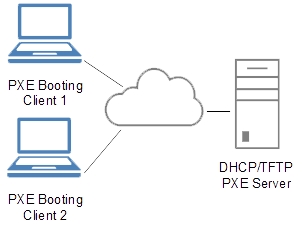
\includegraphics[width=.5\textwidth]{img/PXE_diagram.png}
  \end{center}
  \caption{PXE WorkFlow}
  \label{fig:pxeWork}
\end{figure}

PXE工作流程图:
\begin{figure}[htbp]
  \begin{center}
    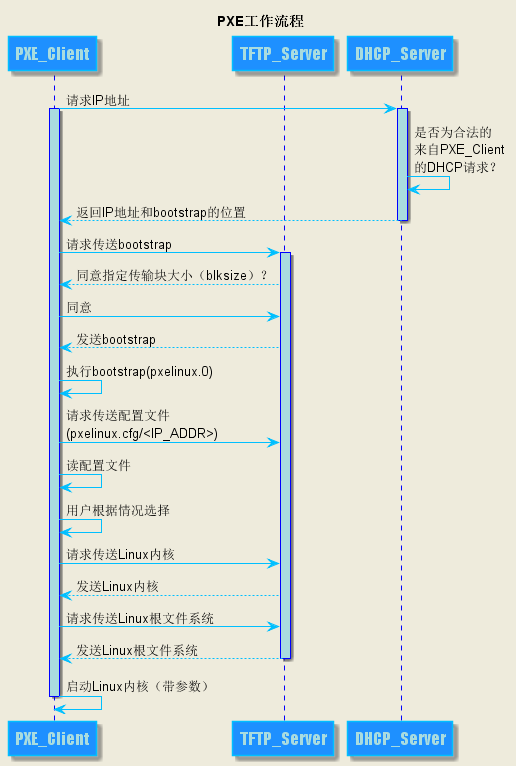
\includegraphics[width=.55\textwidth]{img/pxe01.png}
  \end{center}
  \caption{PXE工作流程图}
  \label{fig:pxeWorkFlow}
\end{figure}

\subsection{安装相关软件包}

\small{
\begin{verbatim}
	rpm -ivh dhcpdxxx
	rpm -ivh nfs-utilsxxx
	rpm -ivh tftp-serverxxx
	rpm -ivh xinetdxxx
	rpm -ivh httpdxxx
	rpm -ivh syslinuxxxx
	rpm -ivh system-config-kickstartxxx
\end{verbatim}
}
\normalsize

\small{
\begin{verbatim}
 # chkconfig tftp on
   # chkconfig xinetd on
\end{verbatim}
}
\normalsize
   
3. Stop some services, such as selinux, iptables
   setenforce 0
or  vi /etc/sysconfig/selinux disabled
    service iptables stop

4. Copy the related files to the related path

\small{
\begin{verbatim}
# mount /dev/cdrom /media
# mkdir /var/ftp/pub/RedHat
# cp -a /media/* /var/ftp/pub/RedHat
# cp /usr/share/syslinux/pxelinux.0 /tftpboot
# cp /var/ftp/pub/RedHat/isolinux/vmlinuz /tftpboot
# cp /var/ftp/pub/RedHat/isolinux/initrd.img /tftpboot
# mkdir /tftpboot/pxelinux.cfg
# vi /tftpboot/pxelinux.cfg/default 
     default install
     prompt 1
     timeout 60
     label local
	localhost	1
     label install
	kernel vmlinuz
	append initrd=initrd.img ramdisk_size=8192 ks=http://192.168.0.254/ks/ks.conf
\end{verbatim}
}
\normalsize

\small{
\begin{verbatim}
   # mount /dev/cdrom /media
   # mkdir /var/ftp/pub/RedHat
   # cp -a /media/* /var/ftp/pub/CentOS
   # cp /usr/share/syslinux/pxelinux.0 /var/lib/tftpboot
   # cp /var/ftp/pub/CentOS/isolinux/vmlinuz /var/lib/tftpboot
   # cp /var/ftp/pub/CentOS/isolinux/initrd.img /var/lib/tftpboot
   # mkdir /var/lib/tftpboot/pxelinux.cfg
   # vi /var/lib/tftpboot/pxelinux.cfg/default
	default install
	prompt 1
	timeout 60
	label local
		localhost	1
	label install
		kernel vmlinuz
		append initrd=initrd.img ramdisk_size=8192 ks=http://192.168.0.254/ks/ks.conf
\end{verbatim}
}
\normalsize

5. Modify the related configure files

\small{
\begin{verbatim}
# vi /etc/dhcp/dhcpd.conf
......
......
next-server	ip_addr;
filename	"pxelinux.0";
......

# vi /etc/http/conf/httpd.conf
Allow from all
# chown -R apache.apache /var/www

# vi /etc/exports
/var/ftp/pub/RedHat 192.168.0.0/255.255.255.0(ro,sync)
\end{verbatim}
}
\normalsize

6. Start services, and later the client can install OS

\small{
\begin{verbatim}
   # service xinetd restart
   # service nfs restart
   # service vsftpd restart
   # service httpd restart
   # service dhcpd restart
\end{verbatim}
}
\normalsize

\begin{verbatim}
NOTE:
In the ks.cfg, the keyword 
clearpart --none is default
change this into:
clearpart --all
\end{verbatim}

%%% Local Variables:
%%% mode: latex
%%% TeX-master: t
%%% End:


\chapter{Samba}

\chapter{Apache}
\label{chap:apache}

Apache HTTP Server是Apache软件基金会的一个开源Web服务器,可以在大多数操
作系统中运行,由于其多平台和安全性被广泛使用,是最流行的Web服务器软件之
一。

Apache支持许多特性,而这些特性大部分通过编译的模块实现。这些特性从服务
器端的编程语言支持到身份认证方案等包括目前所有流行的Web服务器应用。由
于Apache良好的开放性,目前也有很多非官方的模块用以满足某些特殊的应用,
在Apache 2.x中默认包含的模块如表所示:

\section{安装及配置Apache}
\label{subsec:InstallApache}

%%% Local Variables:
%%% mode: latex
%%% TeX-master: t
%%% End:


\chapter{Nginx}
\label{chap:nginx}

\section{关于Nginx}
\label{subsec:AboutNginx}

Nginx是由俄罗斯人Igor Sysoev为俄罗斯访问量第二Rambler.ru站
点开发的,它已经在该站点运行超过两年半了。它的发音为“engine
X”, 是一个高性能的HTTP和反向代理服务器,同时也是一个IMAP/POP3/SMTP 代
理服务器。Igor Sysoev在建立的项目时,使
用基于BSD许可。自Nginx发布四年来,Nginx已经因为它的稳定性、丰富的功能
集、示例配置文件和低系统资源的消耗而闻名。

在俄罗斯许多大网站都已经使用它,且一直表现不凡。截至2007年4月,俄罗斯
大约有20\%左右的虚拟主机是由Nignx服务或代理的。Google在线安全博客中统
计Nginx服务或代理了大约所有Internet虚拟主机的4\%。而Netcraft的统计显
示,Nginx服务的主机在过去的一年里以四倍的速度增长并且在这几年里,它的排
名还在不断上升,下图为Netcraft截止至2010年5月的统计。

\section{Nginx的安装与启动}
\label{subsec:InstallAndStartNginx}

Linux下安装软件有三种方式,这里我以源代码编译安装为主。服务器最小化安装
后,安装依赖包。

\begin{verbatim}
yum install -y pcre-devel \
gcc \
zlib-devel \
openssl-devel
\end{verbatim}

出于管理和安全的目的,我们希望使用一个指定的普通用户身份去运行我们的
Web服务器。所以,我们首先增加一个普通用户用于运行我们的Nginx。

\begin{verbatim}
groupadd nginx
useradd -g nginx nginx
\end{verbatim}

\begin{verbatim}
service iptables stop
chkconfig iptables off
\end{verbatim}

然后下载、解压并编译安装我们的Nginx,

\begin{verbatim}
wget http://nginx.org/download/nginx-1.8.0.tar.gz
tar -xf nginx-1.8.0.tar.gz -C /usr/local/src
cd /usr/local/src/nginx-1.8.0
./configure --user=nginx \
> --group=nginx \
> --with-http_ssl_module \
> --with-http_sub_module
\end{verbatim}

安装过程比较简单,./configure过程会报出一些依赖关系,这里已经解决。下面
来看看./configure后面几个常用的参数:

\begin{verbatim}
--prefix=<dir>         指定安装主目录,默认为/usr/local/nginx
--user=<user>          指定用户身份,如果没有指定则默认使用nobody
--group=<group>        指定组身份
--with-http_ssl_module 启用https支持
\end{verbatim}

\section{Nginx的基本配置}
\label{subsec:NginxConf}

Linux下基本上每个服务都会有它的主配置文件,该文件会定义服务应该如果去运
行,使用些什么参数,启用些什么功能,相关会涉及到的一些操作文件在哪,所
以主配置文件对服务是至关重要的。下面我们来分析一下Nginx的主配置文件。

\subsection{Nginx主配置概述}

Linux下基本上每个服务都会有它的主配置文件,该文件会定义服务应该如果去运
行,使用些什么参数,启用些什么功能,相关会涉及到的一些操作文件在哪,所以主
配置文件对服务是至关重要的。Nginx的主配置文件默认情况下位于
/usr/local/nginx/conf/nginx.conf,以下为Nginx配置文件一些参数的注释。

\begin{verbatim}
#user nobody;
#指定使用的用户
worker_processes 1;
#开启的进程数,一般设置 1-5
#error_log logs/error.log;
#error_log logs/error.log notice;
#error_log logs/error.log info;
#定义错误日志,以及记录的日志等级
#pid
logs/nginx.pid;
#定义 pid 文件位置
events {
# use [ kqueue | rtsig | epoll | /dev/poll | select | poll ];
#use epoll; #使用 epoll(linux2.6 的高性能方式)
#Nginx 支持如下处理连接的方法(I/O 复用方法),这些方法可以通过 use 指令指定。
#select - 标准方法。 如果当前平台没有更有效的方法,它是编译时默认的方法。你可以使用配置参
数 –with-select_module 和 –without-select_module 来启用或禁用这个模块。
#poll - 标准方法。 如果当前平台没有更有效的方法,它是编译时默认的方法。你可以使用配置参数
–with-poll_module 和 –without-poll_module 来启用或禁用这个模块。
#kqueue - 高效的方法,使用于 FreeBSD 4.1+, OpenBSD 2.9+, NetBSD 2.0 和 MacOS X. 使用双
处理器的 MacOS X 系统使用 kqueue 可能会造成内核崩溃。
#epoll - 高效的方法,使用于 Linux 内核 2.6 版本及以后的系统。在某些发行版本中,如 SuSE 8.2,
有让 2.4 版本的内核支持 epoll 的补丁。
#rtsig - 可执行的实时信号,使用于 Linux 内核版本 2.2.19 以后的系统。可是从 Linux 内核版本
2.6.6-mm2 开始,这个参数就不再使用了.
#/dev/poll - 高效的方法,使用于 Solaris 7 11/99+, HP/UX 11.22+ (eventport), IRIX 6.5.15+ 和
Tru64 UNIX 5.1A+.
#eventport - 高效的方法,使用于 Solaris 10. 为了防止出现内核崩溃的问题, 有必要安装这个安全补丁。
worker_connections 1024;
#worker_connections 51200; #每个进程最大连接数(最大连接=连接数 x 进程数)
}
http {
include
mime.types;
#文件扩展名与文件类型映射表
default_type application/octet-stream;
#默认文件类型
#log_format main '$remote_addr - $remote_user [$time_local] "$request" '
# '$status $body_bytes_sent "$http_referer" '
# '"$http_user_agent" "$http_x_forwarded_for"';
#access_log logs/access.log main;
sendfile
on;
#开启高效文件传输模式
#tcp_nopush
on;
#该选项用于防止网络阻塞
#keepalive_timeout 0;
keepalive_timeout 65;
##长链接超时时间
#gzip on;
#打开 gzip 压缩
#fastcgi_connect_timeout 300;
#fastcgi_send_timeout 300;
#fastcgi_read_timeout 300;
#fastcgi_buffer_size 128k;
#fastcgi_buffers 4 256k;
#fastcgi_busy_buffers_size 256k;
#fastcgi_temp_file_write_size 256k;
#fastcgi_temp_path /dev/shm;
#fastcgi 连接超时时间和缓存
server {
listen
80;
server_name localhost;
#主机名
#charset koi8-r;
#默认字符编码 charset gb2312
#access_log logs/host.access.log main;
location / {
#pass 路径匹配 能够匹配路径中带“/”的 不过需要注意的是如果之后也有相关“/”匹配项并且
使用比此处更精确匹配符,则以之后表达式优先
root html;
index index.html index.htm;
}
#error_page 404
/404.html;
# redirect server error pages to the static page /50x.html
#
error_page 500 502 503 504 /50x.html;
location = /50x.html {
#精确的匹配,并且不再向下匹配
root html;
}
#
#location ~ \.php$ {
#正则表达式匹配 一旦匹配则不再向下匹配
#
proxy_pass http://127.0.0.1;
#}
# pass the PHP scripts to FastCGI server listening on 127.0.0.1:9000
#
#location ~ \.php$ {
# root
html;
# fastcgi_pass 127.0.0.1:9000;
#指定 fastcgi 的地址端口
# fastcgi_index index.php;
# fastcgi_param SCRIPT_FILENAME /scripts$fastcgi_script_name;
# include fastcgi_params;
#}
# deny access to .htaccess files, if Apache's document root
# concurs with nginx's one
#
#location ~ /\.ht {
#
deny all;
#不允许访问以.ht 开头的文件
#}
}
# another virtual host using mix of IP-, name-, and port-based configuration
#
#server {
# listen
8000;
# listen
somename:8080;
# server_name somename alias another.alias;
# location / {
# root html;
# index index.html index.htm;
#
}
#}
#以上在配置虚拟主机
# HTTPS server
#
#server {
# listen 443;
# server_name localhost;
# ssl on;
# ssl_certificate cert.pem;
# ssl_certificate_key cert.key;
# ssl_session_timeout 5m;
# ssl_protocols SSLv2 SSLv3 TLSv1;
# ssl_ciphers ALL:!ADH:!EXPORT56:RC4+RSA:+HIGH:+MEDIUM:+LOW:+SSLv2:+EXP;
# ssl_prefer_server_ciphers on;

#以上为 ssl 配置
# location / {
# root html;
# index index.html index.htm;
# }
# }
}
\end{verbatim}

\subsection{Nginx虚拟主机配置}

利用虚拟主机技术,可以把一台真正的主机分成许多虚拟的主机,每一台虚拟主
机都具有独立的域名和IP地址,具有完整的Internet服务器(www,FTP,email)
功能。虚拟主机之间完全独立,在外界看来,每一台虚拟主机和一台独立的主机
完全一样。效果一样但费用却大不一样了。由于多台虚拟主机共享一台真实主机
的资源,每个虚拟主机用户承受的硬件费用、网络维护费用、通信线路的费用均
大幅度降低,Internet真正成为人人用得起的网络!

虚拟主机共分为三种:基于IP的虚拟主机,基于端口的虚拟主机和基于名称的虚拟
主机。前两种由于受到成本和客户使用习惯的限制,相对使用的没有基于名称的
虚拟主机多,以下我们介绍一下三种虚拟主机的配置。

\subsection{安全的连接https}

众所周知,我们在互联网上冲浪,一般使用的是http协议(超文本传输协议),
默认情况下数据是明文传送的,这些数据在传输过程中都可能会被捕获和窃听,
因此是不安全的。https可以说是http协议的安全版,就是为了满足对安全性要求
比较高的用户而设计的。

\section{Nginx日志管理}

\section{Nginx访问控制}

\section{Nginx反向代理}
\label{subsec:NginxReverseProxy}

反向代理(Reverse Proxy)方式是指以代理服务器来接受Internet上的连接请求,
然后将请求转发给内部网络上的服务器,并将从服务器上得到的结果返回
给Internet上请求连接的 客户端,此时代理服务器对外就表现为一个服务器。

反向代理又称为Web服务器加速,是针对Web服务器提供加速功能的。它作为代
理Cache,但并不针对浏览器用户,而针对一台或多台特定Web服务器(这也是反
向代理名称的由来)。代理服务器可以缓存一些web的页面,降低了web服务器的
访问量,所以可以降低web服务器的负载。web服务器同时处理的请求数少了,响
应时间自然就快了。同时代理服务器也存了一些页面,可以直接返回给客户端,
加速客户端浏览。实施反向代理,只要将反向代理设备放置在一台或多台Web服务
器前端即可。当互联网用户访问某个WEB服务器时,通过DNS服务器解析后的IP地
址是代理服务器的IP地址,而非原始Web服务器的IP地址,这时代理服务器设备充
当Web服务器,浏览器可以与它连接,无需再直接与Web服务器相连。因此,大
量Web服务工作量被转载到反向代理服务上。不但能够很大程度上减轻web服务器
的负担,提高访问速度,而且能够防止外部网主机直接和web服务器直接通信带来
的安全隐患。

\begin{figure}[!h]
  \centering
  \subfloat[squid代理模式]{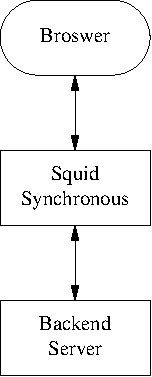
\includegraphics[width=.2\textwidth]{graph/reverse_squid.pdf}}\hspace{30pt}
  \subfloat[nginx代理模式]{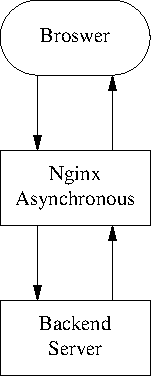
\includegraphics[width=.2\textwidth]{graph/reverse_nginx.pdf}}
  \caption{两种代理模式比较}
  \label{fig:squidVSnginx}
\end{figure}

squid同步传输:浏览器发起请求,而后请求会立刻被转到后台,于是在浏览器和
后台之间就建立了一个通道。在请求发起直到请求完成,这条通道都是一直存在
的。

nginx异步传输:浏览器发起请求,请求不会立刻转到后台,而是将请求数据(
header )先收到nginx上,然后nginx再把这个请求发到后端, 后端处理完之后把数
据返回到nginx上, nginx将数据流发到浏览器,这点和lighttpd有点不同,
lighttpd是将后端数据完全接收后才发送到浏览器。

那么这到底有什么好处呢?

\begin{enumerate}[itemsep=0pt,parsep=0pt]
\item 假设用户执行一个上传文件操作,因为用户网速又比较慢,因此需要花半
  个小时才能把文件传到服务器。squid的同步代理在用户开始上传后就和后台建
  立了连接,半小时后文件上传结束,由此可见,后台服务器连接保持了半个小
  时;而 nginx异步代理就是先将此文件收到nginx上,因此仅仅是nginx和用户
  保持了半小时连接,后台服务器在这半小时内没有为这个请求开启连接,半小
  时后用户上传结束,nginx才将上传内容发到后台,nginx和后台之间的带宽是
  很充裕的,所以只花了一秒钟就将请求发送到了后台,由此可见,后台服务器
  连接保持了一秒。同步传输花了后台服务器半个小时,异步传输只花一秒,可
  见优化程度很大。

\item 在上面这个例子中,假如后台服务器因为种种原因重启了,上传文件就自
  然中断了,这对用户来说是非常恼火的一件事情,想必我们也有上传文件传到
  一半被中断的经历。用nginx代理之后,后台服务器的重启对用户上传的影响减
  少到了极点,而nginx是非常稳定的并不需要常去重启它,即使需要重启,利用
  kill -HUP就可以做到不间断重启nginx。

\item 异步传输可以令负载均衡器更有保障,为什么这么说呢?在其它的均衡器
  ( lvs/haproxy/apache 等)里,每个请求都是只有一次机会的,假如用户发起
  一个请求,结果该请求分到的后台服务器刚好挂掉了,那么这个请求就失败了;
  而 nginx因为是异步的,所以这个请求可以重新发往下一个后台,下一个后台
  返回了正常的数据,于是这个请求就能成功了。还是用用户上传文件这个例子,
  假如不但用了nginx代理,而且用了负载均衡,nginx把上传文件发往其中一台
  后台,但这台服务器突然重启了,nginx收到错误后,会将这个上传文件发到另
  一台后台,于是用户就不用再花半小时上传一遍。

\item 假如用户上传一个10GB大小的文件,而后台服务器没有考虑到这个情况,
  那么后台服务器岂不要崩溃了。用nginx就可以把这些东西都拦在nginx上, 通
  过nginx的上传文件大小限制功能来限制,另外nginx性能非常有保障,就放心
  的让互联网上那些另类的用户和nginx对抗去吧。
\end{enumerate}

\subsection{Nginx 与 Lua 结合}

%%% Local Variables:
%%% mode: latex
%%% TeX-master: t
%%% End:


\chapter{LAMP}

\section{安装依赖包}

Needless to say, you should install required system packages. So you
cancontinue the next steps. :-)

Be sure these packages are installed:

\small{
\begin{verbatim}
  gcc
  gcc-c++
  flex
  bison
  autoconf
  automake
  bzip2-devel
  ncurses-devel
  libjpeg-devel
  libpng-devel
  libtiff-devel
  freetype-devel
  pam-devel
\end{verbatim}
}
\normalsize

\section{安装额外的包}

In this section, we need to compile and install four packages:

\begin{enumerate}[itemsep=0pt,parsep=0pt]
\item GD2
  \small{
\begin{verbatim}
  [root@lamp ~] # cd /usr/local/src
  [root@lamp src] # tar xzvf gd-2.0.34.tar.gz
  [root@lamp src] # cd gd-2.0.34
  [root@lamp gd-2.0.34] # ./configure --prefix=/usr/local/gd2
  [root@lamp gd-2.0.34] # make
  [root@lamp gd-2.0.34] # make install  
\end{verbatim}
  }
  \normalsize

\item LibXML2
  \small{
\begin{verbatim}
  [root@lamp ~] # cd /usr/local/src
  [root@lamp src] # tar xzvf libxml2-2.6.29.tar.gz
  [root@lamp src] # cd libxml2-2.6.29
  [root@lamp libxml2-2.6.29] # ./configure --prefix=/usr/local/libxml2
  [root@lamp libxml2-2.6.29] # make
  [root@lamp libxml2-2.6.29] # make install
\end{verbatim}
  }
  \normalsize

\item LibMcrypt
  \small{
\begin{verbatim}
  [root@lamp ~] # cd /usr/local/src
  [root@lamp src] # tar xjvf libmcrypt-2.5.8.tar.bz2
  [root@lamp src] # cd libmcrypt-2.5.8
  [root@lamp libmcrypt-2.5.8] # ./configure --prefix=/usr/local/libmcrypt
  [root@lamp libmcrypt-2.5.8] # make
  [root@lamp libmcrypt-2.5.8] # make install
\end{verbatim}
  }
  \normalsize

\item OpenSSL
  \small{
\begin{verbatim}
  [root@lamp ~] # cd /usr/local/src
  [root@lamp src] # tar xzvf openssl-0.9.8e.tar.gz
  [root@lamp src] # cd openssl-0.9.8e
  [root@lamp openssl-0.9.8e] # ./config --prefix=/usr/local/openssl
  [root@lamp openssl-0.9.8e] # make
  [root@lamp openssl-0.9.8e] # make test
  [root@lamp openssl-0.9.8e] # make install
\end{verbatim}
  }
  \normalsize

\end{enumerate}

\section{编译安装MySQL}

\small{
\begin{verbatim}
  [root@lamp ~] #tar xzvf mysql-5.0.27.tar.gz
  [root@lamp ~] # cd mysql-5.0.27
  [root@lamp mysql-5.0.27] # ./configure \
  "--prefix=/usr/local/mysql" \
  "--localstatedir=/var/lib/mysql" \
  "--with-mysqld-user=mysql" \
  "--without-debug" \
  "--with-big-tables" \
  "--with-extra-charsets=all" \
  "--with-pthread" \
  "--enable-static" \
  "--enable-thread-safe-client" \
  "--with-client-ldflags=-all-static" \
  "--with-mysqld-ldflags=-all-static" \
  "--enable-assembler" \
  "--without-isam" \
  "--without-innodb" \
  "--without-ndb-debug"
  
  [root@lamp msyql-5.0.27] # make
  [root@lamp mysql-5.0.27] # make install
  [root@lamp mysql-5.0.27] # useradd mysql
  [root@lamp mysql-5.0.27] # cd /usr/local/mysql
  [root@lamp mysql] # bin/mysql_install_db --user=mysql
  [root@lamp mysql] # chown -R root:mysql .
  [root@lamp mysql] # chown -R mysql /var/lib/mysql
  [root@lamp mysql] # cp share/mysql/my-huge.cnf /etc/my.cnf
  [root@lamp mysql] # cp share/mysql/mysql.server /etc/rc.d/init.d/mysqld
  [root@lamp mysql] # chmod 755 /etc/rc.d/init.d/mysqld
  [root@lamp mysql] # chkconfig --add mysqld
  [root@lamp mysql] # chkconfig --level 3 mysqld on
  [root@lamp mysql] # /etc/rc.d/init.d/mysqld start
  [root@lamp mysql] # bin/mysqladmin -u root password 'clear123'
\end{verbatim}
}
\normalsize

\section{编译安装Apache}

\small{
\begin{verbatim}
  [root@lamp src] # cd /usr/local/src
  [root@lamp src] # tar xjvf httpd-2.2.4.tar.bz2
  [root@lamp src] # cd httpd-2.2.4
  [root@lamp httpd-2.2.4] # ./configure \
  "--prefix=/usr/local/apache2" \
  "--with-included-apr" \
  "--enable-so" \
  "--enable-deflate=shared" \
  "--enable-expires=shared" \
  "--enable-rewrite=shared" \
  "--enable-static-support" \
  "--disable-userdir"
  [root@lamp httpd2.2.4] # make
  [root@lamp httpd2.2.4] # make install
  [root@lamp httpd2.2.4] # echo '/usr/local/apache2/bin/apachectl start' \
  > >> /etc/rc.local
\end{verbatim}
}
\normalsize

\section{编译安装PHP}

\small{
\begin{verbatim}
  [root@lamp ~] # cd /usr/local/src
  [root@lamp src] # tar xjvf php-5.2.3.tar.bz2
  [root@lamp php-5.2.3] # cd php-5.2.3
  [root@lamp php-5.2.3] # ./configure \
  "--prefix=/usr/local/php" \
  "--with-apxs2=/usr/local/apache2/bin/apxs" \
  "--with-config-file-path=/usr/local/php/etc" \
  "--with-mysql=/usr/local/mysql" \
  "--with-libxml-dir=/usr/local/libxml2" \
  "--with-gd=/usr/local/gd2" \
  "--with-jpeg-dir" \
  "--with-png-dir" \
  "--with-bz2" \
  "--with-freetype-dir" \
  "--with-iconv-dir" \
  "--with-zlib-dir " \
  "--with-openssl=/usr/local/openssl" \
  "--with-mcrypt=/usr/local/libmcrypt" \
  "--enable-soap" \
  "--enable-gd-native-ttf" \
  "--enable-memory-limit" \
  "--enable-ftp" \
  "--enable-mbstring" \
  "--enable-exif" \
  "--disable-ipv6" \
  "--disable-cgi" \
  "--disable-cli"
  [root@lamp php-5.2.3] # make
  [root@lamp php-5.2.3] # make install
  [root@lamp php-5.2.3] # mkdir /usr/local/php/etc
  [root@lamp php-5.2.3] # cp php.ini-dist /usr/local/php/etc/php.ini
\end{verbatim}
}
\normalsize

\section{安装Zend加速器}

\small{
\begin{verbatim}
  [root@lamp ~]# cd /usr/local/src
  [root@lamp ~]# tar xf ZendOptimizer-3.2.8-linux-glibc21-i386.tar.gz
  [root@lamp ~]# ./ZendOptimizer-3.2.8-linux-glibc21-i386/install.sh
\end{verbatim}
}
\normalsize

\section{整合Apache与PHP}

We should modify configure file httpd.conf:

\small{
\begin{verbatim}
[root@lamp ~]# emacs /usr/local/apache2/conf/httpd.conf
\end{verbatim}
}
\normalsize

Find this line,

\small{
\begin{verbatim}
AddType application/x-gzip .gz .tgz
\end{verbatim}
}
\normalsize

Add on line under this line,

\small{
\begin{verbatim}
AddType application/x-httpd-php .php
\end{verbatim}
}
\normalsize

Find these lines,

\small{
\begin{verbatim}
<IfModule dir_module>
DirectoryIndex index.html
<IfModule>
\end{verbatim}
}
\normalsize

Change them like this,

\small{
\begin{verbatim}
<IfModule dir_module>
DirectoryIndex index.html index.htm index.php
<IfModule>
\end{verbatim}
}
\normalsize

Find these lines and uncomment them,

\small{
\begin{verbatim}
#Include conf/extra/httpd-mpm.conf
#Include conf/extra/httpd-info.conf
#Include conf/extra/httpd-vhosts.conf
#Include conf/extra/httpd-default.conf
\end{verbatim}
}
\normalsize

When finished, save it! Then restart apache service,

\small{
\begin{verbatim}
[root@lamp ~]# /usr/local/apache2/bin/apachectl restart
\end{verbatim}
}
\normalsize

%%% Local Variables:
%%% mode: latex
%%% TeX-master: t
%%% End:


\chapter{多网卡绑定bonding}

Linux bonding提供将多个网络接口设备捆绑为单个网络接口设置来使用,用于网
络负载均衡及网络冗余。

以太网平衡设备即使用两个或两个以上的网络接口模拟一个虚拟的网络接口用以
外部网络连接。这多个真实网络接口可以连接在同一交换设备或多个交换设备上,
以达到多通路高可用性。在所有真实网络接口中可以指定其中某些真实网络接口
活跃,其他真实网络接口在活跃的真实网络接口故障时接管网络传输;也可以指
定所有真实网络接口活跃,分担全部网络传输带宽。
 
通道绑定(Channel bonding)需要服务器至少拥有2个以太网卡,当使用绑定功能
的时候,bonding模块会使用第一个实际网卡的MAC地址来通信,在侦测到这个网
卡失败以后,它会把这个MAC地址指定到另一块网卡上。

\section{bonding的几种模式}

bonding只能提供链路监测,即从主机到交换机的链路是否接通。如果只是交换机
对外的链路down掉了,而交换机本身并没有故障,那么bonding会认为链路没有问
题而继续使用。
 
miimon是用来进行链路监测的。 比如:miimon=100,那么系统每100ms监测一次链
路连接状态,如果有一条线路不通就转入另一条线路;mode的值表示工作模式,
他共有0,1,2,3,4,5,6七种模式,作者遇到的场景是使用的1,0,6三种,
其他场景适合哪些模式作者也不清楚。
 
mode=1,表示fault-tolerance (active-backup)提供网络冗余功能,工作方式是
主备模式,也就是说默认情况下只有一块网卡工作,另一块做备份。
 
mode=0,表示load balancing (round-robin)为负载均衡模式,两块网卡都工作,
但是与网卡相连的交换机必须做特殊配置( 这两个端口应该采取聚合方式),因
为做bonding的这两块网卡是使用同一个MAC地址。
 
mode=6,表示load balancing (round-robin)为负载均衡方式,两块网卡都工作,
但是该模式下无需配置交换机,因为做bonding的这两块网卡是使用不同的MAC地
址。
 
\section{RHEL下配置bonding}

华为RH1288服务器共有8块网卡,eth0与eth1做bond0,对应管理网
段172.16.25.X,主备模式;eth2与eth3做bond1,此网段暂没有配置IP信息,主
备模式;eth4与eth5做bond2,对应存储网段10.10.2.X,主备模式。

编辑/etc/modprobe.d/dist.conf文件,在文件末尾添加如下几行,开
启bonding功能\footnote{这是RHEL6U4的系统,如果是RHEL5系列的机器,配置文
  件则为/etc/modprobe.conf}。

\begin{verbatim}
# vim /etc/modprobe.d/dist.conf
alias bond0 bonding
options bond0 mode=1 miimon=100

alias bond1 bonding
options bond1 mode=1 miimon=100

alias bond2 bonding
options bond2 mode=1 miimon=100
\end{verbatim}

编辑虚拟网络接口配置文件bond0,

\begin{verbatim}
# vim /etc/sysconfig/network-scripts/ifcfg-bond0
DEVICE=bond0
ONBOOT=yes
BOOTPROTO=none
NETWORK=
IPADDR=
NETMASK=
GATEWAY=
USERCTL=no
\end{verbatim}

分别编辑eth0与eth1网络接口文件ifcfg-eth0与ifcfg-eth1,

\begin{verbatim}
# vim /etc/sysconfig/network-scripts/ifcfg-eth0
DEVICE=eth0
BOOTPROTO=none
TYPE=Ethernet
ONBOOT=yes
USERCTL=no
MASTER=bond0 
SLAVE=yes

# vim /etc/sysconfig/network-scripts/ifcfg-eth1
DEVICE=eth1
BOOTPROTO=none
TYPE=Ethernet
ONBOOT=yes
USERCTL=no
MASTER=bond0 
SLAVE=yes
\end{verbatim}

由于该机器对应的交换机接口为VLAN 210,所以,需要在bond0接口上配置VLAN。

\begin{verbatim}
# vconfig add bond0 210
\end{verbatim}

这样就产生了一个bond0.210的虚拟网络接口,这样就可以启用该接口,并配
置IP信息,

\begin{verbatim}
# ifconfig bond0.210 up
# vim /etc/sysconfig/network-scripts/ifcfg-bond0.210
DEVICE=bond0.210
BOOTPROTO=none
ONBOOT=yes
USERCTL=no
IPADDR=172.16.25.93
NETMASK=255.255.255.0
GATEWAY=172.16.25.254
VLAN=yes
\end{verbatim}

查看上面已配置的VLAN信息,

\begin{verbatim}
# cat /proc/net/vlan/config
VLAN Dev name	 | VLAN ID
Name-Type: VLAN_NAME_TYPE_RAW_PLUS_VID_NO_PAD
bond0.210      | 210  | bond0

# cat /proc/net/vlan/bond0.210 
bond0.210  VID: 210	 REORDER_HDR: 1  dev->priv_flags: 1
         total frames received         4663
          total bytes received       224809
      Broadcast/Multicast Rcvd          38

      total frames transmitted          228
       total bytes transmitted         44140
            total headroom inc           0
           total encap on xmit            0
Device: bond0
INGRESS priority mappings: 0:0  1:0  2:0  3:0  4:0  5:0  6:0 7:0
EGRESS priority mappings:
\end{verbatim}

\section{SuSE下配置bonding}

bond0配置:

\begin{verbatim}
# cat /etc/sysconfig/network/ifcfg-bond0
DEVICE='bond0'
ONBOOT='yes'
BOOTPROTO='static'
IPADDR='0.0.0.0/24'   
STARTMODE='auto'
BONDING_MASTER='yes'
BONDING_MODULE_OPTS='mode=1 miimon=100'
BONDING_SLAVE0='eth0'
BONDING_SLAVE1='eth1'
USERCONTROL='no'
\end{verbatim}

br0配置:

\begin{verbatim}
# cat /etc/sysconfig/network/ifcfg-br0
BOOTPROTO='static'
BRIDGE='yes'
BRIDGE_FORWARDDELAY='0'
BRIDGE_PORTS='bond1'
BRIDGE_STP='off'
IPADDR='0.0.0.0/24'    	##管理网ip
STARTMODE='auto'
USERCONTROL='no'

# cat /etc/sysconfig/network/ifcfg-vlan0     ##为网卡打Vlan Tag
BOOTPROTO='static'
ETHERDEVICE='br0'
IPADDR='145.240.21.11/24'
STARTMODE='auto'
USERCONTROL='no'
VLAN_ID='210'                       ##上联核心交换机端口的Vlan号

# cat /proc/net/vlan/config         ##验证Vlan是否设置成功
VLAN Dev name | VLAN ID
Name-Type: VLAN_NAME_TYPE_RAW_PLUS_VID_NO_PAD
vlan0         | 210 | br0
\end{verbatim}

\section{单网卡多IP配置}
\label{sec:SingleCardMultiIP}

% \chapter{LVM硬盘管理及扩容}

% LVM是 Logical Volume Manager(逻辑卷管理)的简写,它由Heinz Mauelshagen在
% Linux 2.4内核上实现。LVM将一个或多个硬盘的分区在逻辑上集合,相当于一个
% 大硬盘来使用,当硬盘的空间不够使用的时候,可以继续将其它的硬盘的分区加
% 入其 中,这样可以实现磁盘空间的动态管理,相对于普通的磁盘分区有很大的灵
% 活性。
 
% 与传统的磁盘与分区相比,LVM为计算机提供了更高层次的 磁盘存储。它使系统
% 管理员可以更方便的为应用与用户分配存储空间。在LVM管理下的存储卷可以按需
% 要随时改变大小与移除(可能需对文件系统工具进行升 级)。LVM也允许按用户组
% 对存储卷进行管理,允许管理员用更直观的名称(如"sales'、 'development')代
% 替物理磁盘名(如'sda'、'sdb')来标识存储卷。
 
% 如图所示LVM模型:
 
% 由四个磁盘分区可以组成一个很大的空间,然后在这些空间上划分一些逻辑分区,
% 当一个逻辑分区的空间不够用的时候,可以从剩余空间上划分一些空间给空间不
% 够用的分区使用。

% \chapter{使用U盘安装Gnu系统}

% 使用U盘安装系统在某些时候还是很方便的,其安装速度也是蛮给力的。为什么会
% 有本章内容呢?主要是小白在装机中发现有的机器不带光驱,而且身边也没有移
% 动光驱可用,并且也不能从网络启动来安装系统。由于这些诸多限制,小白就想
% 可不可以使用U盘安装呢?网上搜索了一下,果然可以,而且安装速度比光驱快!
% 下面就介绍一下如何使用U盘来安装Gnu/Linux系统。

% \section{准备工作}

% \begin{enumerate}[itemsep=0pt,parsep=0pt]
% \item 4G以上的优盘,格式化成FAT32
% \item 镜像编辑软件UltraISO
% \item Gnu/Linux镜像文件
% \end{enumerate}

% \section{制作启动盘}

% \begin{enumerate}[itemsep=0pt,parsep=0pt]
% \item 启动软件后打开Linux ISO文件
% \item 点击“工具”,“加载到虚拟光驱”,点击“加载”
% \item 打开“我的电脑”找到虚拟光驱的盘符 
% \item 找到“boot.ISO”文件,双击打开
% \item 点击“启动”,“写入硬盘镜像”
% \item 选择你的U盘,写入方式:USB-HDD+,点击“写入”,开始写入引导文件到
%   U盘
% \item 等待一会儿,消息栏提示“刻录成功”,引导文件写入完毕
% \item 确认是否写入成功和盘符是否选对:打开“我的电脑”,可移动存储栏里
%   出现 以:“Red Hat Ent”命名的盘符,代表写入成功
% \end{enumerate}

% \section{开始安装Gnu/Linux}

% 在安装过程中,需要选择Grub安装位置时,需要注意一下,我们要把Grub安装到
% 系统盘中,默认是安装在U盘里的,这时可以修改之以继续安装。如果这一步没有
% 修改,也没有关系,等系统安装完毕重启时,不要拔掉U盘。一切就绪进入系统后,
% 可以使用grub-install命令重新安装Grub到指定的盘中。

\chapter{RAID技术}

RAID技术有各种级别之分,包括RAID0、RAID1、RAID2、RAID3、RAID4、RAID5、
RAID5E、RAID5EE、RAID6、RAID10等。作者接触最多的是RAID0、RAID1、RAID5及
RAID10这些RAID级别,其他级别在实际工作当中并没有见到,这里就不在介绍。

\section{RAID基础知识}

RAID最初是1987年在加利福尼亚大学进行的一个科研项目,后来由伯克利分校的
D.A. Patterson教授在1988年正式提出。

RAID是Redundant Array of Inexpensive Disks的缩写,直译为“廉价冗余磁盘阵
列”,最初是为了组合多块小容量的廉价磁盘来代替大容量的昂贵磁盘,同时希望
在磁盘失效时不会对数据造成影响而开发出的一种磁盘存储技术。

后来随着磁盘研发技术的不断提升,硬盘容量越来越大,成本却不断下降,所以
RAID中“Inexpensive(廉价)”一词已经失去意义,于是将这个词用
“Independent(独立)”来替代,RAID就成了”独立冗余磁盘阵列“,也简称为”磁
盘阵列“,但这只是名称的变化,实质性的内容并没有改变。

\subsection{RAID解决了什么问题}

通俗地说,RAID就是通过将多个磁盘按照一定的形式和方案组织起来,通过这样
的形式能够获取比单个磁盘更高的速度、更好的稳定性、更大的存储能力的存储
解决方案,我们不必关心磁盘阵列究竟由多少块磁盘组成,使用中整个整列就如
同一块磁盘一样。所以,RAID技术能够为计算机系统提供以下三个方面的优异性
能:

\begin{enumerate}[itemsep=0pt,parsep=0pt]
\item 提供更大的存储空间
\begin{quote}
  使用RAID技术,就可以把多块磁盘组成一个更大的存储空间供我们使用。比如,
  利用RAID0技术把5块1TB的硬盘组织起来,能够提供5TB的存储空间。
\end{quote}

\item 提供更快的传输速度
\begin{quote}
  著名的摩尔定律告诉我们,CPU的性能每隔18个月就会提高一倍,可见其速度增
  长之快。然而,机械硬盘作为计算机中最重要的存储设备,在容量飞速增长的
  同时,速度却提高缓慢,已经成为计算机速度发展的瓶颈。

  如果采用RAID技术,可以让很多机械硬盘同时传输数据,而这些硬盘在逻辑上
  又表现为一块硬盘,所以使用RAID可以达到单个磁盘几倍、甚至N多倍的速率。
  也就是说,RAID技术可以通过在多个磁盘上同时存储和读取数据的方式来大幅
  提高存储系统的数据吞吐量。
\end{quote}

\item 提高更高的安全性
\begin{quote}
RAID可以通过数据校验提供容错功能,在很多RAID模式中都有较为完备的冗余措
施,甚至是直接相互的镜像备份,从而大大提高来RAID系统的容错性,让系统的
稳定性更好、安全性更高。
\end{quote}
\end{enumerate}

\section{RAID实现方式}

\subsection{RAID0数据组织原理}

RAID0是无冗余、无校验的磁盘阵列,实现RAID0,至少需要两个以上硬盘,它将
两个以上的硬盘合并成一块,数据同时分散在每块磁盘中,因为带宽加倍,所以
读写速度加倍,RAID0的理论速度是单块硬盘的N倍,但是由于数据并不是保存在
一个硬盘上,而是分成数据块保存在不同的硬盘上,所以安全性也下降N倍,只要
任何一块磁盘损坏就会丢失所有数据。

RAID0是最简单的一种RAID形式,目的是把多块物理盘连接在一起形成一个容量更
大的存储设备,RAID0逻辑盘的容量等于物理盘的容量乘以成员盘的数目。

原理图

RAID0只是单纯地提高读写性能,并没有数据的可靠性提供保证,而且其中的任何
一个物理盘失效都将影响到所有数据。因此,RAID0不能用于数据安全性要求高的
场合。
\subsection{RAID1数据组织原理}

RAID1通过磁盘数据镜像实现数据的冗余,在两块磁盘上产生互为备份的数据,当
其中一块成员盘出现故障时,系统还可以从另外一块成员盘中读取数据。因此,
RAID1可以提供更好的冗余性。

RAID1又称为磁盘镜像,需要在两个物理盘共同构建,使用磁盘镜像技术,方法是
在工作磁盘之外再加一额外的备份磁盘,两个磁盘所存储的数据完全一样,数据
写入工作磁盘的同时亦写入备份磁盘,也就是将一块物理盘的内容完全复制到另
一块物理盘上。所以,两块物理盘所构成的RAID1阵列,其容量仅等于一块磁盘的
容量,其数据分布情况如图所示。

原理图

RAID1是磁盘阵列中单位成本最高的,但提供来很高的数据安全性和可用性。当一
个物理盘失效时,系统可以自动切换到镜像盘上读写,而不需要重组失效的数据。

RAID1是所有RAID等级中实现成本最高的一种,尽管如此,我们还是选择RAID1来
保存那些关键性的重要数据。

\subsection{RAID10数据组织原理}

\subsection{RAID5数据组织原理}

\section{MegaRAID Cli工具基本使用}
\label{sec:MegaraidCmd}

我们都是使用过LSI的Web界面去配置RAID,虽听起来很高大上,但整个配置过程
是那么的令人蛋疼。配置完成后,我们还要按“Ctrl+Alt+Del”组合键来重启机
器,步骤虽有些繁琐,但仍能令人接受。MegaRAID Cli工具是在命令行模式下操
作RAID控制器的,它的优点之一就是做完RAID之后,可以直接使用并不需要重
启操作系统,而且操作简单方便。

写这一节的目的并不是推荐使用该工具,而是熟悉了原来的配置界面,不愿意再
学新的东西。若不是同事的提示,还不知有这种很xx的工具,使用起来确实很酷,
愿意跟大家分享一下使用过程。

要想使用该工具,首先系统上要安装相应的软件包,这里省略安装过程。安装完
毕之后,工具默认会安装在/opt/MegaRAID/MegaCli的目录下。

本次使用该命令行工具的场景:新到了两块Intel的SATA接口400GB的SSD硬盘,欲
测其性能。原来的服务器上自带了4块600GB的磁盘并做了RAID10,这四块磁盘分
别占据了第0、1、2、3这四个硬盘插槽,在第4、第5个插槽放置了SSD盘,操作系
统使用的是SLES 11.2。下面是具体的操作过程,

\subsection{制作RAID}

\begin{enumerate}[itemsep=0pt,parsep=0pt]
\item 查看RAID卡的设备号
\begin{verbatim}
# cd /opt/MegaRAID/MegaCli
# ./MegaCli64 -PDList -aAll |grep "Device ID"
Enclosure Device ID: 252
Enclosure Device ID: 252 
Enclosure Device ID: 252
Enclosure Device ID: 252
Enclosure Device ID: 252
Enclosure Device ID: 252
\end{verbatim}

说明:上面的输出,表示我们有一个RAID卡,因为这些ID是一样的。这个卡下面
有6个盘,这里的ID号需要记下来,后面做RAID时需要用到。可以把该RAID的ID号
理解为主设备号。
	
\item 查看Slot ID以确认有无错序的情况
\begin{verbatim}
# ./MegaCli64 -PDList -aAll |grep "Slot"  
Slot Number: 0
Slot Number: 1
Slot Number: 2
Slot Number: 3
Slot Number: 4
Slot Number: 5
\end{verbatim}

说明:这里的Slot Number号需要记下来,后面做RAID时需要用到。可以吧该
Slot的ID理解为次设备号。
	
\item 查看Foreign信息
\begin{verbatim}
# ./MegaCli64 -PDList -aAll |grep "Foreign State"
Foreign State: None
Foreign State: None 
Foreign State: None
Foreign State: None
Foreign State: Foreign 
Foreign State: Foreign 
\end{verbatim}

说明:状态显示为“Foreign”的磁盘,说明是新添加进来的或者是未使用的。这
两个为“Foreign”状态的正是我们新添加的SSD盘。接下来的操作就是清除这些
“Foreign”状态的盘。
	
\item 清除盘的Foreign信息
\begin{verbatim}
# ./MegaCli64 -CfgForeign -Clear -a0
\end{verbatim}
	
\item 新做RAID,在Slot4和Slot5上做RAID0
\begin{verbatim}
# ./MegaCli64 -CfgLdAdd -r0 [252:4,252:5] WT Direct -a0
\end{verbatim}
\end{enumerate}

说明:如果做RAID1,只需要把r0改为r1即可。

\subsection{删除RAID}

当测试完毕RAID0级别的SSD盘时,要开始测试RAID1级别下Intel SATA SSD的性能。
所以,之前制作的RAID0要被删除了。在删除之前,我们需要知道被删除的
Target Id,然后方可删除该组RAID。

查看有多少个RAID级别,找到我们想要删除的Target Id,其中“Target Id:n”,
n即为第n组RAID。

\begin{verbatim}
# ./MegaCli64 -LdInfo -Lall -aALL 
\end{verbatim}

删除阵列,
\begin{verbatim}
# ./MegaCli64 -CfgLdDel -L1 -a0
\end{verbatim}
	
附录:名词解释
磁盘缓存策略:
\begin{verbatim}
WT(Write Through)
WB(Write Back)
NORA(NO Read Ahead)
RA(Read Ahead)
ADRA(Adaptive Read Ahead)
\end{verbatim}


\part{集群方案篇}

本章介绍几种高可用的解决方案。

\chapter{集群基础知识}

\section{集群概述}

集群是一组协同工作的服务实体,用以提供比单一服务实体更具扩展性和可用性
的服务平台。

在客户端看来,一个集群就是一个完整不可细分的实体,但事实上一个集群实体
是由完成不同任务的服务节点个体所组成的。

集群实体的可扩展性是指,在集群运行中新的服务节点可以动态的加入集群实体
从而提升集群实体的综合性能。

集群实体的高可用性是指,集群实体通过其内部的服务节点的冗余使客户端免于
OUT OF SERVICE错误。简单的说,在集群中同一服务可以由多个服务节点提供,
当部分服务节点失效后,其他服务节点可以接管服务。

集群实体地址是指客户端访问集群实体获得服务资源的唯一入口地址。

负载均衡是指集群中的分发设备(服务)将用户的请求任务比较均衡(不是平均)
分发到集群实体中的服务节点计算、存储和网络资源中。一般我们将提供负载均
衡分发的设备叫做负载均衡器。负载均衡器一般具备如下三个功能:

\begin{enumerate}[itemsep=0pt,parsep=0pt]
\item 维护集群地址
\item 负责管理各个服务节点的加入和退出
\item 集群地址向内部服务节点地址的转换
\end{enumerate}

错误恢复是指集群中某个节点或某些服务节点(设备)不能正常工作(或提供服
  务),其他类似服务节点(设备)可以资源透明和持续的完成原有任务。具备
错误恢复能力是集群实体高可用性的必要条件。

负载均衡和错误恢复都需要集群实体中各个服务节点中有执行同一任务的资源存
在,而且对于同一任务的各个资源来说,执行任务所学的信息视图必须一致。

\section{集群类型}

多台同构或异构的计算机用某种方式连接起来协同完成特定的任务就构成了集群
系统,目前Linux下的集群主要有三种类型:

\begin{enumerate}[itemsep=0pt,parsep=0pt]
\item HA(High Availability)
\item LB(Load Balancing)
\item HPC(High Performance Computing)
\end{enumerate}

\chapter{Keepalived}
\label{chap:keepalived}

\section{Keepalived简介}

KeepAlived起初是专为LVS设计的,专门用来监控LVS集群系统中各个服务节点的
状态,后来又加入了VRRP的功能,因此,除了配合LVS服务外,也可以作为其他服
务(如Nginx,HAProxy等)的高可用软件。VRRP是Virtual Router Redundancy
Protocol(虚拟路由冗余协议)的缩写,VRRP出现的目的就是为了解决静态路由
出现的单点故障问题,它能够保证网络的不间断、稳定地运行。所
以,KeepAlived一方面具有LVS cluster nodes healthcheck功能,另一方面也具
有LVS directors failover功能。

\section{Keepalived安装部署}

\subsection{环境准备}

演示环境为CentOS6.5 64位系统,机器列表如下:

\begin{table}[!htbp]
  \centering
  \caption{KeepAlived演示环境机器列表}
  \begin{tabular}{|l|l|r|}
    \hline
    主机名  & IP地址 & 角色 \\
    \hline
    lb01.lavenliu.com & 192.168.20.150 & KeepAlived(主) \\
    \hline
    lb02.lavenliu.com & 192.168.20.151 & KeepAlived(备) \\
    \hline
  \end{tabular}
\end{table}

\subsection{开始安装}

\begin{verbatim}
yum install -y keepalived
\end{verbatim}

\subsection{Keepalived配置介绍}

\section{运行服务与故障模拟}


\chapter{LVS+Keepalived负载均衡集群}

LVS(Linux Virtual Server) is a cluster of servers 

The Linux Virtual Server can be used to build scalable network
services based on a cluster of two or more nodes. The active node of
the cluster redirects service requests to a collection of server hosts
that will actually perform the services. Supported features include
two protocols (TCP and UDP), three packet-forwarding methods (NAT,
tunneling, and direct routing), and eight load balancing algorithms
(round robin, weighted round robin, least-connection, weighted
least-connection, locality-based least-connection, locality-based
least-connection with replication, destination-hashing, and
source-hashing).

LVS: ipvsadm/ipvs

When a new connection is requested from a client to a service provided
by the LVS (e.g. httpd), the director will choose a realserver from
the client.

From then, all packets from the client will go through the director to
that particular realserver.

The association between the client and the realserver will last for
only the life of the tcp connection (or udp exchange).

For the next tcp connection, the director will choose a new realserver
(which may or may not be the same as the first realserver).

Thus a web browser connecting to a LVS serving a webpage consisting of
several hits (images, html page), may get each hit from a separate
realserver.

LVS IP Address Name Conventions

Virtual IP (VIP) address: The IP address the Director uses to offer
services to client computers

Real IP (RIP) address: The IP address used on the cluster nodes

Director's IP (DIP) address: The IP address the Director uses to
connect to the D/RIP network

Client computer's IP (CIP) address: The IP address assigned to a
client computer that it uses as a source IP address for requests sent
to the cluster

\begin{quote}
  Basic Properties of LVS-NAT 

1. The cluster nodes need to be on the
same network (VLAN or subnet) as the Director.
集群节点必须与调度器在同一个网络中


2. The RIP addresses of the cluster nodes are normally private,
non-routable IP addresses used only for intracluster communication.
RIP通常是私有地址,仅用于各集群节点间的通信

3. director位于client与real server之间,并负责处理进出的所有通信

4. realserver必须将网关指向DIP

5. 支持端口映射

6. real server可以使用任何操作系统

7. 较大规模应用场景中,director易成为系统瓶颈
\end{quote}

\begin{quote}
  1. 集群节点跟director必须在同一物理网络中

  2. RIP可以使用公网地址,实现便捷的远程管理和监控

  3. director仅负责处理入站请求,响应报文则由real server直接发往客户端

  4. real server不能讲网关指向DIP

  5. 不支持端口映射

  real server必须能够隐藏VIP
\end{quote}

\begin{quote}
  TUN:
  1. 集群节点可以跨越Internet
  2. RIP必须是公网地址
  3. Director仅处理入站请求,响应报文则由real server直接发往客户端
  4. real server网关不能指向director
  5. 只有支持隧道功能的os才能用于real server
  6. 不支持端口映射
\end{quote}

\section{LVS调度算法}

Director在接收到来自于Client的请求时,会基于"schedule"从RealServer中选
择一个响应给Client。ipvs支持以下调度算法:

\begin{enumerate}[itemsep=0pt,parsep=0pt]
\item 轮询(round robin, rr),加权轮询(Weighted round robin, wrr)

  新的连接请求被轮流分配至各RealServer;算法的优点是其简洁性,它无需记
  录当前所有连接的状态,所以它是一种无状态调度。轮叫调度算法假设所有服
  务器处理性能均相同,不管服务器的当前连接数和响应速度。该算法相对简单,
  不适用于服务器组中处理性能不一的情况,而且当请求服务时间变化比较大时,
  轮叫调度算法容易导致服务器间的负载不平衡。

\item 最少连接(least connected, lc), 加权最少连接(weighted least
  connection, wlc)

  新的连接请求将被分配至当前连接数最少的RealServer;最小连接调度是一种
  动态调度算法,它通过服务器当前所活跃的连接数来估计服务器的负载情况。
  调度器需要记录各个服务器已建立连接的数目,当一个请求被调度到某台服务
  器,其连接数加1;当连接中止或超时,其连接数减一。

\item 基于局部性的最少链接调度(Locality-Based Least Connections
  Scheduling,lblc)

  针对请求报文的目标IP地址的负载均衡调度,目前主要用于Cache集群系统,因
  为在Cache集群中客户请求报文的目标IP地址是变化的。这里假设任何后端服务
  器都可以处理任一请求,算法的设计目标是在服务器的负载基本平衡情况下,
  将相同目标IP地址的请求调度到同一台服务器,来提高各台服务器的访问局部
  性和主存Cache命中率,从而整个集群系统的处理能力。LBLC调度算法先根据请
  求的目标IP地址找出该目标IP地址最近使用的服务器,若该服务器是可用的且
  没有超载,将请求发送到该服务器;若服务器不存在,或者该服务器超载且有
  服务器处于其一半的工作负载,则用“最少链接”的原则选出一个可用的服务
  器,将请求发送到该服务器。

\item 带复制的基于局部性最少链接调度(Locality-Based Least Connections
  with Replication Scheduling,lblcr)

  也是针对目标IP地址的负载均衡,目前主要用于Cache集群系统。它与LBLC算法
  的不同之处是它要维护从一个目标IP地址到一组服务器的映射,而 LBLC算法维
  护从一个目标IP地址到一台服务器的映射。对于一个“热门”站点的服务请求,
  一台Cache 服务器可能会忙不过来处理这些请求。这时,LBLC调度算法会从所
  有的Cache服务器中按“最小连接”原则选出一台Cache服务器,映射该“热
  门”站点到这台Cache服务器,很快这台Cache服务器也会超载,就会重复上述
  过程选出新的Cache服务器。这样,可能会导致该“热门”站点的映像会出现在
  所有的Cache服务器上,降低了Cache服务器的使用效率。LBLCR调度算法将“热
  门”站点映射到一组Cache服务器(服务器集合),当该“热门”站点的请求负
  载增加时,会增加集合里的Cache服务器,来处理不断增长的负载;当该“热
  门”站点的请求负载降低时,会减少集合里的Cache服务器数目。这样,该“热
  门”站点的映像不太可能出现在所有的Cache服务器上,从而提供Cache集群系
  统的使用效率。LBLCR算法先根据请求的目标IP地址找出该目标IP地址对应的服
  务器组;按“最小连接”原则从该服务器组中选出一台服务器,若服务器没有
  超载,将请求发送到该服务器;若服务器超载;则按“最小连接”原则从整个
  集群中选出一台服务器,将该服务器加入到服务器组中,将请求发送到该服务
  器。同时,当该服务器组有一段时间没有被修改,将最忙的服务器从服务器组
  中删除,以降低复制的程度。

\item 目标地址散列调度(Destination Hashing,dh)

  算法也是针对目标IP地址的负载均衡,但它是一种静态映射算法,通过一个散
  列(Hash)函数将一个目标IP地址映射到一台服务器。目标地址散列调度算法
  先根据请求的目标IP地址,作为散列键(Hash Key)从静态分配的散列表找出
  对应的服务器,若该服务器是可用的且未超载,将请求发送到该服务器,否则
  返回空。

\item 源地址散列调度(Source Hashing,sh)

  算法正好与目标地址散列调度算法相反,它根据请求的源IP地址,作为散列键
  (Hash Key)从静态分配的散列表找出对应的服务器,若该服务器是可用的且
  未超载,将请求发送到该服务器,否则返回空。它采用的散列函数与目标地址
  散列调度算法的相同。除了将请求的目标IP地址换成请求的源IP地址外,它的
  算法流程与目标地址散列调度算法的基本相似。在实际应用中,源地址散列调
  度和目标地址散列调度可以结合使用在防火墙集群中,它们可以保证整个系统
  的唯一出入口。
\end{enumerate}


基于DNS的负载均衡方案性能可能会出现问题。DNS的记录会缓存。

rsync基于文件的同步,效率低。

drbd磁盘镜像,让两个计算机的两块磁盘做镜像,基于块级别的同步,效率高。

\section{安装LVS}
\label{installLVS}

\subsection{环境准备}
\label{sec:lvsEnvPrepare}



\chapter{Heartbeat高可用集群}

Heartbeat提供了诸多集群基础架构服务,比如集群之间的消息传递、节点成员
身份、IP地址分配和迁移,以及服务的开启和停止。Heartbeat可以用来为
Apache、Samba和Squid等企业应用系统构建几乎任何一种高可用性的集群。此外,
它可以结合负载均衡软件使用,那样入站请求就可以由所有集群节点来分担。

本文中的示例集群将由2台运行Heartbeat的服务器组成。我们测试故障切换机
制的方法是,手动关闭服务器,检查它们服务的网站是不是仍然可用。下面是我
们的测试拓扑结构:

\begin{figure}[!htbp]
  \centering
  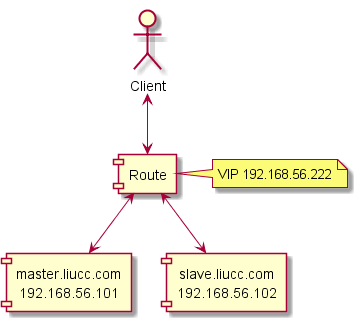
\includegraphics[width=0.5\textwidth]{img/heartbeat.png}
  \caption{heartbeat实验拓扑}
\end{figure}

映射服务所用的IP地址需要一直能够访问得到。通常,Heartbeat会为你将指定
的IP地址分配给主服务器上的虚拟网络接口卡。如果主服务器出现了故障,集群
会自动将IP地址切换到另一台可用服务器上的虚拟网卡。如果主服务器恢复正常
运行,它会再次将IP地址切换回到主服务器。由于具有迁移属性,这个IP地址被
称为“浮动”地址。

\section{安装Heartbeat}

在所有服务器上安装软件包

想组建集群,首先要使用yum,在每一个节点上安装必要的软件包:

\begin{verbatim}
yum install PyXML cluster-glue cluster-glue-libs resource-agents
\end{verbatim}

下一步,下载和安装官方CentOS软件库里面没有的两个Heartbeat RPM文件。

另外,你可以将EPEL软件库添加到源文件,并使用yum进行安装。

Heartbeat会管理Apache的httpd服务的开启和停止,所以停止Apache,并禁止它自动开启:

\begin{verbatim}
service httpd stop
chkconfig httpd off
\end{verbatim}

设置主机名称

现在设置服务器的主机名称,为此编辑每个系统上的/etc/sysconfig/network,并更改HOSTNAME这一行:

HOSTNAME=xxxxx.liucc.com 新的主机名称会在服务器下一次启动时激活。
你可以使用hostname命令立即激活它,不需要重启服务器:

hostname xxxxx.liucc.com 你可以在每一台服务器上运行uname -n,以此证实主机名称已正确设置好。

\section{配置Heartbeat}

想配置Heartbeat,首先要将其默认配置文件从/usr拷贝到/etc/ha.d/:

\begin{verbatim}
cp /usr/share/doc/heartbeat-3.0.4/authkeys /etc/ha.d/
cp /usr/share/doc/heartbeat-3.0.4/ha.cf /etc/ha.d/
cp /usr/share/doc/heartbeat-3.0.4/haresources /etc/ha.d/
\end{verbatim}

然后,你还得改动全部集群节点上的所有三个文件,以便与你的需求相匹配。

authkeys文件含有集群节点彼此联系时所使用的预共享密码。集群里面的每个
Heartbeat消息都含有该密码,节点只处理拥有正确密码的那些消息。Heartbeat
支持SHA1密码和MD5密码。在authkeys文件中,下列指令将验证方法设置为SHA1,
并且定义了所使用的密码:

\begin{verbatim}
auth 2
2 sha1 pre-shared-password
\end{verbatim}

保存该文件,然后使用命令

\begin{verbatim}
chmod 600 /etc/ha.d/authkeys
\end{verbatim}

为该文件授予只有root用户可以读写的权限。

下一步,在ha.cf文件中,定义计时器、集群节点、消息传递机制、第4层端口及其他设置:

\begin{verbatim}
## 日志##
logfile /var/log/ha-log
logfacility local0hea
## 计时器##
## 所有计时器设成以秒为单位。如果你需要以毫秒为单位设置时间,就使用‘ms’。##
## heartbeat间隔时间##
keepalive 2

## 超过这个时间后,节点被认为已停滞##
deadtime 15
## 一些服务器花更长的时间来启动。该计时器定义了证实服务器宕机之前所等待的额外时间。##
## 该计时器的建议时间是停滞计时器的至少一倍。##
initdead 120
## 消息传递参数##
udpport 694
bcast eth0
## 你还可以使用多播或单播##
## 节点定义##
## 确保主机名称符合uname -n ##
node master.liucc.com
node slave.liucc.com
\end{verbatim}

最后,文件haresources含有Heartbeat认为是主节点的那台服务器的主机名称,
另外还含有浮动IP地址。该文件在所有服务器上都一模一样,这点很重要。只要
主节点在正常运行,它就服务所有请求;Heartbeat停止其他所有节点上的高可
用性服务。Heartbeat检测到该主节点停机运行后,它会在集群中的下一个可用
节点上自动开启服务。主节点恢复正常运行后,Heartbeat会让它再次接手任务,
服务所有请求。最后,该文件含有负责高可用性服务的脚本的名称:这里是
httpd。其他可能出现的值有squid、smb、nmb或postfix,映射到通常位于
/etc/init.d/目录中的服务启动脚本的名称。

在haresources中,定义master.liucc.com.com为主服务器,定义
192.168.56.222为浮动IP地址,定义 httpd为高可用性服务。你不需要创建任何
接口,也不需要为任何接口手动分配浮动IP地址,Heartbeat为我们处理这项任
务:

\begin{verbatim}
master.liucc.com 192.168.56.222 httpd
\end{verbatim}

每一台服务器上的配置文件准备就绪后,开启Heartbeat服务,并将它添加到系
统启动项:

\begin{verbatim}
service heartebeat start
chkconfig heartbeat on
\end{verbatim}

这时,可以查看一下master节点上的IP地址信息,

\begin{verbatim}
[root@master ~]# ifconfig 
eth0      Link encap:Ethernet  HWaddr 08:00:27:4D:65:37  
          inet addr:192.168.56.101  Bcast:192.168.56.255  Mask:255.255.255.0
          inet6 addr: fe80::a00:27ff:fe4d:6537/64 Scope:Link
          UP BROADCAST RUNNING MULTICAST  MTU:1500  Metric:1
          RX packets:13825 errors:0 dropped:0 overruns:0 frame:0
          TX packets:10376 errors:0 dropped:0 overruns:0 carrier:0
          collisions:0 txqueuelen:1000 
          RX bytes:3095677 (2.9 MiB)  TX bytes:2253820 (2.1 MiB)

eth0:0    Link encap:Ethernet  HWaddr 08:00:27:4D:65:37  
          inet addr:192.168.56.222  Bcast:192.168.56.255  Mask:255.255.255.0
          UP BROADCAST RUNNING MULTICAST  MTU:1500  Metric:1

eth1      Link encap:Ethernet  HWaddr 08:00:27:BC:A6:E2  
          inet addr:192.168.56.201  Bcast:192.168.56.255  Mask:255.255.255.0
          inet6 addr: fe80::a00:27ff:febc:a6e2/64 Scope:Link
          UP BROADCAST RUNNING MULTICAST  MTU:1500  Metric:1
          RX packets:21609 errors:0 dropped:0 overruns:0 frame:0
          TX packets:61 errors:0 dropped:0 overruns:0 carrier:0
          collisions:0 txqueuelen:1000 
          RX bytes:4926438 (4.6 MiB)  TX bytes:6922 (6.7 KiB)

lo        Link encap:Local Loopback  
          inet addr:127.0.0.1  Mask:255.0.0.0
          inet6 addr: ::1/128 Scope:Host
          UP LOOPBACK RUNNING  MTU:16436  Metric:1
          RX packets:2696 errors:0 dropped:0 overruns:0 frame:0
          TX packets:2696 errors:0 dropped:0 overruns:0 carrier:0
          collisions:0 txqueuelen:0 
          RX bytes:5452373 (5.1 MiB)  TX bytes:5452373 (5.1 MiB)
\end{verbatim}

你可以借助命令tailf /var/log/ha-log,密切关注Heartbeat日志。

Heartbeat可用于多项服务。比如说,haresources中的下列指令将让Heartbeat
同时管理Apache服务和Samba服务:

master.liucc.com 192.168.56.222 httpd smb nmb 不过,除非你还在运行
Pacemaker之类的集群资源管理器(CRM),否则我不建议使用Heartbeat在单一
集群中提供多项服务。要是没有Pacemaker,Heartbeat使用IP地址监测第3层中
的集群节点。只要IP地址可以访问得到,Heartbeat无视服务在服务器节点上可
能遇到的任何崩溃或困难。

\section{测试}

一旦Heartbeat设置并运行起来,不妨对它测试一下。在所有三台服务器上创建
单独的index.html文件,那样你就能看清哪台服务器在服务页面。浏览到
192.168.56.222,如果你设置好了DNS,也可以浏览到相应域名。页面应该会从
master.liucc.com.com加载,你可以查看服务器1中的Apache日志文件来核实这一
点。试着刷新页面,证实该页面是否每次都从同一台服务器加载。

关闭主节点后,主节点产生的日志信息,

\begin{verbatim}
Apr 14 11:43:48 master.liucc.com heartbeat: [13928]: info: Heartbeat shutdown in progress. (13928)
Apr 14 11:43:48 master.liucc.com heartbeat: [14300]: info: Giving up all HA resources.
ResourceManager[14313]:	2015/04/14_11:43:48 info: Releasing resource group: master.liucc.com 192.168.56.222 httpd
ResourceManager[14313]:	2015/04/14_11:43:48 info: Running /etc/init.d/httpd  stop
ResourceManager[14313]:	2015/04/14_11:43:48 info: Running /etc/ha.d/resource.d/IPaddr 192.168.56.222 stop
IPaddr[14386]:	2015/04/14_11:43:48 INFO: ifconfig eth0:0 down
IPaddr[14372]:	2015/04/14_11:43:48 INFO:  Success
Apr 14 11:43:48 master.liucc.com heartbeat: [14300]: info: All HA resources relinquished.
Apr 14 11:43:49 master.liucc.com heartbeat: [13928]: WARN: 1 lost packet(s) for [slave.liucc.com] [36:38]
Apr 14 11:43:49 master.liucc.com heartbeat: [13928]: info: No pkts missing from slave.liucc.com!
Apr 14 11:43:50 master.liucc.com heartbeat: [13928]: info: killing HBFIFO process 13930 with signal 15
Apr 14 11:43:50 master.liucc.com heartbeat: [13928]: info: killing HBWRITE process 13931 with signal 15
Apr 14 11:43:50 master.liucc.com heartbeat: [13928]: info: killing HBREAD process 13932 with signal 15
Apr 14 11:43:50 master.liucc.com heartbeat: [13928]: info: Core process 13932 exited. 3 remaining
Apr 14 11:43:50 master.liucc.com heartbeat: [13928]: info: Core process 13931 exited. 2 remaining
Apr 14 11:43:50 master.liucc.com heartbeat: [13928]: info: Core process 13930 exited. 1 remaining
Apr 14 11:43:50 master.liucc.com heartbeat: [13928]: info: master.liucc.com Heartbeat shutdown complete.
\end{verbatim}

此时,备节点上的日志信息为:

\begin{verbatim}
ResourceManager[13103]:	2015/04/14_11:43:49 info: Acquiring resource group: master.liucc.com 192.168.56.222 httpd
IPaddr[13131]:	2015/04/14_11:43:49 INFO:  Resource is stopped
ResourceManager[13103]:	2015/04/14_11:43:49 info: Running /etc/ha.d/resource.d/IPaddr 192.168.56.222 start
IPaddr[13194]:	2015/04/14_11:43:49 INFO: Using calculated nic for 192.168.56.222: eth0
IPaddr[13194]:	2015/04/14_11:43:49 INFO: Using calculated netmask for 192.168.56.222: 255.255.255.0
IPaddr[13194]:	2015/04/14_11:43:49 INFO: eval ifconfig eth0:0 192.168.56.222 netmask 255.255.255.0 broadcast 192.168.56.255
IPaddr[13180]:	2015/04/14_11:43:49 INFO:  Success
ResourceManager[13103]:	2015/04/14_11:43:49 info: Running /etc/init.d/httpd  start
mach_down[13076]:	2015/04/14_11:43:49 info: /usr/share/heartbeat/mach_down: nice_failback: foreign resources acquired
mach_down[13076]:	2015/04/14_11:43:49 info: mach_down takeover complete for node master.liucc.com.
Apr 14 11:43:49 slave.liucc.com heartbeat: [12969]: info: mach_down takeover complete.
Apr 14 11:44:05 slave.liucc.com heartbeat: [12969]: WARN: node master.liucc.com: is dead
Apr 14 11:44:05 slave.liucc.com heartbeat: [12969]: info: Dead node master.liucc.com gave up resources.
Apr 14 11:44:05 slave.liucc.com heartbeat: [12969]: info: Link master.liucc.com:eth0 dead.
\end{verbatim}

如果这一切进展良好,测试一下故障切换机制:停止master.liucc.com上的
Heartbeat服务。浮动IP地址应该会迁移到服务器slave上,页面应该会从该服务
器加载。迅速看一下slave的Apache日志,应该可以证实这一点。如果我们重启
了服务器master上的heartbeat服务,浮动IP地址应该会按照haresources中的设
置,从活动节点迁移到服务器slave上。

当我们把master上的heartbeart重新运行起来,这时,观察slave节点的日志信息,

\begin{verbatim}
ResourceManager[13654]:	2015/04/14_13:52:20 info: Releasing resource group: master.liucc.com 192.168.56.222 httpd
ResourceManager[13654]:	2015/04/14_13:52:20 info: Running /etc/init.d/httpd  stop
ResourceManager[13654]:	2015/04/14_13:52:21 info: Running /etc/ha.d/resource.d/IPaddr 192.168.56.222 stop
IPaddr[13727]:	2015/04/14_13:52:21 INFO: ifconfig eth0:0 down
IPaddr[13713]:	2015/04/14_13:52:21 INFO:  Success
Apr 14 13:52:21 slave.liucc.com heartbeat: [13641]: info: foreign HA resource release completed (standby).
Apr 14 13:52:21 slave.liucc.com heartbeat: [12969]: info: Local standby process completed [foreign].
Apr 14 13:52:21 slave.liucc.com heartbeat: [12969]: WARN: 1 lost packet(s) for [master.liucc.com] [10:12]
Apr 14 13:52:21 slave.liucc.com heartbeat: [12969]: info: remote resource transition completed.
Apr 14 13:52:21 slave.liucc.com heartbeat: [12969]: info: No pkts missing from master.liucc.com!
Apr 14 13:52:21 slave.liucc.com heartbeat: [12969]: info: Other node completed standby takeover of foreign resources.
\end{verbatim}

正如我们所见,使用Heartbeat,在RHEL下组建一个高可用性的Apache集群是件
很容易的事。虽然我们使用了2台服务器,但Heartbeat在节点数量更多或更少
的环境下应该同样没问题。Heartbeat对节点数量没有任何限制,所以你可以根
据需要扩展所设置环境的规模。



\chapter{Nginx负载均衡与高可用集群}
\label{chap:nginxLB}

Nginx的负载均衡功能依赖于\verb|ngx_upstream_module|模块,所支持的代理方
式有,

\begin{enumerate}[itemsep=0pt,parsep=0pt]
\item proxy\_pass
\item fastcgi\_pass
\item memcached\_pass
\end{enumerate}

\section{upstream模块介绍}
\label{sec:upstreamIntro}



\section{Nginx负载均衡方法介绍}

\section{准备工作}
\label{sec:nginxPrepare}

\section{Nginx+KeepAlived高可用}
\label{sec:NginxAndKeepalived}

Nginx负载均衡器总会存在单点故障的问题,所以,有必要对Nginx负载均衡器进
行高可用配置。


\chapter{Pacemaker+Corosync高可用集群}

高可用集群,是指以减少服务中断时间为目的的服务器集群技术。高可用集群的
出现是为了减少由计算机硬件和软件易错性所带来的损失。它通过保护用户的业
务程序对外不间断提供的服务,把因软件/硬件/人为造成的故障对业务的影响降
低到最小程度。如果某个节点失效,它的备援节点将在数秒钟的时间内接管它的
职责。因此,对于用户而言,集群永远不会停机。高可用集群软件的主要作用就
是实现故障检查和业务切换的自动化。

下面案例是httpd服务的具体实现:

\section{准备工作}

本案例的拓扑图为:

\begin{figure}[!htbp]
  \centering
  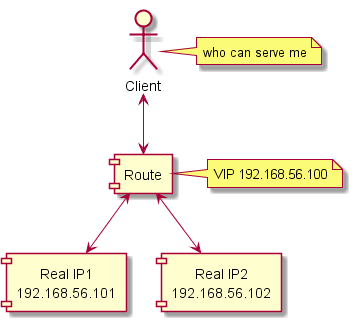
\includegraphics[width=0.5\textwidth]{img/web_topo.png}
  \caption{corosync实验拓扑}
\end{figure}

为了配置一台主机成为HA的节点,通常需要做出如下的准备工作:
\begin{enumerate}[itemsep=0pt,parsep=0pt]
  \item 所有节点的主机名和对应的IP地址解析服务可以正常工作,且每个节点
    的主机名称需要跟“uname -n”命令的结果保持一致;因此,需要保证两个节
    点上的/etc/hosts文件一致;
  \item 两个节点可以基于密钥进行ssh通信;
\end{enumerate}

具体实现为:

\begin{verbatim}
[root@master ~]# cat /etc/hosts
192.168.56.101   master.liucc.com master
192.168.56.102	 slave.liucc.com slave
\end{verbatim}

为了使得重新启动系统后仍能保持如上的主机名称,还需要分别在各节点修改
/etc/sysconfig/network文件。

\begin{verbatim}
master:
# sed -i 's@\(HOSTNAME=\).*@\1master.liucc.com@g'  /etc/sysconfig/network
# hostname master.liucc.com

slave:
# sed -i 's@\(HOSTNAME=\).*@\1slave.liucc.com@g' /etc/sysconfig/network
# hostname slave.liucc.com
\end{verbatim}

各节点生成ssh密钥:

\begin{verbatim}
master:
# cd /root/.ssh
# ssh-keygen -t rsa
# scp id_rsa.pub slave:/root/.ssh/authorized_keys

slave:
# cd /root/.ssh
# ssh-keygen -t rsa
# cat id_rsa.pub >> authorized_keys
# scp authorized_keys master:/root/.ssh
\end{verbatim}

\section{安装软件包}

首先确保已配置本地yum源,然后安装如下依赖包:

\begin{verbatim}
[root@master ~] # yum -y install libibverbs librdmacm lm_sensors \
> libtool-ltdl openhpi-libs openhpi perl-TimeDate
\end{verbatim}

安装完毕依赖包,接下来安装corosync及pacemaker,这里已经准备了相应的软件包,

\begin{verbatim}
[root@master ~]# ls clusterlab
cluster-glue-1.0.6-1.6.el5.i386.rpm       
cluster-glue-libs-1.0.6-1.6.el5.i386.rpm  
corosync-1.2.7-1.1.el5.i386.rpm           
corosynclib-1.2.7-1.1.el5.i386.rpm        
heartbeat-3.0.3-2.3.el5.i386.rpm          
heartbeat-libs-3.0.3-2.3.el5.i386.rpm
libesmtp-1.0.4-5.el5.i386.rpm
pacemaker-1.1.5-1.1.el5.i386.rpm
pacemaker-libs-1.1.5-1.1.el5.i386.rpm
resource-agents-1.0.4-1.1.el5.i386.rpm

[root@master ~]# cd clusterlab
[root@master clusterlab]# yum -y --nogpgcheck localinstall *.rpm
Total size: 17 M
Downloading Packages:
Running rpm_check_debug
Running Transaction Test
Finished Transaction Test
Transaction Test Succeeded
Running Transaction
  Installing     : libesmtp
  Installing     : cluster-glue-libs
  Installing     : corosynclib
  Installing     : cluster-glue
  Installing     : resource-agents 
  Installing     : corosync
  Installing     : heartbeat-libs
  Installing     : pacemaker
  Installing     : pacemaker-libs 
  Installing     : heartbeat
Installed products updated.

Complete!
\end{verbatim}

\section{配置及启动corosync}

下面的配置在master上完成,编辑/etc/corosync/corosync.conf

\begin{verbatim}
[root@master ~]# cd /etc/corosync
[root@master corosync]# cp corosync.conf.example corosync.conf
\end{verbatim}

在文件尾部添加如下内容:

\begin{verbatim}
[root@master corosync]# tail corosync.conf
service {
  ver:  0
  name: pacemaker
}

aisexec {
  user: root
  group:  root
}
\end{verbatim}

并设定此配置文件中 bindnetaddr后面的IP地址为你的网卡所在网络的网络地址,
我们这里的两个节点在192.168.56.0网络,因此这里将其设定为192.168.56.0。
整个配置文件如下:

\begin{verbatim}
[root@master corosync]# cat corosync.conf
# Please read the corosync.conf.5 manual page
compatibility: whitetank

totem {
        version: 2 #版本号
        secauth: off #安全认证
        threads: 0 #线程数,根据CPU个数和核心数确定
        interface {
	        ringnumber: 0 #冗余环号,节点有多个网卡是可定义对应网卡在一个环内
	        bindnetaddr: 192.168.56.0 # 绑定网络地址
	        mcastaddr: 226.94.1.1     # 心跳信息所使用的组播地址
	        mcastport: 5405           # 心跳组播使用的端口
        }
}

logging {
        fileline: off #指定要打印的行
        to_stderr: no #是否发送到标准错误输出
        to_logfile: yes #记录到文件
        to_syslog: yes #记录到syslog
        logfile: /var/log/cluster/corosync.log # corosync日志文件
        debug: off
        timestamp: on #是否打印时间戳,利于定位错误(会消耗CPU资源)
        logger_subsys {
	        subsys: AMF
	        debug: off
        }
}

amf {
        mode: disabled
}

service {
        ver: 0
        name: pacemaker # 定义corosync在启动时自动启动pacemaker
}

aisexec {               # 表示启动corosync的ais功能,以哪个用户身份运行
        user: root
        group: root
}
\end{verbatim}

生成节点间通信时用到的认证密钥文件:

\begin{verbatim}
[root@master corosync]# corosync-keygen
[root@master corosync]# scp -p corosync.conf authkey slave:/etc/corosync

建立corosync日志所需要的目录
[root@master corosync]# mkdir /var/log/cluster
[root@master corosync]# ssh slave "mkdir /var/log/cluster"
\end{verbatim}

接下来就可以启动corosync了,

\begin{verbatim}
[root@master ~]# /etc/init.d/corosync start
Starting Corosync Cluster Engine (corosync):               [  OK  ]
\end{verbatim}

此时,可以查看一下关于corosync引擎是否正常启动的系统日志,

\begin{verbatim}
[root@master corosync]# grep -e "Corosync Cluster Engine" -e "configuration file" /var/log/messages
Feb 28 11:17:02 unionpay smartd[2787]: Opened configuration file /etc/smartd.conf 
Feb 28 11:21:24 master smartd[2770]: Opened configuration file /etc/smartd.conf 
Feb 28 11:44:06 master smartd[2766]: Opened configuration file /etc/smartd.conf 
Feb 28 13:43:05 master corosync[7859]:   [MAIN  ] Corosync Cluster Engine ('1.2.7'): started and ready to provide service.
Feb 28 13:43:05 master corosync[7859]:   [MAIN  ] Successfully read main configuration file '/etc/corosync/corosync.conf'.
\end{verbatim}

查看初始化成员节点通知是否正常发出,
\begin{verbatim}
[root@master corosync]# grep TOTEM /var/log/messages
Feb 28 13:43:05 master corosync[7859]:   [TOTEM ] Initializing transport (UDP/IP).
Feb 28 13:43:05 master corosync[7859]:   [TOTEM ] Initializing transmit/receive security: libtomcrypt SOBER128/SHA1HMAC (mode 0).
Feb 28 13:43:05 master corosync[7859]:   [TOTEM ] The network interface [192.168.56.101] is now up.
Feb 28 13:43:05 master corosync[7859]:   [TOTEM ] A processor joined or left the membership and a new membership was formed.
\end{verbatim}

检查启动过程中是否有错误产生:
\begin{verbatim}
# grep ERROR: /var/log/messages | grep -v unpack_resources
\end{verbatim}

查看pacemaker是否正常启动:
\begin{verbatim}
[root@master corosync]#  grep pcmk_startup /var/log/messages
Feb 28 13:43:05 master corosync[7859]:   [pcmk  ] info: pcmk_startup: CRM: Initialized
Feb 28 13:43:05 master corosync[7859]:   [pcmk  ] Logging: Initialized pcmk_startup
Feb 28 13:43:05 master corosync[7859]:   [pcmk  ] info: pcmk_startup: Maximum core file size is: 4294967295
Feb 28 13:43:05 master corosync[7859]:   [pcmk  ] info: pcmk_startup: Service: 9
Feb 28 13:43:05 master corosync[7859]:   [pcmk  ] info: pcmk_startup: Local hostname: master.liucc.com
\end{verbatim}

如果上面命令执行均没有问题,接着可以执行如下命令启动node2上的corosync
\begin{verbatim}
[root@slave cluster]# ssh slave -- /etc/init.d/corosync start
The authenticity of host 'slave (192.168.56.102)' can't be established.
RSA key fingerprint is 3e:36:02:7a:4c:3c:0d:39:d0:51:a4:86:0f:85:97:c8.
Are you sure you want to continue connecting (yes/no)? yes
Warning: Permanently added 'slave' (RSA) to the list of known hosts.
Starting Corosync Cluster Engine (corosync): [  OK  ]
[root@slave cluster]# ssh slave -- /etc/init.d/corosync status
corosync (pid  10867) is running...
\end{verbatim}

注意:启动node2需要在node1上使用如上命令进行,不要在node2节点上直接启动;

使用如下命令查看集群节点的启动状态:
\begin{verbatim}
[root@master corosync]# crm status
============
Last updated: Sat Feb 28 13:48:11 2015
Stack: openais
Current DC: master.liucc.com - partition with quorum
Version: 1.1.5-1.1.el5-01e86afaaa6d4a8c4836f68df80ababd6ca3902f
2 Nodes configured, 2 expected votes
0 Resources configured.
============

Online: [ master.liucc.com slave.liucc.com ]

\end{verbatim}

从上面的信息可以看出两个节点都已经正常启动,并且集群已经处于正常工作状
态。

由于corosync默认启用了stonith,而当前集群并没有相应的stonith设备,因此
此默认配置目前尚不可用,这可以通过如下命令验正:

\begin{verbatim}
[root@master corosync]# crm_verify -L
crm_verify[7926]: 2015/02/28_13:51:01 ERROR: unpack_resources: Resource start-up disabled since no STONITH resources have been defined
crm_verify[7926]: 2015/02/28_13:51:01 ERROR: unpack_resources: Either configure some or disable STONITH with the stonith-enabled option
crm_verify[7926]: 2015/02/28_13:51:01 ERROR: unpack_resources: NOTE: Clusters with shared data need STONITH to ensure data integrity
Errors found during check: config not valid
  -V may provide more details

\end{verbatim}

我们里可以通过如下命令先禁用stonith:

\begin{verbatim}
[root@master corosync]# crm configure property stonith-enabled=false
\end{verbatim}

使用如下命令查看当前的配置信息:

\begin{verbatim}
[root@master corosync]# crm configure show
node master.liucc.com
node slave.liucc.com
property $id="cib-bootstrap-options" \
	dc-version="1.1.5-1.1.el5-01e86afaaa6d4a8c4836f68df80ababd6ca3902f" \
	cluster-infrastructure="openais" \
	expected-quorum-votes="2" \
	stonith-enabled="false"
\end{verbatim}

从中可以看出stonith已经被禁用。上面的crm,crm\_verify命令是1.0后的版本的
pacemaker提供的基于命令行的集群管理工具;可以在集群中的任何一个节点上执
行。

\section{为集群添加资源}

corosync支持heartbeat,LSB和ocf等类型的资源代理,目前较为常用的类型为
LSB和OCF两类,stonith类专为配置stonith设备而用;可以通过如下命令查看当
前集群系统所支持的类型:

\begin{verbatim}
# crm ra classes 
heartbeat
lsb
ocf / heartbeat pacemaker
stonith
\end{verbatim}

如果想要查看某种类别下的所用资源代理的列表,可以使用类似如下命令实现:

\begin{verbatim}
[root@master ~]# crm ra list lsb
NetworkManager      acpid               anacron             apmd                atd                 auditd              autofs
avahi-daemon        avahi-dnsconfd      bluetooth           capi                conman              corosync            cpuspeed
crond               cups                cups-config-daemon  dnsmasq             dund                firstboot           functions
gpm                 haldaemon           halt                heartbeat           hidd                hplip               httpd
ip6tables           ipmi                iptables            irda                irqbalance          iscsi               iscsid
isdn                kdump               killall             krb524              kudzu               lm_sensors          logd
lvm2-monitor        mcstrans            mdmonitor           mdmpd               messagebus          microcode_ctl       multipathd
mysqld              netconsole          netfs               netplugd            network             nfs                 nfslock
nscd                ntpd                openhpid            openibd             pacemaker           pand                pcscd
portmap             postgresql-9.0      psacct              rawdevices          rdisc               readahead_early     readahead_later
restorecond         rhnsd               rhsmcertd           rpcgssd             rpcidmapd           rpcsvcgssd          saslauthd
sendmail            setroubleshoot      single              smartd              snmpd               snmptrapd           sshd
syslog              sysstat             tomcat              vboxadd             vboxadd-service     vboxadd-x11         vncserver
vsftpd              wdaemon             winbind             wpa_supplicant      xfs                 xinetd              ypbind
yum-updatesd

[root@master ~]# crm ra list ocf heartbeat
AoEtarget           AudibleAlarm        CTDB                ClusterMon          Delay               Dummy               EvmsSCC
Evmsd               Filesystem          ICP                 IPaddr              IPaddr2             IPsrcaddr           IPv6addr
LVM                 LinuxSCSI           MailTo              ManageRAID          ManageVE            Pure-FTPd           Raid1
Route               SAPDatabase         SAPInstance         SendArp             ServeRAID           SphinxSearchDaemon  Squid
Stateful            SysInfo             VIPArip             VirtualDomain       WAS                 WAS6                WinPopup
Xen                 Xinetd              anything            apache              conntrackd          db2                 drbd
eDir88              exportfs            fio                 iSCSILogicalUnit    iSCSITarget         ids                 iscsi
jboss               ldirectord          mysql               mysql-proxy         nfsserver           nginx               oracle
oralsnr             pgsql               pingd               portblock           postfix             proftpd             rsyncd
scsi2reservation    sfex                syslog-ng           tomcat              vmware 

[root@master ~]# crm ra list ocf pacemaker
ClusterMon    Dummy         HealthCPU     HealthSMART   Stateful      SysInfo       SystemHealth  controld      o2cb          ping
pingd      

[root@master ~]# crm ra list stonith
apcmaster               apcmastersnmp           apcsmart                baytech                 bladehpi                cyclades
external/drac5          external/dracmc-telnet  external/hmchttp        external/ibmrsa         external/ibmrsa-telnet  external/ipmi
external/ippower9258    external/kdumpcheck     external/rackpdu        external/riloe          external/sbd            external/vmware
external/xen0           external/xen0-ha        fence_legacy            ibmhmc                  ipmilan                 meatware
nw_rpc100s              rcd_serial              rps10                   suicide                 wti_mpc                 wti_nps
\end{verbatim}

\begin{verbatim}
# crm ra info [class:[provider:]]resource_agent
例如:
[root@master ~]# crm ra info ocf:heartbeat:IPaddr
Manages virtual IPv4 addresses (portable version) (ocf:heartbeat:IPaddr)

This script manages IP alias IP addresses
It can add an IP alias, or remove one.

Parameters (* denotes required, [] the default):

ip* (string): IPv4 address
    The IPv4 address to be configured in dotted quad notation, for example
    "192.168.1.1".

nic (string, [eth0]): Network interface
    The base network interface on which the IP address will be brought
    online.
    
    If left empty, the script will try and determine this from the
    routing table.
    
    Do NOT specify an alias interface in the form eth0:1 or anything here;
    rather, specify the base interface only.
    
    Prerequisite:
    
    There must be at least one static IP address, which is not managed by
    the cluster, assigned to the network interface.
    
    If you can not assign any static IP address on the interface,
    modify this kernel parameter:
    sysctl -w net.ipv4.conf.all.promote_secondaries=1
    (or per device)

cidr_netmask (string): Netmask
    The netmask for the interface in CIDR format. (ie, 24), or in
    dotted quad notation  255.255.255.0).
    
    If unspecified, the script will also try to determine this from the
    routing table.

broadcast (string): Broadcast address
    Broadcast address associated with the IP. If left empty, the script will
    determine this from the netmask.

iflabel (string): Interface label
    You can specify an additional label for your IP address here.

lvs_support (boolean, [false]): Enable support for LVS DR
    Enable support for LVS Direct Routing configurations. In case a IP
    address is stopped, only move it to the loopback device to allow the
    local node to continue to service requests, but no longer advertise it
    on the network.

local_stop_script (string): 
    Script called when the IP is released

local_start_script (string): 
    Script called when the IP is added

ARP_INTERVAL_MS (integer, [500]): milliseconds between gratuitous ARPs
    milliseconds between ARPs

ARP_REPEAT (integer, [10]): repeat count
    How many gratuitous ARPs to send out when bringing up a new address

ARP_BACKGROUND (boolean, [yes]): run in background
    run in background (no longer any reason to do this)

ARP_NETMASK (string, [ffffffffffff]): netmask for ARP
    netmask for ARP - in nonstandard hexadecimal format.

Operations' defaults (advisory minimum):

    start         timeout=20s
    stop          timeout=20s
    monitor       interval=5s timeout=20s
\end{verbatim}

\section{为Web创建IP资源}

接下来要创建的web集群创建一个IP地址资源,以在通过集群提供web服务时使用;
这可以通过如下方式实现:

语法:

\begin{verbatim}
primitive <rsc> [<class>:[<provider>:]]<type>
          [params attr_list]
          [operations id_spec]
            [op op_type [<attribute>=<value>...] ...]

op_type :: start | stop | monitor
\end{verbatim}

例子:

\begin{verbatim}
 primitive apcfence stonith:apcsmart \
          params ttydev=/dev/ttyS0 hostlist="node1 node2" \
          op start timeout=60s \
          op monitor interval=30m timeout=60s
\end{verbatim}


\section{高可用验证}

\chapter{DRBD}
\label{chap:drbd}

distributed replicated block device

a software-based, shared-nothing, replicated storage solution
mirroring the content of block devices (hard disks, partitions,
logical volumes etc.) between servers.

DRBD's core functionality is implemented by way of a Linux Kernel
module.

User space administration tools

drbdadm

The high-level administration tool of the DRBD program suite. It
obtains all DRBD configuration parameters from the configuration 
file /etc/drbd.conf

drbdsetup

The program that allows users to configure the DRBD module that has
been loaded into the running kernel. It is the low-level tool within
the DRBD program suite.

Resource roles

In DRBD, every resource has a role, which may be Primary or Secondary.

Primary

A DRBD device in the primary role can be used unrestrictedly for read
and write operations. It may be used for creating and mounting file
systems, raw or direct I/O to the block device, etc.

Secondary

A DRBD device in the secondary role receives all updates from the perr
node's device, but otherwise disallows access completely.  It can not
be used by applications, neither for read nor write access.

DRBD modes

Single-primary mode
\begin{quote}
Any resource is, at any given time, in the primary role on only one
cluster member.

Only one cluster node manipulates the data at any moment.

This mode can be used with any conventional file system (ext3, ext4,
XFS, etc.)

Deploying DRBD in single-primary mode is the canonical approach for
high availability (fail-over capable) clusters.
\end{quote}

Dual-primary mode
\begin{quote}
Any resource is, at any given time, in the primary role on both
cluster nodes.

Since concurrent access to the data is thus possible, this mode
requires the use of a shared cluster file system that utilizes a
distributed lock manager. Examples include GFS and OCFS2.

Deploying DRBD in dual-primary mode is the preferred approach for
load-balancing clusters which require concurrent data access from two
nodes.

Disabled by default, and must be enabled explicitly in DRBD's
configuration file.

Available in DRBD 8.0 and later.
\end{quote}
 
\section{三种同步模式}

\begin{enumerate}[itemsep=0pt,parsep=0pt]
\item 协议A
\begin{quote}
异步复制协议。只要主节点完成本地写操作就认为写操作完成,并且需要复制的
数据包会被存储到本地TCP发送缓冲中。当发生failover故障,数据可能会丢失。
当发生failover故障时,在备节点的数据被认为仍是稳固的,然而,在crash发生
的时间点上很多最新的更新操作会丢失。
\end{quote}

\item 协议B
\begin{quote}
内存同步(半同步)复制协议。当本地盘的写已经完成,并且复制数据包已经到
达对应从节点,此时主节点才认为磁盘写已经完成。通常情况下,发生failover
不会导致数据丢失(因为后备系统内存中已经获得了数据更新)。然而,如果所
有节点同时出现电源故障,则主节点数据存储会产生不可逆的错误结构,主节点
上多数最新写入的数据可能会丢失。
\end{quote}

\item 协议C
\begin{quote}
同步复制协议。只有在本地和远程磁盘都确定写入已经完成时,主节点才会认为
写入完成。这样可确保发生故障时不会导致任何数据丢失。如果发生数据丢失的
现象,那也只会在所有节点同时存在错误存储时才会发生。
\end{quote}
\end{enumerate}

Efficient synchronization
\begin{quote}
Synchronization is necessary if the replication link has been
interrupted for any reason

1. failure of the primary node
2. failure of the secondary node
3. or interruption of the replication link

(Re-)synchronization is distinct from device replication
\end{quote}

Split brain
\begin{quote}
Split brain is a situation where, due to temporary failure of all
network links between cluster nodes, and possibly due to intervension
by a cluster management software or human error, both nodes switched
to the primary role while disconnected.
\end{quote}

automatic recovery
\begin{quote}
DRBD allows for automatic operator notification (by email or other
means) when it detects split brain.

DRBD has several resolution algorithms available for resolving the
split brain automaticly.

1. Discarding modifications made on the "younger" primary
2. Discarding modifications made on the "older" primary
3. Discarding modifications on the primary with fewer changes
4. Graceful recovery from split brain if one host has had no intermediate changes
\end{quote}

\section{安装及配置DRBD}

DRBD包含两大主要组件,内核空间中的驱动代码与用户空间中的管理工具。自从
Linux内核2.6.33版本及之后版本,DRBD的驱动代码已整合进了内核模块。所以,
在2.6.33版本及更新版本后,我们只需要安装用户空间的管理工具即可。否则,
我们需要同时安装内核支持模块与管理工具两个包,并且两个工具的版本号要保
持一致。

实验环境:

\begin{figure}[!h]
\centering
\begin{tabular}{llll}
\toprule
机器列表        & IP地址        & 操作系统       & DRBD版本 \\
\midrule
node1.laven.com & 192.168.1.15  & RHEL5U5 32bit  & 8.3.8 \\
node2.laven.com & 192.168.1.16  & RHEL5U5 32bit  & 8.3.8 \\
\bottomrule
\end{tabular}
\end{figure}


开始安装

\small{
\begin{verbatim}
[root@node1 ~]# ls
drbd83-8.3.8-1.el5.centos.i386.rpm
kmod-drbd83-8.3.8-1.el5.centos.i386.rpm

[root@node1 ~]# rpm -ivh kmod-drbd83-8.3.8-1.el5.centos.i386.rpm
[root@node1 ~]# rpm -ivh drbd83-8.3.8-1.el5.centos.i386.rpm
\end{verbatim}
}
\normalsize

在node2上进行同样的安装操作。

开始配置,

\small{
\begin{verbatim}
[root@node1 ~]# ls
drbd83-8.3.8-1.el5.centos.i386.rpm
kmod-drbd83-8.3.8-1.el5.centos.i386.rpm

[root@node1 ~]# rpm -ivh kmod-drbd83-8.3.8-1.el5.centos.i386.rpm
[root@node1 ~]# rpm -ivh drbd83-8.3.8-1.el5.centos.i386.rpm
\end{verbatim}
}
\normalsize

安装完成之后,来个简单的配置,使drbd可以简单的用起来。drbd的主配置文件
为/etc/drbd.conf,其中还有一个/etc/drbd.d目录,里面放置了其他的配置文件,
这也是便于管理,因此,我们可以分段进行配置,然后放置到该目录即可,在主
配置文件中使用include指令把这些文件加载进来即可。

看一下全局配置文件,

\small{
\begin{verbatim}
[root@node1 ~]# cat /etc/drbd.d/global_common.conf 
global {
   usage-count no;
   # minor-count dialog-refresh disable-ip-verification
}

common {
   protocol C;

   handlers {
      pri-on-incon-degr "/usr/lib/drbd/notify-pri-on-incon-degr.sh; \
      /usr/lib/drbd/notify-emergency-reboot.sh; \
      echo b > /proc/sysrq-trigger ; reboot -f";

      pri-lost-after-sb "/usr/lib/drbd/notify-pri-lost-after-sb.sh; \
      /usr/lib/drbd/notify-emergency-reboot.sh; \
      echo b > /proc/sysrq-trigger ; reboot -f";

      local-io-error "/usr/lib/drbd/notify-io-error.sh; \
      /usr/lib/drbd/notify-emergency-shutdown.sh; \
      echo o > /proc/sysrq-trigger ; halt -f";

      fence-peer "/usr/lib/drbd/crm-fence-peer.sh";
      split-brain "/usr/lib/drbd/notify-split-brain.sh root";
      out-of-sync "/usr/lib/drbd/notify-out-of-sync.sh root";
      before-resync-target "/usr/lib/drbd/snapshot-resync-target-lvm.sh \
      -p 15 -- -c 16k";
       after-resync-target /usr/lib/drbd/unsnapshot-resync-target-lvm.sh;
   }

   startup {
       wfc-timeout 120;
       degr-wfc-timeout 120;
   }

   disk {
       on-io-error detach;
       fencing resource-only;
   }

   net {
       cram-hmac-alg "sha1";
       shared-secret "mypass";
   }

   syncer {
       rate 100M;
   }
}
\end{verbatim}
}
\normalsize

现在定一个简单的资源r0,资源文件后缀以res结尾。

\small{
\begin{verbatim}
[root@node1 ~]# cat /etc/drbd.d/r0.res 
resource r0 {
  on node1.laven.com {
    device    /dev/drbd0;
    disk      /dev/sdb1;
    address   192.168.1.15:7789;
    meta-disk internal;
  }

  on node2.laven.com {
    device    /dev/drbd0;
    disk      /dev/sdb1;
    address   192.168.1.16:7789;
    meta-disk internal;
  }
}
\end{verbatim}
}
\normalsize

配置完毕,我们可以把这些文件复制到节点node2上去,

\small{
\begin{verbatim}
[root@node1 ~]# scp /etc/drbd.d/* node2:/etc/drbd.d/
\end{verbatim}
}
\normalsize

好了,初始化两端的drbd,然后启动drbd服务。

\small{
\begin{verbatim}
[root@node1 ~]# drbdadm create-md r0
[root@node2 ~]# drbdadm create-md r0
\end{verbatim}
}
\normalsize

初始化完毕之后,我们把node1作为主节点,node2作为从节点。之后,我们把
/dev/drbd0格式化然后挂载到/web目录下,然后在/web路下创建一些文件,然后
到node2上检查这些文件是否可以看到。

\small{
\begin{verbatim}
[root@node1 ~]# fdisk /dev/sdb -> /dev/sdb1
[root@node1 ~]# mke2fs -j /dev/drbd0
[root@node1 ~]# mount /dev/drbd0 /web
[root@node1 ~]# drbdadm primary r0
[root@node1 ~]# cd /web
[root@node1 web]# for i in {1..10}; do echo "Hello, world" > file${i}; \
> done
[root@node1 web]# ls
file1  file10  file2  file3  file4  file5  
file6  file7   file8  file9  lost+found
\end{verbatim}
}
\normalsize

这时,我们把node2作为主节点,并把/dev/drbd0挂载到/web目录下,验证是不是
有上述文件。首先,需要把/web目录umount,然后把node1变为从节点。之后,
node2需要先把自己变为主节点,然后挂载/dev/drbd0到/web下即可,

\small{
\begin{verbatim}
[root@node1 ~]# umount /web
[root@node1 ~]# drbdadm secondary r0
[root@node2 ~]# drbdadm primary r0
[root@node2 ~]# mount /dev/drbd0 /web
[root@node2 ~]# ls /web
file1  file10  file2  file3  file4  file5  
file6  file7   file8  file9  lost+found
[root@node2 ~]# cat /web/file*
Hello, world
Hello, world
Hello, world
Hello, world
Hello, world
Hello, world
Hello, world
Hello, world
Hello, world
Hello, world
\end{verbatim}
}
\normalsize

\chapter{HAproxy负载均衡与高可用}
\label{chap:haproxyCluster}

\section{关于HAproxy}
\label{sec:aboutHaproxy}

HAproxy提供高可用性、负载均衡以及基于TCP和HTTP应用的代理,支持虚拟主机,
它是免费、快速并且可靠的一种解决方案。HAproxy特别适用于那些负载特大
的web站点,这些站点通常又需要会话保持或七层处理。HAProxy运行在当前的硬
件上,完全可以支持数以万计的并发连接。并且它的运行模式使得它可以很简单
安全的整合进您当前的架构中, 同时可以保护你的web服务器不被暴露到网络
上。

HAproxy实现了一种事件驱动, 单一进程模型,此模型支持非常大的并发连接数。
多进程或多线程模型受内存限制 、系统调度器限制以及无处不在的锁限制,很少
能处理数千并发连接。事件驱动模型因为在有更好的资源和时间管理的用户空
间(User-Space) 实现所有这些任务,所以没有这些问题。此模型的弊端是,在多
核系统上,这些程序通常扩展性较差。这就是为什么他们必须进行优化以 使每
个CPU时间片(Cycle)做更多的工作。\cite{baike}

\section{环境准备}
\label{sec:envPrepareHaproxy}

\subsection{测试环境准备}

\subsection{安装EPEL源}

\section{HAproxy的高可用}
\label{sec:HighAvailableHaproxy}



\part{监控篇}

本章介绍几种监控的解决方案。

\chapter{Zabbix}

\section{Zabbix简介}

\section{Zabbix监控方案介绍}

\chapter{Prometheus}

比较流行的监控工具。

\part{自动化运维篇}

本章介绍几种自动化运维的解决方案。

% SuSE11sp2 pxe自动系统安装
\chapter{PXE批量系统安装}
\label{chap:susePXE}

\section{PXE简介}
\label{sec:introPXE}

PXE(preboot execute environment)是由Intel公司开发的最新技术,工作
于Client/Server的网络模式,支持待安装服务器(Client)通过网络从远端安装
服务器(Server)下载映像,并由此支持来自网络的操作系统的启动安装过程,
其启动安装过程中,Client端要求安装服务器动态分配IP地址,再
用TFTP(Trivial File Transfer Protocol)或MTFTP(Multicast Trivial File
Transfer Protocol)协议下载一个启动软件包到本机内存中并执行,由这个启动
软件包完成Client端的基本软件设置,从而引导安装预先安装在安装服务器上
的Client端操作系统。

\section{PXE工作原理}
\label{sec:topoPXE}

\subsection{PXE工作原理框图}
\label{sec:processPXE}

\subsection{PXE工作原理示意图}
\label{sec:processPXEInstance}

\begin{figure}[hbtp]
\centering
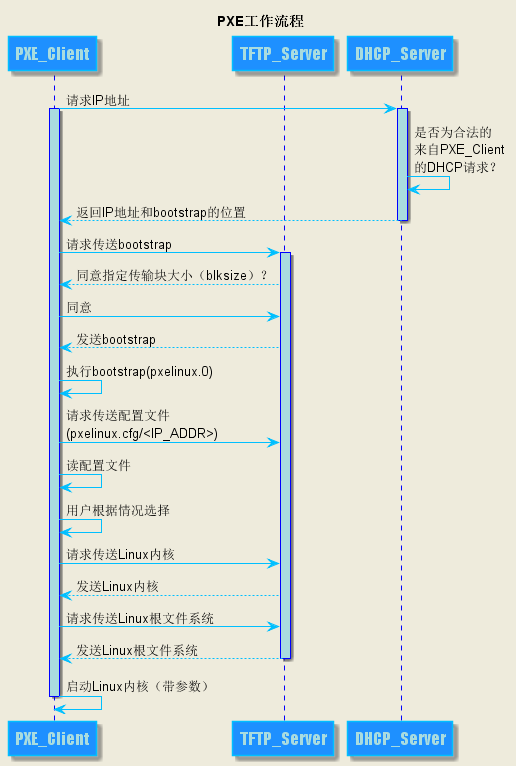
\includegraphics[width=.8\textwidth]{img/pxe01.png}
\caption{PXE工作原理示意图}
\end{figure}

工作原理示意图说明:
\begin{enumerate}[itemsep=0pt,parsep=0pt]
\item Client向PXE Server上的DHCP发送IP地址请求消息,DHCP检测Client是否
  合法(主要是检测Client的网卡MAC地址),如果合法则返回Client的IP地址,
  同时将启动文件pxelinux.0的位置信息一并传送给Client;
\item Client向PXE Server上的TFTP发送获取pxelinux.0请求消息,TFTP接收到
  消息之后再向Client发送pxelinux.0大小信息,试探Client是否满意,
  当TFTP收到Client发回的同意大小信息之后,正式向Client发送pxelinux.0;
\item Client执行接收到的pxelinux.0文件;
\item Client向TFTP发送针对本机的配置信息(记录在TFTP的pxelinux.cfg目录
  下),TFTP将配置文件发回Client,继而Client根据配置文件执行后续操作;
\item Client向TFTP发送Linux内核请求信息,TFTP接收到消息之后将内核文件发
  送给Client;
\item Client向TFTP发送根文件请求信息,TFTP接收到消息之后返回Linux根文件
  系统;
\item Client启动Linux内核(启动参数已经在4中的配置文件中设置好了);
\item Client通过NFS下载镜像文件,读取autoyast自动化安装脚本。至
  此,Client正式进入自动化安装模式开始安装系统直到完成。
\end{enumerate}

\section{开始搭建PXE服务器}
\label{sec:beginPXE}

PXE服务器包括DHCP服务、TFTP服务与NFS服务。PXE服务器安装完成后,配
置eth0的IP地址为192.168.241.1。其配置文件为:

\begin{verbatim}
# cat /etc/sysconfig/network/ifcfg-eth0
BOOTPROTO='static'
IPADDR='192.168.241.1/24'
STARTMODE='auto'
USERCONTROL='no'
\end{verbatim}

\subsection{安装及配置DHCP服务}
\label{sec:InstallDHCP}

安装DHCP服务端软件包,

\begin{verbatim}
# zypper install -y dhcp-server  
\end{verbatim}

配置DHCP服务端,修改/etc/dhcpd.conf配置文件,

\begin{verbatim}
# vi /etc/dhcpd.conf
max-lease-time 7200;
ddns-updates off;
ddns-update-style none;
default-lease-time 600;
subnet 192.168.241.0 netmask 255.255.255.0 { 
  option routers 192.168.241.254;
  next-server 192.168.241.1;
  filename "pxelinux.0";
  range 192.168.241.11 192.168.241.55;
  default-lease-time 14400;
  max-lease-time 172800;
}
host test1 {                                 
  hardware ethernet 30:30:30:30:30:30;
  fixed-address 192.168.241.11;
}  
\end{verbatim}

修改/etc/sysconfig/dhcpd配置文件,修改DHCPD\_INTERFACE的配置项,根据实
际情况修改,

\begin{verbatim}
DHCPD_INTERFACE="eth0"  
\end{verbatim}

之后,启动DHCP服务,

\begin{verbatim}
# service dhcpd start
# rcdhcpd status  
\end{verbatim}

\section{安装及配置TFTP服务}
\label{sec:InstallTFTP}

安装TFTP软件包,
\begin{verbatim}
# zypper install -y tftp  
\end{verbatim}

修改配置文件,内容如下,
\begin{verbatim}
# cat /etc/xinetd.d/tftp 
# default: off
# description: tftp service is provided primarily for booting or \
#   when a router need an upgrade. Most sites run this only on \
#   machines acting as "boot servers".
service tftp
{
        socket_type             = dgram
        protocol                = udp
        wait                    = yes
        flags                   = IPv6 IPv4
        user                    = root
        server                  = /usr/sbin/in.tftpd
        server_args             = -s /opt/pxe/tftpboot
        disable                 = no 
}  
\end{verbatim}

启动TFTP服务,

\begin{verbatim}
# service xinetd restart  
\end{verbatim}

\section{安装及配置NFS服务}
\label{sec:InstallNFS}

安装NFS服务端软件包,
\begin{verbatim}
# zypper install -y nfs-kernel-server  
\end{verbatim}

NFS服务配置,
\begin{verbatim}
# vi /etc/exports
/opt/pxe/iso *(ro,async)  
/opt/pxe/autoinst *(ro,async)
\end{verbatim}

启动NFS服务,
\begin{verbatim}
# rcnfsserver start  
\end{verbatim}

\section{SLEL11sp2系统镜像文件}
\label{sles11sp2Image}

\subsection{目录结构}
目录结构为表\ref{PxeDir}所示:
\begin{table}[hbtp]
  \centering
    \begin{tabular}{ll}
      \toprule
      目录           & 说明 \\
      \midrule
      /opt/pxe/iso       & 镜像文件SLES-11-SP2-DVD-x86\_64-GM-DVD1.iso放置目录 \\
      /opt/pxe/tftpboot  & tftp根目录 \\
      /opt/pxe/autoinst  & 自动化安装脚本autoyast放置目录 \\
      \bottomrule
    \end{tabular}
    \caption{PXE目录结构}\label{PxeDir}
\end{table}

\subsection{镜像挂载}

\begin{verbatim}
# mkdir -p /opt/pxe/iso
# mount -o loop SLES-11-SP2-DVD-x86_64-GM-DVD1.iso /opt/pxe/iso  
\end{verbatim}

\subsection{复制系统内核文件}

\begin{verbatim}
# mkdir -p /opt/pxe/tftpboot/pxelinux.cfg
# cp /usr/share/syslinux/pxelinux.0 /opt/pxe/tftpboot
# cp /usr/share/syslinux/menu.c32 /opt/pxe/tftpboot
# cp /opt/pxe/iso/boot/x86_64/loader/linux /opt/pxe/tftpboot
# cp /opt/pxe/iso/boot/x86_64/loader/initrd /opt/pxe/tftpboot
\end{verbatim}

\subsection{创建default文件}

\begin{verbatim}
PXEServer:~# cd /opt/pxe/tftpboot/pxelinux.cfg
PXEServer:~# vi default
default menu.c32
prompt 1
timeout 100
label local 
localboot 0   	
label linux
kernel linux
append initrd=initrd install=nfs://192.168.241.1/opt/pxe/iso \
autoyast=nfs://192.168.241.1/opt/pxe/autoinst/autoinst.xml \
splash=silent showopt  
\end{verbatim}

\subsection{AutoYast自动化安装脚本}

批量安装系统之前,首先手动安装一台PXE服务器,系统安装完成之后,
在/root/目录下生成一个autoinst.xml文件,即为自动化安装脚本。

\begin{verbatim}
# mkdir -p /opt/pxe/autoinst
# cp /root/autoinst.xml /opt/pxe/autoinst  
\end{verbatim}

注意:
\begin{enumerate}[itemsep=0pt,parsep=0pt]
\item 若autoinst.xml自动化安装脚本中存在下列代码,须将下列代码删除;
\item 下列代码会把错误的网卡信息写入
  到/etc/udev/rules.d/70-persistent-net.rules文件,在系统安装完成后自动
  获取IP地址过程中,导致网卡识别错误,系统获取不到IP地址;
\item 删除下列代码后,系统才能自动获取IP地址。
  \begin{verbatim}
  <net-udev config:type="list">
   	   <rule>
      	  <name>eth0</name>
       	  <rule>ATTR{address}</rule>
       	</rule>
  	  </net-udev>  
  \end{verbatim}
\end{enumerate}

保证PXE服务器和待安装服务器(Client)处于同一网络,在Client启动过程中根
据提示手动按F12使后者以PXE模式启动,即可完成无人值守的自动化安装。

%%% Local Variables:
%%% mode: latex
%%% TeX-master: t
%%% End:


% cobbler自动化安装系统
\chapter{Cobbler自动化装机}
\label{chap:cobbler}

\begin{verbatim}
# yum install -y httpd dhcp tftp cobbler cobbler-web

# service httpd start
# service cobblerd start
# cobbler check # 检查是否通过,根据不通过的提示,进行修改配置文件
# vim /etc/cobbler/settings
  server: xxx.yyy.zzz.vvv
  next_server: xxx.yyy.zzz.vvv
# /etc/init.d/xinetd restart
# yum install -y pykickstart
# cobbler get-loaders
# openssl passwd -1 -salt 'lavenliu' 'laven'
fjsakjfsdkjfkdseri
# service cobblerd restart
# cobblerd check
# 如果检查没有问题,可以执行:
# cobbler sync
# vim /etc/cobbler/dhcp.template
#+END_EXAMPLE

配置完毕,接下来设置镜像:
BEGIN_EXAMPLE
mount /dev/cdrom /mnt
cobbler import --path=/mnt --name=CentOS-6.5-x86_64 --arch=x86_64
cobbler profile report # 可以找到默认ks配置文件
准备自定义的ks文件
cd /var/lib/cobbler/kickstarts
cobbler profile edit --name=CentOS-6.5-x86_64 --kickstart=/var/lib/cobbler/kickstarts/CentOS-6.5.x86_64.ks
cobbler profile report
每次改动,要执行sync动作
cobbler sync
  
镜像文件被复制到了/var/www/cobbler/ks_mirror/CentOS-6.5-x86_64目录下。
\end{verbatim}

%%% Local Variables:
%%% mode: latex
%%% TeX-master: t
%%% End:


% 批量运维工具omnitty
\chapter{Omnitty}
\label{chap:Omnitty}

Omnitty是一个轻量级的批量运维管理工具,它是由德国人开发的。该工具目前最多支持同时操作256台远端机器,默认使用SSH协议进行通信\footnote{只有SSH可供使用,使用Omnitty机器上的SSH客户端工具。}。它的安装很简单,下面给出安装步骤:

\begin{verbatim}
# cd /usr/local/src
# tar -zxf rote-0.2.8.tar.gz
# cd rote-0.2.8
# ./configure
# make
# make install
# cd ..

# cd /usr/local/src
# tar -zxf omnitty-0.3.0.tar.gz
# cd omnitty-0.3.0
# ./configure
# make
# make install

# omnitty 
omnitty: error while loading shared libraries: librote.so.0: cannot open shared object file: No such file or directory

# cd /usr/local/src/rote-0.2.8
# cp librote.so.0.2.8 /usr/lib64/
# cd /usr/lib64
# ln -s librote.so.0.2.8 librote.so.0
\end{verbatim}

\section{Omnitty的简单使用}
\label{sec:omnittyBasicUseage}

\subsection{添加机器}
\label{subsec:addMachine}

有两种方法可以向Omnitty里添加机器,一种是一台一台的进行手工添加;另一种就是使用文件的方式一次性的添加。如果机器数量较少,我们完全可以通过手工的方式进行一台一台的添加,这样没有任何什么问题。如果要操作的机器数量大\footnote{大于10台},我们就可以通过使用文件的方式进行添加。我们把要操作的机器的IP或主机名\footnote{如果写主机名,要确保Omnitty主机可以解析。}写入到一个文件中,然后Omnitty通过打开这个文件以达到加载机器的目的。

\subsection{激活机器}
\label{subsec:activeMachine}

在上面的小节中,我们把机器已经加载进来了,这时还不能使用。因为它们未被激活,显示的颜色是灰色的。如果要激活当前光标处的机器,可以按F4键即可激活该机器。只有激活的机器才响应我们的键盘操作。

\subsection{开始操作}
\label{subsec:beginOps}

%%% Local Variables:
%%% mode: latex
%%% TeX-master: t
%%% End:


% 自动化运维工具ansible
\chapter{Ansible}
\label{chap:Ansible}

\section{关于Ansible}
\label{sec:AboutAnsible}

Ansible是一款自动化IT工具。它可以配置系统、部署软件、编排更复杂任务,诸
如连续部署或零停机滚动更新。

Ansible使用SSH协议进行通信。它是无客户端的工作方式,被管理端只需要存
在SSH客户端即可。

\begin{figure}[hbtp]
  \centering
  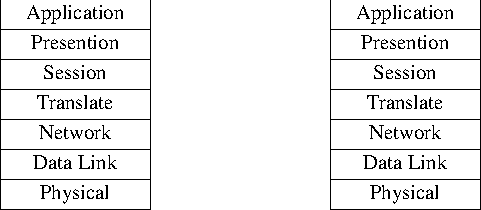
\includegraphics{graph/network01.pdf}
  \caption{网络七层模型}
\end{figure}

\section{安装Ansible}
\label{sec:InstallAnsible}

Ansible的安装很简单,配置好EPEL源后,就可以直接使用yum来进行安装了。

\begin{verbatim}
yum install -y ansible
\end{verbatim}

\section{测试Ansible}

确定我们的ansible可以正常使用,接下来,我们准备几台测试机器。由
于ansible是无agent的配置管理工具,在客户端无需安装任何额外程序,使
用SSH协议进行通信,而SSH是默认安装的。

为了今后方便进行配置管理,我们需要使用SSH无密码进行通信。本测试的几台主
机及主机名为:

\begin{table}[!ht]
  \centering
    \begin{tabular}{ll}
      \toprule
      主机           & 说明   \\
      \midrule
      192.168.56.150 & 主控端 \\
      192.168.56.111 & 被控端 \\
      192.168.56.112 & 被控端 \\
      \bottomrule
    \end{tabular}
    \caption{Ansible测试环境}
    \label{tab:AnsibleTestEnv}
\end{table}

在主控端生成SSH密钥对,并把公钥分发到被控端的机器上。
\begin{verbatim}
# ssh-keygen -t rsa
# ssh-copy-id -i /root/.ssh/id_rsa.pub root@192.168.56.111
# ssh-copy-id -i /root/.ssh/id_rsa.pub root@192.168.56.112
\end{verbatim}
以上配置完毕,我们来简单的使用一下。比如,ping测试一下我们的被控端是否
存活。
\begin{verbatim}
# cat /etc/ansible/hosts
[my1]
192.168.56.111
192.168.56.112

# ansible my1 -m ping 
192.168.56.111 | success >> {
    "changed": false, 
    "ping": "pong"
}

192.168.56.112 | success >> {
    "changed": false, 
    "ping": "pong"
}

命令说明:
   my1 -- ansible操作的对象,my1组里有2台机器
   -m  -- 表示使用的是ansible的哪个模块,默认是command模块
\end{verbatim}
\subsection{command模块}
\label{sec:AnsibleCommandMod}

使用command模块,可以执行一些比较简单的命令。command是ansible的默认模块,
我们要在一些机器上执行命令,可以省略“command”关键字。如果命令里包含空格,
需要使用引号以转义掉空格字符。较复杂的命令command模块并不支持,诸如,重
定向操作、管道操作等复杂操作command模块就无能为力了。下面看一些简单的例
子,
\begin{verbatim}
# ansible my1 -m command -a "uptime"
192.168.56.111 | success | rc=0 >>
 15:50pm  up   1:01,  2 users,  load average: 0.04, 0.03, 0.05

192.168.56.112 | success | rc=0 >>
 15:50pm  up   1:01,  2 users,  load average: 0.00, 0.01, 0.05

命令说明:
   -m command -- 表示使用command模块
   -a         -- 表示模块的参数
\end{verbatim}

\subsection{shell模块}
\label{sec:AnsibleShellMod}

shell模块与command模块类似,可以执行一些较为复杂的命令。支持诸如重定向
及管道的操作。下面看一个简单的例子,
\begin{verbatim}
# ansible my1 -m shell -a "cat /etc/hosts |grep -v '^#'"
192.168.56.111 | success | rc=0 >>
127.0.0.1	localhost 
192.168.56.111  puppetcamq1.local.site
192.168.56.112  puppetcamq2.local.site
192.168.56.202  puppetmaster
192.168.56.203  puppetca

192.168.56.112 | success | rc=0 >>
127.0.0.1	    localhost 
192.168.56.111	puppetslave
\end{verbatim}
\subsection{package模块}
\label{sec:AnsiblePackageMod}

Ansible有几种常见的包管理模块。比如Debian系列的系统上,使用的是apt包管
理机制;RHEL系列的系统上,使用的是yum包管理机制;SLES系列的系统上,使用
的是zypper包管理机制。那么,对应到Ansible中,对应的三个模块是apt模
块、yum模块、zypper模块。三种模块的使用方式一样,这里就使
用SUSE的zypper包管理方式。下面来看一个简单的例子,
\begin{verbatim}
# ansible my1 -m shell -a "service snmpd status"
192.168.56.111 | FAILED | rc=1 >>
service: no such service snmpd

192.168.56.112 | FAILED | rc=1 >>
service: no such service snmpd
\end{verbatim}
以上说明,这两台机器并没有安装net-snmp软件包。接下来,我们要安装之。
\begin{verbatim}
# ansible my1 -m zypper -a "name=net-snmp state=present"
192.168.56.112 | success >> {
    "changed": true, 
    "name": [
        "net-snmp"
    ], 
    "state": "present"
}

192.168.56.111 | success >> {
    "changed": true, 
    "name": [
        "net-snmp"
    ], 
    "state": "present"
}
\end{verbatim}
以上,已经安装net-snmp软件包,但是还没有启动。验证一下?
\begin{verbatim}
# ansible my1 -m shell -a "service snmpd status"
192.168.56.111 | FAILED | rc=3 >>
Checking for service snmpd:..unused

192.168.56.112 | FAILED | rc=3 >>
Checking for service snmpd:..unused

说明:
   在SUSE里,服务未启动,则是“unused”状态
\end{verbatim}

如何启动刚刚的snmpd服务呢?接下来看看service模块。

\subsection{service模块}
\label{sec:AnsibleServiceMod}

服务已经安装却迟迟不启动,这如何是好?使用service模块可以轻松搞定,
\begin{verbatim}
# ansible my1 -m service -a "name=snmpd state=running"
192.168.56.111 | success >> {
    "changed": true, 
    "name": "snmpd", 
    "state": "started"
}

192.168.56.112 | success >> {
    "changed": true, 
    "name": "snmpd", 
    "state": "started"
}
\end{verbatim}
根据输出,看上去是很美好,但是启动成功了吗?不会是在忽悠我们吧?你觉得
很有必要进行验证一把,我也是这么认为的。
\begin{verbatim}
# ansible my1 -m shell -a "service snmpd status"
192.168.56.111 | success | rc=0 >>
Checking for service snmpd:..running

192.168.56.112 | success | rc=0 >>
Checking for service snmpd:..running
\end{verbatim}
看来,Ansible并没有忽悠我们,确实把snmpd服务给启动了。但是这里的服务是
要开机启动的,该怎么办呢?看看帮助信息有没有相关的设置呢?结果小
白\footnote{小白就是ldczz2008@163.com}找到了enabled选项,可以满足此要求,
试试看?试之前,小白觉得还是有必要进行检查一下,snmpd服务是不是已经开机
自启了呢?我觉得不会,因为小白没有设置!
\begin{verbatim}
# ansible my1 -m shell -a "chkconfig -l |grep snmpd"
192.168.56.111 | success | rc=0 >>
snmpd           0:off  1:off  2:off  3:off  4:off  5:off  6:off

192.168.56.112 | success | rc=0 >>
snmpd           0:off  1:off  2:off  3:off  4:off  5:off  6:off
\end{verbatim}
snmpd服务安装完毕,确实没有设置开机自启,看来小白很是不专业,这么简单的
问题,却猜测不正确。接下来就查下帮助设置一下吧,可以使用enabled选项,
\begin{verbatim}
# ansible my1 -m service -a "name=snmpd enabled=yes"
# ansible my1 -m shell -a "chkconfig -l |grep snmpd"
192.168.56.111 | success | rc=0 >>
snmpd           0:off  1:off  2:on   3:on   4:off  5:on   6:off

192.168.56.112 | success | rc=0 >>
snmpd           0:off  1:off  2:on   3:on   4:off  5:on   6:off
\end{verbatim}
\subsection{file模块}
\label{sec:AnsibleFileMod}

file模块一般是对远程主机上的文件或目录进行操作的。可以创建软、硬链接,
修改文件属组及权限等。下面看一个例子,把/etc/hosts文件链接到/tmp目录
下,
\begin{verbatim}
# ansible my1 -m file -a "src=/etc/hosts dest=/tmp/hosts state=link"
192.168.56.111 | success >> {
    "changed": true, 
    "dest": "/tmp/hosts", 
    "mode": "0777", 
    "owner": "root", 
    "src": "/etc/hosts", 
    "state": "link"
}

192.168.56.112 | success >> {
    "changed": true, 
    "dest": "/tmp/hosts", 
    "mode": "0777", 
    "owner": "root", 
    "src": "/etc/hosts", 
    "state": "link"
}
\end{verbatim}

接下来,验证一下是不是已经创建软链接了,

\begin{verbatim}
# ansible my1 -m shell -a "egrep -v '^#|^$' /tmp/hosts"
192.168.56.111 | success | rc=0 >>
127.0.0.1	    localhost 
192.168.56.111  puppetcamq1.local.site
192.168.56.112  puppetcamq2.local.site
192.168.56.202  puppetmaster
192.168.56.203  puppetca

192.168.56.112 | success | rc=0 >>
127.0.0.1	    localhost 
192.168.56.111	puppetslave
\end{verbatim}
有了以上输出,说明没有问题!file模块就介绍这么多吧!如果我们有需要向远
程主机发送文件该怎么办呢?可以使用copy模块,接下来的一个小节,来感受一
下copy模块。

\subsection{copy模块}
\label{AnsibleCopyMod}

copy模块是用向远程主机推送文件或目录用的。在推送过程中,我们可以设置文
件在远程主机上的一些属性,如所有者、所属组等。接下来看操作,首先在控制
端准备test.sh文件,
\begin{verbatim}
# cat /root/test.sh 
#!/bin/bash

echo -n "Today is: " 
date +%F\ %H:%M:%S

echo -n "My name is: "
hostname
\end{verbatim}
然后,把文件推送到远程主机的/tmp目录下,并设置权限,
\begin{verbatim}
# ansible my1 -m copy -a "src=/root/test.sh \
> dest=/tmp/test.sh owner=root group=root \
> mode=0755"
192.168.56.111 | success >> {
    "changed": true, 
    "dest": "/tmp/test.sh" 
}

192.168.56.112 | success >> {
    "changed": true, 
    "dest": "/tmp/test.sh" 
}
\end{verbatim}

根据输出,我们可以看出,在主控端的test.sh文件已经复制过去了,并且修改了
相应的权限。小白不高兴再次去做验证了,接下来就直接执行这个脚本吧!
\begin{verbatim}
# ansible my1 -m shell -a "/tmp/test.sh"
192.168.56.111 | success | rc=0 >>
Today is: 2015-07-01 15:02:58
My name is: puppetcamq1

192.168.56.112 | success | rc=0 >>
Today is: 2015-07-01 15:03:01
My name is: puppetslave
\end{verbatim}
小白由于好奇,这个脚本之所以可以执行成功,是因为我们指定了其权限为755,
其文件的所有者、所属组及其他用户皆可执行该文件。接下来,设置其权限
为644呢,是否可以执行呢?试试呗,试一下机器又不会爆炸,
\begin{verbatim}
# ansible my1 -m file -a "path=/tmp/test.sh mode=0644"
192.168.56.111 | success >> {
    "changed": true, 
    "mode": "0644", 
    "owner": "root", 
    "path": "/tmp/test.sh", 
    "state": "file"
}

192.168.56.112 | success >> {
    "changed": true, 
    "mode": "0644", 
    "owner": "root", 
    "path": "/tmp/test.sh", 
    "state": "file"
}
\end{verbatim}
通过上述设置及其输出情况,我们可以看到,test.sh文件的权限已经修改为
了644。执行一下吧,
\begin{verbatim}
# ansible my1 -m shell -a "/tmp/test.sh"
192.168.56.111 | FAILED | rc=126 >>
/bin/sh: /tmp/test.sh: Permission denied

192.168.56.112 | FAILED | rc=126 >>
/bin/sh: /tmp/test.sh: Permission denied
\end{verbatim}

这样执行呢?

\begin{verbatim}
# ansible my1 -m shell -a "bash /tmp/test.sh"
192.168.56.111 | success | rc=0 >>
Today is: 2015-07-01 15:09:47
My name is: puppetcamq1

192.168.56.112 | success | rc=0 >>
Today is: 2015-07-01 15:09:50
My name is: puppetslave
\end{verbatim}
这个例子很是无聊,主要是小白想让大家熟悉一下file模块而已。file模块是从
本地主机向远程主机推送文件,可不可以从远程主机拉取文件呢?答案是可以的!
可以使用fetch模块实现该需求。这里不再演示。

\subsection{lineinfile模块}
\label{AnsibleLineinfileMod}

\subsection{setup模块}
\label{AnsibleSetupMod}

setup模块里包含了很多有用的变量。在执行playbooks时,这些变量可以
被playbooks来调用,有了这些变量,可以编排复杂的任务。setup模块默认是输
出所有远程主机上的变量信息,我们可以通过filter来过滤我们想要的信息。举
个例子看看,如只显示网卡信息,
\begin{verbatim}
# ansible my1 -m setup -a "filter=ansible_eth[0-2]"
192.168.56.112 | success >> {
    "ansible_facts": {
        "ansible_eth1": {
            "device": "eth1"
        }, 
        "ansible_eth2": {
            "device": "eth2"
    },
}

192.168.56.111 | success >> {
    "ansible_facts": {
        "ansible_eth0": {
            "device": "eth0", 
            }, 
        "ansible_eth1": {
            "device": "eth1"
    }
}
\end{verbatim}

\begin{verbatim}
# ansible my1 -m setup -a "filter=ansible_kernel"
192.168.56.112 | success >> {
    "ansible_facts": {
        "ansible_kernel": "3.0.13-0.27-default"
    }, 
    "changed": false
}

192.168.56.111 | success >> {
    "ansible_facts": {
        "ansible_kernel": "3.0.13-0.27-default"
    }, 
    "changed": false
}
\end{verbatim}

\subsection{获得模块的帮助信息}
\label{sec:AnsibleGetModHelp}

安装完毕ansible,同时也安装了ansible的帮助文档。可以通过ansible-doc命令
来查看,后面跟具体模块的名称。ansible有哪些模块呢?可以使
用“ansible-doc -l”命令来查看,由于输出内容较多,这里就不演示了。在本测
试环境中,ansible的模块有259个,已足够我们目前的使用了。

我们只介绍了如何进行安装服务及查询状态的操作,并没有介绍如何卸载服务、
删除软硬链接、修改文件权限等操作,更多的内容留给大家自己动手去实践,完
全可以通过帮助信息来自己完成。

\section{Ansible工作流程}
\label{sec:AnsibleWorkflow}

\section{playbooks}

\section{一个综合实例}
\label{chap:ComplexInstance}

由第一章的内容

\begin{figure}[htbp]
  \centering
  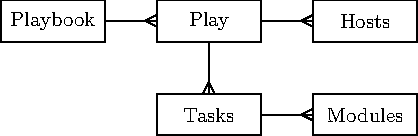
\includegraphics{graph/ansible-0.pdf}
  \caption{Playbook}
  \label{fig:PlaybookRelition}
\end{figure}

该实例的目录结构为:
\begin{verbatim}
# tree playbooks/
playbooks/
|-- group_vars
|   \-- all
|-- hosts
|-- roles
|   \-- common
|       |-- handlers
|       |   \-- main.yml
|       |-- tasks
|       |   \-- main.yml
|       |-- templates
|       |   |-- net-snmp.j2
|       |   |-- ntp.conf.j2
|       |   |-- snmpd.conf.j2
|       |   \-- zypper.repo.j2
|       \-- vars
|           \-- main.yml
\-- site.yml
\end{verbatim}

\begin{verbatim}
# cat playbooks/group_vars/all
---
# Variables listed here are applicable to all host groups
ntpserver: 172.16.25.35
\end{verbatim}

该实例所执行的主机为,
\begin{verbatim}
# cat playbooks/hosts
[bigdata]
172.17.25.31
172.17.25.39
172.17.25.40
\end{verbatim}

\begin{verbatim}
# cat playbooks/common/tasks/main.yml
---
- name: Prepare zyyper repo file
  template: src=zypper.repo.j2 dest=/etc/zypper/repos.d/suse11sp2.repo

- name: Install net-snmp package
  zypper: pkg=net-snmp state=latest

- name: Modify snmp configuration file
  template: src=snmpd.conf.j2 dest=/etc/snmp/snmpd.conf

- name: Modify ntp configuration file
  template: src=ntp.conf.j2 dest=/etc/ntp.conf

- name: Restart ntp service
  shell: /etc/init.d/ntp restart

- name: Enable ntp service
  shell: chkconfig ntp on

- name: Restart snmpd service
  shell: service snmpd restart

- name: Enable snmpd service
  shell: chkconfig snmpd on
\end{verbatim}

\begin{verbatim}
# cat playbooks/common/handlers/main.yml
---
- name: restart snmpd
  service name=snmpd state=restarted enabled=yes

- name: restart ntp
  service: name=ntp state=restarted enabled=yes
\end{verbatim}

snmp日志轮询配置模板,
\begin{verbatim}
# cat playbooks/common/templates/net-snmp.j2
/var/log/net-snmpd.log {
   daily
   compress
   dateext
   maxage 10
   logrotate 10
   size=+1024k
   notifempty
   missingok
   sharedscripts
   postrotate
       /etc/init.d/snmpd reload ||:
	   if [ -x /etc/init.d/snmptrapd ] ; then \
	      /etc/init.d/snmptrapd reload ||: ; \
	   fi
   endscript
}
\end{verbatim}

NTP服务的配置模板,
\begin{verbatim}
# cat playbooks/common/templates/ntp.conf.j2
driftfile /var/lib/ntp/drift/ntp.drift
logfile   /var/log/ntp
server    {{ ntpserver }}
\end{verbatim}

SNMP服务的配置模板,
\begin{verbatim}
# cat playbooks/common/templates/snmpd.conf.j2
rocommunity public
\end{verbatim}

YAST源的配置模板,
\begin{verbatim}
# cat playbooks/common/templates/zypper.repo.j2
name=SUSE-Linux-Enterprise-Server-11-SP2 11.2.2-1.234
enabled=1
autorefresh=1
baseurl=ftp://{{ yastserver }}/
path=/
type=yast2
keeppackages=0
\end{verbatim}

变量文件内容为,
\begin{verbatim}
# cat playbooks/common/vars/main.yml
---
ntpserver: 172.16.25.35
yastserver: 172.16.25.35
\end{verbatim}

该实例的入口文件为,
\begin{verbatim}
# cat playbooks/site.yml
---
- name: apply common configuation to all nodes
  hosts: all
  roles:
  - common
\end{verbatim}

%%% Local Variables:
%%% mode: latex
%%% TeX-master: t
%%% End:


% 自动化运维工具fabric
\chapter{fabric}
\label{chap:fabric}

%%% Local Variables:
%%% mode: latex
%%% TeX-master: t
%%% End:


% 自动化运维工具saltstack
\chapter{SaltStack}
\label{chap:chapSalt}

This data coming from the minion (e.g., operating system) is called
grains. But there is another type of data: pillar data. While grains
are advertised by the minion back to the master, pillar data is stored
on the master and is made available to each minion individually; that
is, a minion cannot see any pillar data but its own. It is common for
people new to Salt to ask about grains versus pillar data, so we will
discuss them further in Chapter 5. For the moment, you can think of
grains as metadata about the host (e.g., number of CPUs), while pillar
is data the host needs (e.g., a database password). In other words, a
minion tells the master what its grains are, while the minion asks the
master for its pillar data. For now, just know that you can use either
to define the target for a command.

\section{初识SaltStack}
\label{sec:basicSalt}

\begin{figure}[!htbp]
  \centering
  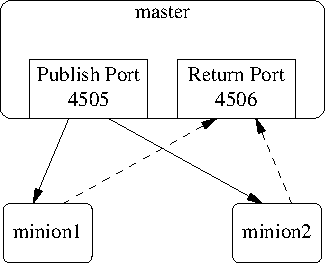
\includegraphics{graph/saltstack_communication.pdf}
  \caption{salt通信示意图}
  \label{fig:saltRelition}
\end{figure}

\section{安装及运行SaltStack}
\label{sec:installSalt}

\subsection{环境准备}
\label{sec:saltEnvPrepare}

以下测试是在CentOS6U5 64位系统上进行测试。系统均关闭iptables及selinux,
如果要开启iptables,请设置允许开放本机的53端口。

\begin{table}[htbp]
  \centering
    \caption{SaltStack测试环境机器列表}
    \label{tab:saltTestMachineList}
    \begin{tabular}{llr}
      \toprule
      主机名     & IP地址 & 说明 \\
      \midrule
      master01.lavenliu.com  & 192.168.20.134 &  Salt Master \\
      minion01.lavenliu.com  & 192.168.20.135 &  Salt Minion \\
      minion02.lavenliu.com  & 192.168.20.136 &  Salt Minion \\
      \bottomrule
    \end{tabular}
\end{table}

假设已经做了DNS解析,如果没有做DNS解析,请在/etc/hosts文件里设置静态主机名解析。
这里使用DNS的方式进行主机名的解析工作,解析测试如下:

\begin{verbatim}
[root@master01 ~]# nslookup master01.lavenliu.com
Server:		192.168.20.134
Address:	192.168.20.134#53

Name:	master01.lavenliu.com
Address: 192.168.20.134

[root@master01 ~]# nslookup minion01.lavenliu.com
Server:		192.168.20.134
Address:	192.168.20.134#53

Name:	minion01.lavenliu.com
Address: 192.168.20.135

[root@master01 ~]# nslookup minion02.lavenliu.com
Server:		192.168.20.134
Address:	192.168.20.134#53

Name:	minion02.lavenliu.com
Address: 192.168.20.136
\end{verbatim}

\subsection{安装SaltStack Master}
\label{sec:installSaltMaster}

使用yum进行salt-master的安装,

\begin{verbatim}
[root@master01 ~]# yum install -y salt-master
\end{verbatim}

将salt-master加入开机自启动,

\begin{verbatim}
[root@master01 ~]# chkconfig salt-master on
\end{verbatim}

\subsection{安装SaltStack Minion}
\label{sec:installSaltMinion}

使用yum进行salt-minion的安装,在minion01及minion02两台机器上进行操作,

\begin{verbatim}
# yum install -y salt-minion
\end{verbatim}

将salt-minion加入开机自启动,在minion01及minion02两台机器上进行操作,

\begin{verbatim}
# chkconfig salt-minion on
\end{verbatim}

\section{SaltStack配置}
\label{sec:saltConfigure}

\subsection{Master端配置}
\label{sec:masterConfigure}

\subsection{Minion端配置}
\label{sec:minionConfigure}

\section{基本使用}
\label{sec:basicUsage}

\subsection{单master设置}
\label{sec:singleMasterSetup}

\subsection{基本命令}
\label{sec:basicSaltCommand}

\subsection{密钥管理}
\label{sec:saltKeyManagement}

\subsection{定位minions}
\label{sec:minionTargeting}

当我们有成千上万台机器时,这些机器承担着不同的角色。有的是HTTP服务器,
有的是DB服务器,有的是文件共享服务器。而且它们分别运行不同的操作系统,
比如,HTTP服务器运行在CentOS系统之上;DB服务器运行在SUSE系统之上;文件
共享服务器运行在FreeBSD系统之上。当我们想在所有的服务器上增加work账号
时,那将是很简单的一件事情。如果WEB服务器只安装httpd,DB服务器只安装
MySQL,文件共享服务器只安装NFS等,如何操作呢?Salt提供了多种选项来帮助
我们定位minions。

\subsubsection*{Minion ID}

最简单的方式就是通过指定具体的minion ID来定位目标机器。如,

\begin{verbatim}
# salt automatic01 test.ping
automatic01:
    True
\end{verbatim}

\subsubsection*{List(-L)选项}

另外,我们可以使用salt命令的\verb|-L|选项,向salt提供一组Minion ID的列
表,如,

\begin{verbatim}
# salt -L mha-manager,automatic01 test.ping
mha-manager:
    True
automatic01:
    True
\end{verbatim}

\subsubsection*{通配符\*}

我们还可以shell-style的通配符,通配符被替换成一组已签过名的minions。\*
表示所有已签名的minions。如,

\begin{verbatim}
# salt '*' test.ping
windows01:
    True
mha-manager:
    True
automatic01:
    True
debian:
    True
\end{verbatim}

通过输出结果,可以看出,这些minions并不是按列表顺序返回的,而是按谁先
返回数据的顺序返回的。

我们还可以使用通配符并结合minions ID一起使用,如,

\begin{verbatim}
# salt 'auto*' test.ping
automatic01:
    True
\end{verbatim}

\subsubsection*{Regular Expression(-E)}

我们可以使用正则表达式来匹配更精确的minions,如,

\begin{verbatim}
# salt -E '.*01' test.ping
windows01:
    True
automatic01:
    True
\end{verbatim}

\subsubsection*{Grains(-G)}

Grains是一组关于操作系统的信息,是在minions启动时加载的,是静态的数据。
Grains提供了操作系统名称和操作系统版本号等。我们可以基于此,只在
CenOS6.5的机器上安装httpd软件包。

如何使用呢?如,

\begin{verbatim}
# salt -G 'os:CentOS' test.ping
automatic01:
    True
mha-manager:
    True
\end{verbatim}

\subsubsection*{Compound(-C)}

接下来的这种方式更为强大一些。它允许我们以组合的形式来匹配minioins。接
下来看一个简单的例子,如,

\begin{verbatim}
# salt -C 'auto* or G@os:Debian' test.ping
automatic01:
    True
debian:
    True

# salt -C 'auto* or L@debian,windows01' test.ping
windows01:
    True
automatic01:
    True
debian:
    True
\end{verbatim}

\section{理解YAML}
\label{sec:understandYAML}

SLS文件的默认渲染器是YAML渲染器。书写SLS文件只有简单的三条规则。

\section{SaltStack配置管理实例}
\label{sec:saltDeployInstances}

接下来,就实际的运用以上的知识点,写出一些可工作的配置管理规则以进行配置管理。只要我们编排好SLS文件,Salt就会按照我们的编排进行自动的配置管理。

看一下目录结构:

\begin{verbatim}
[root@master01 states]# pwd
/etc/salt/states
[root@master01 states]# tree
.
├── init
│   ├── files
│   │   ├── limits.conf
│   │   └── vimrc
│   ├── pkg.sls
│   ├── test.sls
│   └── vim.sls
├── prod
│   ├── elk
│   │   ├── elasticsearch.sls
│   │   ├── files
│   │   │   ├── elasticsearch-1.7.0.tar.gz
│   │   │   ├── elasticsearch_plugins.tar.gz
│   │   │   ├── elasticsearch.yml
│   │   │   ├── es-service.tar.gz
│   │   │   ├── indexer.conf
│   │   │   ├── kibana-4.1.1-linux-x64.tar.gz
│   │   │   ├── logstash-1.5.3.tar.gz
│   │   │   ├── logstash-2.3.1-1.noarch.rpm
│   │   │   ├── logstash.sh
│   │   │   ├── master.tar.gz
│   │   │   └── shipper.conf
│   │   ├── indexer.sls
│   │   ├── install.sls
│   │   ├── kibana.sls
│   │   ├── logstash.sls
│   │   └── shipper.sls
│   ├── haproxy
│   │   ├── files
│   │   │   ├── haproxy-1.5.15.tar.gz
│   │   │   └── haproxy.init
│   │   └── install.sls
│   ├── jdk
│   │   ├── files
│   │   │   └── jdk-8u65-linux-x64.tar.gz
│   │   └── install.sls
│   ├── keepalived
│   │   └── files
│   │       └── keepalived-1.2.16.tar.gz
│   ├── libevent
│   │   ├── files
│   │   │   └── libevent-2.0.22-stable.tar.gz
│   │   └── install.sls
│   ├── logstash.zip
│   ├── memcached
│   │   ├── files
│   │   │   └── memcached-1.4.25.tar.gz
│   │   ├── install.sls
│   │   └── service.sls
│   ├── mysql
│   │   ├── files
│   │   │   └── mysql-5.5.32.tar.gz
│   │   └── install.sls
│   ├── nginx
│   │   └── files
│   ├── pkg
│   │   └── pkg-init.sls
│   ├── redis
│   │   ├── files
│   │   │   └── redis.conf
│   │   └── server.sls
│   └── tomcat
│       ├── files
│       │   └── apache-tomcat-8.0.28.tar.gz
│       └── install.sls
└── top.sls

27 directories, 76 files
\end{verbatim}

\subsection{安装JDK}
\label{sec:saltInstallJDK}

\begin{verbatim}
[root@master01 states]# cat prod/jdk/install.sls 
jdk-install:
  file.managed:
    - name: /usr/local/src/jdk-8u65-linux-x64.tar.gz
    - source: salt://prod/jdk/files/jdk-8u65-linux-x64.tar.gz
    - user: root
    - group: root
    - mode: 644
  cmd.run:
    - name: cd /usr/local/src && tar -xf jdk-8u65-linux-x64.tar.gz && mv jdk1.8.0_65 jdk && chown -R root:root jdk
    - unless: test -d /usr/local/jdk

/etc/profile:
  file.append:
    - text:
      - export JAVA_HOME=/usr/local/jdk
      - export JRE_HOME=${JAVA_HOME}/jre
      - CLASS_PATH=${JAVA_HOME}/lib:${JRE_HOME}/lib
      - PATH=$PATH:$JAVA_HOME/bin
\end{verbatim}

\subsection{安装Tomcat}
\label{sec:saltInstallTomcat}

\subsection{安装Nginx}
\label{sec:saltInstallNginx}

\subsection{安装MySQL}
\label{saltInstallMySQL}

\subsection{安装PHP}
\label{sec:saltInstallPHP}

\subsection{安装Redis}
\label{sec:saltInstallRedis}

\subsection{安装ELK Stack}
\label{sec:saltInstallELK}

\subsection{安装OpenStack}
\label{sec:saltInstallOpenStack}


%%% Local Variables:
%%% mode: latex
%%% TeX-master: t
%%% End:


% 自动化运维工具puppet
\chapter{Puppet}

\section{关于Puppet}

\section{服务器端puppetca安装配置}

多台同构或异构的计算机用某种方式连接起来协同完成特定的任务就构成了集群
系统,目前Linux下的集群主要有三种类型:

\subsection{配置NTP}
\label{sec:NTPconf}

\subsection{增加虚拟IP}
\label{sec:AddVIP}

\subsection{主机名IP静态解析配置和验证}
\label{sec:StaticIP}

\subsection{安装新版本puppet软件包}
\label{sec:InstallNewPuppet}

\subsection{修改配置并验证结果}
\label{sec:ModifyConfVerify}

\section{客户端puppet安装配置}

\section{服务器端rabbitmq-server安装配置}

\section{服务器端mcollective安装配置}

\section{客户端mcollective安装配置}

%%% Local Variables:
%%% mode: latex
%%% TeX-master: t
%%% End:


\chapter{Git}

\section{git简介}

Git是一款分布式版本控制系统,有别于CVS和SVN等集中式版本控制系统,Git可
以让研发团队更加高效地协同工作,从而提高生产率。使用Git,开发人员的工作
不会因为频繁地遭遇提交冲突而中断,管理人员也无须为数据的备份而担心。

\section{安装git}

\begin{verbatim}
# Debian系列
sudo apt-get install git
sudo apt-get install git-core

# RHEL系列
yum install git
\end{verbatim}

\section{创建版本库}
设置用户名及邮件地址,
\begin{verbatim}
git config --global user.name "Laven Liu"
git config --global user.email "air.man.six@gmail.com"
git config --global color.ui true
\end{verbatim}

查看已配置的信息,
\begin{verbatim}
git config --global user.name
Laven Liu

git config --global user.email
air.man.six@gmail.com

git config --list
git config --global --list
\end{verbatim}

\section{本地仓库}

什么是版本库呢?版本库又名仓库,英文名repository,我们可以简单理解成一个
目录,这个目录里面的所有文件都可以被Git管理起来,每个文件的修改、删
除,Git都能跟踪,以便任何时刻都可以追踪历史,或者在将来某个时刻可以“还
原”。

所以,创建一个版本库非常简单,首先,选择一个合适的地方,创建一个空目
录:

\begin{verbatim}
$ mkdir learngit
$ cd learngit
$ pwd
/home/richard/learngit
\end{verbatim}

pwd命令用于显示当前目录。在我的Ubuntu上,这个仓库位
于/home/richard/learngit。

如果你使用Windows系统,为了避免遇到各种莫名其妙的问题,请确保目录名(包
括父目录)不包含中文。

第二步,通过git init命令把这个目录变成Git可以管理的仓库:

\begin{verbatim}
$ git init
\end{verbatim}

瞬间Git就把仓库建好了,而且告诉你是一个空的仓库(empty Git repository),
细心的读者可以发现当前目录下多了一个.git的目录,这个目录是Git来跟踪管理
版本库的,没事千万不要手动修改这个目录里面的文件,不然改乱了,就把Git仓
库给破坏了。

首先这里再明确一下,所有的版本控制系统,其实只能跟踪文本文件的改动,比
如TXT文件,网页,所有的程序代码等等,Git也不例外。版本控制系统可以告诉
你每次的改动,比如在第5行加了一个单词“Linux”,在第8行删了一个单
词“Windows”。而图片、视频这些二进制文件,虽然也能由版本控制系统管理,但
没法跟踪文件的变化,只能把二进制文件每次改动串起来,也就是只知道图片
从100KB改成了120KB,但到底改了啥,版本控制系统不知道,也没法知道。

不幸的是,Microsoft的Word格式是二进制格式,因此,版本控制系统是没法跟
踪Word文件的改动的,前面我们举的例子只是为了演示,如果要真正使用版本控
制系统,就要以纯文本方式编写文件。

因为文本是有编码的,比如中文有常用的GBK编码,日文有Shift\_JIS编码,如果
没有历史遗留问题,强烈建议使用标准的UTF-8编码,所有语言使用同一种编码,
既没有冲突,又被所有平台所支持。

言归正传,现在我们编写一个readme.txt文件,内容如下:

\begin{verbatim}
$ cat readme.txt
Git is a version control system.
Git is free software.
\end{verbatim}

一定要放到learngit目录下(子目录也行),因为这是一个Git仓库,放到其他地
方Git再厉害也找不到这个文件。

和把大象放到冰箱需要3步相比,把一个文件放到Git仓库只需要两步。

第一步,用命令git add告诉Git,把文件添加到仓库:

\begin{verbatim}
$ git add readme.txt
\end{verbatim}

执行上面的命令,没有任何显示,这就对了,Unix的哲学是“没有消息就是好消
息”,说明添加成功。

第二步,用命令git commit告诉Git,把文件提交到仓库:

\begin{verbatim}
$ git commit -m "wrote a readme file"
[master (root-commit) cb926e7] wrote a readme file
 1 file changed, 2 insertions(+)
 create mode 100644 readme.txt
\end{verbatim}

简单解释一下\verb|git commit|命令,\verb|-m|后面输入的是本次提交的说明,
可以输入任意内容,当然最好是有意义的,这样你就能从历史记录里方便地找到
改动记录。

嫌麻烦不想输入\verb|-m "xxx"|行不行?确实有办法可以这么干,但是强烈不建
议你这么干,因为输入说明对自己对别人阅读都很重要。实在不想输入说明的童
鞋请自行Google,我不告诉你这个参数。

\verb|git commit|命令执行成功后会告诉你,1个文件被改动(我们新添加
的readme.txt文件),插入了两行内容(readme.txt有两行内容)。

为什么Git添加文件需要add,commit一共两步呢?因为commit可以一次提交很多
文件,所以你可以多次add不同的文件,比如:

\begin{verbatim}
$ git add file1.txt
$ git add file2.txt
$ git add file3.txt
$ git commit -m "add 3 files."
\end{verbatim}

\subsection{版本回退}

\subsection{工作区和暂存区}

\subsection{管理修改}

\subsection{撤销修改}

\subsection{删除文件}

\section{远程仓库}

\subsection{添加远程库}

\subsection{克隆远程库}

\section{分支管理}

\subsection{创建与合并分支}

\subsection{解决冲突}

\subsection{分支管理策略}

\subsection{Bug分支}

\subsection{Feature分支}

\subsection{多人协作}

\section{标签管理}

\subsection{创建标签}

\subsection{操作标签}

\section{使用GitHub}

\section{自定义Git}

\subsection{忽略特殊文件}

\subsection{配置别名}

\subsection{搭建Git服务器}


\part{虚拟化及云计算部分}
\label{part:virtualization}

虚拟化的主要目标是在一台主机上运行多个操作系统,以便充分利用大型机上昂
贵的计算资源。随着x86处理器的性能提升以及应用的普及,虚拟化技术的发展也
开始进入到x86架构领域。特别是到20世纪90年代末期,VMware等虚拟化软件厂商
为x86平台上虚拟化技术应用开辟了道路,提供了以VMM(Virtual Machine
  Monitor)为中心,对PC服务器平台虚拟化的软件解决方案。纯软件解决方案在
性能方面的瓶颈后来又进一步催生出了半虚拟化技术和硬件虚拟化技术,最终
Intel的VT(Virtualization Technology,虚拟化技术)和AMD的SVM(Secure
  Virtual Machine,安全虚拟机)技术均在硬件级提供了对虚拟化的支持。虚拟
化技术被列为2009年度最值得关注的IT技术之首,足可见虚拟化技术在目前企业
计算和应用领域的重要性。

% kvm章节
\chapter{KVM}
\label{chap:kvm}

KVM(Kernel-based Virtual Machin)的简称)是一个开源的系统虚拟化模块,
自Linux 2.6.20之后集成在Linux的各个主要发行版本中。它使用Linux自身的调
度器进行管理,所以相对于Xen,其核心源码很少。KVM目前已成为学术界的主
流VMM之一。

\section{关于KVM}
\label{sec:AboutKVM}

KVM是开源软件,全称是Kernel-based virtual machine(基于内核的虚拟机),
是x86架构且硬件支持虚拟化技术(如Intel VT-x或AMD-V)的Linux全虚拟化解决
方案。KVM包含一个为处理器提供底层虚拟化,可加载的核心模
块kvm.ko(kvm-intel.ko或kvm-amd.ko)。KVM还需要一个经过修改
的QEMU软件qemu-kvm,作为虚拟机上层控制和界面。

KVM能在不改变Linux或Windows镜像的情况下同时运行多个虚拟机(多个虚拟机使
用同一个镜像),并为每一个虚拟机配置个性化硬件环境(网卡、磁盘、图形适
配器等)。

在主流的Linux内核,如2.6.20以上的内核版本均已包含了KVM核心。

\subsection{KVM管理工具libvirt简介}
\label{sec:libvirtIntro}

libvirt是目前使用最为广泛的KVM虚拟机管理工具和应用程序接口(API),而且
一些常用虚拟机的管理工具(如virsh、virt-install及virt-manager等)和云计
算框架平台(如OpenStack、OpenNubla等)都在底层使用libvirt的应用程序接
口。

libvirt是为了更方便地管理平台虚拟化技术而设计的开放源代码的应用程序接口、
守护进程和管理工具,它不仅提供了对虚拟化客户机的管理,也提供了对虚拟化
网络和存储的管理。

libvirt的应用程序接口已被广泛地用在基于虚拟化和云计算的解决方案中,主要
作为连接底层Hypervisor和上层应用程序的一个中间适配层。libvirt对多种不同
的Hypervisor的支持是通过一种基于驱动程序的架构来实现的。libvirt对不同
的Hypervisor提供了不同的驱动:对Xen有Xen的驱动,对QEMU/KVM有QEMU驱动;
对VMware有VMware的驱动。libvirt作为中间适配层,让底层Hypervisor对上层用
户空间的管理工具是可以做到完全透明的,因为libvirt屏蔽了底层各
种Hypervisor的细节,为上层管理工具提供了一个统一的API接口。通过libvirt,
一些用户空间的管理工具可以管理各种不同的Hypervisor和其上面运行的客户机,
它们之间的交互拓扑如下图所示:

\begin{figure}[ht]
  \centering
  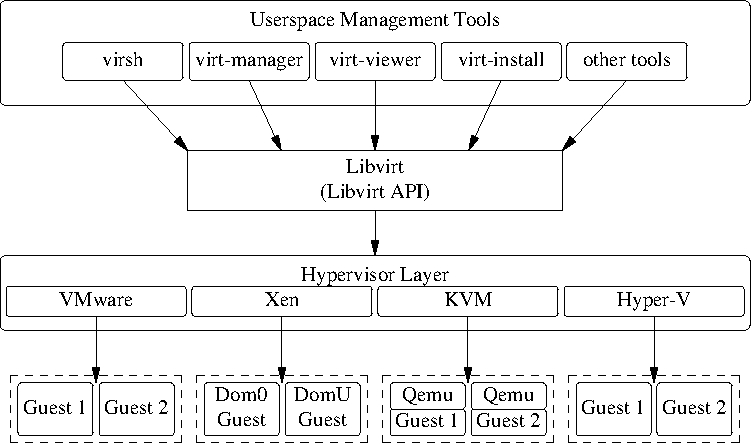
\includegraphics{graph/libvirt_support.pdf}
  \caption{\label{fig:libvirtSupport} Libvirt支持的虚拟化类型}
\end{figure}

\subsection{libvirt中的一些术语}
\label{sec:libvirtTerm}

1. 节点(Node):一台物理机;上面可能运行多个虚拟客户机,Hypervisor和Domain都运行在节点之上。

2. Hypervisor:也称虚拟机监视器(VMM),如KVM、Xen、VMware、Hyper-V等,是虚拟化中的一个底层软件层,它可以虚拟化一个节点让其运行多个虚拟客户机(不同的客户机有可能运行不同的操作系统)。

3. 域(Domain):是Hypervisor上运行的一个客户机操作系统实例。域也被称为实例、客户机操作系统(Guest OS)、虚拟机(Virtual Machine),它们都是指同一个概念。

节点、Hypervisor及域三者之间的关系如下图所示:

\begin{figure}[htbp]
  \centering
  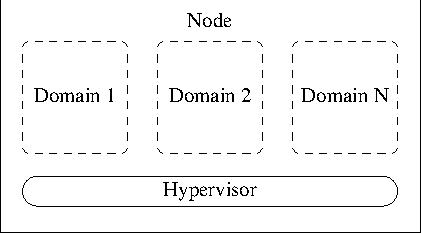
\includegraphics{graph/libvirt_node_hypervisor_domain.pdf}
  \caption{\label{fig:libvirtNodeHyperDomain} 节点、域与Hypervisor之间的关系}
\end{figure}

\subsection{检查宿主机是否支持KVM虚拟化}
\label{sec:checkIfSupportKVM}

\begin{verbatim}
# grep -E --color '(vmx|svm)' /proc/cpuinfo
\end{verbatim}

如果有红色的字符输出,说明系统支持虚拟化,然后接下来的一些操作才是有意
义的。

\section{安装前的准备工作}
\label{sec:kvmPrepare}

\subsection{KVM测试环境}
\label{sec:testEnv}

下面的操作是在VMWare的两台虚拟机上进行的,

测试环境为:

安装EPEL源

\subsection{安装EPEL源}
\label{sec:InstallEpel}

\begin{verbatim}
# rpm -ivh http://mirrors.ustc.edu.cn/fedora/epel//6/x86_64/epel-release-6-8.noarch.rpm
\end{verbatim}

\subsection{安装KVM管理工具}
\label{sec:InstallKvmManager}

为了使用KVM虚拟化,操作系统至少要安装qemu-kvm及qemu-img两个软件包,这两
个软件包在宿主机上为提使用者提供了用户层的KVM模拟器和硬盘镜像管理工具。
因此,这两个软件包是必须安装的,操作如下:

\begin{verbatim}
# yum install -y qemu-kvm qemu-img
\end{verbatim}

另外还有几个建议安装的软件包,如下:

安装以上建议的软件包:

\begin{verbatim}
# yum install virt-manager \
libvirt \
libvirt-python \
python-virtinst \
libvirt-client
\end{verbatim}

\section{开始部署KVM虚拟机}
\label{sec:beginKVM}

有了上面的准备工作,接下来就可以创建虚拟机了。

\subsection{创建虚拟机镜像}
\label{sec:createVmImg}

虚拟机镜像文件就是QEMU(KVM)虚拟机使用的硬盘文件格式。

\subsubsection{创建raw格式镜像文件}
\label{sec:createRawImg}

这里新建一个5G的RAW格式的虚拟镜像文件,可以根据具体业务设置镜像文件大小,

\begin{verbatim}
# qemu-img create -f raw /opt/lavenliu.raw 5G
Formatting '/opt/lavenliu.raw', fmt=raw size=5368709120
\end{verbatim}

创建完毕,可以查看刚才新建的虚拟机镜像文件,

\begin{verbatim}
# qemu-img info /opt/lavenliu.raw 
image: /opt/lavenliu.raw
file format: raw
virtual size: 5.0G (5368709120 bytes)
disk size: 0
\end{verbatim}

\subsubsection{创建qcow2格式镜像文件}
\label{sec:createQcow2Img}

创建qcow2格式的镜像文件与创建raw格式的镜像文件步骤一样,只是\verb|-f|选
项后面指定的虚拟机镜像文件格式不一样而已。操作如下:

\begin{verbatim}
# qemu-img create -f qcow2 /opt/taoqi.qcow2 5G
Formatting '/opt/taoqi.qcow2', fmt=qcow2 size=5368709120 encryption=off cluster_size=65536
\end{verbatim}

查看刚创建的虚拟机镜像文件,

\begin{verbatim}
# qemu-img info /opt/taoqi.qcow2 
image: /opt/taoqi.qcow2
file format: qcow2
virtual size: 5.0G (5368709120 bytes)
disk size: 1.4G
cluster_size: 65536
\end{verbatim}

format指镜像的格式,常用的格式为raw和qcow2,如果不声明,默认为raw模式,
但推荐使用qcow2格式。

\subsubsection{虚拟机镜像文件格式对比}
\label{sec:createImgContrast}

1.	raw格式:可以简单、容易地导出到其它模拟器中,但是立即分配占用空间大。
2.	qcow2格式:是qcow格式的升级版本,是目前最万能的格式。使用它可获得较小映像,也是虚拟池一直在使用的镜像格式,支持镜像快照,方便的恢复管理。

大量数据表明:qcow2格式的文件虽然在性能上比Raw格式的有一些损失(主要体
现在对于文件增量上,qcow2格式的文件为了分配cluster多花费了一些时间),
但是qcow2格式的镜像比Raw格式文件更小,只有在虚拟机实际占用了磁盘空间时,
其文件才会增长,能方便的减少迁移花费的流量,更适用于云计算系统,同时,
它还具有加密,压缩,以及快照等raw格式不具有的功能。

\subsection{安装虚拟机}
\label{sec:installVM}

接下来就进行虚拟机的安装,分别演示raw格式与qcow2格式的虚拟机镜像文件系统的安装。两者的系统安装基本上是一样的,不同的只是\verb|--disk|选项要指定不同的镜像文件格式而已。

\subsubsection{安装raw格式的虚拟机系统}
\label{sec:installRawVM}

有了上面的虚拟机镜像文件,相当于我们已经有了一个虚拟的硬盘了,接下来就
可以使用CentOS的ISO镜像文件,往这个新建的虚拟机镜像文件里安
装CentOS6u5的系统了。作者已事先准备好了CentOS6u5 64位的ISO系统镜像文件,
并存放在/opt/CentOS-6.5-x86\_64-bin-DVD1.iso。下面就演示如何进行安装,操
作如下:

\begin{verbatim}
# virt-install --virt-type kvm --name lavenliu --ram 512 \
   --cdrom=/opt/CentOS-6.5-x86_64-bin-DVD1.iso \
   --disk path=/opt/lavenliu.raw \
   --network network=default \
   --graphics vnc,listen=0.0.0.0 \
   --noautoconsole --os-type=linux \
   --os-variant=rhel6
\end{verbatim}

上述命令行参数的一些说明:

\subsubsection{安装qcow2格式的虚拟机系统}
\label{sec:installQcow2VM}

\begin{verbatim}
# virt-install --virt-type kvm --name taoqi --ram 512 \
   --cdrom=/opt/CentOS-6.5-x86_64-bin-DVD1.iso \
   --disk path=/opt/taoqi.qcow2,format=qcow2 \
   --network network=default \
   --graphics vnc,listen=0.0.0.0 \
   --noautoconsole --os-type=linux \
   --os-variant=rhel6
\end{verbatim}

上述命令行参数的一些说明:

安装过程中,libvirtd守护进程会监听5900和5901的两个VNC端口(因为启动了两
台虚拟机),供VNC客户端进行远程连接,可以查看kvm01服务器是否监
听5900及5901端口\footnote{如果同时安装N台虚拟机,则将分别监
  听5900、5901、\dots\ 、590N端口。},

\begin{verbatim}
# netstat -natup |grep 59
tcp    0      0 0.0.0.0:5900     0.0.0.0:*      LISTEN      20249/qemu-kvm      
tcp    0      0 0.0.0.0:5901     0.0.0.0:*      LISTEN      20268/qemu-kvm
\end{verbatim}

\section{KVM虚拟机管理}
\label{sec:manageKVM}

\subsection{libvirt的配置和使用}
\label{sec:configLibvirt}

libvirtd是一个作为libvirt虚拟化管理系统中的服务器端的守护进程,如果
要让某个节点能够用libvirt进行管理(无论是本地管理还是远程管理),都
需要在这个节点上运行着libvirtd这个守护进程,以便让其他上层管理工具
可以连接到该节点,libvirtd负责执行其他管理工具发送到它的虚拟化管理
操作指令。而libvirt的客户端工具(包括virsh、virt-manager等)可以连
接到本地货远程的libvirtd进程,以便管理节点上的客户机(启动、停止、
重启、迁移等)、收集节点上的宿主机和客户机的配置和资源使用状态。

默认情况下,libvirtd监听在本地的Unix Domain Socket上,并没有监听基
于网络的TCP/IP socket,需要使用"-l"或"--listen"的命令行参数来开启对
libvirtd.conf配置文件中对TCP/IP socket的配置。另外,libvirtd进程的
启动或停止,并不会直接影响正在运行的客户机。libvirtd在启动或重启完
成时,只要客户机的XML配置文件是存在的,libvirtd会自动加载这些客户机
的配置文件,获取它们的信息;当然,如果客户机没有基于libvirt格式的
XML文件来运行,libvirtd则不能发现它。

\subsection{虚拟机拷贝}
\label{sec:copyVM}

虚拟机的拷贝,其实可以理解为复制某一台虚拟机的XML文件为一个新的XML配置
文件,然后重新define这个新的XML文件即可。不过为了能够让新的虚拟机正常工
作,需要修改新的XML文件的几处配置,大致的步骤为:

dump某台虚拟机的XML配置文件到新的XML配置文件

复制某台虚拟机的镜像文件到新的镜像文件

修改新的XML配置文件的相应配置

修改新的虚拟机的MAC地址

操作如下:

\begin{verbatim}
# virsh dumpxml lavenliu > lavenliu_new.xml
# cp /opt/lavenliu.raw /opt/lavenliu_new.raw
# sed -i 's#lavenliu#lavenliu_new#g' /opt/lavenliu_new.xml
# sed -i "s#<uuid>.*</uuid>#<uuid>`uuidgen`</uuid>#g" /opt/lavenliu_new.xml
# sed -i "s@<mac address=.*@<mac address='`printf '00:0C:%02X:%02X:%02X:%02X\n' $((RANDOM%256)) $((RANDOM%256)) $((RANDOM%256)) $((RANDOM%256))`'/>@g" /opt/taoqi-new.xml
\end{verbatim}

注意,还要修改MAC地址,不然两台虚拟机的MAC地址是一样的。

使用这种复制虚拟机镜像文件的方式,需要修改修改虚拟机的xml配置文件。验证上述步骤是否成功,操作如下:

\begin{verbatim}
# virsh list --all
 Id    Name                           		State
----------------------------------------------------
 16    lavenliu                       	running
 -     lavenliu_new                   	shut off  # 已经创建成功,但未启动
 -     taoqi                          		shut off
\end{verbatim}

接下来启动lavenliu\_new虚拟机,是否可以启动,

\begin{verbatim}
# virsh list 
 Id    Name                           		State
----------------------------------------------------
 16    lavenliu                       	running
 17    lavenliu_new                   	running
\end{verbatim}

\subsection{虚拟机克隆}
\label{sec:cloneVM}

克隆虚拟机时,虚拟机必须要处于关闭或暂停状态。否则,将会出现下面的提示:

\begin{verbatim}
ERROR    Domain with devices to clone must be paused or shutoff.
\end{verbatim}

克隆虚拟机操作如下:

\begin{verbatim}
# virt-clone -o lavenliu -n lavenliu_clone -f /opt/lavenliu_clone.raw
Cloning lavenliu.raw       | 5.0 GB     02:33     

Clone 'lavenliu_clone' created successfully.
\end{verbatim}

相应选项说明:

\begin{verbatim}
-o 指定源虚拟机
-n 指定新虚拟机
-f 指定新虚拟机的镜像文件
\end{verbatim}

查看已克隆的虚拟机:

\begin{verbatim}
# ll /opt/
total 8217244
-rwxr-xr-x  1 root root 5368709120 Apr 26 18:11 lavenliu_clone.raw
-rw-r--r--  1 root root 5368709120 Apr 26 18:08 lavenliu.raw
drwxr-xr-x. 2 root root       4096 Nov 22  2013 rh
-rw-r--r--  1 root root 1517944832 Apr 26 17:16 taoqi.qcow2
\end{verbatim}

能否启动呢?试试看:

\begin{verbatim}
# virsh list --all
 Id    Name                          State
----------------------------------------------------
 18    lavenliu_new            running
 -        lavenliu                     shut off
 -        lavenliu_clone          shut off
 -        taoqi                          shut off
\end{verbatim}

接下来启动刚克隆的lavenliu\_clone虚拟机,

\begin{verbatim}
# virsh start lavenliu_clone
Domain lavenliu_clone started
\end{verbatim}

查看运行状态:

\begin{verbatim}
# virsh list --all
 Id     Name                       State
----------------------------------------------------
 18    lavenliu_new          running
 19    lavenliu_clone        running  # 启动成功
 -        lavenliu                   shut off
 -        taoqi                        shut off
\end{verbatim}



\subsection{增加虚拟机硬盘空间}
\label{sec:scaleVmDisk}

对硬盘做操作要谨慎。要做好备份再进行操作比较可靠。

\begin{verbatim}
# cd /opt
# qemu-img info lavenliu.raw 
image: lavenliu.raw
file format: raw
virtual size: 5.0G (5368709120 bytes)
disk size: 1.4G
# qemu-img resize lavenliu.raw +1G
Image resized.
# qemu-img info lavenliu.raw 
image: lavenliu.raw
file format: raw
virtual size: 6.0G (6442450944 bytes)
disk size: 1.4G
\end{verbatim}

\subsection{虚拟机硬盘格式转换}
\label{sec:convertVmDisk}

把raw格式的硬盘转换为qcow2格式的,

\begin{verbatim}
# cd /opt
# qemu-img convert -c -f raw -O qcow2 lavenliu.raw new.qcow2
# 格式转换需要一段时间
# qemu-img check new.qcow2
No errors were found on the image.
Image end offset: 491454464
\end{verbatim}

上述命令选项说明:

\begin{verbatim}
-c 表示压缩,对qcow2格式的镜像文件
-f 要被转换的格式
-O 转换后的格式
lavenliu.raw # 要被转换的镜像文件
new.qcow2 # 转换后的镜像文件
\end{verbatim}

然后直接使用vim修改lavenliu.xml文件后,reboot虚拟机后,其磁盘格式仍然是raw格式。彻底更改使用"virsh edit new"。在生产环境中使用virsh edit xxx来修改设置。

\subsection{虚拟机迁移}
\label{sec:moveVM}

尽量避免使用动态迁移。可以使用复制的静态方式来迁移虚拟机,然后重新定义虚拟机的XML文件。

\subsection{创建虚拟机快照}
\label{sec:createSnapShot}

要创建虚拟机快照,首先要满足以下几个条件:

虚拟机使用的镜像文件格式为qcow2格式;

进行快照操作时,虚拟机最好处于关闭或暂停的状态;

关于快照相关的命令语法为:

\begin{verbatim}
# qemu-img snapshot [-l | -a snapshot | -c snapshot | -d snapshot] filename
\end{verbatim}

命令行参数说明:

\begin{verbatim}
qemu-img snapshot 
-l # 查看虚拟机快照
-a snapshot # 应用指定的快照
-c snapshot # 创建快照
-d snapshot # 删除指定的快照
\end{verbatim}

\subsubsection{创建虚拟机快照}
\label{sec:createVmSnapShot}

先来个错误的操作,对raw格式的虚拟机镜像文件创建快照,

\begin{verbatim}
# qemu-img snapshot -c 1st_snapshot /opt/lavenliu.raw 
Could not create snapshot '1st_snapshot': -95 (Operation not supported)
\end{verbatim}

结果给出了错误提示:“Operation not supported”。

接下来对taoqi这台虚拟机先进行关闭操作,然后再进行创建快照操作(最好关闭或暂停虚拟机),

\begin{verbatim}
# virsh destroy taoqi
# qemu-img snapshot -c 1st_snapshot /opt/taoqi.qcow2
\end{verbatim}

如果没有提示,说明创建成功。在UNIX世界中,没有消息就是好消息。接下来我们可以登录到taoqi这台虚拟机里,创建一个测试文件,如在/root目录下创建一个名为taoqi.iso的文件,操作如下:

\begin{verbatim}
# dd if=/dev/zero of=/root/taoqi.iso bs=1M count=256
\end{verbatim}

这时可以再次对taoqi这台虚拟机创建第2个快照,操作如下:

\begin{verbatim}
# qemu-img snapshot -c 2nd_snapshot /opt/taoqi.qcow2
\end{verbatim}

\subsubsection{查看虚拟机快照}
\label{sec:listVmSnapShot}

以上我们都创建了两个快照了,怎么查看呢?以及创建的快照文件存放在何处呢?接下来看操作:

\begin{verbatim}
# qemu-img snapshot -l /opt/taoqi.qcow2 
Snapshot list:
ID        TAG                 VM SIZE                DATE       VM CLOCK
1         1st_snapshot             0 2016-04-26 20:48:58   00:00:00.000
2         2nd_snapshot           0 2016-04-26 20:49:52   00:00:00.000
\end{verbatim}

\subsubsection{恢复指定快照}
\label{sec:resumeSpecificVmSnapShost}

这时我们恢复到第一个快照,我们在做完第一个快照后,创建了一个/root/test.iso的文件,那么当我们恢复到第一个快照时,在/root目录下应该是没有test.iso文件的,是不是这样的呢?接下来看操作:

\begin{verbatim}
# virsh destroy taoqi
# qemu-img snapshot -a 1st_snapshot /opt/taoqi.qcow2
# virsh start taoqi
\end{verbatim}

登录到taoqi这台虚拟机进行查看,发现/root/test.iso文件没有了(肯定没有改文件,因为在创建1st\_snapshot时,还没有创建/root/test.iso文件的,所以恢复到1st\_snaphost快照时是看不到创建快照后的文件)。

恢复2nd\_snapshot快照,

\begin{verbatim}
# virsh destroy taoqi
# qemu-img snapshot -a 2nd_snapshot /opt/taoqi.qcow2
# virsh start taoqi
\end{verbatim}

登录到taoqi这台虚拟机,查看/root目录,test.iso文件是不是又回来了。

\subsubsection{删除虚拟机快照}
\label{sec:deleteVmSnapShot}

删除快照很简单,把相应的选项换成\verb|-d|就可以了,首先查看当前有哪些快照,操作如下:

\begin{verbatim}
# qemu-img snapshot -l /opt/taoqi.qcow2 
Snapshot list:
ID        TAG                 VM SIZE                DATE       VM CLOCK
1         1st_snapshot              0 2016-04-27 12:08:24   00:00:00.000
2         2nd_snapshot              0 2016-04-27 12:45:27   00:00:00.000
\end{verbatim}

接下来删除第一个快照,

\begin{verbatim}
# qemu-img snapshot -d 1st_snapshot /opt/taoqi.qcow2
\end{verbatim}

\section{KVM虚拟机桥接网络}
\label{sec:kvmBridgeNetwork}

默认情况下,虚拟机的网络使用的是NAT的方式。使用ifconfig命令查看宿主机的网络接口情况:

\begin{verbatim}
# ifconfig 
eth0     Link encap:Ethernet  HWaddr 00:0C:29:1C:1F:8E  
          inet addr:192.168.19.134  Bcast:192.168.19.255  Mask:255.255.255.0
          inet6 addr: fe80::20c:29ff:fe1c:1f8e/64 Scope:Link
          UP BROADCAST RUNNING MULTICAST  MTU:1500  Metric:1
          RX packets:25557 errors:0 dropped:0 overruns:0 frame:0
          TX packets:14455 errors:0 dropped:0 overruns:0 carrier:0
          collisions:0 txqueuelen:1000 
          RX bytes:25142063 (23.9 MiB)  TX bytes:834829 (815.2 KiB)

eth1     Link encap:Ethernet  HWaddr 00:0C:29:1C:1F:98  
          inet addr:192.168.20.129  Bcast:192.168.20.255  Mask:255.255.255.0
          inet6 addr: fe80::20c:29ff:fe1c:1f98/64 Scope:Link
          UP BROADCAST RUNNING MULTICAST  MTU:1500  Metric:1
          RX packets:41832 errors:0 dropped:0 overruns:0 frame:0
          TX packets:39199 errors:0 dropped:0 overruns:0 carrier:0
          collisions:0 txqueuelen:1000 
          RX bytes:3197973 (3.0 MiB)  TX bytes:13961170 (13.3 MiB)

lo        Link encap:Local Loopback  
          inet addr:127.0.0.1  Mask:255.0.0.0
          inet6 addr: ::1/128 Scope:Host
          UP LOOPBACK RUNNING  MTU:16436  Metric:1
          RX packets:13 errors:0 dropped:0 overruns:0 frame:0
          TX packets:13 errors:0 dropped:0 overruns:0 carrier:0
          collisions:0 txqueuelen:0 
          RX bytes:2828 (2.7 KiB)  TX bytes:2828 (2.7 KiB)

virbr0   Link encap:Ethernet  HWaddr 52:54:00:F0:29:34  
          inet addr:192.168.122.1  Bcast:192.168.122.255  Mask:255.255.255.0
          UP BROADCAST RUNNING MULTICAST  MTU:1500  Metric:1
          RX packets:431 errors:0 dropped:0 overruns:0 frame:0
          TX packets:341 errors:0 dropped:0 overruns:0 carrier:0
          collisions:0 txqueuelen:0 
          RX bytes:41451 (40.4 KiB)  TX bytes:42172 (41.1 KiB)

vnet0    Link encap:Ethernet  HWaddr FE:54:00:CC:94:60  # lavenliu这台虚拟机的MAC地址
          inet6 addr: fe80::fc54:ff:fecc:9460/64 Scope:Link
          UP BROADCAST RUNNING MULTICAST  MTU:1500  Metric:1
          RX packets:12 errors:0 dropped:0 overruns:0 frame:0
          TX packets:156 errors:0 dropped:0 overruns:0 carrier:0
          collisions:0 txqueuelen:500 
          RX bytes:1112 (1.0 KiB)  TX bytes:8548 (8.3 KiB)

vnet1    Link encap:Ethernet  HWaddr FE:54:00:18:DF:60  # taoqi这台虚拟机的MAC地址
          inet6 addr: fe80::fc54:ff:fe18:df60/64 Scope:Link
          UP BROADCAST RUNNING MULTICAST  MTU:1500  Metric:1
          RX packets:27 errors:0 dropped:0 overruns:0 frame:0
          TX packets:1174 errors:0 dropped:0 overruns:0 carrier:0
          collisions:0 txqueuelen:500 
          RX bytes:2636 (2.5 KiB)  TX bytes:63308 (61.8 KiB)
\end{verbatim}

查看系统的ARP缓存列表:

\begin{verbatim}
# arp
Address			HWtype  HWaddress			Flags Mask	Iface
192.168.20.1		ether   00:50:56:c0:00:01	C 				eth1
192.168.122.141	ether   52:54:00:cc:94:60	C				virbr0
192.168.19.2		ether   00:50:56:ea:9c:68	C				eth0
192.168.122.41	ether   52:54:00:18:df:60	C				virbr0
\end{verbatim}

使用brctl命令查看:

\begin{verbatim}
# brctl show
bridge name	bridge id				STP enabled	interfaces
virbr0			8000.525400f02934	yes			virbr0-nic
														vnet0
														vnet1
\end{verbatim}

当我们要在局域网中访问宿主机上的虚拟机时,这时使用桥接网络将显得很有必要。接下来在kvm02.lavenlilu.com主机上创建kvm-bridge虚拟机并使用桥接的方式,可以让局域网中的其他机器可以访问到它(如从kvm01.lavenliu.com主机可以访问kvm02上的kvm-bridge虚拟机)。操作如下,然后在宿主机上增加网桥设备br1,

\begin{verbatim}
# virsh iface-bridge eth1 br1
Created bridge br1 with attached device eth1
Bridge interface br1 started
\end{verbatim}

上面的命令执行完毕,将会在/etc/sysconfig/network-scripts/目录中产生ifcfg-br1网络接口文件,内容如下:

\begin{verbatim}
# cat /etc/sysconfig/network-scripts/ifcfg-br1
DEVICE="br1"
ONBOOT="yes"
TYPE="Bridge"
BOOTPROTO="none"
IPADDR="192.168.20.130"
NETMASK="255.255.255.0"
GATEWAY="192.168.20.1"
STP="on"
DELAY="0"
\end{verbatim}

网卡接口文件ifcfg-eth1上的信息也会被virsh工具修改,IP地址被删除了,内容如下:

\begin{verbatim}
# cat /etc/sysconfig/network-scripts/ifcfg-eth1
DEVICE=eth1
ONBOOT=yes
BRIDGE="br1"
\end{verbatim}

使用brctl show命令查看当前桥接情况:

\begin{verbatim}
# brctl show
bridge name	bridge id		STP enabled	interfaces
br1		8000.000c2948b730	yes		eth1
\end{verbatim}

接下来创建新的kvm-bridge虚拟机镜像文件,并安装系统:

\begin{verbatim}
# qemu-img create -f qcow2 /opt/kvm-bridge.qcow2
# virt-install --virt-type kvm --name kvm-bridge \
--ram 512 \
--cdrom=/opt/CentOS-6.5-x86_64-bin-DVD1.iso \
--disk path=/opt/kvm-bridge.qcow2,format=qcow2 \
--network bridge=br1 \
--graphics vnc,listen=0.0.0.0 \
--noautoconsole \
--os-type=linux \
--os-variant=rhel6

Starting install...
Creating domain...                      |    0 B     00:01     
Domain installation still in progress. You can reconnect to 
the console to complete the installation process.
\end{verbatim}

等待虚拟机操作系统安装完毕,可以查看当前宿主机的网络桥接情况,

\begin{verbatim}
# brctl show
bridge name	bridge id			                STP enabled		interfaces
br1			8000.000c2948b730		  yes		              eth1
														              vnet0
\end{verbatim}

可以在我们的Windows机器上进行ping测试,是否可以连通我们的kvm-bridge虚拟机(这里的虚拟机IP地址为192.168.20.117),

\begin{verbatim}
ping 192.168.20.117

正在 Ping 192.168.20.117 具有 32 字节的数据:
来自 192.168.20.117 的回复: 字节=32 时间<1ms TTL=64
来自 192.168.20.117 的回复: 字节=32 时间<1ms TTL=64
来自 192.168.20.117 的回复: 字节=32 时间<1ms TTL=64
来自 192.168.20.117 的回复: 字节=32 时间<1ms TTL=64

192.168.20.117 的 Ping 统计信息:
    数据包: 已发送 = 4,已接收 = 4,丢失 = 0 (0% 丢失),
往返行程的估计时间(以毫秒为单位):
    最短 = 0ms,最长 = 0ms,平均 = 0ms
\end{verbatim}

至此,虚拟机使用桥接网络可以被局域网中的其他机器访问。

\section{Libvirt API}
\label{sec:libvirtAPI}

\subsection{Libvirt API简介}
\label{sec:introLibvirtAPI}

libvirt的核心价值和主要目标就是提供了一套管理虚拟机的、稳定的、高效的应
用程序接口(API)。libvirt API本身是用C语言实现的,

\subsection{C API示例}
\label{sec:libvirtCAPI}

在使用libvirt API之前,必须要在远程或本地节点上启动libvirtd守护进程。在
使用libvirt的客户端,需要安装libvirt-devel开发包,如果没有安装,请执行如下操作进行安装:

\begin{verbatim}
# yum install -y libvirt-devel
\end{verbatim}

编写源代码时,需要在源码的开头引入\verb|<libvirt/libvirt.h>|头文件,编写完毕源
代码,如何编译呢?

\begin{verbatim}
# gcc test.c -o test -lvirt
\end{verbatim}

\subsubsection{显示某个域的信息}
\label{sec:displayDomainInfo}

代码如下:

\begin{verbatim}
# cat dominfo.c 
/**
 * Get domain information via libvirt C API.
 * Tested with libvirt-devel- on CentOS6.5 host system
 */

#include <stdio.h>
#include <libvirt/libvirt.h>

int getDomainInfo(int id)
{
    virConnectPtr conn = NULL; /* the hypervisior connection */
    virDomainPtr dom = NULL; /* the domain being checked */
    virDomainInfo info; /* the information being fetched */

    /* NULL means connect to local QEMU/KVM hypervisor*/
    conn = virConnectOpenReadOnly(NULL);
    if (conn == NULL) {
      fprintf(stderr, "Failed to connect to hypervisor\n");
      return 1;
    }

    /* find the Domain by its ID*/
    dom = virDomainLookupByID(conn, id);
    if (dom == NULL) {
      fprintf(stderr, "Failed to find Domain %d\n", id);
      virConnectClose(conn);
      return 1;
    }

    /* Get virDomainInfo structure of the domain */
    if (virDomainGetInfo(dom, &info) < 0) {
      fprintf(stderr, "Failed to get information for Domain %d\n", id);
      virDomainFree(dom);
      virConnectClose(conn);
      return 1;
    }

    /* Print some info of the domain*/
    printf("Domain ID: %d\n", id);
    printf("  vCPUs: %d\n", info.nrVirtCpu);
    printf("  maxMem: %d KB\n", info.maxMem);
    printf("  memory: %d KB\n", info.memory);

    if (dom != NULL)
      virDomainFree(dom);
    if (conn != NULL)
      virConnectClose(conn);

    return 0;
}

int main(int argc, char *argv[])
{

    int dom_id = 5;
    printf("-- Get Domain info by ID via libvirt C API --\n");
    getDomainInfo(dom_id);
    return 0;
}
\end{verbatim}

编译并运行:

\begin{verbatim}
# gcc dominfo.c -o dominfo -lvirt
./dominfo
-- Get Domain info by ID via libvirt C API --
Domain ID: 5
  vCPUs: 1
  maxMem: 524288 KB
  memory: 524288 KB
\end{verbatim}


\subsection{Python API示例}
\label{sec:libvirtPythonAPI}

许多种语言都提供了libvirt的绑定。Python作为一种在Linux上比较流行的编程语言,它也提供了libvirt API的绑定。在使用Python调用libvirt API之前,需要安装libvirt-python软件包,如果没有安装则执行如下命令进行安装:

\begin{verbatim}
# yum install -y libvirt-python
\end{verbatim}

\subsubsection{查看宿主机正在运行的虚拟机}
\label{sec:displayDomainInfo}

\begin{verbatim}
#!/usr/bin/env python
# coding: utf-8

# Get domain info via libvirt python API
# Tested with python2.6 and libvirt-python-0.10.2 on KVM host.

import libvirt
import sys


def createConnection():
    conn = libvirt.openReadOnly(None)
    if conn is None:
        print 'Failed to open connection to QEMU/KVM'
        sys.exit(1)
    else:
        print '-- Connection is created successfully --'
    return conn


def closeConnection(conn):
    """
    Arguments:
    - `conn`:
    """
    print
    try:
        conn.close()
    except:
        print 'Failed to close the connection'
        return 1
    print 'Connection is closed'


def getDomInfoByName(conn, name):
    """
    Arguments:
    - `conn`:
    - `NameError`:
    """
    print
    print '---- get domain info by name ----'
    
    try:
        myDom = conn.lookupByName(name)
    except:
        print 'Failed to find the domain with name "%s"' % name
        return 1
    
    print "Dom id: %d name: %s" % (myDom.ID(), myDom.name())
    print "Dom state: %s" % myDom.state(0)
    print "Dom info: %s" % myDom.info()
    print "memory: %d MB" % (myDom.maxMemory() / 1024)
    print "memory status: %s" % myDom.memoryStats()
    print "vCPUs: %d" % myDom.maxVcpus()


def getDomInfoByID(conn, id):
    """
    Arguments:
    - `conn`:
    - `id`:
    """
    print
    print '---- get domain info by ID ----'
    try:
        myDom = conn.lookupByID(id)
    except:
        print 'Failed to find the domain with ID "%d"' % id
        return 1
    print "Domain id is %d; Name is %s" % (myDom.ID(), myDom.name())


if __name__ == '__main__':
    name1 = "kvm-demo"
    name2 = "new"
    id1 = 5
    id2 = 6
    print '-- Get domain info via libvirt python API --'
    conn = createConnection()
    getDomInfoByName(conn, name1)
    getDomInfoByName(conn, name2)
    getDomInfoByID(conn, id1)
    getDomInfoByID(conn, id2)
    closeConnection(conn)
\end{verbatim}

%%% Local Variables:
%%% mode: latex
%%% TeX-master: t
%%% End:


% docker章节
\chapter{Docker}

\section{关于Docker}

Docker是一个开源的应用容器引擎,让开发者可以打包他们的应用以及依赖包到
一个可移植的容器中,然后发布到任何流行的 Linux 机器上,也可以实现虚拟化。
容器是完全使用沙箱机制,相互之间不会有任何接口。几乎没有性能开销,可以
很容易地在机器和数据中心中运行。最重要的是,他们不依赖于任何语言、框架
包括系统。

\begin{verbatim}
yum install -y docker.io
\end{verbatim}

\section{容器 VS. 虚拟机}

容器为应用程序提供了隔离的运行空间:每个容器内都包含一个独享的完整用户
环境空间,并且一个容器内的变动不会影响其他容器的运行环境,如
图\ref{fig:container}所示。为了能达到这种效果,容器技术使用了一系
列的系统级别的机制诸如利用Linux namespaces来进行空间隔离,通过文件系统
的挂载点来决定容器可以访问哪些文件,通过cgroups来确定每个容器可以利用多
少资源。此外容器之间共享同一个系统内核,这样当同一个库被多个容器使用时,
内存的使用效率会得到提升。

\begin{figure}[!htbp]
  \centering
  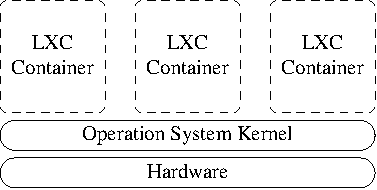
\includegraphics{graph/container01.pdf}
    \caption{容器架构模型}
  \label{fig:container}
\end{figure}

对于系统虚拟化技术来说,虚拟层为用户提供了一个完整的虚拟机:包括内核在
内的一个完整的系统镜像。CPU虚拟化技术可以为每个用户提供一个独享且和其他
用户隔离的系统环境,虚拟层可以为每个用户分配虚拟化后的CPU、内存和IO设备
资源,如图\ref{fig:virtualization}所示。

\begin{figure}[!htbp]
  \centering
  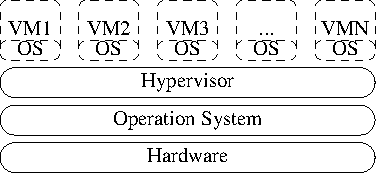
\includegraphics{graph/virtualization01.pdf}
    \caption{虚拟化架构模型}
  \label{fig:virtualization}
\end{figure}

\begin{verbatim}
git config --global user.name "Laven Liu"
git config --global user.email "air.man.six@gmail.com"
\end{verbatim}

\section{Docker简介}
\label{sec:introDocker}

\subsection{Docker与传统虚拟机建构对比}
\label{sec:contrastVM}

\subsection{应用容器虚拟化定位}
\label{sec:dockerDirect}

\subsection{Docker有哪些优势}
\label{sec:dockerAdvance}

\subsection{Docker应用场景}
\label{sec:dockerSec}

\subsection{Docker组成}
\label{sec:dockerComponents}

\section{安装及启动第一台Docker容器}
\label{sec:installDocker}

\section{测试环境}
\label{sec:dockerTestEnv}

Docker章节的演示在Ubuntu14.04 LTS 64位系统上进行演示\footnote{在此之前,
  作者是在CentOS6.5 64位系统上进行演示的,遇到过DeviceMapper的问题,甚
  至有时CentOS还会发生Kernel Panic的现象,故使用了Ubuntu系统进
  行Docker章节的演示。}。演示环境所使用的机器列表如下:

\begin{table}[htbp]
  \centering
    \caption{Docker演示环境机器一览}
    \label{tab:dockerMachines}
    \begin{tabular}{llr}
      \toprule
      主机名     & IP地址 & 说明 \\
      \midrule
      master01.lavenliu.com  & 192.168.20.134 &  主DNS \\
      minion01.lavenliu.com  & 192.168.20.135 &  辅DNS \\
      minion02.lavenliu.com  & 192.168.20.136 &  客户端 \\
      \bottomrule
    \end{tabular}
\end{table}

\subsection{安装Docker}
\label{installDocker}

在安装Docker之前,需要设置Docker官方的镜像源。

\begin{verbatim}
% sudo apt-get update
% sudo apt-get install docker-engine
% sudo status docker
\end{verbatim}

\begin{figure}[hbtp]
  \centering
  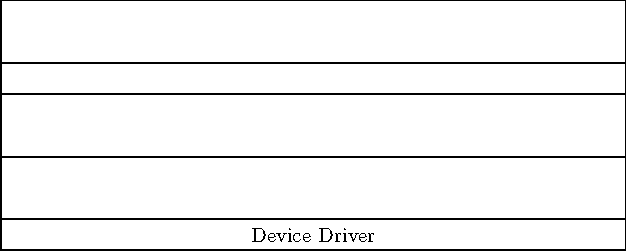
\includegraphics{graph/os-arch-mps.pdf}
    \caption{系统架构}
  \label{fig:OSArch}
\end{figure}

\subsection{运行第一台Docker容器}
\label{sec:runFirstDocker}

\section{容器及镜像管理}
\label{sec:containerManagement}

\subsection{容器管理}
\label{sec:containerManage}

\subsection{镜像管理}
\label{sec:dockerImageManage}

\section{构建Docker镜像}
\label{sec:buildDockerImage}

\subsection{手工构建}
\label{sec:buildDockerImgByHand}

\subsection{使用Dockerfile构建}
\label{sec:buildDockerImgByFile}


%%% Local Variables:
%%% mode: latex
%%% TeX-master: t
%%% End:


% OpenStack章节
\chapter{OpenStack}

\section{OpenStack简介}

\subsection{OpenStack常用组件介绍}
\label{sec:opAssemblyIntro}

\section{安装前的准备工作}
\label{sec:opPrepare}


%%% Local Variables:
%%% mode: latex
%%% TeX-master: t
%%% End:


% 公有云章节
\chapter{公有云}

\section{公有云简介}


%%% Local Variables:
%%% mode: latex
%%% TeX-master: t
%%% End:

\part{网络部分}
\label{part:network}

本部分主要介绍常用的网络协议及网络设备设备的基本使用。

\chapter{TCP/IP}
\label{chap:tcpIpProtocol}

\section{OSI网络参考模型}
\label{sec:osiModel}

\begin{figure}[!htbp]
  \centering
  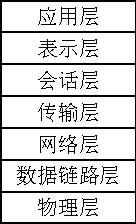
\includegraphics{graph/osi-1.pdf}
    \caption{OSI七层模型}
  \label{fig:osi}
\end{figure}

OSI参考模型有7层。适用于这7层的基本原则简要概括如下:\cite{computernetworks}
\begin{enumerate}[parsep=0pt]
\item 应该在需要一个不同抽象体的地方创建一层。
\item 每一层都应该执行一个明确定义的功能。
\item 每一层功能的选择应该向定义国际标准化协议的目标看齐。
\item 层与层边界的选择应该使跨越接口的信息流最小。
\item 层应该足够多,保证不同的功能不会被混杂在同一层,但同时层数不能太
  多,以免体系结构变得过于庞大。
\end{enumerate}

{\bfseries{物理层(physical layer):}}主要定义物理设备标准,如网线的接口
类型、光纤的接口类型、各种传输介质的传输率等。它的主要作用是传输比特
流\footnote{即由1、0转化为电流强弱来进行传输,到达目的地后再转化为1、0,
  也就是我们常说的数模转换与模数转换。}。这一层的数据叫做比特,网卡工作
在此层。一般物理层较少关心网络入侵分析,而更关注于保证设备的电缆安全。

{\bfseries{数据链路层(data link layer):}}主要将从物理层接收的数据进
行MAC地址(网卡的地址)的封装与解封装。这一层上的数据我们称为数据帧。在
这一层工作的设备是交换机,数据通过交换机来传输。

{\bfseries{网络层(network layer):}}主要将从下层收到的数据进行IP地址
的封装与解封装。在这一层工作的设备是路由器,我们称这一层的数据为数据包。

{\bfseries{传输层(transport layer):}}定义了一些传输数据的协议和端口
号,比如TCP\footnote{传输控制协议,传输效率低,可靠性强,用于传输可靠性
  要求高且数据量大的数据。}、UDP\footnote{用户数据报协议,与TCP的特性恰
  恰相反,用于传输可靠性要求不高且数据量小的数据。}。主要是将从下层接收
的数据进行分段,到达目的后进行数据重组。我们称这一层的数据为段。

{\bfseries{会话层(session layer):}}通过传输层(端口号:传输端口与接
收端口)建立数据传输的通路。主要在系统之间发起会话或接受会话请求(设备
之间可以通过IP,也可通过MAC或主机名来相互通信)。

{\bfseries{表示层(presentation layer):}}主要是接收的数据进行解释、加
密与解密、压缩与解压缩等(也就是把计算机能够识别的信息转化为人可以识别
的信息,如图片、声音等)。

{\bfseries{应用层(application layer):}}主要是一些终端应用,可把它理
解为应用层负责向用户或应用程序显示数据。

\subsection{TCP/IP三次握手}
\label{subsec:tcpIpThreeHandShake}

\subsection{TCP/IP四次挥手}
\label{subsec:tcpIpFourHandShake}

\chapter{H3C交换机配置}

\section{配置telnet方式登录}

\subsection{认证方式为Scheme时的登录配置}

\begin{verbatim}
sudo apt-get install git
sudo apt-get install git-core
\end{verbatim}

\section{以太网接口配置}

H3C交换机的配置如下:


配置方式与Cisco的很相似。

\begin{verbatim}
git config --global user.name "Laven Liu"
git config --global user.email "air.man.six@gmail.com"
\end{verbatim}

\subsection{打开或关闭以太网接口}
\label{sec:OpenShutInterface}

\begin{figure}[!htbp]
  \centering
  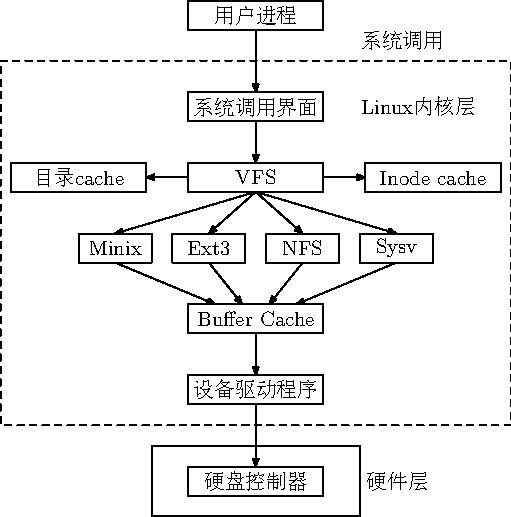
\includegraphics{graph/gnu-linux-0.pdf}
    \caption{Linux虚拟文件(测试图形)}
  \label{fig:LinuxVFS}
\end{figure}

\subsection{以太网端口基本属性配置}
\label{sec:BasicInterface}

\section{以太网接口的配置显示和维护}

\appendix
\part{附录部分}
\chapter{书中的源码}
\label{chap:sourceCode}

小白在写书过程中,书中用到了很多插图及少量的Bash脚本。这些插图都是小白
使用代码给绘制出来的。在此小白把自己所使用的工具及插图的源代码在本章里
给出。有需要的同志,可以随意修改,成为自己所需的图形。脚本的代码这里不
再给出。

为什么要使用这么古老的绘图工具?首先,小白使用的Ubuntu系统,上面没有安
装Office套件。这种图形看起来很专业\footnote{科技之类的文章好像都是这种
  形式};其次,绘制出的图形很精确\footnote{指哪画哪}。然而,它也有很大
缺点。首先,不可视化,很多人用不习惯(多用几次就好了)\footnote{编译之
  后才能看到效果};其次,不适合给领导做汇报用\footnote{使用PPT的方式或
  许更好,PPT越花哨越好}。

\section{第1章插图源码}

图\ref{fig:UnixTopo}的源代码,使用的绘图工具为metapost。如何编译生
成PDF图形呢?

\begin{verbatim}
# mpost -tex=latex source.mp
\end{verbatim}

\noindent 源码如下:
\begin{verbatim}
verbatimtex
\documentclass[10pt]{article}
\usepackage{CJK}
\AtBeginDocument{\begin{CJK}{UTF8}{gbsn}}
\AtEndDocument{\end{CJK}}
\begin{document}
etex
  
input boxes;
input rboxes;

% system variables
ahangle := 40;

% fig0 is linux virtual file system topo
beginfig(0);
  boxit.a(btex Shell解释程序 etex);
  boxit.b(btex \begin{tabular}{c}
      用户程序\quad各种应用程序包 \\
      系统命令\quad窗口命令\quad库函数
      \end{tabular} etex);
  boxit.c(btex 系统调用 etex);
  boxit.d(btex \begin{tabular}{c}
      核心层: \\
      存储管理\quad进程管理 \\
      设备管理\quad文件管理
      \end{tabular} etex);
  boxit.e(btex 硬件层 etex);
  a.sw = b.nw; a.se = b.ne;
  b.sw = c.nw; b.se = c.ne;
  c.sw = d.nw; c.se = d.ne;
  d.sw = e.nw; d.se = e.ne;
  a.se - a.sw = (140,0);
  b.se - b.sw = (140,0);
  c.se - c.sw = (140,0);
  d.se - d.sw = (140,0);
  e.se - e.sw = (140,0);

  circleit.cc(btex 用户 etex);
  circleit.dd(btex 用户 etex);

  cc.dx=cc.dy; dd.dx=dd.dy;

  cc.w = a.nw + (5,30);
  dd.e = a.ne - (5,-30);
  
  drawboxed(a,b,c,d,cc,dd);

  pair A[];
  A[1] = 1/3[a.nw,a.ne];
  A[2] = 2/3[a.nw,a.ne];
  draw cc.s -- A[1];
  draw dd.s -- A[2];

endfig;
end
\end{verbatim}

\section{第2章插图源码}

Libvirt拓扑图,

\begin{verbatim}
.PS
h = .1
dh = .02
dw = .1
[
	Userspacetools: [
		boxht = 2.5*h; boxwid = 8*dw; boxrad = dh
		movewid = 2*dh
		A: box "virsh"; move
		B: box "virt-manager"; move
		C: box "virt-viewer"; move
		D: box "virt-install"; move
		E: box "other tools"
	]
	Userspace: [
		boxht = 7*h; boxwid = 50*dw; boxrad = 2*dh
		AA: box
	] with .c at Userspacetools.c + (0,h/1.8)
	F: "Userspace Management Tools" at last [].n - (0,h+2*dh)

Libvirt: box ht 4*h wid 25*dw "Libvirt" "(Libvirt API)" with .n at last [].s - (0,3*h)

Hypervisoroutline: [
	Virtualtype: [
		boxht = 2*h; boxwid = 12*dw; boxrad = dh
		movewid = 2*dh
		A: box "VMware"; move
		B: box "Xen"; move
		C: box "KVM"; move
		D: box "Hyper-V"
	]
	Hypervisor: [
		boxht = 5*h; boxwid = 50*dw; boxrad = 2*dh
		AA: box
	] with .c at Virtualtype.c + (0,h/1.8)
	F: "Hypervisor Layer" at last [].n - (0,h+2*dh)
] with .n at Libvirt.s - (0,3*h)

XXX: [
	VMwareoutline: [
		VMware: [
			boxht = 3.5*h; boxwid = 5*dw; boxrad = dh
			movewid = 2*dh
			VM1: box "Guest 1"; move
			VM2: box "Guest 2"
		] with .n at Hypervisoroutline.Virtualtype.A.s - (0,3*h)
		box dashed ht last [].ht+dw wid last [].wid+dw at last []
	] 
	
	move 5*dh
	
	Xenoutline: [
		Xen: [
			 boxht = 3.5*h; boxwid = 5*dw; boxrad = dh
			 movewid = 2*dh
			 VM1: box "Dom0" "Guest"; move
			 VM2: box "DomU" "Guest"
		]
		box dashed ht last [].ht+dw wid last [].wid+dw at last []
	]

	move 5*dh

	Kvmoutline: [
		Kvm: [
			 boxht = 1.75*h; boxwid = 5*dw; boxrad = dh
			 movewid = 2*dh
			 VM1: [
			 	  Qemu1: box "Qemu"
			 	  Guest01: box "Guest 1" with .n at Qemu1.s
			 ]
			 
			 move
			 
			 VM2: [
			 	  Qemu1: box "Qemu"
				  Guest01: box "Guest 2" with .n at Qemu1.s
			 ]
		]
		box dashed ht last [].ht+dw wid last [].wid+dw at last []
	]
	
	move 5*dh

	Hypervoutline: [
		Hyperv: [
			boxht = 3.5*h; boxwid = 5*dw; boxrad = dh
			movewid = 2*dh
			VM1: box "Guest 1"; move
			VM2: box "Guest 2"
		]
		box dashed ht last [].ht+dw wid last [].wid+dw at last []
	]
] with .n at last [].s - (0,3*h)

arrow from Userspacetools.A.s to Libvirt.nw
arrow from Userspacetools.B.s to 1/2 <Libvirt.nw,Libvirt.n>
arrow from Userspacetools.C.s to Libvirt.n
arrow from Userspacetools.D.s to 1/2 <Libvirt.n,Libvirt.ne>
arrow from Userspacetools.E.s to Libvirt.ne

arrow from Libvirt.s to 3rd [].Hypervisor.n

arrow from Hypervisoroutline.Virtualtype.A.s to XXX.VMwareoutline.VMware.n
arrow from Hypervisoroutline.Virtualtype.B.s to XXX.Xenoutline.Xen.n
arrow from Hypervisoroutline.Virtualtype.C.s to XXX.Kvmoutline.Kvm.n
arrow from Hypervisoroutline.Virtualtype.D.s to XXX.Hypervoutline.Hyperv.n

]
.PE
\end{verbatim}

libvirt与node与hypervisor,

\begin{verbatim}
.PS
[
		A: [
		   box dashed wid 0.7 ht 0.75 rad 0.05 "Domain 1"
		   move 0.2
		   box dashed wid 0.7 ht 0.75 rad 0.05 "Domain 2"
		   move same
		   box dashed wid 0.7 ht 0.75 rad 0.05 "Domain N"
		]

		B: [
		   box wid 2.5 ht 0.2 rad 0.1 "Hypervisor"
  		] with .n at A .s - (0,0.15)
]

box ht last [].ht+0.45 wid last [].wid+0.3 at last [] + (0,0.05)
"Node" at last box .n - (0,0.15)
.PE
\end{verbatim}

KVM桥接网络,

\begin{verbatim}
.PS
[
		A: [
		   box dashed wid 0.7 ht 0.75 rad 0.05 "Domain 1"
		   move 0.2
		   box dashed wid 0.7 ht 0.75 rad 0.05 "Domain 2"
		   move same
		   box dashed wid 0.7 ht 0.75 rad 0.05 "Domain N"
		]

		B: [
		   box wid 2.5 ht 0.2 rad 0.1 "Hypervisor"
  		] with .n at A .s - (0,0.15)
]

box ht last [].ht+0.45 wid last [].wid+0.3 at last [] + (0,0.05)
"Node" at last box .n - (0,0.15)
.PE
\end{verbatim}

saltstack通讯模型,

\begin{verbatim}
.PS
scale = 2.54

define port { [
       Port: box wid $1 ht $2 $3 "$4"
       ]
}

Master: box wid 5.5 ht 2 rad 0.2;

"master" at Master.n below;

Port4505: [ port(2,1,"Publish Port",4505) ] with .se at Master.s - (0.25,0);
Port4506: [ port(2,1,"Return Port",4506) ] with .sw at Master.s + (0.25,0);

Minion1: [ box wid 1.5 ht 1 rad 0.1 "minion1" ] with .nw at Master.sw - (0,1.5);
Minion2: [ box wid 1.5 ht 1 rad 0.1 "minion2" ] with .ne at Master.se - (0,1.5);

line -> from 1/3 <Port4505.sw,Port4505.se> to 1/3 <Minion1.nw,Minion1.ne>;
line -> from 1/3 <Port4505.se,Port4505.sw> to 1/3 <Minion2.nw,Minion2.ne>;
line -> from 2/3 <Minion1.nw,Minion1.ne> to 1/3 <Port4506.sw,Port4506.se> dashed;
line -> from 2/3 <Minion2.nw,Minion2.ne> to 2/3 <Port4506.sw,Port4506.se> dashed;
.PE
\end{verbatim}

ELK拓扑图,

\begin{verbatim}
.PS

define shipper {
	box wid $1 ht $2 rad $3 "Shipper" "LogStash";
}

[
	shipper(0.85,0.4,0.02);
]

[
	shipper(0.85,0.4,0.02);
] with .n at last [].s - (0,0.35);

[
	shipper(0.85,0.4,0.02);
] with .n at last [].s - (0,0.35);

Broker: circle rad 0.5 "Borker" "Redis" "192.168.20.138" with .w at 2nd [].e + (0.35,0);

move right 0.35;

Indexer: box wid 1.15 ht 0.55 rad 0.02 "Indexer" "LogStash" "192.168.20.139";

move same;

Elastic: box wid 1.15 ht 0.75 rad 0.02 "Search &" "Storage" "ElasticSearch" "192.168.20.139";

move same;

Kibana: box wid 1.15 ht 1.9 rad 0.02 "Web" "Interface" "LogStash" "192.168.20.139";

point01 = 1st [].e.y;
Line1: line right from 1st [].e to (Broker.n.x,point01);
line -> from Line1.end to Broker.n;

point02 = last [].e.y;
Line2: line right from last [].e to (Broker.s.x,point02);
line -> from Line2.end to Broker.s;

line -> from 2nd [] .e to Broker.w;
line -> from Broker.e to Indexer.w;
line -> from Indexer.e to Elastic.w;
line -> from Kibana.w to Elastic.e;
.PE
\end{verbatim}

AWK工作流程图,

\begin{verbatim}
.PS
A: box ht 0.8 rad 0.08 "Line 1" "Line 2" "Line 3" "Line 4" "..."
INFILE: "\fBInput file\fP" with .n at A.s - (0,0.15)
B: box width 1.8 "Read a Line" with .nw at A.ne + (0.5,0)
C: box width 1.8 "Execute awk commands" "in the \fBbody\fP block on the line" at B - (0,0.8)
D: box width 1.8 "\fBRepeat\fP for the next line until" "end of the input file" at C - (0,0.8)
E: box width 1.8 rad 0.1 "Execute awk commands in" "the \fBEND\fP Block" at D - (0,0.8)
F: box width 1.8 "Execute awk commands in" "the \fBBEGIN\fP Block" at B + (0,0.8)

L1: line chop 0.01 chop 0.9 from 1st box at 1/3 <A.e,A.ne> to B ->

L2: line down from B to C -> chop
L3: arrow down from C to D chop
L4: arrow down from D to E chop

L5: line down 2 from L1 .center
L6: line right from L5.end to L4.center
L7: arrow  from F.s to B.n
.PE
\end{verbatim}

SED工作流程图,

\begin{verbatim}
.PS
A: box ht 0.8 rad 0.08 "Line 1" "Line 2" "Line 3" "Line 4" "..."
INFILE: "\fBInput file\fP" with .n at A.s - (0,0.15)
B: box width 1.8 "\fBRead\fP a line into the" "pattern space" with .nw at A.ne + (0.5,0)
C: box width 1.8 "\fBExecute\fP given sed commands" "on the pattern space" at B - (0,0.8)
D: box width 1.8 "\fBPrint\fP the pattern space" "and empty it" at C - (0,0.8)
E: box width 1.8 "\fBRepeat\fP for the next line until" "end of the input file" at D - (0,0.8)
F: box width 0.75 ht 0.35 rad 0.05 "Line 1" with .w at B.e + (0.35,0)
PATTERN: "\fBPattern space\fP" with .n at F.s - (0,0.15)
G: circle "Output" with .w at D.e + (0.35,0)

L1: line chop 0.01 chop 0.9 from 1st box at 1/3 <A.e,A.ne> to B ->

L2: line down from B to C -> chop
L3: arrow down from C to D chop
L4: arrow down from D to E chop

L5: line dashed from B.e to F.w ->
L6: line dashed from C.e to F.w ->
L7: line dashed from D.e to G.w ->

L8: line down 2.85 from L1 .center to E.sw - (0.2,0.2)
L9: line right from L8.end to E.s - (0,0.2)
L10: line from E.s to L9.end
.PE
\end{verbatim}

Linux模型,

\begin{verbatim}
verbatimtex
\documentclass[10pt]{article}
\usepackage{CJK}
\AtBeginDocument{\begin{CJK}{UTF8}{gbsn}}
\AtEndDocument{\end{CJK}}
\begin{document}
etex
  
input boxes;
input rboxes;

% system variables
ahangle := 40;

% fig0 is linux virtual file system topo
outputtemplate := "vfs.mps";
beginfig(0);
  defaultfont:="ptmr8r";
  boxit.a(btex 用户进程 etex);
  boxit.b(btex 系统调用界面 etex);
  boxit.c(btex VFS etex);
  boxit.d(btex Ext3 etex);
  boxit.e(btex Buffer Cache etex);
  boxit.f(btex 设备驱动程序 etex);
  boxit.g(btex 硬盘控制器 etex);
  boxit.minix(btex Minix etex);
  boxit.nfs(btex NFS etex);
  boxit.sysv(btex Sysv etex);
  boxit.direc(btex 目录cache etex);
  boxit.inode(btex Inode cache etex);
  boxit.hard(btex etex);

  % Len is the box's length
  % Hig is the box's hight
  numeric Len;
  numeric Hig;
  Len := 65;
  Hig := 14pt;
  a.e - a.w = (Len,0); a.n - a.s = (0,Hig);
  b.e - b.w = (Len,0); b.n - b.s = (0,Hig);
  c.e - c.w = (Len,0); c.n - c.s = (0,Hig);
  d.e - d.w = (35,0); d.n - d.s = (0,Hig);
  minix.e - minix.w = (35,0); minix.n - minix.s = (0,Hig);
  nfs.e - nfs.w = (35,0); nfs.n - nfs.s = (0,Hig);
  sysv.e - sysv.w = (35,0); sysv.n - sysv.s = (0,Hig);
  e.e - e.w = (Len,0); e.n - e.s = (0,Hig);
  f.e - f.w = (Len,0); f.n - f.s = (0,Hig);
  g.e - g.w = (Len,0); g.n - g.s = (0,Hig);
  direc.e - direc.w = (Len,0); direc.n - direc.s = (0,Hig);
  inode.e - inode.w = (Len,0); inode.n - inode.s = (0,Hig);

  % Dis is the hight between the boxes
  numeric Dis;
  Dis := 20;
  a.s - b.n = (0,30);
  b.s - c.n = (0,Dis);
  c.s - d.ne = (5,Dis);
  d.se - e.n = (-5,Dis);
  c.s - nfs.nw = (-5,Dis);
  d.w - minix.e = (10,0);
  sysv.w - nfs.e = (10,0);
  e.s - f.n = (0,Dis);
  f.s - g.n = (0,30);
  c.w - direc.e = (Dis,0);
  c.e - inode.w = (-Dis,0);
  hard.c = g.c;
  hard.e - hard.w = (100,0);
  hard.n - hard.s = (0,34);
  drawboxed(a,b,c,d,e,f,g,minix,nfs,sysv,direc,inode,hard);

  % draw the connectors
  drawarrow a.s -- b.n;
  drawarrow b.s -- c.n;
  
  drawarrow c.s -- minix.n;
  drawarrow c.s -- d.n;
  drawarrow c.s -- nfs.n;
  drawarrow c.s -- sysv.n;

  pair A[];
  A[1] = 1/5[e.nw,e.ne];
  A[2] = 2/5[e.nw,e.ne];
  A[3] = 3/5[e.nw,e.ne];
  A[4] = 4/5[e.nw,e.ne];
  drawarrow minix.s -- A[1];
  drawarrow d.s -- A[2];
  drawarrow nfs.s -- A[3];
  drawarrow sysv.s -- A[4];

  drawarrow e.s -- f.n;
  drawarrow f.s -- g.n;

  drawarrow c.w -- direc.e;
  drawarrow c.e -- inode.w;

  % draw the outline
  pair B[];
  B[1] = direc.w - (5,-56);
  B[2] = inode.e - (-5,-56);
  B[3] = inode.e - (-5,119);
  B[4] = direc.w - (5,119);

  draw B[1] -- B[2] -- B[3] -- B[4] -- cycle dashed evenly;
  label.rt(btex 硬件层 etex,hard.e);
  label.rt(btex Linux内核层 etex,b.e+(15,0));
  label.rt(btex 系统调用 etex,a.se+(15,-5));
endfig;

outputtemplate := "os-arch.mps";
beginfig(1);
  boxjoin(a.nw=b.sw; a.ne=b.se);
  boxit.a(btex Device Driver etex);
  boxit.b();
  boxit.c();
  boxit.d();
  boxit.e();

  numeric Len[],Hig[];
  Len[1] := 300;
  Hig[1] := 15;
  Hig[2] := 30;
  a.e - a.w = (Len[1],0); a.n - a.s = (0,Hig[1]);
  b.n - b.s = (0,Hig[2]); c.n - c.s = (0,Hig[2]);
  d.n - d.s = (0,Hig[1]); e.n - e.s = (0,Hig[2]);
  drawboxed(a,b,c,d,e);

endfig;

outputtemplate := "osarch.mps";
beginfig(2);
  boxjoin(a.nw=b.sw; a.ne=b.se);
  boxit.a(btex Block Device Driver etex);
  boxit.b(btex Volume Manager etex);
  boxit.c(btex File Systems etex);
  boxit.d(btex VFS etex);

  boxjoin(e.nw=f.sw; e.ne=f.se);
  boxit.e(btex Ethernet etex);
  boxit.f(btex IP etex);
  boxit.g(btex TCP/UDP etex);
  boxit.h(btex Socket etex);

  e.nw = a.ne; e.sw = a.se;  
  numeric Len[],Hig[];
  Len[1] := 95;
  Hig[1] := 15;
  Hig[2] := 30;
  a.e - a.w = (Len[1],0); a.n - a.s = (0,Hig[1]);
  b.n - b.s = (0,Hig[1]); c.n - c.s = (0,Hig[1]);
  d.n - d.s = (0,Hig[1]); e.n - e.s = (0,Hig[1]);
  f.n - f.s = (0,Hig[1]); g.n - g.s = (0,Hig[1]);

  drawboxed(a,b,c,d,e,f,g,h);
endfig;
end
\end{verbatim}

\section{第14章插图源码}
\label{sec:index14}

图\ref{fig:container}的源码,使用的是pic工具进行绘制的。源码为:

\begin{verbatim}
.PS
define container { [
    box dashed wid 0.7 ht 0.75 rad 0.05 "$1" "Container"
] }

define layer {
    box wid 2.5 ht 0.2 rad 0.1 "$1"
}

V1: container(LXC)
move 0.2
V2: container(LXC)
move same
V3: container(LXC)

move to V1.sw - 0,0.15

L1: layer(Operation System Kernel)
move to L1.s - 0,0.05
down
L2: layer(Hardware)
.PE
\end{verbatim}

图\ref{fig:virtualization}的源码,使用的pic工具进行绘制的。源码为:

\begin{verbatim}
.PS
define vm { [
    box dashed wid 0.4 ht 0.4 rad 0.05 "$1"
    box dashed wid 0.4 ht 0.13 rad 0.05 "OS" with .s at last box .s
] }

define layer {
    box wid 2.5 ht 0.2 rad 0.1 "$1"
}

V1: vm(VM1)
move 0.125
V2: vm(VM2)
move same
V3: vm(VM3)
move same
V4: vm(...)
move same
V5: vm(VMN)

move to V1.sw - 0,0.15

L1: layer(Hypervisor)
move to L1.s - 0,0.05
down
L2: layer(Operation System)
move to L2.s - 0,0.05
down
L3: layer(Hardware)
.PE
\end{verbatim}

如何编译呢?

\begin{verbatim}
pic /path/to/filename.pic | groff | ps2eps > /path/to/filename.eps
epstopdf /path/to/filename.eps
evince /path/to/filename.pdf
# 如果是Windows系统,则可以使用Adobe Reader或福昕阅读器进行查看
\end{verbatim}

\bibliography{body/mybib}

\printindex
\clearpage
\end{document}

%%% Local Variables:
%%% mode: latex
%%% TeX-master: t
%%% End:
